\documentclass[oneside]{book}
\usepackage[backend=biber,natbib=true,style=alphabetic,maxbibnames=50]{biblatex}
\addbibresource{/home/nqbh/reference/bib.bib}
\usepackage[utf8]{vietnam}
\usepackage{tocloft}
\renewcommand{\cftsecleader}{\cftdotfill{\cftdotsep}}
\usepackage[colorlinks=true,linkcolor=blue,urlcolor=red,citecolor=magenta]{hyperref}
\usepackage{amsmath,amssymb,amsthm,enumitem,fancyvrb,float,graphicx,mathtools,minitoc,tikz}
\usetikzlibrary{angles,calc,intersections,matrix,patterns,quotes,shadings}
\usepackage{fancyhdr}
\pagestyle{fancy}
\fancyhf{}
\addtolength{\headheight}{0pt}% obsolete
\lhead{\scshape\small\chaptername~\thechapter}
\rhead{\small\nouppercase{\leftmark}}
\renewcommand{\chaptermark}[1]{\markboth{#1}{}}
\cfoot{\thepage}
\renewcommand{\headrulewidth}{0.5pt}
\renewcommand{\footrulewidth}{0pt}
\fancyheadoffset[RE,LO]{-0.0\textwidth}

\usepackage{textcase}

\makeatletter
\def\@makechapterhead#1{%
    \vspace*{50\p@}%
    {\parindent \z@ \centering\normalfont
        \ifnum \c@secnumdepth >\m@ne
        \if@mainmatter
        \huge\bfseries \MakeTextUppercase{\@chapapp}\space \thechapter
        \par\nobreak
        \vskip 20\p@
        \fi
        \fi
        \interlinepenalty\@M
        \huge \bfseries \MakeTextUppercase{#1}\par\nobreak
        \vskip 40\p@
}}
\def\@makeschapterhead#1{%
    \vspace*{50\p@}%
    {\parindent \z@ \centering
        \normalfont
        \interlinepenalty\@M
        \huge \bfseries  \MakeTextUppercase{#1}\par\nobreak
        \vskip 40\p@
}}
\makeatother


\DeclareMathSymbol{\mathinvertedexclamationmark}{\mathclose}{operators}{'074}
\DeclareMathSymbol{\mathexclamationmark}{\mathclose}{operators}{'041}

\makeatletter
\newcommand{\raisedmathinvertedexclamationmark}{%
    \mathclose{\mathpalette\raised@mathinvertedexclamationmark\relax}%
}
\newcommand{\raised@mathinvertedexclamationmark}[2]{%
    \raisebox{\depth}{$\m@th#1\mathinvertedexclamationmark$}%
}
\begingroup\lccode`~=`! \lowercase{\endgroup
    \def~}{\@ifnextchar`{\raisedmathinvertedexclamationmark\@gobble}{\mathexclamationmark}}
\mathcode`!="8000
\makeatother

\usepackage{sectsty}
\allsectionsfont{\sffamily}
\allowdisplaybreaks
\newtheorem{assumption}{Assumption}
\newtheorem{baitoan}{Bài toán}
\newtheorem{cauhoi}{Câu hỏi}
\newtheorem{conjecture}{Conjecture}
\newtheorem{corollary}{Corollary}
\newtheorem{dangtoan}{Dạng toán}
\newtheorem{definition}{Definition}
\newtheorem{dinhly}{Định lý}
\newtheorem{dinhnghia}{Định nghĩa}
\newtheorem{example}{Example}
\newtheorem{ghichu}{Ghi chú}
\newtheorem{goal}{Goal}
\newtheorem{hequa}{Hệ quả}
\newtheorem{hypothesis}{Hypothesis}
\newtheorem{intuition}{Intuition}
\newtheorem{lemma}{Lemma}
\newtheorem{luuy}{Lưu ý}
\newtheorem{nhanxet}{Nhận xét}
\newtheorem{notation}{Notation}
\newtheorem{note}{Note}
\newtheorem{principle}{Principle}
\newtheorem{problem}{Problem}
\newtheorem{proposition}{Proposition}
\newtheorem{question}{Question}
\newtheorem{remark}{Remark}
\newtheorem{theorem}{Theorem}
\newtheorem{vidu}{Ví dụ}
\usepackage[left=1cm,right=1cm,top=1.5cm,bottom=1.5cm]{geometry}
\def\labelitemii{$\circ$}
\DeclareRobustCommand{\divby}{%
    \mathrel{\vbox{\baselineskip.65ex\lineskiplimit0pt\hbox{.}\hbox{.}\hbox{.}}}%
}
\setlist[itemize]{leftmargin=*}
\setlist[enumerate]{leftmargin=*}
\newcommand{\genstirlingI}[3]{%
    \genfrac{[}{]}{0pt}{#1}{#2}{#3}%
}
\newcommand{\genstirlingII}[3]{%
    \genfrac{\{}{\}}{0pt}{#1}{#2}{#3}%
}
\newcommand{\stirlingI}[2]{\genstirlingI{}{#1}{#2}}
\newcommand{\dstirlingI}[2]{\genstirlingI{0}{#1}{#2}}
\newcommand{\tstirlingI}[2]{\genstirlingI{1}{#1}{#2}}
\newcommand{\stirlingII}[2]{\genstirlingII{}{#1}{#2}}
\newcommand{\dstirlingII}[2]{\genstirlingII{0}{#1}{#2}}
\newcommand{\tstirlingII}[2]{\genstirlingII{1}{#1}{#2}}

\title{Olympiad in Informatics {\it\&} Association for Computing Machinery--International Collegiate Programming Contest\\Olympic Tin Học Sinh Viên OLP {\it\&} ACM-ICPC}
\author{Nguyễn Quản Bá Hồng\footnote{A scientist- {\it\&} creative artist wannabe, a mathematics {\it\&} computer science lecturer of Department of Artificial Intelligence {\it\&} Data Science (AIDS), School of Technology (SOT), UMT Trường Đại học Quản lý {\it\&} Công nghệ TP.HCM, Hồ Chí Minh City, Việt Nam.\\E-mail: {\sf nguyenquanbahong@gmail.com} {\it\&} {\sf hong.nguyenquanba@umt.edu.vn}. Website: \url{https://nqbh.github.io/}. GitHub: \url{https://github.com/NQBH}.}}
\date{\today}

\begin{document}
\maketitle
\setcounter{secnumdepth}{4}
\setcounter{tocdepth}{4}
\dominitoc % Initialization
\tableofcontents

%------------------------------------------------------------------------------%

\chapter*{Preface}
\minitoc

%------------------------------------------------------------------------------%
\section*{Abstract}
This text is a part of the series {\it Some Topics in Advanced STEM \& Beyond}:

{\sc url}: \url{https://nqbh.github.io/advanced_STEM/}.

Latest version:
\begin{itemize}
    \item {\it Olympiad in Informatics \& Association for Computing Machinery--International Collegiate Programming Contest -- Olympic Tin Học Sinh Viên OLP \& ICPC}.
    
    PDF: {\sc url}: \url{https://github.com/NQBH/advanced_STEM_beyond/blob/main/OLP_ICPC/NQBH_OLP_ICPC.pdf}.
    
    \TeX: {\sc url}: \url{https://github.com/NQBH/advanced_STEM_beyond/blob/main/OLP_ICPC/NQBH_OLP_ICPC.tex}.
    \item Codes:
    \begin{itemize}
        \item C: \url{https://github.com/NQBH/advanced_STEM_beyond/tree/main/OLP_ICPC/C}.
        \item C++: \url{https://github.com/NQBH/advanced_STEM_beyond/tree/main/OLP_ICPC/C++}.
        \item Python: \url{https://github.com/NQBH/advanced_STEM_beyond/tree/main/OLP_ICPC/Python}.
    \end{itemize}
\end{itemize}

%------------------------------------------------------------------------------%

\chapter*{Preliminaries -- Kiến thức chuẩn bị}
\minitoc

%------------------------------------------------------------------------------%

\textbf{\textsf{Resources -- Tài nguyên.}}
\begin{enumerate}
	\item \cite{Wu_Wang2016}. {\sc Yonghui Wu, Jiande Wang}. {\it Data Structure Practice for Collegiate Programming Contests \& Education}.
	\item \cite{Wu_Wang2018}. {\sc Yonghui Wu, Jiande Wang}. {\it Algorithm Design Practice for Collegiate Programming Contests \& Education}.	
	\item Codeforces \url{https://codeforces.com/}.
	\item CSES Problem Sets. \url{https://cses.fi/problemset/}.
\end{enumerate}
Some critical-thinking questions:
\begin{question}[Generalization; main ideas of a solution{\tt/}proof]
	What are main ideas of a solution or a proof of a problem that can be used to generalize the original problem?
\end{question}

\begin{question}[Link\footnote{Watch, e.g., \href{https://www.imdb.com/title/tt14976292/}{IMDb{\tt/}Shi Guang Dai Li Ren $\star$ Link Click} (2021--).}]
	Can we draw some link(s) between different problems? Even they are in different categories: algebra, analysis, \& combinatorics.
\end{question}

\begin{remark}[Repeat \& mathematical induction -- Lặp \& quy nạp toán học]
	\label{rmk: repeat}
	Nếu bài toán có chứa $n\in\mathbb{N}^\star$ tổng quát hoặc chứa số tự nhiên của năm ra đề, e.g., 2025, thì đưa $2025$ về $n\in\mathbb{N}^\star$, rồi sử dụng các kỹ thuật toán học để đưa về phép lặp, hoặc sử dụng phương pháp quy nạp toán học (method mathematical induction).
\end{remark}

\section*{Notation -- Ký hiệu}

\begin{itemize}
	\item $\overline{m,n}\coloneqq\{m,m + 1,\ldots,n - 1, n\}$, $\forall m,n\in\mathbb{Z}$, $m\le n$. Hence the notation ``for $i\in\overline{m,n}$'' means ``for $i = m,m + 1,\ldots,n$'', i.e., chỉ số{\tt/}biến chạy $i$ chạy từ $m\in\mathbb{Z}$ đến $n\in\mathbb{Z}$. Trong trường hợp $a,b\in\mathbb{R}$, ký hiệu $\overline{a,b}\coloneqq\overline{\lceil a\rceil,\lfloor b\rfloor}$ có nghĩa như định nghĩa trước đó với $m\coloneqq\lceil a\rceil,n\coloneqq\lfloor b\rfloor\in\mathbb{Z}$; khi đó ký hiệu ``for $i\in\overline{a,b}$'' với $a,b\in\mathbb{R}$, $a\le b$ có nghĩa là ``for $i = \lceil a\rceil,\lceil a\rceil + 1,\ldots,\lfloor b\rfloor - 1,\lfloor b\rfloor$, i.e., chỉ số{\tt/}biến chạy $i$ chạy từ $\lceil a\rceil$ đến $\lfloor b\rfloor\in\mathbb{Z}$.
	\item $\lfloor x\rfloor,\{x\}$ lần lượt được gọi là {\it phần nguyên \& phần lẻ} (integer- \& fractional parts) của $x\in\mathbb{R}$, see, e.g., \href{https://en.wikipedia.org/wiki/Floor_and_ceiling_functions}{Wikipedia{\tt/}floor \& ceiling functions}, \href{https://en.wikipedia.org/wiki/Fractional_part}{Wikipedia{\tt/}fractional part}.
	\item $x_+\coloneqq\max\{x,0\}$, $x_-\coloneqq\max\{-x,0\} = -\min\{x,0\}$ lần lượt được gọi là {\it phần dương \& phần âm} (positive- \& negative parts) của $x\in\mathbb{R}$.
	\item s.t.: abbreviation of `such that'.
	\item w.l.o.g.: abbreviation of `without loss of generality'.
\end{itemize}

\begin{question}[MO $\mapsto$ OI: Mathematical Olympiads $\mapsto$ Olympiads of Informatics]
    Những bài Olympic Toán học, e.g., VMO, USAMO, China MO, đặc biệt là IMO, IMO shortlists, etc. nào có thể code được? Đưa các tiêu chí cho việc code-able.
\end{question}

\begin{proof}[Answer]
    Trước hết các bài toán Olympic có thể code được gồm các bài về mảng số (arrays of real numbers, or finite sequence of real numbers), dãy số (infinite sequences of of real numbers), hình học tính toán (computational geometry), hình học tổ hợp (combinatorial geometry), số học{\tt/}lý thuyết số (number theory). Đối với từng bài, mới biết có thể ra bài Olympic Tin tương ứng hay không, \& còn tùy thuộc vào trình độ của người chế đề.
    
    Các bài hình học thiên về thuần chứng minh thường khó ra đề Olympic Tin tương ứng 1 cách trực tiếp được, trừ khi là {\tt AlphaGeometry}. Prove me wrong.
\end{proof}

%------------------------------------------------------------------------------%

\part{Introduction to Programming -- Nhập Môn Lập Trình}
\minitoc

%------------------------------------------------------------------------------%

\part{Programming Techniques -- Kỹ Thuật Lập Trình}
\minitoc

%------------------------------------------------------------------------------%

\chapter{Pointer Variable \& Dynamic Memory Technique -- Biến Con Trỏ \& Kỹ Thuật Bộ Nhớ Động}
\minitoc

%------------------------------------------------------------------------------%

\chapter{Linked Lists -- Danh Sách Liên Kết}
\minitoc

%------------------------------------------------------------------------------%

\chapter{Abstract Data Structure Installation -- Cài Đặt Cấu Trúc Dữ Liệu Trừu Tượng}
\minitoc

%------------------------------------------------------------------------------%

\chapter{Strings \& Algorithms -- Chuỗi Ký Tự \& Thuật Toán}
\minitoc

%------------------------------------------------------------------------------%

\chapter{Search Algorithms \& Applications -- Thuật Toán Tìm Kiếm \& Ứng Dụng}
\minitoc

%------------------------------------------------------------------------------%

\chapter{Sort Algorithms \& Applications -- Thuật Toán Sắp Xếp \& Ứng Dụng}
\minitoc

%------------------------------------------------------------------------------%

\chapter{Recursion Programming -- Lập Trình Đệ Quy}
\minitoc

%------------------------------------------------------------------------------%

\chapter{Dynamic Programming Techniques -- Kỹ Thuật Quy Hoạch Động}
\minitoc

%------------------------------------------------------------------------------%

\chapter{Functional Pointers \& Variable Sourcecodes -- Con Trỏ Hàm \& Mã Nguồn Tùy Biến}
\minitoc

%------------------------------------------------------------------------------%

\part{Competitive Programming -- Lập Trình Thi Đấu}
\minitoc

%------------------------------------------------------------------------------%

\chapter{Basic Competitive Programming -- Lập Trình Thi Đấu Cơ Bản}
\minitoc

%------------------------------------------------------------------------------%

\textbf{\textsf{Resources -- Tài nguyên.}}
\begin{enumerate}
	\item \cite{Laaksonen2020}. {\sc Antti Laaksonen}. {\it Guide to Competitive Programming: Learning \& Improving Algorithms Through Contests}.
    
	\item \cite{Thu_Phuong_Tien_Triet_NMLT}. {\sc Trần Đan Thư, Nguyễn Thanh Phương, Đinh Bá Tiến, Trần Minh Triết}. {\it Nhập Môn Lập Trình}.
    
	\item \cite{Thu_Phuong_Tien_Triet_Phuong_KTLT}. {\sc Trần Đan Thư, Nguyễn Thanh Phương, Đinh Bá Tiến, Trần Minh Triết, Đặng Bình Phương}. {\it Kỹ Thuật Lập Trình}.
    
	\item \cite{Thu_Tien_Khang_PPLTHDT}. {\sc Trần Đan Thư, Đinh Bá Tiến, Nguyễn Tấn Trần Minh Khang}. {\it Phương Pháp Lập Trình Hướng Đối Tượng}.
\end{enumerate}

\section{The art of handling inputs \& formatting outputs -- Nghệ thuật xử lý các dạng đầu vào \& định dạng các dạng đầu ra}
To handle various types of inputs \& format various types of outputs, see, e.g.:
\begin{itemize}
	\item \href{http://poj.org/faq.htm}{Peking University Judge Online for ACM{\tt/}ICPC (POJ){\tt/}FAQ}.
	See, e.g., \cite[Chap. 2, Subsect. 2.1.1, pp. 10--11]{Laaksonen2020, Laaksonen2024}.
\end{itemize}
To compile a C++ program in Linux, run in Terminal:
\begin{verbatim}
$ g++ -O2 -Wall program_name.cpp -o program_name
$ ./program_name
\end{verbatim}
or if you want to transfer input file into it \& print output into Terminal screen:
\begin{verbatim}
$ ./program_name < program_name.inp
\end{verbatim}
or if you want to transfer input file into it \& print output into a file:
\begin{verbatim}
$ ./program_name < program_name.inp > program_name.out
\end{verbatim}

\begin{itemize}
	\item Geeks4Geeks{\tt/std::endl} vs. \verb|\n| in C++: \url{https://www.geeksforgeeks.org/endl-vs-n-in-cpp/}. 
	\item {\tt i++} vs. {\tt++i}: \href{https://stackoverflow.com/questions/24886/is-there-a-performance-difference-between-i-and-i-in-c}{StackOverflow{\tt/}Is there a performance difference between i++ \& ++i in C?}
\end{itemize}

\section{Repeat{\tt/}Loop -- Lặp}

\section{String data -- Kiểu dữ liệu chuỗi}

%------------------------------------------------------------------------------%

\section{Array data -- Kiểu dữ liệu mảng}
Về mặt toán học, kiểu dữ liệu mảng là dãy số hữu hạn $(a_i)_{i=1}^n = (a_1,a_2,\ldots,a_n)$. Về mặt Tin học, kiểu dữ liệu mảng được ký hiệu bởi {\tt a[1..n]}.

\begin{baitoan}[\cite{Duc_200_BT_Python}, 141., pp. 140--141: Count digit -- Đếm chữ số]
	Cho dãy số $n$ số nguyên dương $A[1..n]$ \& 1 chữ số $k$. Đếm số lần xuất hiện chữ số $k$ trong dãy $A$ đã cho. E.g., với dãy $A[] = (11,12,13,14,15)$, thì chữ số $k = 1$ xuất hiện $6$ lần trong dãy $A$.
	\item {\sf Input.} Dòng 1 của đầu vào chứa số nguyên $T\in\mathbb{N}^\star$ cho biết số bộ dữ liệu cần kiểm tra. Mỗi bộ dữ liệu gồm: (i) Dòng đầu chứa lần lượt $n,k\in\mathbb{N}$ là số phần tử trong dãy $A[]$ \& chữ số $k$. (ii) Dòng 2 chứa $n$ số nguyên cách nhau 1 dấu cách, mô tả các phần tử của dãy $A$.
	\item {\sf Output.} Ứng với mỗi bộ dữ liệu, in ra 1 dòng chứa kết quả của bài toán tương ứng với bộ dữ liệu đầu vào đó.
	\item {\sf Constraint.} $1\le T\le100,1\le n\le100,0\le k\le9,1\le A[i]\le1000$, $\forall i = 1,\ldots,n$.
\end{baitoan}

\begin{itemize}
	\item Input: \url{https://github.com/NQBH/advanced_STEM_beyond/blob/main/OLP_ICPC/input/count_digit.inp}.
	\item Output: \url{https://github.com/NQBH/advanced_STEM_beyond/blob/main/OLP_ICPC/output/count_digit.out}.
	\item Python: \url{https://github.com/NQBH/advanced_STEM_beyond/blob/main/OLP_ICPC/Python/count_digit.py}.
	\item C++: ?
\end{itemize}

\begin{baitoan}[\cite{Duc_200_BT_Python}, 141., pp. 140--141: Count digit -- Đếm chữ số]
	Cho dãy số nguyên $a[1],a[2],\ldots,a[n]$. Thực hiện nhiệm vụ: Chia dãy thành 2 phần trái \& phải, trong đó phần trái gồm $\frac{n}{2}$ phần tử đầu tiên \& phần phải gồm các phần tử còn lại. Tính tổng các phần tử của mỗi phần, cuối cùng tính \& in ra tích 2 tổng tìm được.
	\item {\sf Input.} Dòng 1 của đầu vào chứa $t\in\mathbb{N}^\star$ cho biết số bộ dữ liệu cần kiểm tra. Mỗi bộ dữ liệu gồm: (i) Dòng đầu chứa $n\in\mathbb{N}^\star$ cho biết số phần tử của dãy. (ii) Dòng 2 chứa $n$ số nguyên cách nhau bởi dấu cách, là các phần tử của dãy.
	\item {\sf Output.} Ứng với mỗi bộ dữ liệu, in ra 1 dong chứa kết quả của bài toán tương ứng với bộ dữ liệu đầu vào đó.
	\item {\sf Constraint.} $1\le t\le100,1\le n\le100,1\le A[i]\le100$, $\forall i = 1,\ldots,n$.
\end{baitoan}

\begin{itemize}
	\item Input: \url{https://github.com/NQBH/advanced_STEM_beyond/blob/main/OLP_ICPC/input/prod_left_right_sums.inp}.
	\item Output: \url{https://github.com/NQBH/advanced_STEM_beyond/blob/main/OLP_ICPC/output/prod_left_right_sums.out}.
	\item Python: \url{https://github.com/NQBH/advanced_STEM_beyond/blob/main/OLP_ICPC/Python/prod_left_right_sums.py}.
	\begin{verbatim}
t = int(input())
for _ in range(t):
    n = int(input())
    a = list(map(int, input().split()))
    lsum = rsum = 0
    for i in range(n//2):
        lsum += a[i]
    for i in range(n//2, n):
        rsum += a[i]
    print(lsum * rsum)
	\end{verbatim}
	\item C++: ?
\end{itemize}

\subsection{Kỹ thuật mảng chỉ số cho kiểu dữ liệu mảng}
{\bf A general idea.} Giả sử có dãy số $\{a_n\}_{n=1}^n$ được lưu với mảng {\tt a = a[0], a[1],...,a[n - 1]} với $a_i =$ {\tt a[i - 1]}, $\forall i\in[n]$. Giả sử có $m\in\mathbb{N}^\star$ mảng chỉ số $\{f_i\}_{i=1}^m$ mà mỗi mảng có số phần tử là 1 hàm của $n$, $f_i:[n]\to\mathbb{R}$, mà $m$ mảng chỉ số này lại liên quan hay ràng buộc với nhau theo những cách nào đấy, biểu diễn được bằng công thức toán, e.g., $f_i(n) = F_i(f_1,f_2,\ldots,f_{i-1},f_{i+1},\ldots,f_n)$. Tìm hiểu cấu trúc toán học, cấu trúc giải thuật, \& tạo ra các ví dụ để minh họa ý tưởng tổng quát này.

Kỹ thuật {\it sliding window} cũng là 1 trường hợp riêng của ý tưởng này với $m = 2$, $f_1(i) =$ left index (chỉ số trái), $f_2(i) =$ right index (chỉ số phải) \& ta thường lấy tổng $\sum_{\tt left\_index}^{\tt right\_index} a[i]$, tích $\prod_{\tt left\_index}^{\tt right\_index} a[i]$, hoặc 1 hàm nào đấy của các phần tử bị giới hạn bởi 2 chỉ số trái \& phải này, e.g., $\sum_{\tt left\_index}^{\tt right\_index} f(a[i])$ or $F(a[{\tt left\_index}],\ldots,a[{\tt right\_index}])$.

\begin{problem}[Techniques of additional arrays -- Kỹ thuật mảng bổ sung, R+4]
	Establish the general \& rigorous frameworks for the idea of using additional arrays to micro manage or to get insights of a given array in some higher levels.
    
    -- Thiết lập khuôn khổ chung \& chặt chẽ cho ý tưởng sử dụng các mảng bổ sung để quản lý vi mô hoặc để có được thông tin chi tiết về 1 mảng nhất định ở 1 số cấp độ cao hơn.
\end{problem}

%------------------------------------------------------------------------------%

\chapter{Introductory Problems -- Các Bài Toán Mở Đầu}
\minitoc

%------------------------------------------------------------------------------%

\begin{problem}[\href{https://cses.fi/problemset/task/1068}{CSES Problem Set{\tt/}weird algorithm}]
    Consider an algorithm that takes as input a positive integer $n$. If $n$ is even, the algorithm divides it by $2$, \& if $n$ is odd, the algorithm multiplies it by $3$ \& adds $1$. The algorithm repeats this, until $n = 1$. E.g., the sequence for $n = 3$ is as follows: $3\to10\to5\to16\to8\to4\to2\to1$. Simulate the execution of the algorithm for a given value of $n$.
    \item {\sf Input.} The only input line contains an integer $n\in\mathbb{N}^\star$.
    \item {\sf Output.} rint a line that contains all values of $n$ during the algorithm.
    \item {\sf Constraints.} $n\in[10^6]$.
    \item {\sf Sample.}
    \begin{table}[H]
        \centering
        \begin{tabular}{|l|l|}
            \hline
            \verb|weird_algorithm.inp| & \verb|weird_algorithm.out| \\
            \hline
            3 & 3 10 5 16 8 4 2 1 \\
            \hline
        \end{tabular}
    \end{table}
\end{problem}

\begin{proof}[Solution]
    Mấu chốt ở đây là phải sử dụng kiểu dữ liệu {\tt long long} thay vì {\tt int} (sẽ bị overflow), see, e.g., \cite{Laaksonen2020,Laaksonen2024}.
    C++:
    \begin{enumerate}
        \item VNTA's C++: weird algorithm:
        \begin{Verbatim}[numbers=left,xleftmargin=5mm]
#include <bits/stdc++.h>
using namespace std;

int main() {
    ios_base::sync_with_stdio(0);
    cin.tie(0); cout.tie(0);
    long long n;
    cin >> n;
    while (n != 1) {
        cout << n << ' ';
        if (n % 2 == 0) n /= 2;
        else n = n * 3 + 1;
    }
    cout << 1;
}
        \end{Verbatim}
        \item NHH's C++: weird algorithm:
        \begin{Verbatim}[numbers=left,xleftmargin=5mm]
#include <iostream>
#include <vector>
using namespace std;

int main() {
    long long n; cin >> n;
    vector<long long> res;
    
    cout << n << " ";
    while (n != 1) {
        if (n % 2 == 0) {
            n /= 2;
            res.push_back(n);
        } else {
            n = n * 3 + 1;
            res.push_back(n);
        }
    }
    
    for (int i = 0; i < res.size(); ++i) cout << res[i] << " ";
    return 0;
}
        \end{Verbatim}
        \item DXH's C++: weird algorithm:
        \begin{Verbatim}[numbers=left,xleftmargin=5mm]
#include <bits/stdc++.h>
using namespace std;

void printCollatz(long long n) {
    cout << n;
    while (n != 1) {
        if (n % 2 == 0) // chan thi chia cho 2
        n = n / 2;
        else
        n = 3 * n + 1;  // le thi * 3 + 1
        cout << " " << n;
    }
    cout << "\n";
}

int main() {
    long long n; // n -> so nguyen duong
    cin >> n;
    printCollatz(n);
}
        \end{Verbatim}
        \item DPAK's C++: weird algorithm:
        \begin{Verbatim}[numbers=left,xleftmargin=5mm]
#include <bits/stdc++.h>
using namespace std;

signed main() {
    long long n; cin >> n;
    cout << n << " ";
    for (; n != 1 ; (n % 2 == 0 ? n /= 2 : (n *= 3, n++)), cout << n << " " );
    return 0;
}
        \end{Verbatim}
        \item DNDK's C++: weird algorithm:
        \begin{Verbatim}[numbers=left,xleftmargin=5mm]
#include <iostream>
#define ll long long
using namespace std;

int main() {
    ll n;
    cin >> n;
    while (n != 1) {
        cout << n << " ";
        if (n % 2 == 0) n = n / 2;
        else n = n * 3 + 1;
    }
    cout << n << '\n';
    return 0;
}
        \end{Verbatim}
        \item NLDK's C++: weird algorithm:
        \begin{Verbatim}[numbers=left,xleftmargin=5mm]
#include <bits/stdc++.h>
#pragma GCC optimize ("O3")
#pragma GCC optimize ("unroll-loops")
#define Sanic_speed ios_base::sync_with_stdio(false);cin.tie(NULL);cout.tie(NULL);
#define Ret return 0;
#define ret return;
#define all(x) x.begin(), x.end()
#define el "\n";
#define elif else if
#define ll long long
#define fi first
#define se second
#define pb push_back
#define pops pop_back
#define cYES cout << "YES" << "\n";
#define cNO cout << "NO" << "\n";
#define cYes cout << "Yes" << "\n";
#define cNo cout << "No" << "\n";
#define cel cout << "\n";
#define frs(i, a, b) for(int i = a; i < b; ++i)
#define fre(i, a, b) for(int i = a; i <= b; ++i)
#define wh(t) while (t--)
#define SORAI int main()
using namespace std;
typedef unsigned long long ull;

void solve() {
    ll n; cin >> n;
    cout << n << " ";
    while (n != 1) {
        if (n & 1) {
            n = 3 * n + 1;
        } else {
            n /= 2;
        }
        cout << n << " ";
    }
}

SORAI {
    Sanic_speed
    int t = 1;// cin >> t;
    wh(t) {solve();}
}
        \end{Verbatim}
        \item TQS's C++: weird algorithm:
        \begin{Verbatim}[numbers=left,xleftmargin=5mm]
#include <bits/stdc++.h>
using namespace std;

int main() {
    long long n;
    cin >> n;
    cout << n;
    while (n != 1) {
        if (n % 2 == 0) {
            n = n / 2;
            cout << " " << n;
        }
        else {
            n = n * 3 + 1;
            cout << " " << n;
        }
    }
}
        \end{Verbatim}
    \end{enumerate}
\end{proof}

\begin{problem}[\href{https://cses.fi/problemset/task/1083}{CSES Problem Set{\tt/}missing number}]
    You are given all numbers in $[n]$ except one. Find the missing number.
    \item {\sf Input.} The 1st input line has an integer $n\in\mathbb{N}^\star$. The 2nd line contains $n  - 1$ numbers. Each number is distinct \& between $1$ \& $n$ (inclusive) .
    \item {\sf Output.} Print the missing number.
    \item {\sf Constraints.} $n\in\overline{2,2\cdot10^5}$.
    \item {\sf Sample.}
    \begin{table}[H]
        \centering
        \begin{tabular}{|l|l|}
            \hline
            \verb|missing_number.inp| & \verb|missing_number.out| \\
            \hline
            5 & 4 \\
            2 3 1 5 & \\
            \hline
        \end{tabular}
    \end{table}
\end{problem}

\begin{proof}[Solution]
    C++:
    \begin{enumerate}
        \item 
    \end{enumerate}
\end{proof}

\begin{problem}[\href{https://cses.fi/problemset/task/1069}{CSES Problem Set{\tt/}repetitions}]
    You are given a DNA sequence: a string consisting of characters {\tt A, C, G, T}. Find the longest repetition in the sequence. This is a maximum-length substring containing only 1 type of character.
    \item {\sf Input.} The only input line contains a string of $n\in\mathbb{N}^\star$ characters.
    \item {\sf Output.} Print $1$ integer: the length of the longest repetition.
    \item {\sf Constraints.} $n\in[10^6]$.
    \item {\sf Sample.}
    \begin{table}[H]
        \centering
        \begin{tabular}{|l|l|}
            \hline
            \verb|repetition.inp| & \verb|repetition.out| \\
            \hline
            ATTCGGGA & 3 \\
            \hline
        \end{tabular}
    \end{table}
\end{problem}

\begin{problem}[\href{https://cses.fi/problemset/task/1094}{CSES Problem Set{\tt/}increasing array}]
    You are given an array of $n\in\mathbb{N}^\star$ integers. You want to modify the array so that it is increasing, i.e., every element is at least as large as the previous element. On each move, you may increase the value of any element by $1$. What is the minimum number of moves required?
    \item {\sf Input.} The 1st input line contains an integer $n\in\mathbb{N}^\star$: the size of the array. Then, the 2nd line contains $n$ integers $x_1,x_2,\ldots,x_n\in\mathbb{N}^\star$: the contents of the array.
    \item {\sf Output.} Print the minimum number of moves.
    \item {\sf Constraints.} $n\in[2\cdot10^5],x_i\in[10^9]$, $\forall i\in[n]$.
    \item {\sf Sample.}
    \begin{table}[H]
        \centering
        \begin{tabular}{|l|l|}
            \hline
            \verb|increasing_array.inp| & \verb|increasing_array.out| \\
            \hline
            5 & 5 \\
            3 2 5 1 7 & \\
            \hline
        \end{tabular}
    \end{table}
\end{problem}

\begin{problem}[\href{https://cses.fi/problemset/task/1070}{CSES Problem Set{\tt/}permutations}]
    A permutation of $[n]$ is called {\rm beautiful} if there are no adjacent elements whose difference is $1$. Given $n$, construct a beautiful permutation if such a permutation exists.
    \item {\sf Input.} The 1st input line contains an integers $n\in\mathbb{N}^\star$.
    \item {\sf Output.} Print a beautiful permutation of integers $1,2,\ldots,n$. If there are several solutions, you may print any of them. If there are no solutions, print {\tt NO SOLUTION}.
    \item {\sf Constraints.} $n\in[10^6]$.
    \item {\sf Sample.}
    \begin{table}[H]
        \centering
        \begin{tabular}{|l|l|}
            \hline
            \verb|permutation.inp| & \verb|permutation.out| \\
            \hline
            5 & 4 2 5 3 1 \\
            \hline
            3 & NO SOLUTION \\
            \hline
        \end{tabular}
    \end{table}
\end{problem}

\begin{problem}[\href{https://cses.fi/problemset/task/1071}{CSES Problem Set{\tt/}number spiral}]
    A {\rm number spiral} is an infinite grid whose upper-left square has number $1$. Here are the 1st $5$ layers of the spiral
    \begin{table}[H]
        \centering
        \begin{tabular}{|c|c|c|c|c|}
            \hline
            1 & 2 & 9 & 10 & 25 \\
            \hline
            4 & 3 & 8 & 11 & 24 \\
            \hline
            5 & 6 & 7 & 12 & 23 \\
            \hline
            16 & 15 & 14 & 13 & 22 \\
            \hline
            17 & 18 & 19 & 20 & 21 \\
            \hline
        \end{tabular}
    \end{table}
    Find out the number is row $y$ \& column $x$.
    \item {\sf Input.} The 1st input line contains an integer $t\in\mathbb{N}^\star$: the number of tests. After this, there are $t$ lines, each containing integers $y,z\in\mathbb{N}^\star$.
    \item {\sf Output.} For each test, print the number in row $y$ \& column $x$. 
    \item {\sf Constraints.} $t\in[10^5],x,y\in[10^9]$.
    \item {\sf Sample.}
    \begin{table}[H]
        \centering
        \begin{tabular}{|l|l|}
            \hline
            \verb|number_spiral.inp| & \verb|number_spiral.out| \\
            \hline
            3 & 8 \\
            2 3 & 1 \\
            1 1 & 15 \\
            4 2 & \\
            \hline
        \end{tabular}
    \end{table}
\end{problem}

\begin{proof}[Solution]
    C++:
    \begin{enumerate}
        \item NHH's C++: number spiral:
        \begin{Verbatim}[numbers=left,xleftmargin=5mm]
#include <iostream>
using namespace std;
#define ll long long

int main() {
    int t; cin >> t;
    while (t--) {
        ll y, x;
        cin >> y >> x;
        
        ll k = max(x, y);
        ll base = (k - 1) * (k - 1);
        ll ans;
        
        if (k % 2 == 0) {
            if (x == k)
            ans = base + y;
            else
            ans = base + k + (k - x);
        } else {
            if (y == k)
            ans = base + x;
            else
            ans = base + k + (k - y);
        }
        
        cout << ans << "\n";
    }
    return 0;
}
        \end{Verbatim}
    \end{enumerate}
    
\end{proof}

\begin{problem}[\href{https://cses.fi/problemset/task/1072}{CSES Problem Set{\tt/}2 knights}]
    Count for $k\in[n]$ the number of ways $2$ knights can be placed on a $k\times k$ chessboard so that they do not attack each other.
    \item {\sf Input.} The only input line contains an integer $n\in\mathbb{N}^\star$.
    \item {\sf Output.} Print $n$ integers: the results.
    \item {\sf Constraints.} $n\in[10^4]$.
    \item {\sf Sample.}
    \begin{table}[H]
        \centering
        \begin{tabular}{|l|l|}
            \hline
            \verb|two_knight.inp| & \verb|two_knight.out| \\
            \hline
            8 & 0 \\
            & 6 \\
            & 28 \\
            & 96 \\
            & 252 \\
            & 550 \\
            & 1056 \\
            & 1848 \\
            \hline
        \end{tabular}
    \end{table}
\end{problem}

\begin{proof}[Solution]
    C++:
    \begin{enumerate}
        \item NHH's C++: 2 knights:
        \begin{Verbatim}[numbers=left,xleftmargin=5mm]
#include <iostream>
#include <algorithm>
#include <string>
#define ll long long
using namespace std;

int main() {
    ll n; cin >> n;
    for (int i = 1; i <= n; ++i) {
        ll s = i * i; // number of squares in i x i chessboard
        // Cách chọn 2 vị trí bất kỳ cho 2 quân Mã - Tổ hợp
        ll total = (s * (s - 1)) / (ll) 2; // phải ép kiểu vì mặc định là (int) 2, không ll (2)
        // Cách chọn 2 vị trí 2 quân Mã có thể tấn công nhau
        ll attack = (ll) 4 * (i - 1) * (i - 2); // = number of 2x3 or 3x2 rectangles in ixi chessboard
        // Cách chọn 2 vị trí không để 2 quân Mã tấn công nhau
        ll res = total - attack;
        cout << res << "\n";
    }
    
    return 0;
}
        \end{Verbatim}
        \item PPP's C++: 2 knights:
        \begin{Verbatim}[numbers=left,xleftmargin=5mm]
#include <iostream>
#include <cmath>
using namespace std;
using ul = unsigned long;

ul n; // Số ô bàn cờ

ul find_ways(ul k) {
    // Số cách tối đa đặt 2 quân mã lên bàn cờ
    ul knights_placements = (pow(k, 2) * (pow(k, 2) - 1)) / 2;
    
    // Trường hợp 2 quân mã tấn công nhau trên bàn cờ
    ul knights_attacks = 4 * (k - 1) * (k - 2);
    
    return knights_placements - knights_attacks; // Trả về số cách xếp 2 quân mã cuối cùng
}

int main() {
    cin >> n;
    for (ul i = 1; i <= n; ++i)
    cout << find_ways(i) << " ";
    return 0;
}
        \end{Verbatim}
    \end{enumerate}
\end{proof}

\begin{problem}[\href{https://cses.fi/problemset/task/1092}{CSES Problem Set{\tt/}two sets}]
    Divide the numbers $[n]$ into 2 sets of equal sum.
    \item {\sf Input.} The only input line contains an integer $n\in\mathbb{N}^\star$.
    \item {\sf Output.} Print {\tt YES}, if the division is possible, \& {\tt NO} otherwise. After this, if the division is possible, print an example of how to create the sets. 1st, print the number of elements in the 1st set followed by the elements themselves in a separate line, \& then, print the 2nd set in a similar way.
    \item {\sf Constraints.} $n\in[10^6]$.
    \item {\sf Sample.}
    \begin{table}[H]
        \centering
        \begin{tabular}{|l|l|}
            \hline
            \verb|two_set.inp| & \verb|two_set.out| \\
            \hline
            7 & YES \\
            & 4 \\
            & 1 2 4 7\\
            & 3 \\
            & 3 5 6\\
            \hline
            6 & NO\\
            \hline
        \end{tabular}
    \end{table}
\end{problem}

\begin{problem}[\href{https://cses.fi/problemset/task/1617}{CSES Problem Set{\tt/}bit strings}]
    Calculate the number of bit strings of length $n\in\mathbb{N}^\star$, e.g., if $n = 3$, the correct answer is $8$, because the possible bit strings are $000,001,010,011,100,101,110,111$.
    \item {\sf Input.} The only input line has an integer $n\in\mathbb{N}^\star$.
    \item {\sf Output.} Print the result modulo $10^9 + 7$.
    \item {\sf Constraints.} $n\in[10^6]$.
    \item {\sf Sample.}
    \begin{table}[H]
        \centering
        \begin{tabular}{|l|l|}
            \hline
            \verb|bit_string.inp| & \verb|bit_string.out| \\
            \hline
            3 & 8 \\
            \hline
        \end{tabular}
    \end{table}
\end{problem}

\begin{proof}[Solution]
    The number of bit strings of length $n\in\mathbb{N}^\star$ is $2^n$.
    
    \noindent C++:
    \begin{enumerate}
        \item NHH's C++: bit strings:
        \begin{Verbatim}[numbers=left,xleftmargin=5mm]
#include <iostream>
using namespace std;
#define ll long long
const ll MOD = 1e9 + 7; // tránh tràn số nguyên lớn

int main() {
    ll n; cin >> n;
    ll res = 1;
    
    // Với mỗi vị trí có 2 cách chọn các bit (0 hoặc 1)
    for (ll i = 0; i < n; ++i)
    res = (res * 2) % MOD;
    cout << res << "\n";
    return 0;
}
        \end{Verbatim}
    \end{enumerate}
\end{proof}

\begin{problem}[\href{https://cses.fi/problemset/task/1618}{CSES Problem Set{\tt/}trailing zeros}]    
    Calculate the number of trailing zeros in the factorial $n!$, e.g., $20! = 2432902008176640000$ \& it has $4$ trailing zeros.
    \item {\sf Input.} The only input line has an integer $n\in\mathbb{N}^\star$.
    \item {\sf Output.} Print the number of trailing zeros is $n!$.
    \item {\sf Constraints.} $n\in[10^6]$.
    \item {\sf Sample.}
    \begin{table}[H]
        \centering
        \begin{tabular}{|l|l|}
            \hline
            \verb|trailing_zero.inp| & \verb|trailing_zero.out| \\
            \hline
            20 & 4 \\
            \hline
        \end{tabular}
    \end{table}
\end{problem}

\begin{proof}[Solution]
    C++:
    \begin{enumerate}
        \item NHH's C++: trailing 0s:
        \begin{Verbatim}[numbers=left,xleftmargin=5mm]
#include <iostream>
#include <string>
#define ll long long
using namespace std;

int main() {
    ll n; cin >> n;
    ll count = 0;
    ll n5 = 5;
    ll res = n / n5;
    
    while (res != 0) {
        count += res;
        n5 = n5 * 5;
        res = n / n5;
    }
    cout << count << " ";
    return 0;
}
        \end{Verbatim}
    \end{enumerate}
\end{proof}

\begin{problem}[CSES Problem Set{\tt/}coin piles]
    You have $2$ coin piles containing $a,b\in\mathbb{N}$ coins. On each move, you can either remove $1$ coin from the left pile \& $2$ coins from the right pile, or $2$ coins from the left pile \& $1$ coin from the right pile. Efficiently find out if you can empty both the piles.
    \item {\sf Input.} The 1st input line has an integer $t$ integers $n,m\in\mathbb{N}^\star$: the number of tests. After this, there are $t$ lines, each of which has $2$ integers $a,b\in\mathbb{N}$: the numbers of coins in the piles.
    \item {\sf Output.} For each test, print {\tt YES} if you can empty the piles \& {\tt NO} otherwise.
    \item {\sf Constraints.} $t\in[10^5],a,b\in\overline{0,10^9}$.
    \item {\sf Sample.}
    \begin{table}[H]
        \centering
        \begin{tabular}{|l|l|}
            \hline
            \verb|coin_pile.inp| & \verb|coin_pile.out| \\
            \hline
            3 & YES \\
            2 1 & NO \\
            2 2 & YES \\
            3 3 & \\
            \hline
        \end{tabular}
    \end{table}
\end{problem}

\begin{proof}[Solution]
    C++:
    \begin{enumerate}
        \item NHH's C++: coin pile:
        \begin{Verbatim}[numbers=left,xleftmargin=5mm]
#include <iostream>
#include <vector>
#include <algorithm>
#include <cmath>
#define ll long long
using namespace std;


int main() {
    ll t, a, b, sum = 0;
    cin >> t;
    
    while (t--) {
        cin >> a >> b;
        sum = a + b;
        if (sum % 3 == 0 && max(a, b) <= 2 * min(a, b)) cout << "YES" << '\n';
        else cout << "NO" << '\n';
    }
    return 0;
}
        \end{Verbatim}
    \end{enumerate}
\end{proof}

\begin{problem}[\ref{https://cses.fi/problemset/task/1755}{CSES Problem Set{\tt/}palindrome reorder}]
    Given a string, recorder its letters in such a way that it becomes a palindrome (i.e., it reads the same forwards \& backwards).
    \item {\sf Input.} The only input line has a string of length $n\in\mathbb{N}^\star$ consisting of characters {\tt A--Z}.
    \item {\sf Output.} Print a palindrome consisting of the characters of the original string. You may print any valid solution. If there are no solutions, print {\tt NO SOLUTION}.
    \item {\sf Constraints.} $n\in[10^6]$.
    \item {\sf Sample.}
    \begin{table}[H]
        \centering
        \begin{tabular}{|l|l|}
            \hline
            \verb|palindrome_reorder.inp| & \verb|palindrome_reorder.out| \\
            \hline
            AAAACACBA & AACABACAA \\
            \hline
        \end{tabular}
    \end{table}
\end{problem}

\begin{problem}[\href{https://cses.fi/problemset/task/2205}{CSES Problem Set{\tt/}gray code}]
    A {\rm Gray code} (not Gay code) is a list of all $2^n$ bit strings of length $n\in\mathbb{N}^\star$, where any $2$ successive strings differ in exactly $1$ bit (i.e., their Hamming distance is $1$). Create a Gray code for a given length $n$.
    \item {\sf Input.} The only input line has an integer $n\in\mathbb{N}^\star$.
    \item {\sf Output.} Print $2^n$ lines that describe the Gray code. You can print any valid solution.
    \item {\sf Constraints.} $n\in[16]$.
    \item {\sf Sample.}
    \begin{table}[H]
        \centering
        \begin{tabular}{|l|l|}
            \hline
            \verb|gray_code.inp| & \verb|gray_code.out| \\
            \hline
            2 & 00 \\
            & 01 \\
            & 11 \\
            & 10 \\
            \hline
        \end{tabular}
    \end{table}
\end{problem}

\begin{proof}[Solution]
    C++:
    \begin{enumerate}
        \item PGL's C++: gray code:
        \begin{Verbatim}[numbers=left,xleftmargin=5mm]
#include <iostream>
#include <vector>
#include <algorithm>
using namespace std;
int main() {
    int n; cin >> n;
    vector<string> gray;
    gray.push_back("0");
    gray.push_back("1");
    for (int i = 2; i <= n; ++i) {
        vector<string> res;
        for (auto s : gray) res.push_back("0" + s);
        vector<string> rev;
        rev = gray;
        reverse(rev.begin(), rev.end());
        for (auto s : rev) res.push_back("1" + s);
        gray = res;
    }
    for (auto it : gray) cout << it << '\n';
    return 0;
}
        \end{Verbatim}
    \end{enumerate}
\end{proof}

\begin{problem}[\href{https://cses.fi/problemset/task/2165}{CSES Problem Set{\tt/}tower of Hanoi}]
    The Tower of Hanoi game consists of $3$ stacks (left, middle, \& right) \& $n\in\mathbb{N}^\star$ round disks of different sizes. Initially, the left stack has all the disks, in increasing order of size from top to bottom. The goal is to move all the disks to the right stack using the middle stack. On each move you can move the uppermost disk from a stack to another stack. In addition, it is not allowed to place a larger disk on a smaller disk. Find a solution that minimizes the number of moves.
    \item {\sf Input.} The only input line has an integer $n\in\mathbb{N}^\star$: the number of of disks.
    \item {\sf Output.} 1st print an integer $k\in\mathbb{N}^\star$: the minimum number of moves. After this, print $k$ lines that describe the moves. Each line has $2$ integers $a,b\in[3]$: you move a disk from stack $a$ to stack $b$.
    \item {\sf Constraints.} $n\in[16]$.
    \item {\sf Sample.}
    \begin{table}[H]
        \centering
        \begin{tabular}{|l|l|}
            \hline
            \verb|tower_Hanoi.inp| & \verb|tower_Hanoi.out| \\
            \hline
            2 & 3 \\
            & 1 2 \\
            & 1 3 \\
            & 2 3 \\
            \hline
        \end{tabular}
    \end{table}
\end{problem}

\begin{proof}[Solution]
    For a given $n\in\mathbb{N}^\star$, the number of moves is $2^n - 1$.
    
    \noindent C++:
    
    \begin{enumerate}
        \item NHH's C++: Hanoi tower:
        \begin{Verbatim}[numbers=left,xleftmargin=5mm]
#include <iostream>
#include <vector>
#include <cmath>
#define ll long long
using namespace std;

void move (ll n, ll l, ll r, ll m) {
    if (n == 1) {
        cout << l << " " << r << '\n';
        return;
    }
    
    // move n-1 disks from left to middle, right as the 'middle man' (by recursion)
    move(n - 1, l, m, r);
    // move the nth disk (largest disk) from left to right
    cout << l << " " << r << '\n';
    // move n-1 disks from middle to right (by recursion)
    move(n - 1, m, r, l);
}

int main() {
    ll n; cin >> n;
    cout << pow(2, n) - 1 << '\n'; // total moves
    move(n, 1, 3, 2);
    return 0;
}
        \end{Verbatim}
        \item DPAK's C++: Hanoi tower:
        \begin{Verbatim}[numbers=left,xleftmargin=5mm]
#include <bits/stdc++.h>
using namespace std;

vector<pair<int, int>> ans;
void move(int numDisk, int start, int temp, int target) {
    if (numDisk == 1) {
        ans.push_back({start, target});
        return;
    }
    move(numDisk - 1, start, target, temp);
    move(1, start, temp, target);
    move(numDisk - 1, temp, start, target);
}

int main() {
    int n; cin >> n;
    move(n, 1, 2, 3);
    cout << ans.size() << '\n';
    for (auto [s, t] : ans) {
        cout << s << " " << t << '\n';
    }
}
    \end{Verbatim}
        \item DNDK's C++: Hanoi tower:
        \begin{Verbatim}[numbers=left,xleftmargin=5mm]
#include <iostream>
#include <cmath>
using namespace std;

void Hanoi(int x, int A, int B, int C) {
    if (x == 1) {
        cout << A << " " << C << "\n";
        return;
    }
    Hanoi(x - 1, A, C, B);
    cout << A << " " << C << "\n";
    Hanoi(x - 1, B, A, C);
}
int main() {
    int n;
    cin >> n;
    double x = pow(2, n) - 1;
    cout << x << "\n";
    Hanoi(n, 1, 2, 3);
    return 0;
}
        \end{Verbatim}
    \end{enumerate}
\end{proof}

\textbf{\textsf{Resources -- Tài nguyên.}}
\begin{enumerate}
    \item \href{https://en.wikipedia.org/wiki/Tower_of_Hanoi}{Wikipedia{\tt/}tower of Hanoi}.
\end{enumerate}

\begin{problem}[\href{https://cses.fi/problemset/task/1622}{CSES Problem Set{\tt/}creating strings}]
    Given a string, generate all different strings that can be created using its characters.
    \item {\sf Input.} The only input line has a string of length $n\in\mathbb{N}^\star$. Each character is between {\tt a--z}.
    \item {\sf Output.} 1st print an integer $k$: the number of strings. Then print $k$ lines: the strings in alphabetical order.
    \item {\sf Constraints.} $n\in[8]$.
    \item {\sf Sample.}
    \begin{table}[H]
        \centering
        \begin{tabular}{|l|l|}
            \hline
            \verb|creating_string.inp| & \verb|creating_string.out| \\
            \hline
            aabac & 20 \\
            & aaabc \\
            & aaacb \\
            & aabac \\
            & aabca \\
            & aacab \\
            & aacba \\
            & abaac \\
            & abaca \\
            & abcaa \\
            & acaab \\
            & acaba \\
            & acbaa \\
            & baaac \\
            & baaca \\
            & bacaa \\
            & bcaaa \\
            & caaab \\
            & caaba \\
            & cabaa \\
            & cbaaa \\
            \hline
        \end{tabular}
    \end{table}
\end{problem}

\begin{problem}[\href{https://cses.fi/problemset/task/1623}{CSES Problem Set{\tt/}apple division}]
    There are $n\in\mathbb{N}^\star$ apples with known weights. Divide the apples into $2$ groups so that the difference between the weights of the groups is minimal.
    \item {\sf Input.} The 1st input line has an integer $n\in\mathbb{N}^\star$: the number of apples. The next line has $n$ integers $p_1,p_2,\ldots,p_n$: the weight of each apple.
    \item {\sf Output.} Print $1$ integer: the minimum difference between the weights of the groups.
    \item {\sf Constraints.} $n\in[20],p_i\in[10^9]$.
    \item {\sf Sample.}
    \begin{table}[H]
        \centering
        \begin{tabular}{|l|l|}
            \hline
            \verb|apple_division.inp| & \verb|apple_division.out| \\
            \hline
            5 & 1 \\
            3 2 7 4 1 & \\
            \hline
        \end{tabular}
    \end{table}
    \item {\sf Explanation.} Group 1 has weights $2,3,4$ (total weight $9$), \& group 2 has weights $1,7$ (total weight $8$).
\end{problem}

\begin{proof}[Solution]
    C++:
    \begin{enumerate}
        \item DPAK's C++: apple division
        \begin{Verbatim}[numbers=left,xleftmargin=5mm]
#include <bits/stdc++.h>
#define ll long long
using namespace std;

vector<ll> a;
ll n;

signed main() {
    cin >> n;
    a.resize(n);
    for (ll i = 1; i <= n; ++i) cin >> a[i - 1];
    ll mask = 1 << n;
    vector<ll> groupA, groupB;
    ll minWeight = INT_MAX;
    ll gA = 0, gB = 0;
    for (ll i = 0; i < mask; ++i) {
        ll sumA = 0, sumB = 0;
        for (ll j = 0; j < n; ++j) {
            if (i & (1 << j)) sumA += a[j];
            else sumB += a[j];
        }
        if (abs(sumA - sumB) < minWeight) {
            groupA.clear(); groupB.clear();
            for (ll j = 0; j < n; ++j)
            if (i & (1 << j)) groupA.push_back(a[j]);
            else groupB.push_back(a[j]);
            minWeight = abs(sumA - sumB);
            gA = sumA, gB = sumB;
        }
    }
    ll ans = abs(gA - gB);
    cout << ans << '\n';
    /*
    for (ll a : groupA) {
        cout << a << " ";
    }
    cout << '\n';
    for (ll b : groupB) {
        cout << b << " ";
    }
    */
}
        \end{Verbatim}

    \end{enumerate}
\end{proof}

\begin{problem}[\href{https://cses.fi/problemset/task/1624}{CSES Problem Set{\tt/}chessboard \& queens}]
    Place $8$ queens on a chessboard so that no $2$ queens are attacking each other. As an additional challenge, each square is either free or reserved, \& you can only place queens on the free squares. However, the reserved squares do not prevent queens from attacking each other. Count the number of possible ways are there to place the queens.
    \item {\sf Input.} The input line has $8$ lines, \& each of them has $8$ characters. Each square is either free {\tt.} or reversed {\tt*}.
    \item {\sf Output.} Print $1$ integer: the number of ways you can place the queens.
    \item {\sf Constraints.} $n\in[10^5],m\in[100],x_i\in\{0,1,\ldots,m\}$.
    \item {\sf Sample.}
    \begin{table}[H]
        \centering
        \begin{tabular}{|l|l|}
            \hline
            \verb|chessboard_queen.inp| & \verb|chessboard_queen.out| \\
            \hline
            ........ & 65 \\
            ........ & \\
            ..*..... & \\
            ........ & \\
            ........ & \\
            .....**. & \\
            ...*.... & \\
            ........ & \\
            \hline
        \end{tabular}
    \end{table}
\end{problem}

\begin{problem}[\href{https://cses.fi/problemset/task/3399}{CSES Problem Set{\tt/}Raab game I}]
    Consider a $2$ play game where each player has $n\in\mathbb{N}^\star$ cards numbered $1,2,\ldots,n$. On each turn both players place $1$ of their cards on the table. The player who placed the higher card gets $1$ point. If the cards are equal, neither player gets a point. The game continues until all cards have been played. You are given the number of cards $n$ \& the players's scores at the end of the game, $a,b\in\mathbb{N}$. Give an example of how the game could have played out.
    \item {\sf Input.} The 1st input line contains $1$ integer $t\in\mathbb{N}^\star$: the number of tests. Then there are $t$ lines, each with $3$ integers $n,a,b\in\mathbb{N}^\star$.
    \item {\sf Output.} For each test case print {\tt YES} if there is a game with the given outcome \& {\tt NO} otherwise. If the answer is {\tt YES}, print an example of $1$ possible game. Print $2$ line representing the order in which the players place their cards. You can give any valid example.
    \item {\sf Constraints.} $t\in[10^3],n\in[100],a,b,\in\overline{0,n}$.
    \item {\sf Sample.}
    \begin{table}[H]
        \centering
        \begin{tabular}{|l|l|}
            \hline
            \verb|Raab_game I.inp| & \verb|Raab_game I.out| \\
            \hline
            5 & YES \\
            4 1 2 & 1 4 3 2 \\
            2 0 1 & 2 1 3 4 \\
            3 0 0 & NO \\
            2 1 1 & YES \\
            4 4 1 & 1 2 3 \\
            & 1 2 3 \\
            & YES \\
            & 1 2 \\
            & 2 1 \\
            & NO \\
            \hline
        \end{tabular}
    \end{table}
\end{problem}

\begin{proof}[Solution]
    \noindent C++:
    \begin{enumerate}
        \item DAK's C++: Raab game I:
        \begin{Verbatim}[numbers=left,xleftmargin=5mm]
#include <bits/stdc++.h>
using namespace std;
/*
(\_/)
( * *)
/ ?? <3
*/
void IOfile()
{
    ios_base::sync_with_stdio(false);
    cin.tie(NULL);
    freopen("b.inp", "r", stdin);
    freopen("b.out", "w", stdout);
}
int n, a, b;
int solve()
{
    cin >> n >> a >> b;
    // n = 1
    vector <int> ans1;
    vector <int> ans2;
    if (n == 1)
    {
        if (a + b == 0) {
            cout << "YES" << '\n';
            cout << 1 << '\n' << 1 << '\n';
            return 0;
        }
        else {
            cout << "NO" << '\n';
            return 0;
        }
    }
    // n = 2
    if (n == 2)
    {
        if (a + b == 1 || a == 2 || b == 2) {
            cout << "NO" << '\n';
            return 0;
        }
        else {
            cout << "YES" << '\n';
            if (a == 0 && b == 0) {
                cout << 1 << " " << 2 << '\n';
                cout << 1 << " " << 2 << '\n';
                return 0;
            }
            else {
                cout << 2 << " " << 1 << '\n';
                cout << 1 << " " << 2 << '\n';
                return 0;
            }
        }
        
    }
    
    if (a + b > n) {
        cout << "NO" << '\n';
        return 0;
    }
    if (a == 0 && b == 0) {
        cout << "YES" << '\n';
        for (int i = 1; i <= n; i++) cout << i << " "; cout << '\n';
        for (int i = 1; i <= n; i++) cout << i << " "; cout << '\n';
        return 0;
    }
    if (a + b == n)
    {
        if (a == 0 || b == 0) {
            cout << "NO" << '\n';
            return 0;
        }
        else {
            cout << "YES" << '\n';
            {
                
                for (int i = 1; i <= n; i++) {
                    int a2 = i + a;
                    if (a2 > n) a2 -= n;
                    ans1.push_back(i);
                    ans2.push_back(a2);
                }
                for (int x : ans1) cout << x << " ";
                cout << '\n';
                for (int x : ans2) cout << x << " ";
                cout << '\n';
            }
            return 0;
        }
    }
    if (a == 0 || b == 0) {
        cout << "NO" << '\n';
        return 0;
    }
    cout << "YES" << '\n';
    int s = a + b;
    for (int i = 1; i <= s; i++) {
        int a2 = i + a;
        if (a2 > s) a2 -= s;
        ans1.push_back(i);
        ans2.push_back(a2);
    }
    for (int i = s + 1; i <= n; i++)
    {
        ans1.push_back(i);
        ans2.push_back(i);
    }
    for (int x : ans1) cout << x << " ";
    cout << '\n';
    for (int x : ans2) cout << x << " ";
    cout << '\n';
    return 0;
}
int main()
{
    // IOfile();
    int T;
    cin >> T;
    while (T--)
    solve();
    return 0;
}
\end{Verbatim}
    \end{enumerate}
\end{proof}

\begin{problem}[\href{https://cses.fi/problemset/task/3419}{CSES Problem Set{\tt/}mex grid construction}]
    Construct an $n\times n$ grid where each square has the smallest nonnegative integer that does not appear to the left on the same row or above on the same column.
    \item {\sf Input.} The only input line has an integer $n\in\mathbb{N}^\star$.
    \item {\sf Output.} Print the grid according to the example.
    \item {\sf Constraints.} $n\in[100]$.
    \item {\sf Sample.}
    \begin{table}[H]
        \centering
        \begin{tabular}{|l|l|}
            \hline
            \verb|mex_grid_construction.inp| & \verb|mex_grid_construction.out| \\
            \hline
            5 & \\
            & 0 1 2 3 4 \\
            & 1 0 3 2 5 \\
            & 2 3 0 1 6 \\
            & 3 2 1 0 7 \\
            & 4 5 6 7 0 \\            
            \hline
        \end{tabular}
    \end{table}
\end{problem}

\begin{proof}[Solution]
    C++:
    \begin{enumerate}
        \item DPAK's C++: mex grid construction:
        \begin{Verbatim}[numbers=left,xleftmargin=5mm]
#include <bits/stdc++.h>
using namespace std;

signed main() {
    int n; cin >> n;
    vector<vector<int>> a(n + 1, vector<int>(n + 1, -1));
    
    for (int i = 1; i <= n; ++i) {
        for (int j = 1; j <= n; ++j) {
            int num = 0;
            set<int> ms;
            for (int r = 1; r <= n; ++r)
            if (a[r][j] != -1) ms.insert(a[r][j]);
            for (int c = 1; c <= n; ++c)
            if (a[i][c] != -1) ms.insert(a[i][c]);
            
            for (auto it : ms)
            if (it == num) ++num;
            a[i][j] = num;
        }
    }
    
    for (int i = 1; i <= n; ++i)
    for (int j = 1; j <= n; ++j) cout << a[i][j] << " ";
    cout << '\n';
}
        \end{Verbatim}
    \end{enumerate}
\end{proof}

\begin{problem}[\href{https://cses.fi/problemset/task/3217}{CSES Problem Set{\tt/}knight moves grid}]
    There is a knight on a $n\times n$ chessboard. For each square, print the minimum number of moves the knight needs to do to reach the top-left corner.
    \item {\sf Input.} The only input line has an integer $n\in\mathbb{N}^\star$.
    \item {\sf Output.} Print the minimum number of moves for each square.
    \item {\sf Constraints.} $n\in\overline{4,10^3}$.
    \item {\sf Sample.}
    \begin{table}[H]
        \centering
        \begin{tabular}{|l|l|}
            \hline
            \verb|knight_move_grid.inp| & \verb|knight_move_grid.out| \\
            \hline
            8 & 0 3 2 3 2 3 4 5 \\
            & 3 4 1 2 3 4 3 4 \\
            & 2 1 4 3 2 3 4 5 \\
            & 3 2 3 2 3 4 3 4 \\
            & 2 3 2 3 4 3 4 5 \\
            & 3 4 3 4 3 4 5 4 \\
            & 4 3 4 3 4 5 4 5 \\
            & 5 4 5 4 5 4 5 6 \\
            \hline
        \end{tabular}
    \end{table}
\end{problem}

\begin{problem}[\href{https://cses.fi/problemset/task/3311}{CSES Problem Set{\tt/}grid coloring I}]
    You are given an $n\times m$ grid where each cell contains $1$ character {\tt A, B, C} or {\tt D}. For each cell, you must change the character to {\tt A, B, C} or {\tt D}. The new character must be different from the old one. Change the characters in every cell s.t. no $2$ adjacent cells have the same character.
    \item {\sf Input.} The 1st input line has $2$ integers $n,m\in\mathbb{N}^\star$: the number of rows \& columns. The next $n$ lines each have $m$ characters: the description of the grid.
    \item {\sf Output.} Print $n$ lines each with $m$ characters: the description of the final grid. You may print any valid solution. If no solution exists, just print {\tt IMPOSSIBLE}.
    \item {\sf Constraints.} $m,n\in[500]$.
    \item {\sf Sample.}
    \begin{table}[H]
        \centering
        \begin{tabular}{|l|l|}
            \hline
            \verb|grid_coloring_I.inp| & \verb|grid_coloring_I.out| \\
            \hline
            3 4 & CDCD \\
            AAAA & DCDC \\
            BBBB & ABAB \\
            CCDD & \\
            \hline
        \end{tabular}
    \end{table}
\end{problem}

\begin{problem}[\href{https://cses.fi/problemset/task/2431}{CSES Problem Set{\tt/}digit queries}]
    Consider an infinite string that consists of all positive integers in increasing order: $12345678910111213141516171819202122232425\ldots$. Process $q\in\mathbb{N}^\star$ queries of the form: what is the digit at position $k\in\mathbb{N}^\star$ in the string?
    \item {\sf Input.} The 1st input line has an integer $q\in\mathbb{N}^\star$: the number of queries. After this, there are $q$ lines that describe the queries. Each line has an integer $k$: a $1$-indexed position in the string.
    \item {\sf Output.} For each query, print the corresponding digit.
    \item {\sf Constraints.} $q\in[10^3],k\in[10^{18}]$.
    \item {\sf Sample.}
    \begin{table}[H]
        \centering
        \begin{tabular}{|l|l|}
            \hline
            \verb|digit_query.inp| & \verb|digit_query.out| \\
            \hline
            3 & 7 \\
            7 & 4 \\
            19 & 1 \\
            12 & \\
            \hline
        \end{tabular}
    \end{table}
\end{problem}

\begin{problem}[\href{https://cses.fi/problemset/task/1743}{CSES Problem Set{\tt/}string reorder}]
    Reorder the characters of a string so that no $2$ adjacent characters are the same. What is the lexicographically minimal such string?
    \item {\sf Input.} The only input line has a string of length $n\in\mathbb{N}^\star$ consisting of characters {\tt A--Z}.
    \item {\sf Output.} Print the lexicographically minimal reordered string where no $2$ adjacent characters are the same. If it is not possible to create such a string, print {\tt-1}.
    \item {\sf Constraints.} $n\in[10^6]$.
    \item {\sf Sample.}
    \begin{table}[H]
        \centering
        \begin{tabular}{|l|l|}
            \hline
            \verb|string_reorder.inp| & \verb|string_reorder.out| \\
            \hline
            HATTIVATTI & AHATITITVT \\
            \hline
        \end{tabular}
    \end{table}
\end{problem}

\begin{problem}[\href{https://cses.fi/problemset/task/1625}{CSES Problem Set{\tt/}grid path description}]
    There are $88418$ paths in a $7\times7$ grid from the upper-left square to the lower-left square. Each path corresponds to a $48$-character description consisting of characters {\tt D, U, L, R} (down, up, left, right, resp.). You are given a description of a path which may also contains characters {\tt?} (any direction). Calculate the number of paths that match the description.
    \item {\sf Input.} The only input line has a $48$-character string of characters {\tt?, D, U, L, R}.
    \item {\sf Output.} Print $1$ integer: the total number of paths.
    \item {\sf Sample.}
    \begin{table}[H]
        \centering
        \begin{tabular}{|l|l|}
            \hline
            \verb|grid_path_description.inp| & \verb|grid_path_description.out| \\
            \hline
            ??????R??????U??????????????????????????LD????D? & 201 \\
            & \\
            \hline
        \end{tabular}
    \end{table}
\end{problem}

%------------------------------------------------------------------------------%

\chapter{Array \& Sequence: Mảng \& Dãy}
\minitoc

\begin{problem}[IMO2007P1]
    Real numbers $a_1,a_2,\ldots,a_n$ are given. For each $i\in[n]$ define
    \begin{equation*}
        d_i\coloneqq\max_{j\in[i]} - \min_{j\in\overline{i,n}} a_j = \max_{1\le j\le i} a_j - \min_{i\le j\le n} a_j,\ d = \max_{i\in[n]} d_i.
    \end{equation*}
    (a) Prove that, for any real numbers $x_1\le x_2\le\cdots\le x_n$,
    \begin{equation*}
        \max_{i\in[n]} |x_i - a_i|\ge\frac{d}{2}.
    \end{equation*}
    (b) Show that there are real numbers $x_1\le x_2\le\cdots\le x_n$ s.t. equality holds.
\end{problem}

\begin{baitoan}[\cite{Vinh_Lu_Olympic_Toan}, 1., p. 10, IMO2007P1]
    Cho trước $n$ số thực $a_1,a_2,\ldots,a_n$. Với mỗi $i\in[n]$, đặt
    \begin{equation*}
        d_i\coloneqq\max_{j\in[i]} - \min_{j\in\overline{i,n}} a_j = \max_{1\le j\le i} a_j - \min_{i\le j\le n} a_j,\ d = \max_{i\in[n]} d_i.
    \end{equation*}
    (a) Chứng minh: với $n$ số thực $x_1\le x_2\le\cdots\le x_n$ tùy ý,
    \begin{equation*}
        \max_{i\in[n]} |x_i - a_i|\ge\frac{d}{2}.
    \end{equation*}
    (b) Chỉ ra tồn tại $n$ số thực $x_1\le x_2\le\cdots\le x_n$ sao cho bất đẳng thức cuối trở thành đẳng thức.
\end{baitoan}

\begin{problem}
    Let $n\in\mathbb{N}^\star$ \& let $a_1,\ldots,a_k\in[n]$, $k\ge2$ s.t. $n|a_i(a_{i+1} - 1)$, $\forall i\in[k - 1]$. Prove that $n\not|\ a_k(a_1 - 1)$.
\end{problem}

\begin{baitoan}[\cite{Vinh_Lu_Olympic_Toan}, 1., p. 14, IMO2009P1]
    Cho $n\in\mathbb{N}^\star$, xét $a_1,\ldots,a_k\in[n]$ là $k\in\mathbb{N},k\ge2$ số nguyên khác nhau sao cho $a_i(a_{i+1} - 1)\divby n$, $\forall i\in[k - 1]$. Chứng minh $a_k(a_1 - 1)\not{\divby}\,n$.
\end{baitoan}

\begin{baitoan}[CP version of IMO2009P1]
    Cho $n\in\mathbb{N}^\star$ được nhập vào. Đếm số tất cả các trường hợp có thể của dãy số $a_1,\ldots,a_k\in[n]$ là $k\in\mathbb{N},k\ge2$ số nguyên khác nhau sao cho $a_i(a_{i+1} - 1)\divby n$, $\forall i\in[k - 1]$, \& xét tính chia hết của $a_k(a_1 - 1)$ cho $n$. (a) Sử dụng duyệt vét cạn thông thường. (b) Sử dụng phân tích thừa số nguyên tố.
\end{baitoan}

\begin{problem}[IMO2009P3]
    Suppose that $\{s_n\}_{n=1}^\infty$ is a strictly increasing sequence of positive integers s.t. the subsequences $\{s_{s_n}\}_{n=1}^\infty,\{s_{s_n + 1}\}_{n=1}^\infty$ are both arithmetic progressions. Prove that the sequence $\{s_n\}_{n=1}^\infty$ is itself an arithmetic progression.
\end{problem}

\begin{baitoan}[\cite{Vinh_Lu_Olympic_Toan}, 1., p. 14, IMO2009P3]
    Cho biết $\{s_n\}_{n=1}^\infty$ là dãy tăng thực sự gồm các số nguyên dương sao cho $2$ đãy con $\{s_{s_n}\}_{n=1}^\infty,\{s_{s_n + 1}\}_{n=1}^\infty$ đều tạo thành $2$ cấp số cộng. Chứng minh dãy $\{s_n\}_{n=1}^\infty$ cũng là cấp số cộng.
\end{baitoan}

\begin{baitoan}[CP version of IMO2009P3]
    (a) Minh họa cho bài toán IMO2009P3, e.g., khởi tạo $\{s_n\}_{n=1}^\infty = \{n\}_{n=1}^\infty$, rồi điều chỉnh bằng cách tăng giảm các số hạng $s_n$ để $2$ đãy con $\{s_{s_n}\}_{n=1}^\infty,\{s_{s_n + 1}\}_{n=1}^\infty$ đều tạo thành $2$ cấp số cộng, sau đó kiểm tra dãy ban đầu có phải là cấp số cộng không. (b) Bài toán có mở rộng ra cho cấp số nhân được không?
\end{baitoan}

\begin{problem}[IMO2010P6]
    Let $\{a_n\}_{n=1}^\infty\subset(0,\infty)$ be a sequence of positive real numbers. Suppose that for some positive integer $s$, we have $a_n = \max\{a_i + a_{n-i};1\le i\le n - 1\}$, $\forall n > s$. Prove that there exist $l\in[s],N\in\mathbb{N}^\star$ s.t. $a_n = a_l + a_{n - l}$, $\forall n\ge N$.
\end{problem}

\begin{baitoan}[\cite{Vinh_Lu_Olympic_Toan}, 6., p. 16, IMO2010P6]
    Giả sử $\{a_n\}_{n=1}^\infty\subset(0,\infty)$ là 1 dãy số thực dương. Giả sử với số nguyên dương $s$ cố định nào đó, ta có $a_n = \max\{a_i + a_{n-i};1\le i\le n - 1\}$, $\forall n > s$. Chứng minh tồn tại $l\in[s],N\in\mathbb{N}^\star$ sao cho $a_n = a_l + a_{n - l}$, $\forall n\ge N$.
\end{baitoan}

\begin{baitoan}[CP version of IMO2010P6]
    Viết thuật toán \& chương trình {\sf C{\tt/}C++, Pascal, Python} để minh hoạ IMO2010P6.
\end{baitoan}

%------------------------------------------------------------------------------%

\chapter{Sorting \& Searching -- Sắp Xếp \& Tìm Kiếm}
\minitoc

\begin{problem}[\href{https://cses.fi/problemset/task/1621}{CSES Problem Set{\tt/}distinct numbers}]
    You are given a list of $n\in\mathbb{N}^\star$ integers. Calculate the number of {\rm distinct} values in the list.
    \item {\sf Input.} The 1st input line has an integer $n\in\mathbb{N}^\star$: the number of values. The 2nd line has $n$ integers $x_1,x_2,\ldots,x_n\in\mathbb{Z}$.
    \item {\sf Output.} Print $1$ integer: the 
    \item {\sf Constraints.} $n\in[2\cdot10^5],m\in[100],x_i\in[10^9]$.
    \item {\sf Sample.}
    \begin{table}[H]
        \centering
        \begin{tabular}{|l|l|}
            \hline
            \verb|distinct_number.inp| & \verb|distinct_number.out| \\
            \hline
            5 & 2 \\
            2 3 2 2 3 & \\
            \hline
        \end{tabular}
    \end{table}
\end{problem}

\begin{problem}[\href{https://cses.fi/problemset/task/1084}{CSES Problem Set{\tt/}apartments}]
    There are $n\in\mathbb{N}^\star$ applicants \& $m\in\mathbb{N}^\star$ free apartments. Distribute the apartments so that as many applicants as possible will get an apartment. Each applicant has a desired apartment size, \& they will accept any apartment whose size is close enough to the desired size.
    \item {\sf Input.} The 1st input line has $3$ integers $n,m,k\in\mathbb{N}^\star$: the number of applicants, the number of apartments, \& the maximum allowed difference. The next line contains $n$ integers $a_1,a_2,\ldots,a_n$: the desired apartment size of each applicant. If the desired size of an applicant is $x$, they will accept any apartment whose size is between $x - k$ \& $x + k$. The last line contains $m$ integers $b_1,b_2,\ldots,b_m$: the size of each apartment.
    \item {\sf Output.} Print $1$ integer: the number of applicants who will get an apartment.
    \item {\sf Constraints.} $m,n\in[2\cdot10^5],k\in\overline{0,10^9},a_i,b_j\in[10^9]$, $\forall i\in[n]$, $\forall j\in[m]$.
    \item {\sf Sample.}
    \begin{table}[H]
        \centering
        \begin{tabular}{|l|l|}
            \hline
            \verb|apartment.inp| & \verb|apartment.out| \\
            \hline
            4 3 5 & 2 \\
            60 45 80 60 & \\
            30 60 75 & \\
            \hline
        \end{tabular}
    \end{table}
\end{problem}

\begin{problem}[\href{https://cses.fi/problemset/task/1090}{CSES Problem Set{\tt/}Ferris wheel}]
    There are $n\in\mathbb{N}^\star$ children who want to go to a Ferris wheel. Find a gondola for each child. Each gondola may have $1$ or $2$ children on it, \& in addition, the total weight in a gondola may not exceed $x$. You know the weight of every child. What is the minimum number of gondolas needed for the children?
    \item {\sf Input.} The 1st input line contains $2$ integers $n,x\in\mathbb{N}^\star$: the number of children \& the maximum allowed weight. The next line contains $n$ integers $p_1,p_2,\ldots,p_n$: the weight of each child.
    \item {\sf Output.} Print $1$ integer: the minimum number of gondolas.
    \item {\sf Constraints.} $n\in[2\cdot10^5],m\in[100],x\in[10^9], p_i\in[x]$, $\forall i\in[n]$.
    \item {\sf Sample.}
    \begin{table}[H]
        \centering
        \begin{tabular}{|l|l|}
            \hline
            \verb|Ferris_wheel.inp| & \verb|Ferris_wheel.out| \\
            \hline
            4 10 & 3 \\
            7 2 3 9 & \\
            \hline
        \end{tabular}
    \end{table}
\end{problem}

\begin{problem}[\href{https://cses.fi/problemset/task/1091}{CSES Problem Set{\tt/}concert tickets}]
    There are $n\in\mathbb{N}^\star$ concert tickets available, each with a certain price. Then, $m\in\mathbb{N}^\star$ customers arrive, one after another. Each customer announces the maximum price they are willing to pay for a ticket, \& after this, they will get a ticket with the nearest possible price s.t. it does not exceed the maximum price.
    \item {\sf Input.} The 1st input line contains $2$ integers $n,m\in\mathbb{N}^\star$: the number of tickets \& the number of customers. The next line contains $n$ integers $h_1,h_2,\ldots,h_n$: the price of each ticket. The last line contains $m$ integers $t_1,t_2,\ldots,t_m$: the maximum price for each customer in the order they arrive.
    \item {\sf Output.} Print, for each customer, the price that they will pay for their ticket. After this, the ticket cannot be purchased again. If a customer cannot get any ticket, print {\tt-1}.
    \item {\sf Constraints.} $m,n\in[2\cdot10^5],h_i,t_j\in[10^9]$, $\forall i\in[n]$, $\forall j\in[m]$.
    \item {\sf Sample.}
    \begin{table}[H]
        \centering
        \begin{tabular}{|l|l|}
            \hline
            \verb|concert_ticket.inp| & \verb|concert_ticket.out| \\
            \hline
            5 3 & 3 \\
            5 3 7 8 5 & 8 \\
            4 8 3 & $-1$ \\
            \hline
        \end{tabular}
    \end{table}
\end{problem}

\begin{problem}[\href{https://cses.fi/problemset/task/1619}{CSES Problem Set{\tt/}restaurant customers}]
    You are given the arrival \& leaving times of $n\in\mathbb{N}^\star$ customers in a restaurant. What was the maximum number of customers in the restaurant at any time?
    \item {\sf Input.} The 1st input line has an integer $n\in\mathbb{N}^\star$: the number of customers. After this, there are $n$ lines that describe the customers. Each line has $2$ integers $a,b\in\mathbb{N}^\star$: the arrival \& leaving times of a customer. You may assume that all arrival \& leaving times are distinct.
    \item {\sf Output.} Print $1$ integer: the maximum number of customers.
    \item {\sf Constraints.} $n\in[2\cdot10^5],1\le a < b\le10^9$.
    \item {\sf Sample.}
    \begin{table}[H]
        \centering
        \begin{tabular}{|l|l|}
            \hline
            \verb|restaurant_customer.inp| & \verb|restaurant_customer.out| \\
            \hline
            3 & 2 \\
            5 8 & \\
            2 4 & \\
            3 9 & \\
            \hline
        \end{tabular}
    \end{table}
\end{problem}

\begin{problem}[\href{https://cses.fi/problemset/task/1629}{CSES Problem Set{\tt/}movie festival}]
    In a movie festival $n\in\mathbb{N}^\star$ movies will be shown. You know the starting \& ending time of each movie. What is the maximum number of movies you can watch entirely?
    \item {\sf Input.} The 1st input line has an integer $n,m\in\mathbb{N}^\star$: the number of movies. After this, there are $n$ lines that describe the movies. Each line has $2$ integers $a,b\in\mathbb{N}$: the starting \& ending times of a movie.
    \item {\sf Output.} Print $1$ integer: the maximum number of movies.
    \item {\sf Constraints.} $n\in[2\cdot10^5],1\le a < b\le10^9$.
    \item {\sf Sample.}
    \begin{table}[H]
        \centering
        \begin{tabular}{|l|l|}
            \hline
            \verb|movie_festival.inp| & \verb|movie_festival.out| \\
            \hline
            3 & 2 \\
            3 5 & \\
            4 9 & \\
            5 8 & \\           
            \hline
        \end{tabular}
    \end{table}
\end{problem}

\begin{problem}[\href{https://cses.fi/problemset/task/1640}{CSES Problem Set{\tt/}sum of 2 values}]
    You are given an array of $n\in\mathbb{N}^\star$ integers. Find $2$ values (at distinct positions) whose sum is $x$.
    \item {\sf Input.} The 1st input line has $2$ integers $n,x\in\mathbb{N}^\star$: the array size \& the target sum. The 2nd line has $n$ integers $a_1,a_2,\ldots,a_n$: the array values.
    \item {\sf Output.} Print $2$ integers: the positions of the values. If there are several solutions, you may print any of them. If there are no solutions, print {\tt IMPOSSIBLE}.
    \item {\sf Constraints.} $n\in[2\cdot10^5],x,a_i\in[10^9]$, $\forall i\in[n]$.
    \item {\sf Sample.}
    \begin{table}[H]
        \centering
        \begin{tabular}{|l|l|}
            \hline
            \verb|sum_2_value.inp| & \verb|sum_2_value.out| \\
            \hline
            4 8 & 2 4 \\
            2 7 5 1 & \\
            \hline
        \end{tabular}
    \end{table}
\end{problem}

\begin{problem}[\href{https://cses.fi/problemset/task/1643}{CSES Problem Set{\tt/}maximum subarray sum}]
    Given an array of $n\in\mathbb{N}^\star$ integers. Find the maximum sum of values in a contiguous, nomepty subarray.
    \item {\sf Input.} The 1st input line has an integer $n\in\mathbb{N}^\star$: the size of the array. The 2nd line has $n$ integers $x_1,x_2,\ldots,x_n\in\mathbb{Z}$: the array values.
    \item {\sf Output.} Print $1$ integer: the maximum subarray sum.
    \item {\sf Constraints.} $n\in[2\cdot10^5],x_i\in\overline{-10^9,10^9}$.
    \item {\sf Sample.}
    \begin{table}[H]
        \centering
        \begin{tabular}{|l|l|}
            \hline
            \verb|max_subarray_sum.inp| & \verb|max_subarray_sum.out| \\
            \hline
            8 & 9 \\
            -1 3 -2 5 3 -5 2 2 & \\
            \hline
        \end{tabular}
    \end{table}
\end{problem}

\begin{problem}[\href{https://cses.fi/problemset/task/1074}{CSES Problem Set{\tt/}stick lengths}]
    There are $n\in\mathbb{N}^\star$ sticks with some lengths. Modify the sticks so that each stick has the same length. You can either lengthen \& shorten each stick. Both operations cost $x$ where $x$ is the difference between the new \& original length. What is the minimum total cost?
    \item {\sf Input.} The 1st input line contains an integer $n\in\mathbb{N}^\star$: the number of sticks. Then there are $n$ integers: $p_1,p_2,\ldots,p_n$: the lengths of the sticks.
    \item {\sf Output.} Print $1$ integer: the minimum total cost.
    \item {\sf Constraints.} $n\in[2\cdot10^5],p_i\in[10^9]$, $\forall i\in[n]$.
    \item {\sf Sample.}
    \begin{table}[H]
        \centering
        \begin{tabular}{|l|l|}
            \hline
            \verb|stick_length.inp| & \verb|stick_length.out| \\
            \hline
            5 & 6 \\
            2 3 1 5 2 & \\
            \hline
        \end{tabular}
    \end{table}
\end{problem}

\begin{problem}[\href{https://cses.fi/problemset/task/2183}{CSES Problem Set{\tt/}missing coin sum}]
    You have $n\in\mathbb{N}^\star$ coins with positive integer values. What is the smallest sum you cannot create using a subset of the coins?
    \item {\sf Input.} The 1st input line has an integer $n\in\mathbb{N}^\star$: the number of coins. the 2nd line has $n$ integers $x_1,x_2,\ldots,x_n$: the value of each coin.
    \item {\sf Output.} Print $1$ integer: the smallest coin sum.
    \item {\sf Constraints.} $n\in[2\cdot10^5],,x_i\in[10^9]$, $\forall i\in[n]$.
    \item {\sf Sample.}
    \begin{table}[H]
        \centering
        \begin{tabular}{|l|l|}
            \hline
            \verb|missing_coin_sum.inp| & \verb|missing_coin_sum.out| \\
            \hline
            5 & 6 \\
            2 9 1 2 7 & \\
            \hline
        \end{tabular}
    \end{table}
\end{problem}

\begin{problem}[\href{https://cses.fi/problemset/task/2216}{CSES Problem Set{\tt/}collecting numbers}]
    You are given an array that contains each number $\in[n]$ exactly once. Collect the numbers from $1$ to $n$ in increasing order. On each round, you go through the array from left to right \& collect as many numbers as possible. What will be the total number of rounds?
    \item {\sf Input.} The 1st input line has an integer $n\in\mathbb{N}^\star$: the array size. The next line has $n$ integers $x_1,x_2,\ldots,x_n$: the numbers in the array.
    \item {\sf Output.} Print $1$ integer: the number of rounds.
    \item {\sf Constraints.} $n\in[2\cdot10^5],m\in[100],x_i\in\{0,1,\ldots,m\}$.
    \item {\sf Sample.}
    \begin{table}[H]
        \centering
        \begin{tabular}{|l|l|}
            \hline
            \verb|collecting_number.inp| & \verb|collecting_number.out| \\
            \hline
            5 & 3 \\
            4 2 1 5 3 & \\
            \hline
        \end{tabular}
    \end{table}
\end{problem}

\begin{problem}[\href{https://cses.fi/problemset/task/2217}{CSES Problem Set{\tt/}collecting numbers II}]
    You are given an array that contains each number $\in[n]$ exactly once. Collect the numbers from $1$ to $n$ in increasing order. On each round, you go through the array from left to right \& collect as many numbers as possible. Giving $m\in\mathbb{N}^\star$ operations that swap $2$ numbers in the array, report the number of rounds after each operation.
    \item {\sf Input.} The 1st input line has $2$ integers $n,m\in\mathbb{N}^\star$: the array size \& the number of operations. The next line has $n$ integers $x_1,x_2,\ldots,x_n$: the numbers in the array. Finally, there are $m$ lines that describe the operations. Each line has $2$ integers $a,b\in\mathbb{N}^\star$: the numbers at positions $a,b$ are swapped.
    \item {\sf Output.} Print $m$ integers: the number of rounds after each swap.
    \item {\sf Constraints.} $m,n\in[2\cdot10^5],a,b\in[n]$.
    \item {\sf Sample.}
    \begin{table}[H]
        \centering
        \begin{tabular}{|l|l|}
            \hline
            \verb|collecting_number_II.inp| & \verb|collecting_number_II.out| \\
            \hline
            5 3 & 2 \\
            4 2 1 5 3 & 3 \\
            2 3 & 4 \\
            1 5 & \\
            2 3 & \\
            \hline
        \end{tabular}
    \end{table}
\end{problem}

\begin{problem}[\href{https://cses.fi/problemset/task/1141}{CSES Problem Set{\tt/}playlist}]
    You are given a playlist of a radio station since its establishment. The playlist has a total of $n\in\mathbb{N}^\star$ songs. What is the longest sequence of successive songs where each song is unique?
    \item {\sf Input.} The 1st input line contains an integer $n\in\mathbb{N}^\star$: the number of songs. The next line has $n$ integers $k_1,k_2,\ldots,k_n$: the id number of each song.
    \item {\sf Output.} Print the length of the longest sequence of unique songs.
    \item {\sf Constraints.} $n\in[2\cdot10^5],m\in[100],k_i\in[10^9]$, $\forall i\in[n]$.
    \item {\sf Sample.}
    \begin{table}[H]
        \centering
        \begin{tabular}{|l|l|}
            \hline
            \verb|playlist.inp| & \verb|playlist.out| \\
            \hline
            8 & 5 \\
            1 2 1 3 2 7 4 2 & \\
            \hline
        \end{tabular}
    \end{table}
\end{problem}

\begin{problem}[\href{https://cses.fi/problemset/task/1073}{CSES Problem Set{\tt/}towers}]
    You are given $n\in\mathbb{N}^\star$ cubes in a certain order. Build towers using them. Whenever $2$ cubes are $1$ on top of the other, the upper cube must be smaller than the lower cube. You must process the cubes in the given order. You can always either place the cube on top of an existing tower, or begin a new tower. What is the minimum possible number of towers?
    \item {\sf Input.} The 1st input line contains an integer $n\in\mathbb{N}^\star$: the number of cubes. The next line contains $n$ integers $k_1,k_2,\ldots,k_n$: the sizes of the cubes.
    \item {\sf Output.} Print $1$ integer: the minimum number of towers.
    \item {\sf Constraints.} $n\in[2\cdot10^5],k_i\in[10^9]$.
    \item {\sf Sample.}
    \begin{table}[H]
        \centering
        \begin{tabular}{|l|l|}
            \hline
            \verb|tower.inp| & \verb|tower.out| \\
            \hline
            5 & 2 \\
            3 8 2 1 5 & \\
            \hline
        \end{tabular}
    \end{table}
\end{problem}

\begin{problem}[\href{https://cses.fi/problemset/task/1163}{CSES Problem Set{\tt/}traffic lights}]
    There is a street of length $x$ whose positions are numbered $0,1,\ldots,x$. Initially there are no traffic lights, but $n\in\mathbb{N}^\star$ sets of traffic lights are added to the street one after another. Calculate the length of the longest passage without traffic lights after each addition.
    \item {\sf Input.} The 1st input line has $2$ integers $x,n\in\mathbb{N}^\star$: the length of the street \& the number of sets of traffic lights. Then, the next line contains $n$ integers $p_1,p_2,\ldots,p_n$: the position of each set of traffic lights. Each position is distinct.
    \item {\sf Output.} Print the length of the longest passage without traffic lights after each addition.
    \item {\sf Constraints.} $x\in[10^9],n\in[2\cdot10^5],p_i\in[x - 1]$, $\forall i\in[n]$.
    \item {\sf Sample.}
    \begin{table}[H]
        \centering
        \begin{tabular}{|l|l|}
            \hline
            \verb|traffic_light.inp| & \verb|traffic_light.out| \\
            \hline
            8 3 & 5 3 3 \\
            3 6 2 & \\
            \hline
        \end{tabular}
    \end{table}
\end{problem}

\begin{problem}[\href{https://cses.fi/problemset/task/3420}{CSES Problem Set{\tt/}distinct values subarrays}]
    Given an array of $n\in\mathbb{N}^\star$ integers, count the number of subarrays where each element is dictinct.
    \item {\sf Input.} The 1st input line has an integer $m\in\mathbb{N}^\star$: the array size. The 2nd line has $n$ integers $x_1,x_2,\ldots,x_n$: the array contents.
    \item {\sf Output.} Print the number of subarrays with distinct elements.
    \item {\sf Constraints.} $n\in[2\cdot10^5],m\in[100],x_i\in[10^9]$, $\forall i\in[n]$.
    \item {\sf Sample.}
    \begin{table}[H]
        \centering
        \begin{tabular}{|l|l|}
            \hline
            \verb|distinct_values_subarray.inp| & \verb|distinct_values_subarray.out| \\
            \hline
            4 & 8 \\
            1 2 1 3 & \\
            \hline
        \end{tabular}
    \end{table}
    \item {\sf Explanation.} The subarrays are $[1]$ ($2$ times), $[2],[3],[1,2],[1,3],[2,1],[2,1,3]$.
\end{problem}

\begin{problem}[\href{https://cses.fi/problemset/task/3421}{CSES Problem Set{\tt/}distinct values subsequences}]
    Given an array of $n\in\mathbb{N}^\star$ integers, count the number of subsequences where each element is distinct.
    \item {\sf Input.} The 1st input line has an integer $n\in\mathbb{N}^\star$: the array size. The 2nd line has $n$ integers $x_1,x_2,\ldots,x_n$: the array contents.
    \item {\sf Output.} Print the number of subsequences with distinct elements. The answer can be large, so print it modulo $10^9 + 7$.
    \item {\sf Constraints.} $n\in[2\cdot10^5],m\in[100],x_i\in[10^9]$, $\forall i\in[n]$.
    \item {\sf Sample.}
    \begin{table}[H]
        \centering
        \begin{tabular}{|l|l|}
            \hline
            \verb|distinct_value_subsequence.inp| & \verb|distinct_value_subsequence.out| \\
            \hline
            4 & 11 \\
            1 2 1 3 & \\
            \hline
        \end{tabular}
    \end{table}
    \item {\sf Explanation.} The subsequences are $[1]$ ($2$ times), $[2],[3],[1,2],[1,3]$ ($2$ times), $[2,1],[2,3],[1,2,3],[2,1,3]$.
\end{problem}

\begin{problem}[\href{https://cses.fi/problemset/task/2162}{CSES Problem Set{\tt/}Josephus problem I}]
    Consider a game where there are $n\in\mathbb{N}^\star$ children (numbered $1,2,\ldots,n$) in a circle. During the game, every other child is removed from the circle until there are no children left. In which order will the children be removed?
    \item {\sf Input.} The only input line has an integer $n\in\mathbb{N}^\star$.
    \item {\sf Output.} Print $n$ integers: the removal order.
    \item {\sf Constraints.} $n\in[2\cdot10^5]$.
    \item {\sf Sample.}
    \begin{table}[H]
        \centering
        \begin{tabular}{|l|l|}
            \hline
            \verb|Josephus_problem_I.inp| & \verb|Josephus_problem_I.out| \\
            \hline
            7 & 2 4 6 1 5 3 7 \\
            \hline
        \end{tabular}
    \end{table}
\end{problem}

\begin{problem}[\href{https://cses.fi/problemset/task/2163}{CSES Problem Set{\tt/}Josephus problem II}]
    Consider a game where there are $n\in\mathbb{N}^\star$ children (numbered $1,2,\ldots,n$) in a circle. During the game, repeatedly $k\in\mathbb{N}^\star$ children are skipped \& $1$ child is removed from the circle. In which order will the children be removed?
    \item {\sf Input.} The only input line has $2$ integers $n,k\in\mathbb{N}^\star$.
    \item {\sf Output.} Print $n$ integers: the removal order.
    \item {\sf Constraints.} $n\in[2\cdot10^5]k\in\overline{0,10^9}$.
    \item {\sf Sample.}
    \begin{table}[H]
        \centering
        \begin{tabular}{|l|l|}
            \hline
            \verb|Josephus_problem_II.inp| & \verb|Josephus_problem_II.out| \\
            \hline
            7 2 & 3 6 2 7 5 1 4 \\
            \hline
        \end{tabular}
    \end{table}
\end{problem}

\begin{problem}[\href{https://cses.fi/problemset/task/2168}{CSES Problem Set{\tt/}nested ranges check}]
    Given  $n\in\mathbb{N}^\star$ ranges, determine for each range if it contains some order range \& if some other range contains it. Range $[a,b]$ contains range $[c,d]$ if $a\le c$ \& $d\le b$.
    \item {\sf Input.} The 1st input line has an integer $n,m\in\mathbb{N}^\star$: the number of ranges. After this, there are $n$ lines that describe the ranges. Each line has $2$ integers $x,y\in\mathbb{Z}$: the range is $[x,y]$. You may assume that no range appears more than once in the input.
    \item {\sf Output.} 1st print a line that describes for each range (in the input order) if it contains some other range {\tt1} or not {\tt0}. Then print a line that describes for each range (in the input order) if some other range contains it {\tt1} or not {\tt0}.
    \item {\sf Constraints.} $n\in[2\cdot10^5],1\le x < y\le10^9$.
    \item {\sf Sample.}
    \begin{table}[H]
        \centering
        \begin{tabular}{|l|l|}
            \hline
            \verb|nested_range_check.inp| & \verb|nested_range_check.out| \\
            \hline
            4 & \\
            1 6 & 1 0 0 0 \\
            2 4 & 0 1 0 1 \\
            4 8 & \\
            3 6 & \\
            \hline
        \end{tabular}
    \end{table}
\end{problem}

\begin{problem}[\href{https://cses.fi/problemset/task/2169}{CSES Problem Set{\tt/}nested ranges count}]
    Given  $n\in\mathbb{N}^\star$ ranges, count for each range how many other ranges it contains \& how many other ranges contain it. Range $[a,b]$ contains range $[c,d]$ if $a\le c$ \& $d\le b$.
    \item {\sf Input.} The 1st input line has an integer $n\in\mathbb{N}^\star$: the number of ranges.  After this, there are $n$ lines that describe the ranges. Each line has $2$ integers $x,y\in\mathbb{Z}$: the range is $[x,y]$. You may assume that no range appears more than once in the input.
    \item {\sf Output.} 1st print a line that describes for each range (in the input order) how many other ranges it contains. Then print a line that describes for each range (in the input order) how many other ranges contain it.
    \item {\sf Constraints.} $n\in[2\cdot10^5],1\le x < y\le10^9$.
    \item {\sf Sample.}
    \begin{table}[H]
        \centering
        \begin{tabular}{|l|l|}
            \hline
            \verb|nested_ranges_count.inp| & \verb|nested_ranges_count.out| \\
            \hline
            4 & 2 0 0 0 \\
            1 6 & 0 1 0 1 \\
            2 4 & \\
            4 8 & \\
            3 6 & \\
            \hline
        \end{tabular}
    \end{table}
\end{problem}

\begin{problem}[\href{https://cses.fi/problemset/task/1164}{CSES Problem Set{\tt/}room allocation}]
    There is a large hotel, \& $n\in\mathbb{N}^\star$ customers will arrive soon. Each customer wants to have a single room. You know each customer's arrival \& departure day. $2$ customers can stay in the same room if the departure day of the 1st customer is earlier than the arrival day of the 2nd customer. What is the minimum number of rooms that are needed to accommodate all customers? \& how can the rooms be allocated?
    \item {\sf Input.} The 1st input line has an integer $n\in\mathbb{N}^\star$: the number of of customers. Then there are $n$ lines, each of which describes $1$ customer. Each line has $2$ integers $a,b\in\mathbb{N}^\star$: the arrival \& departure day.
    \item {\sf Output.} 1st print an integer $k$: the minimum number of rooms required. After that, print a line that contains the room number of each customer in the same order in the input. The rooms are numbered $1,2,\ldots,k$. You can print any valid solution.
    \item {\sf Constraints.} $n\in[2\cdot10^5],1\le a\le b\le10^9$.
    \item {\sf Sample.}
    \begin{table}[H]
        \centering
        \begin{tabular}{|l|l|}
            \hline
            \verb|room_allocation.inp| & \verb|room_allocation.out| \\
            \hline
            3 & 2 \\
            1 2 & 1 2 1 \\
            2 4 & \\
            4 4 & \\
            \hline
        \end{tabular}
    \end{table}
\end{problem}

\begin{problem}[\href{https://cses.fi/problemset/task/1620}{CSES Problem Set{\tt/}factory machines}]
    A factory has $n\in\mathbb{N}^\star$ machines which can be used to make products. Make a total of $t\in\mathbb{N}^\star$ products. For each machine, you know the number of seconds it needs to make a single product. The machines can work simultaneously, \& you can freely decide their schedule. What is the shortest time needed to make $t$ products?
    \item {\sf Input.} The 1st input line has $2$ integers $n,t\in\mathbb{N}^\star$: the number of machines \& products. The next line has $n$ integers $k_1,k_2,\ldots,k_n$: the time needed to make a product using each machine.
    \item {\sf Output.} Print $1$ integer: the minimum time needed to make $t$ products.
    \item {\sf Constraints.} $n\in[2\cdot10^5],t,k_i\in[10^9]$, $\forall i\in[n]$.
    \item {\sf Sample.}
    \begin{table}[H]
        \centering
        \begin{tabular}{|l|l|}
            \hline
            \verb|factory_machine.inp| & \verb|factory_machine.out| \\
            \hline
            3 7 & 8 \\
            3 2 5 & \\
            \hline
        \end{tabular}
    \end{table}
    \item {\sf Explanation.} Machine 1 makes $2$ products, machine 2 makes $4$ products \& machine 3 makes $1$ product.
\end{problem}

\begin{problem}[\href{https://cses.fi/problemset/task/1630}{CSES Problem Set{\tt/}tasks \& deadlines}]
    You have to process $n\in\mathbb{N}^\star$ tasks. Each task has a duration \& a deadline, \& you will process the tasks in some order one after another. Your reward for a task is $d - f$ where $d$ is its deadline \& $f$ is your finishing time. (The starting time is $0$, \& you have to process all tasks even if a task would yield negative reward.) What is your maximum reward if you act optimally?
    \item {\sf Input.} The 1st input line has $2$ integers $n,m\in\mathbb{N}^\star$: the number of tasks. After this, there are $n$ lines that describe the tasks. Each line has $2$ integers $a,d\in\mathbb{N}^\star$: the duration \& deadline of the task.
    \item {\sf Output.} Print $1$ integer: the maximum reward.
    \item {\sf Constraints.} $n\in[2\cdot10^5],a,d\in[10^6]$.
    \item {\sf Sample.}
    \begin{table}[H]
        \centering
        \begin{tabular}{|l|l|}
            \hline
            \verb|task_deadline.inp| & \verb|task_deadline.out| \\
            \hline
            3 & 2 \\
            6 10 & \\
            8 15 & \\
            5 12 & \\
            \hline
        \end{tabular}
    \end{table}
\end{problem}

\begin{problem}[\href{https://cses.fi/problemset/task/1631}{CSES Problem Set{\tt/}reading books}]
    There are $n\in\mathbb{N}^\star$ books, \& {\sc Kotivalo \& Justiina} are going to read them all. For each book, you know the time it takes to read it. They both read each book from beginning to end, \& they cannot read a book at the same time. What is the minimum total time required?
    \item {\sf Input.} The 1st input line has an integer $n\in\mathbb{N}^\star$: the number of books. The 2nd line has $n$ integers $t_1,t_2,\ldots,t_n$: the time required to read each book.
    \item {\sf Output.} Print $1$ integer: the minimum total time.
    \item {\sf Constraints.} $n\in[2\cdot10^5],t_i\in[10^9]$, $\forall i\in[n]$.
    \item {\sf Sample.}
    \begin{table}[H]
        \centering
        \begin{tabular}{|l|l|}
            \hline
            \verb|reading_book.inp| & \verb|reading_book.out| \\
            \hline
            3 & 16 \\
            2 8 3 & \\
            \hline
        \end{tabular}
    \end{table}
\end{problem}

\begin{problem}[\href{https://cses.fi/problemset/task/1641}{CSES Problem Set{\tt/}sum of 3 values}]
    You are given an array of $n\in\mathbb{N}^\star$ integers. Find $3$ values (at distinct positions) whose sum is $x$.
    \item {\sf Input.} The 1st input line has $2$ integers $n,x\in\mathbb{N}^\star$: the array size \& the target sum. The 2nd line has $n$ integers $a_1,a_2,\ldots,a_n$: the array values.
    \item {\sf Output.} Print $3$ integers: the positions of the values. If there are several solutions, you may print any of them. If there are no solutions, print {\tt IMPOSSIBLE}.
    \item {\sf Constraints.} $n\in[5000],m\in[100],x,a_i\in[10^9]$, $\forall i\in[n]$.
    \item {\sf Sample.}
    \begin{table}[H]
        \centering
        \begin{tabular}{|l|l|}
            \hline
            \verb|sum_3_value.inp| & \verb|sum_3_value.out| \\
            \hline
            4 8 & 1 3 4 \\
            2 7 5 1 & \\
            \hline
        \end{tabular}
    \end{table}
\end{problem}

\begin{problem}[\href{https://cses.fi/problemset/task/1642}{CSES Problem Set{\tt/}sum of 4 values}]
    You are given an array of $n\in\mathbb{N}^\star$ integers. Find $4$ values (at distinct positions) whose sum is $x$.
    \item {\sf Input.} The 1st input line has $2$ integers $n,x\in\mathbb{N}^\star$: the array size \& the target sum. The 2nd line has $n$ integers $a_1,a_2,\ldots,a_n$: the array values.
    \item {\sf Output.} Print $4$ integer: the positions of the values. If there are several solutions, you may print any of them. If there are no solutions, print {\tt IMPOSSIBLE}.
    \item {\sf Constraints.} $n\in[1000],x,a_i\in[10^9]$, $\forall i\in[n]$.
    \item {\sf Sample.}
    \begin{table}[H]
        \centering
        \begin{tabular}{|l|l|}
            \hline
            \verb|sum_4_value.inp| & \verb|sum_4_value.out| \\
            \hline
            8 15 & 2 4 6 7 \\
            3 2 5 8 1 3 2 3 & \\
            \hline
        \end{tabular}
    \end{table}
\end{problem}

\begin{problem}[\href{https://cses.fi/problemset/task/1645}{CSES Problem Set{\tt/}nearest smaller values}]
    Given an array of $n\in\mathbb{N}^\star$ integers. Find for each array position the nearest position to its left having a smaller value.
    \item {\sf Input.} The 1st input line has an integer $n\in\mathbb{N}^\star$: the size of the array. The 2nd line has $n$ integers $x_1,x_2,\ldots,x_n$: the array values.
    \item {\sf Output.} Print $n$ integer: for each array position the nearest position with a smaller value. If there is no such position, print $0$.
    \item {\sf Constraints.} $n\in[2\cdot10^5],x_i\in[10^9]$, $\forall i\in[n]$.
    \item {\sf Sample.}
    \begin{table}[H]
        \centering
        \begin{tabular}{|l|l|}
            \hline
            \verb|nearest_smaller_values.inp| & \verb|nearest_smaller_values.out| \\
            \hline
            8 & 0 1 0 3 4 3 3 7 \\
            2 5 1 4 8 3 2 5 & \\
            \hline
        \end{tabular}
    \end{table}
\end{problem}

\begin{problem}[\href{https://cses.fi/problemset/task/1660}{CSES Problem Set{\tt/}subarray sums I}]
    Given an array of $n\in\mathbb{N}^\star$ positive integers. Count the number of subarrays having sum $x$.
    \item {\sf Input.} The 1st input line has $2$ integers $n,x\in\mathbb{N}^\star$: the size of the array \& the target sum $x$. The 2nd line has $n$ integers $a_1,a_2,\ldots,a_n\in\mathbb{N}^\star$: the contents of the array.
    \item {\sf Output.} Print $1$ integer: the required number of subarrays.
    \item {\sf Constraints.} $n\in[2\cdot10^5],m\in[100],x,a_i\in[10^9]$, $\forall i\in[n]$.
    \item {\sf Sample.}
    \begin{table}[H]
        \centering
        \begin{tabular}{|l|l|}
            \hline
            \verb|subarray_sums_I.inp| & \verb|subarray_sums_I.out| \\
            \hline
            5 7 & 3 \\
            2 4 1 2 7 & \\
            \hline
        \end{tabular}
    \end{table}
\end{problem}

\begin{problem}[\href{https://cses.fi/problemset/task/1661}{CSES Problem Set{\tt/}subarray sums II}]
    Given an array of $n\in\mathbb{N}^\star$ integers. Count the number of subarrays having sum $x$.
    \item {\sf Input.} The 1st input line has $2$ integers $n\in\mathbb{N}^\star,x\in\mathbb{Z}$: the size of the array \& the target sum $x$. The 2nd line has $n$ integers $a_1,a_2,\ldots,a_n\in\mathbb{Z}$: the contents of the array.
    \item {\sf Output.} Print $1$ integer: the required number of subarrays.
    \item {\sf Constraints.} $n\in[2\cdot10^5],m\in[100],x,a_i\in\overline{-10^9,10^9}$, $\forall i\in[n]$.
    \item {\sf Sample.}
    \begin{table}[H]
        \centering
        \begin{tabular}{|l|l|}
            \hline
            \verb|subarray_sums_II.inp| & \verb|subarray_sums_II.out| \\
            \hline
            5 7 & 2 \\
            2 -1 3 5 -2 & \\
            \hline
        \end{tabular}
    \end{table}
\end{problem}

\begin{problem}[\href{https://cses.fi/problemset/task/1662}{CSES Problem Set{\tt/}subarray divisibility}]
    Given an array of $n\in\mathbb{N}^\star$ integers. Count the number of subarrays where the sum of values is divisible by $n$.
    \item {\sf Input.} The 1st input line has an integers $n\in\mathbb{N}^\star$: the size of the array. The 2nd line has $n$ integers $a_1,a_2,\ldots,a_n\in\mathbb{Z}$: the contents of the array.
    \item {\sf Output.} Print $1$ integer: the required number of subarrays.
    \item {\sf Constraints.} $n\in[2\cdot10^5],a_i\in\overline{-10^9,10^9}$, $\forall i\in[n]$.
    \item {\sf Sample.}
    \begin{table}[H]
        \centering
        \begin{tabular}{|l|l|}
            \hline
            \verb|subarray_divisibility.inp| & \verb|subarray_divisibility.out| \\
            \hline
            5 & 1 \\
            3 1 2 7 4 & \\
            \hline
        \end{tabular}
    \end{table}
\end{problem}

\begin{problem}[\href{https://cses.fi/problemset/task/2428}{CSES Problem Set{\tt/}distinct values subarrays II}]
    Given an array of $n\in\mathbb{N}^\star$ integers. Calculate the number of subarrays that have at most $k$ distinct values.
    \item {\sf Input.} The 1st input line has $2$ integers $n,k\in\mathbb{N}^\star$. The next line has $n$ integers $x_1,x_2,\ldots,x_n$: the contents of the array.
    \item {\sf Output.} Print $1$ integer: the number of subarrays.
    \item {\sf Constraints.} $1\le k\le n\le2\cdot10^5,x_i\in[10^9]$, $\forall i\in[n]$.
    \item {\sf Sample.}
    \begin{table}[H]
        \centering
        \begin{tabular}{|l|l|}
            \hline
            \verb|distinct_values_subarray_II.inp| & \verb|distinct_values_subarray_II.out| \\
            \hline
            5 2 & 10 \\
            1 2 3 1 1 & \\
            \hline
        \end{tabular}
    \end{table}
\end{problem}

\begin{problem}[\href{https://cses.fi/problemset/task/1085}{CSES Problem Set{\tt/}array division}]
    You are given an array containing $n\in\mathbb{N}^\star$ positive integers. Divide the array into $k\in\mathbb{N}^\star$ subarrays so that the maximum sum in a subarray is as small as possible.
    \item {\sf Input.} The 1st input line has $2$ integers $n,k\in\mathbb{N}^\star$: the size of the array \& the number of subarrays in the division. The next line contains $n$ integers $x_1,x_2,\ldots,x_n$: the contents of the array.
    \item {\sf Output.} Print $1$ integer: the maximum sum in a subarray in the optimal division.
    \item {\sf Constraints.} $n\in[2\cdot10^5],k\in[n],x_i\in[10^9]$.
    \item {\sf Sample.}
    \begin{table}[H]
        \centering
        \begin{tabular}{|l|l|}
            \hline
            \verb|array_division.inp| & \verb|array_division.out| \\
            \hline
            5 3 & 8 \\
            2 4 7 3 5 & \\
            \hline
        \end{tabular}
    \end{table}
    \item {\sf Explanation.} An optimal division is $[2,4],[7],[3,5]$ where the sums of the subarrays are $6,7,8$. The largest sum is the last sum $8$.
\end{problem}

\begin{problem}[\href{https://cses.fi/problemset/task/1632}{CSES Problem Set{\tt/}movie festival II}]
    In a movie festival, $n\in\mathbb{N}^\star$ movies will be shown. Syrjälä's movie club consists of $k\in\mathbb{N}^\star$ members, who will be all attending the festival. You know the starting \& ending time of each movie. What is the maximum total number of movies the club members can watch entirely if they act optimally?
    \item {\sf Input.} The 1st input line has $2$ integers $n,k\in\mathbb{N}^\star$: the number of movies \& club members. After this, there are $n$ lines that describe the movies. Each line has $2$ integers $a,b\in\mathbb{B}$: the starting \& ending time of a movie.
    \item {\sf Output.} Print $1$ integer: the maximum total number of movies.
    \item {\sf Constraints.} $1\le k\le n\le2\cdot10^5,1\le a < b\le10^9$.
    \item {\sf Sample.}
    \begin{table}[H]
        \centering
        \begin{tabular}{|l|l|}
            \hline
            \verb|movie_festival_II.inp| & \verb|movie_festival_II.out| \\
            \hline
            5 2 & 4 \\
            1 5 & \\
            8 10 & \\
            3 6 & \\
            2 5 & \\
            6 9 & \\
            \hline
        \end{tabular}
    \end{table}
\end{problem}

\begin{problem}[\href{https://cses.fi/problemset/task/1644}{CSES Problem Set{\tt/}maximum subarray II}]
    Given an array of $n\in\mathbb{N}^\star$ integers. Find the maximum sum of values in a contiguous subarray with length between $a,b$.
    \item {\sf Input.} The 1st input line has $3$ integers $n,a,b\in\mathbb{N}^\star$: the size of the array \& the minimum \& maximum subarray length. The 2nd line has $n$ integers $x_1,x_2,\ldots,x_n\in\mathbb{Z}$: the array values.
    \item {\sf Output.} Print $1$ integer: the maximum subarray sum.
    \item {\sf Constraints.} $n\in[2\cdot10^5],1\le a\le b\le n,x_i\in\overline{-10^9,10^9}$, $\forall i\in[n]$.
    \item {\sf Sample.}
    \begin{table}[H]
        \centering
        \begin{tabular}{|l|l|}
            \hline
            \verb|maximum_subarray_II.inp| & \verb|maximum_subarray_II.out| \\
            \hline
            8 1 2 & 8 \\
            -1 3 -2 5 3 -5 2 2 & \\
            \hline
        \end{tabular}
    \end{table}
\end{problem}

%------------------------------------------------------------------------------%

\chapter{Practice for Simple Computing -- Thực Hành Tính Toán Đơn Giản}
\minitoc

%------------------------------------------------------------------------------%

\textbf{\textsf{Resources -- Tài nguyên.}}
\begin{enumerate}
	\item \cite{Wu_Wang2016}. {\sc Yonghui Wu, Jiande Wang}. {\it Data Structure Practice for Collegiate Programming Contests \& Education}.
	\item \cite{Wu_Wang2018}. {\sc Yonghui Wu, Jiande Wang}. {\it Algorithm Design Practice for Collegiate Programming Contests \& Education}.
\end{enumerate}

\begin{problem}[\cite{Wu_Wang2016}, p. 4: financial management]
	{\sc Larry} graduated this year \& finally has a job. He's making a lot of money, but somehow never seems to have enough. {\sc Larry} has decided that he needs to get a hold of his financial portfolio \& solve his financial problems. The 1st step is to figure out what's been going on with his money. {\sc Larry} has his bank account statements \& wants to see how much money he has. Help {\sc Larry} by writing a program to take his closing balance from each of the past 12 months \& calculate his average account balance.
	\item {\sf Input.} The input will be 12 lines. Each line will contain the closing balance of his bank account for a particular month. Each number will be positive \& displayed to the penny. No dollar sign will be included.
	\item {\sf Output.} The output will be a single number, the average (mean) of the closing balances for the 12 months. It will be rounded to the nearest penny, preceded immediately by a dollar sign, \& followed by the end of the line. There will be no other spaces or characters in the output.
	\item {\sf Source.} ACM Mid-Atlantic United States 2001.
	\item {\sf IDs for online judges.} POJ 1004, ZOJ 1048, UVA 2362.
\end{problem}
\textbf{\textsf{Math Analysis.}} Let $\{a_i\}_{i=1}^{12}\subset[0,\infty)$ be monthly incomes of 12 months. Compute their average by the formula $\overline{a} = \frac{1}{12}\sum_{i=1}^{12} a_i$. This can be generalized to $n\in\mathbb{N}^\star$ months with a sequence of monthly incomes $\{a_i\}_{i=1}^n\subset[0,\infty)$ with its average value given by the formula $\overline{a}\coloneqq\frac{1}{n}\sum_{i=1}^n a_i$.

\textbf{\textsf{CS Analysis.}} The income of 12 months {\tt a[0..11]} is input by a {\tt for} statement \& the total income ${\tt sum}\coloneqq\sum_{i=0}^{11} a[i]$ is calculated. Then the average monthly income {\tt avg = sum/12} is calculated. Finally, {\tt avg} is output in accordance with the problem's output format by utilizing {\tt printf}'s format functionalities via \verb|printf("$%.2f", avg)|.
\begin{itemize}
	\item Input: \url{https://github.com/NQBH/advanced_STEM_beyond/blob/main/OLP_ICPC/input/financial_management.inp}.
	\item Output: \url{https://github.com/NQBH/advanced_STEM_beyond/blob/main/OLP_ICPC/output/financial_management.out}.
	\item C++: \url{https://github.com/NQBH/advanced_STEM_beyond/blob/main/OLP_ICPC/C++/financial_management.cpp}.
\begin{verbatim}
#include <iostream>
using namespace std;
int main() {
    double avg, sum = 0.0, a[12] = {0};
    for (int i = 0; i < 12; ++i) { // input income of 12 months a[0..11] & summation
        cin >> a[i];
        sum += a[i];
    }
    avg = sum/12; // compute average monthly
    printf("$%.2f", avg); // output average monthly
    return 0;
}		
\end{verbatim}
	
	\begin{remark}[array of 0s]
		The technique \verb|a[12] = {0}| initializes an array $a$ with all zero elements.
	\end{remark}
	\item Python: \url{https://github.com/NQBH/advanced_STEM_beyond/blob/main/OLP_ICPC/Python/financial_management.py}.
	\begin{verbatim}
		sum = 0
		for __ in range(12):
		a = float(input())
		sum += a
		print("${:.2f}".format(sum / 12))
	\end{verbatim}
\end{itemize}

\begin{baitoan}[Basic statistical data sample -- mẫu dữ liệu thống kê cơ bản]
	Cho 1 mẫu dữ liệu $(a_i)_{i=1}^n$. Tính trung bình, độ lệch chuẩn, phương sai của mẫu.
\end{baitoan}



\begin{problem}[\cite{Wu_Wang2016}, pp. 5--6: doubles]
	As part of an arithmetic competency program, your students will be given randomly generated lists of 2--15 unique positive integers \& asked to determine how many items in each list are twice some other item in same list. You will need a program to help you with the grading. This program should be able to scan the lists \& output the correct answer for each one. E.g., given the list {\tt1 4 3 2 9 7 18 22} your program should answer $3$, as $2$ is twice $1$, $4$ is twice $2$, \& $18$ is twice $9$.
	\item {\sf Input.} The input file will consist of 1 or more lists of numbers. There will be 1 list of numbers per line. Each list will contain from 2--15 unique positive integers. No integer will be $> 99$. Each line will be terminated with the integer $0$, which is not considered part of the list. A line with the single number $-1$ will mark the end of the file. Some lists may not contain any doubles.
	\item {\sf Output.} The output will consist of 1 line per input list, containing a count of the items that are double some other item.
	\item {\sf Source.} ACM Mid-Central United States 2003.
	\item {\sf IDs for online judges.} POJ 1552, ZOJ 1760, UVA 2787.
\end{problem}

\begin{remark}[Multiple test cases -- đa bộ test]
	For any problem with multiple test cases, a loop is used to deal with multiple test cases. The loop enumerates every test case.
	
	-- Đối với bất kỳ vấn đề nào có nhiều trường hợp thử nghiệm, 1 vòng lặp được sử dụng để xử lý nhiều trường hợp thử nghiệm. Vòng lặp liệt kê mọi trường hợp thử nghiệm.
\end{remark}

\begin{itemize}
	\item Input: \url{https://github.com/NQBH/advanced_STEM_beyond/blob/main/OLP_ICPC/input/double.inp}.
	\item Output: \url{https://github.com/NQBH/advanced_STEM_beyond/blob/main/OLP_ICPC/output/double.out}.
	\item C++:
	\begin{itemize}
		\item \url{https://github.com/NQBH/advanced_STEM_beyond/blob/main/OLP_ICPC/C++/double.cpp}.
		\begin{verbatim}
#include <iostream>
using namespace std;
int main() {
    int i, j, n, count, a[20];
    cin >> a[0]; // input 1st element
    while (a[0] != -1) { // if it is not end of input, input a new test case
        n = 1;
        for ( ; ; ++n) {
            cin >> a[n];
            if (a[n] == 0) break;
        }
        count = 0; // determine how many items in each list are twice some other item
        for (i = 0; i < n - 1; ++i) { // enumerate all pairs
            for (j = i + 1; j < n; ++j) {
                if (a[i]*2 == a[j] || a[j]*2 == a[i]) // accumulation
                ++count;
            }
        }
        cout << count << '\n'; // output result
        cin >> a[0]; // input 1st element of next test case
    }
    return 0;
}
		\end{verbatim}
		\item \url{https://github.com/NQBH/advanced_STEM_beyond/blob/main/OLP_ICPC/C++/double_DPAK.cpp}: use map \& vector.
	\end{itemize} 
\end{itemize}
Bài toán có thể mở rộng từ double thành triple, multiple, or just equal.

\begin{problem}[\cite{Wu_Wang2016}, pp. 7--8: sum of consecutive prime numbers]
	Some positive integers can be represented by a sum of 1 or more consecutive prime numbers. How many such representations does a give positive integer have? E.g., the integer $53$ has 2 representations $5 + 7 + 11 + 13 + 17$ \& $53$. The integer $41$ has 3 representations: $2+ 3 + 5 + 7 + 11 + 13, 11 + 13 + 17$, \& $41$. The integer $3$ has only 1 representation, which is $3$. The integer $20$ has no such representations. Note: summands must be consecutive prime numbers, so neither $7 + 13$ nor $3 + 5 + 5 + 7$ is a valid representation for the integer $20$. Your mission is to write a program that reports the number of representations for the given positive integer.
	\item {\sf Input.} The input is a sequence of positive integers, each in a separate line. The integers are between $2$ \& $10000$, inclusive. The end of the input is indicated by a zero.
	\item {\sf Output.} The output should be composed of lines each corresponding to an input line, except the last zero. An output line includes the number of representations for the input integer as the sum of 1 or more consecutive prime numbers. No other characters should be inserted in the output.
	\item {\sf Source.} ACM Japan 2005.
	\item {\sf IDs for online judges}. POJ 2739, UVA 3399.
\end{problem}

\begin{problem}[\cite{Wu_Wang2016}, pp. 9--10: I think I need a houseboat]
	{\sc Fred Mapper} is considering purchasing some land in Louisiana to build his house on. In the process of investigating the land, he learned that the state of Louisiana is actually shrinking by $50$ square miles each year, due to erosion caused by the Mississippi River. Since {\sc Fred} is hoping to live in this house for the rest of his life, he needs to know if his land is going to be lost to erosion.
	
	After doing more research, {\sc Fred} has learned that the land that is being lost forms a semicircle. This semicircle is part of a circle centered at $(0,0)$, with the line that bisects the circle being the $x$ axis. Locations below the $x$ axis are in the water. The semicircle has an area of $0$ at the beginning of year $1$.
	\item {\sf Input.} The 1st line of input will be a positive integer indicating how many data sets will be included $N$. Each of the next $N$ lines will contain the $x,y$ Cartesian coordinates of the land {\sc Fred} is considering. These will be floating-point numbers measured in miles. The $y$ coordinate will be nonnegative. $(0,0)$ will not be given.
	\item {\sf Output.} For each data set, a single line of output should appear. This line should take the form of
	\begin{center}
		Property $N$: This property will begin eroding in year $Z$.
	\end{center}
	where $N$ is the data set (counting from $1$) \& $Z$ is the 1st year (start from $1$) this property will be within the semicircle AT THE END OF YEAR $Z$. $Z$ must be an integer. After the last data set, this should print out ``END OF OUTPUT.''
	\item {\sf Source.} ACM Mid-Atlantic United States 2001.
	\item {\sf Note.} No property will appear exactly on the semicircle boundary: it will be either inside or outside. This problem will be judged automatically. Your answer must match exactly, including the capitalization, punctuation, \& white space. This includes the periods at the ends of the lines. All locations are given in miles.
	\item {\sf IDs for online judges.} POJ 1005, ZOJ 1049, UVA 2363.
\end{problem}

\begin{proof}[Mathematics analysis]
	Gọi $S_n$, $r_n$ lần lượt là tổng diện tích đất sạt lở \& bán kính của hình bán nguyệt của mảnh đất sạt lở đến hết năm $n$, $S_1 = 0,S_n = S_{n-1} + 50 = 50(n - 1) = \dfrac{\pi r_n^2}{2}\Rightarrow r_n = \sqrt{\dfrac{100(n - 1)}{\pi}}$, $\forall n\in\mathbb{N}^\star$. Tìm $n$ thỏa mãn $r_{n-1} < \sqrt{x^2 + y^2} < r_n$, tuwong 
\end{proof}

\begin{problem}[\cite{Wu_Wang2016}, p. 12, hangover]
	How far can you make a stack of cards overhang a table? If you have 1 card, you can create a maximum overhang of half a card length. (We're assuming that the cards must be perpendicular to the table.) With 2 cards, you can make the top card overhang the bottom one by half a card length, \& the bottom one overhang the table by a third of a card length, for a total maximum overhang of $\frac{1}{2} + \frac{1}{3} = \frac{5}{6}$ card lengths. In general, you can make $n$ cards overhang by $\sum_{i=2}^{n+1} \frac{1}{i} = \frac{1}{2} + \frac{1}{3} + \cdots + \frac{1}{n + 1}$ card lengths, where the top card overhangs the 2nd by $\frac{1}{2}$, the 2nd overhangs the 3rd by $\frac{1}{3}$, the 3rd overhangs the 4th by $\frac{1}{4}$, \& so on, \& the bottom card overhangs the table by $\frac{1}{n + 1}$.
	\item {\sf Input.} The input consists of 1 or more test cases, followed by a line containing the number $0.00$ that signals the end of the input. Each test case is a single line containing a positive floating-point number $c$ whose value is at least $0.01$ \& at most $5.20$; $c$ will contain exactly 3 digits.
	\item {\sf Output.} For each test case, output the minimum number of cards necessary to achieve an overhang of at least $c$ card lengths. Use the exact output format shown in the examples.
	\item {\sf Source.} ACM Mid-Central United States 2001.
	item {\sf IDs for online judges.} POJ 1003, UVA 2294.
\end{problem}

\begin{problem}[\cite{Wu_Wang2016}, p. 17, sum]
	Find the sum of all integer numbers lying between $1$ \& $N$ inclusive.
	\item {\sf Input.} The input consists of a single integer $N$ that is not greater than $10000$ by its absolute value.
	\item {\sf Output.} Write a single integer number that is the sum of all integer numbers lying between $1$ \& $N$ inclusive.
	\item {\sf Source.} Source: ACM 2000, Northeastern European Regional Programming Contest (test tour).
	\item {\sf ID for online judge.} Ural 1068.
\end{problem}

\begin{problem}[\cite{Wu_Wang2016}, p. 17, specialized 4-digit numbers]
    Find \& list all $4$-digit numbers in decimal notation that have the property that the sum of their $4$ digits equals the sum of their digits when represented in hexidecimal (base $16$) notation \& also equals the sum of their digits when represented in duodecimal (base $12$) notation. E.g., the number $2991$ has the sum of (decimal) digits $2 + 9 + 9 + 1 = 21$. Since $2991 = 1\cdot1728 + 8\cdot144 + 9\cdot12 + 3$, its duodecimal representation is $\overline{1893}|_{12}$, \& these digits also sum up to $21$. But in hexadecimal, $2991$ is $\overline{BAF}_{16}$, \& $11 + 10 + 15 = 36$, so $2991$ should be rejected by your program. The next $2992$, however, has digits that sum to $22$ in all $3$ representations (including $\overline{BBO}_{16}$), so $2992$ should be on the listed output. (We don't want decimal numbers with fewer than $4$ digits -- excluding leading zeros -- so that $2992$ is the 1st correct answer.)
    \item {\sf Input.} There is no input for this problem.
    \item {\sf Output.} Your output is to be $2992$ \& all larger $4$-digit numbers that satisfy the requirements (in strictly increasing order), each on a separate line, with no leading or trailing blanks, ending with a new-line character. There are to be no blank lines in the output. The 1st few lines of the output are shown below:
    \item {\sf Sample.}
    \begin{table}[H]
        \centering
        \begin{tabular}{|l|l|}
            \hline
            \verb|specialized_4_digit_number.inp| & \verb|specialized_4_digit_number.out| \\
            \hline
            & 2992 \\
            & 2993 \\
            & 2994 \\
            & 2995 \\
            & 2996 \\
            & 2997 \\
            & 2998 \\
            & 2999 \\
            \hline
        \end{tabular}
    \end{table}
    \item {\sf Source.} ACM Pacific Northwest 2004.
    \item {\sf IDs for online judges.} POJ 2196, ZOJ 2405, UVA 3199.
\end{problem}

\begin{problem}[\cite{Wu_Wang2016}, p. 19, quick sum]
    
    \item {\sf Input.} The 1st input line has $2$ integers $n,m\in\mathbb{N}^\star$: the number of 
    \item {\sf Output.} Print $1$ integer: the 
    \item {\sf Constraints.} $n\in[2\cdot10^5],m\in[100],x_i\in\in[10^9]$, $\forall i\in[n]$.
    \item {\sf Sample.}
    \begin{table}[H]
        \centering
        \begin{tabular}{|l|l|}
            \hline
            \verb|.inp| & \verb|.out| \\
            \hline
            & \\
            & \\
            \hline
        \end{tabular}
    \end{table}
\end{problem}


\begin{baitoan}[\cite{Trung_HSG_THPT_Tin}, HSG12 Tp. Hà Nội 2020--2021, Prob. 1, p. 80: Find mid -- Tìm giữa]
	(a) Cho $l,r\in\mathbb{N}^\star$. Tìm $m\in[l,r)\cap\mathbb{N}^\star$ để chênh lệch giữa tổng các số nguyên liên tiếp từ $l$ đến $m$ \& tổng các số nguyên liên tiếp từ $m + 1$ đến $r$ là nhỏ nhất. (b) Mở rộng cho $l,r\in\mathbb{Z}$. (c$\star$) Thay tổng bởi tổng bình phương, tổng lập phương, tổng lũy thừa bậc $a\in\mathbb{R}$.
	\item {\sf Input.} 2 số $l,r\in\mathbb{N}^\star$, $l < r\le10^9$.
	\item {\sf Output.} Gồm 1 số nguyên duy nhất là $m$ thỏa mãn.
	\item {\sf Limits.} Subtask 1: $60\%$ các test có $l < r\le10^3$. Subtask 2: $40\%$ các test còn lại có $l < r\le10^9$.
\end{baitoan}

\begin{itemize}
	\item Input: \url{https://github.com/NQBH/advanced_STEM_beyond/blob/main/OLP_ICPC/input/find_mid.inp}.
	\item Output: \url{https://github.com/NQBH/advanced_STEM_beyond/blob/main/OLP_ICPC/output/find_mid.out}.
	\item C++: \url{https://github.com/NQBH/advanced_STEM_beyond/blob/main/OLP_ICPC/C++/find_mid.cpp}.
	\item Python: \url{https://github.com/NQBH/advanced_STEM_beyond/blob/main/OLP_ICPC/Python/find_mid.py}.
\end{itemize}

%------------------------------------------------------------------------------%

\chapter{Ad Hoc Problems}
\minitoc

%------------------------------------------------------------------------------%

\begin{itemize}\sf
	\item \textbf{ad hoc} [a] (from Latin) arranged or happening when necessary \& not planned in advance; [adv] (from Latin) in a way that is arranged or happens when necessary \& is not planned in advance.
	
	-- (từ tiếng Latin) được sắp xếp hoặc xảy ra khi cần thiết \& không được lên kế hoạch trước; [adv] (từ tiếng Latin) theo cách được sắp xếp hoặc xảy ra khi cần thiết \& không được lên kế hoạch trước.
\end{itemize}
For the definitions of ``ad hoc'', see also, e.g., \href{https://vi.wikipedia.org/wiki/Ad_hoc}{viWikipedia{\tt/}ad hoc}, \href{https://en.wikipedia.org/wiki/Ad_hoc}{enWikipedia{\tt/}ad hoc}.

%------------------------------------------------------------------------------%

\section{Solving Ad Hoc Problems by Mechanism Analysis}

\begin{problem}[\cite{Wu_Wang2018}, 1.1.1, p. 1, Factstone Benchmark]
	{\sc Amtel} has announced that it will release a 128-bit computer chip by 2010, a 256-bit computer by 2020, \& so on, continuing its strategy of doubling the word size every 10 years. ({\sc Amtel} released a 64-bit computer in 2000, a 32-bit computer in 1990, a 16-bit computer in 1980, an 8-bit computer in 1970, \& a 4-bit computer, its 1st, in 1960.) {\sc Amtel} will use a new benchmark -- the {\rm Factstone} -- to advertise the vastly improved capacity of its new chips. The {\rm Factstone} rating is defined to be the largest integer $n$ such that $n!$ can be represented as an unsigned integer in a computer word. Given a year $1960\le y\le2160$, what will be the {\rm Factstone} rating of {\sc Amtel}'s most recently released chip?
	\item {\sf Input.} There are several test cases. For each test case, there is 1 line of input containing $y$. A line containing $0$ follows that last test case.
	\item {\sf Output.} For each test case, output a line giving the Factstone rating.
	\item {\sf Source.} Waterloo local 2005.09.24
	\item {\sf IDs for Online Judges.} POJ 2661, UVA 10916
\end{problem}

\begin{baitoan}[\cite{Wu_Wang2018}, 1.1.1, p. 1, Điểm chuẩn Factstone]
	{\sc Amtel} đã thông báo rằng họ sẽ phát hành 1 con chip máy tính 128-bit vào năm 2010, 1 máy tính 256-bit vào năm 2020, \& cứ thế, tiếp tục chiến lược tăng gấp đôi kích thước từ sau mỗi 10 năm. ({\sc Amtel} đã phát hành 1 máy tính 64-bit vào năm 2000, 1 máy tính 32-bit vào năm 1990, 1 máy tính 16-bit vào năm 1980, 1 máy tính 8-bit vào năm 1970, \& 1 máy tính 4-bit, máy tính đầu tiên của họ, vào năm 1960.) {\sc Amtel} sẽ sử dụng 1 chuẩn mực mới -- {\rm Factstone} -- để quảng cáo cho khả năng được cải thiện đáng kể của các con chip mới của mình. Xếp hạng {\rm Factstone} được định nghĩa là số nguyên $n$ lớn nhất sao cho $n!$ có thể được biểu diễn dưới dạng 1 số nguyên không dấu trong 1 từ máy tính. Với năm $1960\le y\le2160$, xếp hạng {\rm Factstone} của chip mới nhất được phát hành của {\sc Amtel} sẽ là bao nhiêu?
	\item {\sf Đầu vào.} Có 1 số trường hợp thử nghiệm. Đối với mỗi trường hợp thử nghiệm, có 1 dòng đầu vào chứa $y$. Một dòng chứa $0$ theo sau trường hợp thử nghiệm cuối cùng đó.
	\item {\sf Đầu ra.} Đối với mỗi trường hợp thử nghiệm, đầu ra là 1 dòng cho biết xếp hạng Factstone.
\end{baitoan}
{\sf Analysis.} For a given year $y\in[1960,2160]\cap\mathbb{N}$, 1st the number of bits for the computer in this year is calculated, \& then the largest integer $n$, i.e., the {\it Factstone rating}, that $n!$ can be represented as an unsigned integer in a computer word is calculated. Since the computer was a 4-bit computer in 1960 \& {\sc Amtel} doubles the word size every 10 years, the number of bits for the computer in year $y$ is $b = 2^{2 + \lfloor\frac{y - 1960}{10}\rfloor}\in\mathbb{N}^\star$. The largest unsigned integer for $b$-bit is $2^b - 1\in\mathbb{N}^\star$. If $n!$ is the largest unsigned integer $\le 2^b - 1$, then $n$ is the Factstone rating in year $y$. There are 2 calculation methods:
\begin{enumerate}
	\item Calculate $n!$ directly, which is slow \& easily leads to overflow.
	\item Logarithms are used to calculate $n!$, based on the following inequality
	\begin{equation*}
		n!\le 2^b - 1\Rightarrow\log_2 n! = \sum_{i=1}^n \log_2 i = \log_2 1 + \log_2 2 + \cdots + \log_2 n\le\log_2 (2^b - 1) < \log_2 2^b = b,
	\end{equation*}
	$n$ can be calculated by a loop: Initially $i\coloneqq1$, repeat {\tt++i}, \& $\log_2 i$ is accumulated until the sum is $> b$. Then $i - 1$ is the Factstone rating.
\end{enumerate}
Codes:
\begin{itemize}
	\item C++: \url{https://github.com/NQBH/advanced_STEM_beyond/blob/main/OLP_ICPC/C++/Factstone_benchmark.cpp}.
	\begin{verbatim}
#include <stdio.h>
#include <math.h>

int main() {
    int y;
    while (1 == scanf("%d", &y) && y) { // input test cases
        double w = log(4);
        for (int Y = 1960; Y <= y; Y += 10)
            w *= 2;
        int i = 1; // accumulation log2 i until > w
        double f = 0; // f: sum of accumulation for log2 i
        while (f < w)
            f += log((double)++i);
        printf("%d\n", i - 1); // output Factstone rating
    }
    if (y) printf("fishy ending %d\n", y);
}
	\end{verbatim}
	\item Python:
\end{itemize}

\begin{baitoan}[Mở rộng \cite{Wu_Wang2018}, 1.1.1, p. 1, Điểm chuẩn Factstone]
	{\sc Amtel} đã thông báo rằng kể từ năm $y_0\in\mathbb{N}^\star$ cho trước, họ sẽ phát hành 1 con chip $b^{b_0}$-``bit'' computer (``bit'' ở đây được hiểu theo nghĩa rộng là theo cơ số $b\in\mathbb{N}^\star$, $b\ge2$, chứ không phải hệ nhị phân 2-bit), \& cứ sau $\delta_y$ năm \& $\delta_m$ tháng ($\delta_m\in\overline{1,11}$), số ``bit'' sẽ gấp $b\in\mathbb{N}$, $b\ge2$ lên so với trước đó. {\sc Amtel} sẽ sử dụng 1 chuẩn mực mới -- {\rm Factstone} -- để quảng cáo cho khả năng được cải thiện đáng kể của các con chip mới của mình. Xếp hạng {\rm Factstone} được định nghĩa là số nguyên $n$ lớn nhất sao cho $n!$ có thể được biểu diễn dưới dạng 1 số nguyên không dấu trong 1 từ máy tính. Với năm $y_0\le y$, xếp hạng {\rm Factstone} của chip mới nhất được phát hành của {\sc Amtel} sẽ là bao nhiêu?
	\item {\sf Đầu vào.} Có 1 số trường hợp thử nghiệm. Đối với mỗi trường hợp thử nghiệm, có 1 dòng đầu vào chứa $y$. Một dòng chứa $0$ theo sau trường hợp thử nghiệm cuối cùng đó.
	\item {\sf Đầu ra.} Đối với mỗi trường hợp thử nghiệm, đầu ra là 1 dòng cho biết xếp hạng Factstone.
\end{baitoan}

\begin{remark}[$\log$: product $\mapsto$ sum]
	When you encounter a product function of $n$, i.e., $f(n)$, e.g. $n!$ above, use logarithm to transform products into sums.
\end{remark}

\begin{question}[Sum $\leftrightarrows$ Product]
	Làm sao để chuyển 1 tổng thành 1 tích? Làm sao chuyển 1 tích thành 1 tổng?
\end{question}

\begin{proof}[Answer]
	Chuyển tổng thành tích: $e^{a + b} = e^ae^b$, $\forall a,b\in\mathbb{R}$. Tổng quát:
	\begin{equation*}
		e^{\sum_{i=1}^n a_i} = \prod_{i=1}^n e^{a_i},\ \forall a_i\in\mathbb{R},\ \forall n\in\mathbb{N}^\star,\ \forall i = 1,\ldots,n.
	\end{equation*}
	Chuyển tích thành tổng: $\ln(ab) = \ln a + \ln b$, $\forall a,b\in(0,\infty)$. Tổng quát:
	\begin{equation*}
		\ln\prod_{i=1}^n a_i = \sum_{i=1}^n \ln a_i,\ \forall a_i\in(0,\infty),\ \forall n\in\mathbb{N}^\star,\ \forall i = 1,\ldots,n.
	\end{equation*}
	{\it Note}: Có thể thay $\ln x$ bởi $\log x,\log_a x$ với $a\in(0,\infty)$ bất kỳ.
\end{proof}

\begin{problem}[\cite{Wu_Wang2018}, 1.1.2, p. 3, Bridge]
	Consider that $n$ people wish to cross a bridge at night. A group of at most 2 people may cross at any time, \& each group must have a flashlight. Only 1 flashlight is available among the $n$ people, so some sort of shuttle arrangement must be arranged in order to return the flashlight so that more people may cross. 
	
	Each person has a different crossing speed; the speed of a group is determined by the speed of the slower member. Your job is to determine a strategy that gets all $n$ people across the bridge in the minimum time.
	\item {\sf Input.} The 1st line of input contains $n$, followed by $n$ lines giving the crossing times for each of the people. There are not more than $1000$ people, \& nobody takes more than $100$ seconds to cross the bridge.
	\item {\sf Output.} The 1st line of output must contain the total number of seconds required for all $n$ people to cross the bridge. The following lines give a strategy for achieving this time. Each line contains either 1 or 2 integers, indicating which person or people form the next group to cross. (Each person is indicated by the crossing time specified in the input. Although many people may have the same crossing time, the ambiguity is of no consequence.) Note that the crossings alternate directions, as it is necessary to return the flashlight so that more may cross. If more than 1 strategy yields the minimal time, any one will do.
	\item {\sf Source.} POJ 2573, ZOJ 1877, UVA 10037
	\item {\sf IDs for Online Judge.} Waterloo local 2000.09.30
\end{problem}

\begin{baitoan}[\cite{Wu_Wang2018}, 1.1.2, p. 3, ``Đi cầu'']
	Hãy xem xét $n$ người muốn đi qua cầu vào ban đêm. Một nhóm tối đa 2 người có thể đi qua bất kỳ lúc nào, \& mỗi nhóm phải có 1 chiếc đèn pin. Chỉ có 1 chiếc đèn pin trong số $n$ người, vì vậy phải sắp xếp 1 số loại hình sắp xếp đưa đón để trả lại đèn pin để nhiều người hơn có thể đi qua.
	
	Mỗi người có tốc độ đi qua khác nhau; tốc độ của 1 nhóm được xác định bởi tốc độ của thành viên chậm hơn. Nhiệm vụ của bạn là xác định 1 chiến lược giúp tất cả $n$ người đi qua cầu trong thời gian ngắn nhất.
	\item {\sf Đầu vào.} Dòng 1 của đầu vào chứa $n$, theo sau là $n$ dòng cho biết thời gian đi qua của mỗi người. Không có quá $1000$ người, \& không ai mất hơn $100$ giây để đi qua cầu.
	\item {\sf Đầu ra.} Dòng 1 của đầu ra phải chứa tổng số giây cần thiết để tất cả $n$ người đi qua cầu. Các dòng sau đưa ra 1 chiến lược để đạt được thời gian này. Mỗi dòng chứa 1 hoặc 2 số nguyên, cho biết người hoặc những người nào tạo thành nhóm tiếp theo để vượt sông. (Mỗi người được chỉ định theo thời gian vượt sông được chỉ định trong đầu vào. Mặc dù nhiều người có thể có cùng thời gian vượt sông, nhưng sự mơ hồ không quan trọng.) Lưu ý rằng các lần vượt sông thay đổi hướng, vì cần phải trả lại đèn pin để nhiều người có thể vượt sông. Nếu có nhiều hơn 1 chiến lược tạo ra thời gian tối thiểu, bất kỳ chiến lược nào cũng được.
\end{baitoan}
\textbf{\textsf{Computer Science Analysis.}} The strategy that gets all $n$ people, numbered $P_1,\ldots,P_n$, across the bridge in the minimum time is: fast people should return the flashlight to help slow people. Because a group of $\le2$ people may cross the bridge each time, we solve the problem by analyzing members of groups. 1st, $n$ people's crossing times, denoted by $t_1,\ldots,t_n$, are sorted in descending order: $t_{i_1}\ge t_{i_2}\ge\cdots t_{i_n}$ where $(i_1,\ldots,i_n)$ is some rearrangement of $(1,\ldots,n)$, i.e., $\{i_1,\ldots,i_n\} = \{1,\ldots,n\}$. Suppose that in the current sequence (i.e., after some people have crossed the bridge \& hence being not counted in the current sequence), $A,B$ are the current fastest person $P_A$ \& the current 2nd fastest person $P_B$'s crossing times, respectively, $a,b$ are the current slowest person $P_a$ \& the current 2nd slowest person $P_b$'s crossing time, respectively. Obviously, $A < B < b < a$. There are 2 methods for making the current slowest person \& the current 2nd slowest person to cross the bridge:
\begin{itemize}
	\item {\it Method 1}: The fastest person $P_A$ helps the slowest person $P_a$ \& the 2nd slowest person $P_b$ to cross the bridge. The steps:
	\begin{enumerate}
		\item The fastest person $P_A$ \& the slowest person $P_a$ cross the bridge, which takes time $\max\{A,a\} = a$.
		\item The fastest person $P_A$ is back, which takes time $A$.
		\item The fastest person $P_A$ \& the 2nd slowest person $P_b$ cross the bridge, which takes time $\max\{A,b\} = b$.
		\item The fastest person is back, which takes time $A$.
	\end{enumerate}
	It takes times $a + A + b + A = 2A + a + b$.
	\item {\it Method 2}: The fastest person $P_A$ \& the 2nd fastest person $P_B$ help the current slowest person $P_a$ \& the current 2nd slowest person $P_b$ to cross the bridge. The steps:
	\begin{enumerate}
		\item The fastest person $P_A$ \& the 2nd fastest person $P_B$ cross the bridge, which takes time $\max\{A,B\} = B$.
		\item The fastest person $P_A$ is back \& returns the flashlight to the slowest person $P_a$ \& the 2nd slowest person $P_b$, which takes time $A$.
		\item The slowest person $P_a$ \& the 2nd slowest person $P_b$ cross the bridge \& give the flashlight to the 2nd fastest person $P_B$, which takes time $\max\{a,b\} = a$.
		\item The 2nd faster person $P_B$ is back, which takes time $B$.
	\end{enumerate}
	It takes time $B + A + a + B = 2B + A + a$. Note: In Method 2, the roles of the fastest person $P_A$ \& the 2nd fastest person $P_B$ are the same \& hence they will take the same time, indeed: $B + B + a + A = 2B + a + A$.
\end{itemize}
Each time, we need to compare Method 1 \& Method 2. If $2A + a + b < 2B + A + a\Leftrightarrow A + b < 2B$, then we use Method 1, else we use Method 2 (in the case $2A + a + b = 2B + A + a\Leftrightarrow A + b = 2B$, either of them can be used). \& each time the current slowest person \& the current 2nd slowest person cross the bridge. Finally, there are 2 cases depending on $n$ being even or odd (since only 2 persons can cross the bridge in each turn):
\begin{itemize}
	\item Case 1: If there are only 2 persons who need to cross the bridge, then the 2 persons cross the bridge. It takes time $B$.
	\item Case 2: There are 3 persons who need to cross the bridge. 1st, the fastest person \& the slowest person cross the bridge. Then, the fastest person is back. Finally, the last 2 persons cross the bridge. It  takes time $\max\{A,a\} + A + \max\{A,b\} = a + A + b$.
\end{itemize}
\textbf{\textsf{Mathematical Analysis.}}

Codes:
\begin{itemize}
	\item C++: 
\end{itemize}

%------------------------------------------------------------------------------%

\section{Solving Ad Hoc Problems by Statistical Analysis}
Unlike mechanism analysis, statistical analysis begins with a partial solution to the problem, \& the overall global solution is found based on analyzing the partial solution. Solving problems by statistical analysis is a bottom-up method.

-- Không giống như phân tích cơ chế, phân tích thống kê bắt đầu bằng 1 giải pháp cục bộ cho vấn đề, \& giải pháp toàn cục tổng thể được tìm thấy dựa trên việc phân tích giải pháp cục bộ. Giải quyết vấn đề bằng phân tích thống kê là phương pháp từ dưới lên.

\begin{problem}[\cite{Wu_Wang2018}, 1.2.1., p. 6, Ants]
	An army of ants walk on a horizontal pole of length $l$ {\rm cm}, each with a constant speed of $1$ {\rm cm{\tt/}s}. When a walking ant reaches an end of the pole, it immediately falls off it. When 2 ants meet, they turn back \& start walking in opposite directions. We know the original positions of ants on the pole; unfortunately, we do not know the directions in which the ants are walking. Your task is to compute the earliest \& the latest possible times needed for all ants to fall off the pole.
	\item {\sf Input.} The 1st line of input contains 1 integer giving the number of cases that follow. The data for each case start with 2 integer numbers: the length of pole (in {\rm cm}) \& $n$, the number of ants residing on the pole. These 2 numbers are followed by $n$ integers giving the position of each ant on the pole as the distance measured from the left end of the pole, in no particular order. All input integers are $\le10^6$, \& they are separated by whitespace.
	\item {\sf Output.} For each case of input, output 2 numbers separated by a single space. The 1st number is the earliest possible time when all ants fall off the pole (if the directions of their walks are chosen appropriately), \& the 2nd number is the latest possible such time.
	\item {\sf Source.} Waterloo local 2004.09.19
	\item {\sf IDs for Online judges.} POJ 1852, ZOJ 2376, UVA 10714
\end{problem}

\begin{baitoan}[\cite{Wu_Wang2018}, 1.2.1., p. 6, Kiến]
	Một đội quân kiến đi trên 1 cột nằm ngang dài $l$ {\rm cm}, mỗi con có tốc độ không đổi là $1$ {\rm cm{\tt/}s}. Khi 1 con kiến đi đến 1 đầu của cột, nó ngay lập tức rơi khỏi cột. Khi 2 con kiến gặp nhau, chúng quay lại \& bắt đầu đi theo hướng ngược nhau. Chúng ta biết vị trí ban đầu của các con kiến trên cột; thật không may, chúng ta không biết hướng mà các con kiến đang đi. Nhiệm vụ của bạn là tính toán thời gian sớm nhất \& thời gian muộn nhất có thể cần thiết để tất cả các con kiến rơi khỏi cột.
	\item {\sf Đầu vào.} Dòng 1 của đầu vào chứa 1 số nguyên cho biết số trường hợp theo sau. Dữ liệu cho mỗi trường hợp bắt đầu bằng 2 số nguyên: chiều dài của cột (tính bằng {\rm cm}) \& $n$, số kiến trú ngụ trên cột. 2 số này được theo sau bởi $n$ số nguyên cho biết vị trí của mỗi con kiến trên cột là khoảng cách được đo từ đầu bên trái của cột, không theo thứ tự cụ thể. Tất cả các số nguyên đầu vào là $\le10^6$, \& chúng được phân cách bằng khoảng trắng.
	\item {\sf Đầu ra.} Đối với mỗi trường hợp đầu vào, đầu ra 2 số được phân cách bằng 1 khoảng trắng. Số thứ nhất là thời gian sớm nhất có thể khi tất cả các con kiến rơi khỏi cột (nếu hướng đi của chúng được chọn 1 cách thích hợp), \& số thứ 2 là thời gian muộn nhất có thể như vậy.
\end{baitoan}
\textbf{\textsf{Analysis.}} 

\begin{problem}[\cite{Wu_Wang2018}, 1.3.1., pp. 12--13, Perfection]
	From the article Number Theory in the 1994 Microsoft Encarta: ``If $a,b,c\in\mathbb{Z}$ s.t. $a = bc$, $a$ is called a multiple of $b$ or of $c$, \& $b$ or $c$ is called a {\rm divisor} or {\rm factor} of $a$. If $c\ne\pm1$, $b$ is called a {\rm proper divisor} of $a$.
\end{problem}

%------------------------------------------------------------------------------%

\chapter{VNOI}
\minitoc

%------------------------------------------------------------------------------%

\begin{baitoan}[gcd in Pascal triangle -- ƯCLN trong tam giác Pascal, \url{https://oj.vnoi.info/problem/gpt}]
	Tam giác Pascal là 1 cách sắp xếp hình học của các hệ số nhị thức vào 1 tam giác. Hàng thứ $n\in\mathbb{N}$ của tam giác bao gồm các hệ số trong khai triển của đa thức $f(x,y) = (x + y)^n$. I.e., phần tử tại cột thứ $k$, hàng thứ $n$ của tam giác Pascal là $C_n^k = \binom{n}{k}$, i.e., tổ hợp chập $k$ của $n$ phần tử $0\le k\le n$. Cho $n\in\mathbb{N}$. Tính ${\rm GPT}(n)$ là ƯCLN của các số nằm giữa 2 số 1 trên hàng thứ $n$ của tam giác Pascal.
	\item {\sf Input.} Dòng đầu ghi $T$ là số lượng test. $T$ dòng tiếp theo, mỗi dòng ghi 1 số nguyên $n$.
	\item {\sf Output.} Gồm $T$ dòng, mỗi dòng ghi ${\rm GPT}(n)$ tương ứng.
	\item {\sf Constraint.} $1\le T\le20$, $2\le n\le10^9$.
\end{baitoan}
{\it Phân tích.} Công thức khai triển nhị thức Newton: $(a + b)^n = \sum_{i=0}^n C_n^ia^{n-i}b^i$, $\forall n\in\mathbb{N}$, see, e.g., \href{https://en.wikipedia.org/wiki/Binomial_theorem}{Wikipedia{\tt/}binomial theorem}. Cần tính $\gcd(\{C_n^i;1\le i\le n - 1\}) = \gcd(C_n^1,C_n^2,\ldots,C_n^{n-1})$. Chú ý mỗi hàng của tam giác Pascal có tính chất đối xứng nên chỉ cần xét ``1 nửa'' là đủ. Cụ thể hơn: $C_n^k = C_n^{n-k}$, $\forall k\in\mathbb{N}$, $k\le n$, nên
\begin{equation*}
	\{C_n^1,\ldots,C_n^{n-1}\} = \{C_n^1,\ldots,C_n^{\lfloor\frac{n}{2}\rfloor}\} = \left\{\begin{split}
		&\{C_n^1,\ldots,C_n^{\frac{n-1}{2}}\}&&\mbox{if } n\not{\divby}\ 2,\\
		&\{C_n^1,\ldots,C_n^{\frac{n}{2}}\}&&\mbox{if } n\divby2,
	\end{split}\right.
\end{equation*}
nên thay vì xét $i = 1,\ldots,n-1$, chỉ cần xét $i = 1,\ldots,\lfloor\frac{n}{2}\rfloor$ là đủ.

Codes:
\begin{itemize}
    \item C++: \url{https://github.com/NQBH/advanced_STEM_beyond/blob/main/OLP_ICPC/C++/gcd_Pascal_triangle.cpp}.
\end{itemize}

\begin{theorem}
	\begin{equation*}
		\gcd\{C_n^i\}_{i=1}^{n-1} = \left\{\begin{split}
			&p&&\mbox{if } n = p^k\mbox{ for some prime } p\mbox{ \& some } n\in\mathbb{N}^\star,\\
			&1&&\mbox{if } n\ne p^k\mbox{ for all prime } p\mbox{ \& any } n\in\mathbb{N}^\star.
		\end{split}\right.
	\end{equation*}
\end{theorem}
See also, e.g.:
\begin{itemize}
	\item \href{https://math.stackexchange.com/questions/2067235/gcd-of-binomial-coefficients}{Mathematics StackExchange{\tt/}gcd of binomial coefficients}.
\end{itemize}

%------------------------------------------------------------------------------%

\chapter{Recurrence Relation -- Quan Hệ Hồi Quy}
\minitoc

%------------------------------------------------------------------------------%

\textbf{\textsf{Resources -- Tài nguyên.}}
\begin{enumerate}
	\item \cite{Andrica_Bagdasar2020}. {\sc Dorin Andrica, Ovidiu Bagdasar}. {\it Recurrent Sequences: Key Results, Applications, \& Problems}.
\end{enumerate}
Let $X$ be an arbitrary set. A function $f:\mathbb{N}\to X$ defines a {\it sequence} $(x_n)_{n=0}^\infty$ of elements of $X$, where $x_n = f(n)$, $\forall n\in\mathbb{N}$. The set of all sequences with elements in $X$ is denoted by $X^\mathbb{N}$, while $X^n$ denotes Cartesian product of $n$ copies of $X$, where $X$ will be chosen as $\mathbb{C}$, the Euclidean space $\mathbb{R}^m$, the algebra $M_r(A)$ of the $r\times r$ matrices with entries in a ring $A$, etc. The set $X^\mathbb{N}$ has numerous important subsets. E.g., when $X = \mathbb{R}$, the set of real numbers $\mathbb{R}^\mathbb{N}$ includes sequences which are bounded, monotonous, convergent, positive, nonzero, periodic, etc.

-- Cho $X$ là 1 tập hợp tùy ý. Một hàm $f:\mathbb{N}\to X$ định nghĩa 1 {\it dãy} $(x_n)_{n=0}^\infty$ các phần tử của $X$, trong đó $x_n = f(n)$, $\forall n\in\mathbb{N}$. Tập hợp tất cả các dãy có các phần tử trong $X$ được ký hiệu là $X^\mathbb{N}$, trong khi $X^n$ biểu thị tích Descartes của $n$ bản sao của $X$, trong đó $X$ sẽ được chọn là $\mathbb{C}$, không gian Euclidean $\mathbb{R}^m$, đại số $M_r(A)$ của các ma trận $r\times r$ có các phần tử trong vành $A$, v.v. Tập hợp $X^\mathbb{N}$ có nhiều tập con quan trọng. Ví dụ, khi $X = \mathbb{R}$, tập hợp các số thực $\mathbb{R}^\mathbb{N}$ bao gồm các dãy số bị chặn, đơn điệu, hội tụ, dương, khác không, tuần hoàn, v.v.

When $a\in X$ is fixed, in {\it implicit form}, a recurrence relation is defined by
\begin{equation}
	\label{recurrence relation: implicit form}
	F_n(x_n,x_{n-1},\ldots,x_0) = a,\ \forall n\in\mathbb{N}^\star,
\end{equation}
where $F_n:X^{n+1}\to X$ is a function of $n + 1$ variables, $n\in\mathbb{N}^\star$. In general, the implicit form of a recurrence relation does not define uniquely the sequence $(x_n)_{n=0}^\infty$.

The {\it explicit form} of a recurrence relation is
\begin{equation}
	\label{recurrence relation: explicit form}
	x_n = f_n(x_{n-1},\ldots,x_0),\ \forall n\in\mathbb{N}^\star,
\end{equation}
where $f_n:X^n\to X$ is a function, $\forall n\in\mathbb{N}^\star$. The relations \eqref{recurrence relation: explicit form} give the rule to construct the term $x_n$ of the sequence $(x_n)_{n\ge0}$ from the 1st term $x_0$: $x_1 = f_1(x_0),x_2 = f_2(x_1,x_0),\ldots$, i.e., \eqref{recurrence relation: explicit form} is a functional type relation.

In mathematics, a {\it recurrence relation} is an equation according to which the $n$th term of a sequence of numbers is equal to some combination of the previous terms, i.e.:
\begin{equation}
	\label{explicit recurrent sequence 0}
	\left\{\begin{split}
		u_0&\in\mathbb{F},\\
		u_n &= f_n(n,u_0,u_1,\ldots,u_{n-1}),\ \forall n\in\mathbb{N}^\star,
	\end{split}\right.
\end{equation}
if $u_0$ is the initial element, which is an element of the given field $\mathbb{F}$, of the sequence $\{u_n\}_{n=0}^\infty$, where $f_n:\mathbb{N}^\star\times\mathbb{F}^n\to\mathbb{F}$ is a scalar-valued function of $(n + 1)$-dimensional-vector-valued argument, $\forall n\in\mathbb{N}^\star$; \&
\begin{equation}
	\label{explicit recurrent sequence 1}
	\left\{\begin{split}
		u_1&\in\mathbb{F},\\
		u_n &= f_n(n,u_1,\ldots,u_{n-1}),\ \forall n\in\mathbb{N},\ n\ge2,
	\end{split}\right.
\end{equation}
if $u_1$ is the initial element, which is an element of the given field $\mathbb{F}$, of the sequence $\{u_n\}_{n=1}^\infty$, where $f_n:\mathbb{N}_{\ge2}\times\mathbb{F}^{n-1}\to\mathbb{F}$ is a scalar-valued function of $n$-dimensional-vector-valued argument, $\forall n\in\mathbb{N}$, $n\ge2$.

\begin{question}
	What define uniquely \eqref{explicit recurrent sequence 0}?
\end{question}

\begin{proof}[Answer]
	The solutions $\{u_n\}_{n=0}^\infty$ defined by \eqref{explicit recurrent sequence 0}, are uniquely determined in terms of $u_0\in\mathbb{F},\{f_n\}_{n=1}^\infty$. Analogously, the solutions $\{u_n\}_{n=0}^\infty$ defined by \eqref{explicit recurrent sequence 1}, are uniquely determined in terms of $u_1\in\mathbb{F},\{f_n\}_{n=2}^\infty$.
\end{proof}

\begin{remark}[Starting index of a sequence]
	The starting index of a sequence $\{u_n\}_{n\in\{0,1\}}^\infty$ can be $0$, which is commonly used in Computer Science \& various programming languages, or $1$, which is commonly used in Mathematics.
\end{remark}
Often, only $k$ previous terms of the sequence appear in the equation, for a parameter $k$ that is independent of $n$; this number $k$ is called the {\it order} of the relation. If the values of the 1st $k$ numbers in the sequence have been given, the rest of the sequence can be calculated by repeatedly applying the equation.

In {\it linear recurrences}, the $n$th term is equated to a \href{https://en.wikipedia.org/wiki/Linear_function}{linear function} of the $k$ previous terms. A famous example is the recurrence for the \href{https://en.wikipedia.org/wiki/Fibonacci_number}{Fibonacci numbers}
\begin{equation}
	\label{Fibonacci sequence}
	\tag{Fib}
	\left\{\begin{split}
		F_0 & = F_1 = 1,\\
		F_n &= F_{n-1} + F_{n-2},\ \forall n\in\mathbb{N},\,n\ge2,
	\end{split}\right.
\end{equation}
where the order $k = 2$ \& the linear function merely adds the 2 previous terms. This example is a \href{https://en.wikipedia.org/wiki/Linear_recurrence_with_constant_coefficients}{linear recurrence with constant coefficients}, because the coefficients of the linear function (1 \& 1) are constants that do not depend on $n$. For these recurrences, one can express the general term of the sequence as a \href{https://en.wikipedia.org/wiki/Closed-form_expression}{closed-form expression} of $n$. \href{https://en.wikipedia.org/wiki/P-recursive_equation}{Linear recurrences with polynomial coefficients} depending on $n$ are also important, because many common \href{https://en.wikipedia.org/wiki/Elementary_functions}[elementary functions] \& \href{https://en.wikipedia.org/wiki/Special_functions}{special functions} have a \href{https://en.wikipedia.org/wiki/Taylor_series}{Taylor series} whose coefficients satisfy such a recurrence relation (see \href{https://en.wikipedia.org/wiki/Holonomic_function}{Wikipedia{\tt/}holonomic function}).

Def: Solving a recurrence relation means obtaining a \href{https://en.wikipedia.org/wiki/Closed-form_solution}{closed-form solution}: a non-recursive function of $n$.

The concept of a recurrence relation can be extended to \href{https://en.wikipedia.org/wiki/Multidimensional_array}{multidimensional arrays}, i.e., \href{https://en.wikipedia.org/wiki/Indexed_families}{indexed families} that are indexed by \href{https://en.wikipedia.org/wiki/Tuple}{tuples} of naturals.

\begin{definition}[Recurrence relation]
	A \emph{recurrence relation} is an equation that expresses each element of a sequence as a function of preceding ones. More precisely, in the case where only the immediately preceding element is involved, a {\rm1st order recurrence relation} has the form
	\begin{equation}
		\label{1st order recurrence relation}
		\boxed{\left\{\begin{split}
			u_0&\in X,\\
			u_n &= \varphi(n,u_{n-1}),\ \forall n\in\mathbb{N}^\star,
		\end{split}\right.}		
	\end{equation}
	where $\varphi:\mathbb{N}\times X\to X$ is a function, where $X$ is a set to which the elements of a sequence must belong. For any $u_0\in X$, this defines a unique sequence with $u_0$ as its 1st element, called the {\rm initial value}, which is easy to modify the definition for getting sequences starting from the term of index $1$ or higher.
	
	A {\rm recurrence relation of order $k\in\mathbb{N}^\star$} has the form
	\begin{equation}
		\label{kth order recurrence relation}
		\boxed{\left\{\begin{split}
			u_0,u_1,\ldots,u_{k-1}&\in X,\\
			u_n &= \varphi(n,k,u_{n-1},u_{n-2},\ldots,u_{n-k}),\ \forall n\in\mathbb{N},\,n\ge k,
		\end{split}\right.}
	\end{equation}
	where $\varphi:\mathbb{N}^2\times X^k\to X$ is a function that involves $k$ consecutive elements of the sequence. In this case, $k$ initial values are needed for defining a sequence.
\end{definition}

\begin{remark}[Explicit- vs. implicit recurrence relations]
	The explicit recurrence relations are the recurrence relations that can be given as \eqref{explicit recurrent sequence 0} or \eqref{explicit recurrent sequence 1}; meanwhile the implicit recurrence relations are the recurrence relations that can be given as
	\begin{equation}
		\label{implicit recurrent sequence 0}
		\left\{\begin{split}
			u_0&\in\mathbb{F},\\
			f_n(n,u_0,u_1,\ldots,u_{n-1},u_n) &= 0,\ \forall n\in\mathbb{N}^\star,
		\end{split}\right.
	\end{equation}
	if $u_0$ is the initial element, which is an element of the given field $\mathbb{F}$, of the sequence $\{u_n\}_{n=0}^\infty$, where $f_n:\mathbb{N}^\star\times\mathbb{F}^{n+1}\to\mathbb{F}$ is a scalar-valued function of $(n + 1)$-dimensional-vector-valued argument, $\forall n\in\mathbb{N}^\star$; \&
	\begin{equation}
		\label{implicit recurrent sequence 1}
		\left\{\begin{split}
			u_1&\in\mathbb{F},\\
			f_n(n,u_1,\ldots,u_{n-1},u_n) &= 0,\ \forall n\in\mathbb{N},\ n\ge2,
		\end{split}\right.
	\end{equation}
	if $u_1$ is the initial element, which is an element of the given field $\mathbb{F}$, of the sequence $\{u_n\}_{n=1}^\infty$, where $f_n:\mathbb{N}_{\ge2}\times\mathbb{F}^n\to\mathbb{F}$ is a scalar-valued function of $n$-dimensional-vector-valued argument, $\forall n\in\mathbb{N}$, $n\ge2$. The wellposednesses of \eqref{implicit recurrent sequence 0} \& \eqref{implicit recurrent sequence 1} require that the corresponding recurrent equation has a unique solution to be able to define $u_n$ uniquely.
\end{remark}

\begin{example}[Factorial]
	The \href{https://en.wikipedia.org/wiki/Factorial}{factorial} is defined by the recurrence relation $n! = n\cdot(n - 1)!$, which is \eqref{1st order recurrence relation} with $X = \mathbb{N}^\star$, $u_0 = 0! = 1$, $\varphi(x,y) = xy$, $\forall x,y\in X = \mathbb{N}^\star$ so that $u_n = \varphi(n,u_{n-1}) = nu_{n-1} = n(n - 1)! = n!$, $\forall n\in\mathbb{N}^\star$. This is an example of a {\rm linear recurrence with polynomial coefficients} of order $1$, with the simple polynomial (in $n$) $n$ as its only coefficient.
\end{example}

\begin{example}[Logistic map]
	An example of a recurrence relation is the \href{https://en.wikipedia.org/wiki/Logistic_map}{logistic map} defined by
	\begin{equation}
		\label{logistic map}
		\tag{lgt}
		\left\{\begin{split}
			x_0&\in\mathbb{R},\\
			x_{n+1} &= rx_n(1 - x_n),
		\end{split}\right.
	\end{equation}
	for a given constant $r$. The behavior of the sequence depends dramatically on $r$, but is stable when the initial condition $x_0$ varies (proofs?)
\end{example}

%------------------------------------------------------------------------------%

\section{Linear recurrence with constant coefficients -- Hồi quy tuyến tính với hệ số hằng}
See, e.g., \href{https://en.wikipedia.org/wiki/Linear_recurrence_with_constant_coefficients}{Wikipedia{\tt/}linear recurrence with constant coefficients}. In mathematics (including combinatorics, linear algebra, \& \href{https://en.wikipedia.org/wiki/Dynamical_systems}{dynamical system}), a {\it linear recurrence with constant coefficients} (also known as a {\it linear recurrence relation} or {\it linear difference equation}) sets equal to 0 a \href{https://en.wikipedia.org/wiki/Polynomial}{polynomial} that is linear in the various iterates of a variable -- i.e., in the values of the elements of a sequence. The polynomial's linearity means that each of its terms has degree 0 or 1. A linear recurrence denotes the evolution of some variable over time, with the current \href{https://en.wikipedia.org/wiki/Discrete_time}{time period} or discrete moment in time denoted as $t$, 1 period earlier denoted as $t - 1$, 1 period later as $t + 1$, etc.

The \href{https://en.wikipedia.org/wiki/Equation_solving}{solution} of such an equation is a function of $t$, \& not of any iterate values, giving the value of the iterate at any time. To find the solution, it is necessary to know the specific values (known as \href{https://en.wikipedia.org/wiki/Initial_condition}{\it initial conditions}) of $n$ of the iterates, \& normally these are the $n$ iterates that are oldest. The equation or its variable is said to be \href{https://en.wikipedia.org/wiki/Lyapunov_stability#Definition_for_discrete-time_systems}{\it stable} if from any set of initial conditions the variable's limit as time goes to $\infty$ exists; this limit is called the \href{https://en.wikipedia.org/wiki/Steady_state}{\it steady state}.

Difference equations are used in a variety of contexts, e.g. in \href{https://en.wikipedia.org/wiki/Economics}{economics} to model the evolution through time of variables e.g. \href{https://en.wikipedia.org/wiki/Gross_domestic_product}{gross domestic product}, the \href{https://en.wikipedia.org/wiki/Inflation_rate}{inflation rate}, the \href{https://en.wikipedia.org/wiki/Exchange_rate}{exchange rate}, etc. They are used in modeling such \href{https://en.wikipedia.org/wiki/Time_series}{time series} because values of these variables are only measured at discrete intervals. In \href{https://en.wikipedia.org/wiki/Econometrics}{econometric} applications, linear difference equations are modeled with \href{https://en.wikipedia.org/wiki/Stochastic_process}{stochastic terms} in the form of \href{https://en.wikipedia.org/wiki/Autoregressive_model}{autoregressive (AR) models} \& in models e.g. \href{https://en.wikipedia.org/wiki/Vector_autoregression}{vector autoregression} (VAR) \& \href{https://en.wikipedia.org/wiki/Autoregressive_moving_average}{autoregressive moving average} (ARMA) models that combine AR with other features.

\begin{definition}[Linear recurrence with constant coefficients]
	A {\rm linear recurrence with constant coefficients} is an equation of the following form, written in terms of parameters $a_1,\ldots,a_n,b$:
	\begin{equation}
		\label{linear recurrence with constant coefficients}
		y_n = \sum_{i=1}^k a_iy_{n-i} + b,
	\end{equation}
	or equivalently as
	\begin{equation}
		\label{linear recurrence with constant coefficients 1}
		y_{n + k} = \sum_{i=1}^n a_iy_{n + k - i} + b,
	\end{equation}
\end{definition}

%------------------------------------------------------------------------------%

\chapter{Dynamic Programming -- Quy Hoạch Động}
\minitoc

%------------------------------------------------------------------------------%

\textbf{\textsf{Resource -- Tài nguyên.}}
\begin{enumerate}
	\item \href{https://en.wikipedia.org/wiki/Dynamic_programming}{Wikipedia{\tt/}dynamic programming}.
    
	\item \cite{Bertsekas2005,Bertsekas2017}. {\sc Dimitri P. Bertsekas}. {\it Dynamic Programming \& Optimal Control. Vol. I}. 3e. 4e (can't download yet).
    
	\item \cite{Bertsekas2007,Bertsekas2012} {\sc Dimitri P. Bertsekas}. {\it Dynamic Programming \& Optimal Control. Vol. II}. 3e. 4e (can't download yet).
    
    \item \cite{Thu_Phuong_Tien_Triet_Phuong_KTLT}. {\sc Trần Đan Thư, Nguyễn Thanh Phương, Đinh Bá Tiến, Trần Minh Triết, Đặng Bình Phương}. {\it Kỹ Thuật Lập Trình}. Chap. 9: Kỹ Thuật Quy Hoạch Động.
    
    \item \cite{Wu_Wang2016}. {\sc Yonghui Wu, Jiande Wang}. {\it Data Structure Practice for Collegiate Programming Contests \& Education}. Chap. 3: Simple Recursion -- Đệ Quy Đơn Giản.
    
    \item \cite{Wu_Wang2018}. {\sc Yonghui Wu, Jiande Wang}. {\it Algorithm Design Practice for Collegiate Programming Contests \& Education}. Chap. 9: Practice for Dynamic Programming -- Thực Hành Quy Hoạch Động.
\end{enumerate}
Dynamic programming (DP) is used to solve optimization problems. DP breaks an optimization problem into a sequence of related subproblems, solves these subproblems just once, stores solutions to subproblems, \& constructs an optimal solution to the problem, based on solutions to subproblems. The method for storing solutions to subproblems is called {\it memorization}. When the same subproblem occurs, its solution can be used directly.

-- Lập trình động (DP) được sử dụng để giải quyết các bài toán tối ưu hóa. DP chia 1 bài toán tối ưu hóa thành 1 chuỗi các bài toán con có liên quan, giải các bài toán con này chỉ 1 lần, lưu trữ các giải pháp cho các bài toán con, \& xây dựng 1 giải pháp tối ưu cho bài toán, dựa trên các giải pháp cho các bài toán con. Phương pháp lưu trữ các giải pháp cho các bài toán con được gọi là ghi nhớ. Khi cùng 1 bài toán con xảy ra, giải pháp của nó có thể được sử dụng trực tiếp.

There are 2 characteristics for a problem solved by DP:
\begin{enumerate}
    \item Optimization: An optimal solution to a problem consists of optimal solutions to subproblems.
    \item No aftereffect: A solution to a subproblem is only related to solutions to its direct predecessors.
\end{enumerate}
-- Có 2 đặc điểm cho 1 bài toán được giải quyết bằng DP:
\begin{enumerate}
    \item Tối ưu hóa: Một giải pháp tối ưu cho 1 bài toán bao gồm các giải pháp tối ưu cho các bài toán con.
    \item Không có hậu quả: Một giải pháp cho 1 bài toán con chỉ liên quan đến các giải pháp cho các bài toán tiền nhiệm trực tiếp của nó.
\end{enumerate}
Dynamic Programming experiments are organized as follows:
\begin{itemize}
    \item Linear Dynamic Programming,
    \item Tree-Like Dynamic Programming,
    \item Dynamic Programming with State Compression.
\end{itemize}
-- Các thí nghiệm DP được tổ chức như sau:
\begin{itemize}
    \item Quy hoạch động tuyến tính,
    \item Quy hoạch động dạng cây,
    \item Quy hoạch động với nén trạng thái.
\end{itemize}

%------------------------------------------------------------------------------%

\section{Linear Dynamic Programming -- Quy Hoạch Động Tuyến Tính}
Basic concepts for DP \& the method for linear DP are as follows.
\begin{enumerate}
    \item {\it Stage $k$ \& state $s_k$}: The solution to a problem is divided into $k$ orderly \& related stages. In a stage there are several states. State $s_k$ is a state in stage $k$.
    
    -- {\it Giai đoạn $k$ \& trạng thái $s_k$}: Giải pháp cho 1 vấn đề được chia thành $k$ giai đoạn có thứ tự \& liên quan. Trong 1 giai đoạn có 1 số trạng thái. Trạng thái $s_k$ là trạng thái trong giai đoạn $k$.
    \item {\it Decision $u_k$ \& available decision set $D_k(s_k)$}: The choice from a state in stage $k - 1$ (the current stage) to a state in stage $k$ (the next stage) is called {\it decision} $u_k$. Normally, a state can be reachable through more than 1 decision from the last stage, \& such decisions constitute an available decision set $D_k(s_k)$. A decision sequence from the initial state to the goal state is called a {\it strategy}.
    
    -- {\it Quyết định $u_k$ \& tập quyết định khả dụng $D_k(s_k)$}: Lựa chọn từ trạng thái ở giai đoạn $k - 1$ (giai đoạn hiện tại) đến trạng thái ở giai đoạn $k$ (giai đoạn tiếp theo) được gọi là {\it quyết định} $u_k$. Thông thường, 1 trạng thái có thể đạt được thông qua nhiều hơn 1 quyết định từ giai đoạn cuối cùng, \& các quyết định như vậy tạo thành 1 tập quyết định khả dụng $D_k(s_k)$. Trình tự quyết định từ trạng thái ban đầu đến trạng thái mục tiêu được gọi là {\it chiến lược}.
    \item {\it Successor Function \& Optimization.} A successor function is used to describe the transition from stage $k - 1$ to stage $k$. The DP method is used to solve some optimization problems. Successor functions are used to find a solution with the optimal (minimum or maximum) value to a problem. A successor function can be formally defined as follows:
    \begin{equation*}
        f_k(s_k) = {\rm opt}_{u_k\in D_k(s_k)} g(f_{k-1}(T_k(s_k,u_k)),u_k),
    \end{equation*}
    where $T_k(s_k,u_k)$ is a state $s_{k-1}$ in stage $k - 1$ which relates to state $s_k$ through decision $u_k$, \& $f_{k-1}(T_k(s_k,u_k))$ is an optimal solution, $g(x,u_k)$ is a function for value $x$ \& decision $u_k$, i.e., $g(f_{k-1}(T_k(s_k,u_k)))$ is a function from state $s_{k-1}$ to state $s_k$ through decision $u_k$; $opt$ means optimization; \& $f_1(s_1)$ is an initial value. Because $u_k$ is 1 decision in a decision set $D_k(s_k)$, all decisions are enumerated to get the optimal solution to $s_k$. From the initial state, successor functions are used to get the optimal solution $f_n$ (goal state) to the problem finally.
    
    -- {\it Hàm kế thừa \& Tối ưu hóa.} Hàm kế thừa được sử dụng để mô tả quá trình chuyển đổi từ giai đoạn $k - 1$ sang giai đoạn $k$. Phương pháp DP được sử dụng để giải 1 số bài toán tối ưu hóa. Hàm kế thừa được sử dụng để tìm giải pháp có giá trị tối ưu (tối thiểu hoặc tối đa) cho 1 bài toán. Một hàm kế thừa có thể được định nghĩa chính thức như sau:
    \begin{equation*}
        f_k(s_k) = {\rm opt}_{u_k\in D_k(s_k)} g(f_{k-1}(T_k(s_k,u_k)),u_k),
    \end{equation*}
    trong đó $T_k(s_k,u_k)$ là trạng thái $s_{k-1}$ ở giai đoạn $k - 1$ liên quan đến trạng thái $s_k$ thông qua quyết định $u_k$, \& $f_{k-1}(T_k(s_k,u_k))$ là 1 giải pháp tối ưu, $g(x,u_k)$ là 1 hàm cho giá trị $x$ \& quyết định $u_k$, tức là, $g(f_{k-1}(T_k(s_k,u_k)))$ là 1 hàm từ trạng thái $s_{k-1}$ đến trạng thái $s_k$ thông qua quyết định $u_k$; $opt$ có nghĩa là tối ưu hóa; \& $f_1(s_1)$ là giá trị ban đầu. Vì $u_k$ là 1 quyết định trong tập quyết định $D_k(s_k)$, tất cả các quyết định đều được liệt kê để có được giải pháp tối ưu cho $s_k$. Từ trạng thái ban đầu, các hàm kế thừa được sử dụng để có được giải pháp tối ưu $f_n$ (trạng thái mục tiêu) cho bài toán cuối cùng.
\end{enumerate}
If the stages are in linear order, linear DP is used to solve the problem.

-- Nếu các giai đoạn theo thứ tự tuyến tính, DP tuyến tính được sử dụng để giải quyết vấn đề.
\begin{Verbatim}[numbers=left,xleftmargin=5mm]
for (every state i is processed in linear order) {
    for (every state j in state i is enumerated (j\in S_i)) {
        for (every state k in stage i - 1 which is related to state j is enumerated (k\in S_{i-1})) {
            calculate f_i(j) = opt_{u_k\in D_k(k)} g(f_{i-1}(k), u_k);
        }
    }
}
\end{Verbatim}

\begin{problem}[Brackets sequence, \cite{Wu_Wang2018}, p. 261]
    Define a regular brackets sequence in the following way:
    \begin{enumerate}
        \item An empty sequence is a regular sequence.
        \item If $S$ is a regular sequence, then $(S)$ \& $[S]$ are both regular sequences.
        \item If $A,B$ are regular sequences, then $AB$ is a regular sequence.
    \end{enumerate}
    E.g., all of the following sequences of characters are regular brackets sequences: {\tt(), [], (()), ([]), ()[], ()[()]}
\end{problem}

%------------------------------------------------------------------------------%

\section{Problem: Dynamic Programming -- Bài Tập: Quy Hoạch Động}

\begin{baitoan}[\cite{Thu_Phuong_Tien_Triet_Phuong_KTLT}, p. 441]
	(a) Tìm $(x,y)\in\mathbb{R}^2$ thỏa $x^2 + y^2\le1$ để $x + y$ đạt {\rm GTNN, GTLN}. (b) Tìm $(x,y)\in\mathbb{R}^2$ thỏa $x^2 + y^2\le r^2$ để $x + y$ đạt {\rm GTNN, GTLN} với $r\in(0,\infty)$. (c) Phát biểu ý nghĩa hình học của bài toán.
\end{baitoan}
Phát biểu bài toán tối ưu{\tt/}bài toán quy hoạch:
\begin{align*}
	&\max_{x^2 + y^2\le r^2} x + y = \sqrt{2},\ {\arg\max}_{x^2 + y^2\le r^2} x + y = \left(\frac{1}{\sqrt{2}},\frac{1}{\sqrt{2}}\right),\\
	&\min_{x^2 + y^2\le r^2} x + y = -\sqrt{2},\ {\arg\min}_{x^2 + y^2\le r^2} x + y = \left(-\frac{1}{\sqrt{2}},-\frac{1}{\sqrt{2}}\right),
\end{align*}

\begin{definition}[Fibonacci sequences]
	{\sf Fibonacci sequences} are defined by
	\begin{equation*}
		\left\{\begin{split}
			F_0 &= 0,\ F_1 = 1,\\
			F_n &= F_{n - 1} + F_{n - 2},\ \forall n\in\mathbb{N},\,n\ge2.
		\end{split}\right.
	\end{equation*}
\end{definition}

\begin{definition}[Lucas sequences]
	The sequence of {\sf Lucas numbers} are defined by
	\begin{equation*}
		\left\{\begin{split}
			L_0 &= 2,\ L_1 = 1,\\
			L_n &= L_{n - 1} + L_{n - 2},\ \forall n\in\mathbb{N},\,n\ge2.
		\end{split}\right.
	\end{equation*}
\end{definition}

\begin{baitoan}[Fibonacci numbers -- Số Fibonacci]
	(a) Tính dãy số Fibonacci \& dãy Lucas bằng: (i) Truy hồi $O(a^n)$ với $a\approx1.61803$. (ii) Quy hoạch động $O(n)$. (iii) Quy hoạch động cải tiến. (b) Trong mỗi thuật toán, tính cụ thể số lần gọi hàm tính $F_i,L_i$, với $i = 0,1,\ldots,n$, số phép cộng đã thực hiện. Tính time- \& space complexities. (c) Mở rộng bài toán cho dãy số truy hồi cấp 2 với hệ số hằng $\{u_n\}_{n=1}^\infty$ được xác định bởi:
	\begin{equation*}
		\left\{\begin{split}
			u_0 &= \alpha,\ u_1 = \beta,\\
			u_{n+2} &= au_{n+1} + bu_n,\ \forall n\in\mathbb{N},
		\end{split}\right.
	\end{equation*}
	với $a,b,\alpha,\beta\in\mathbb{C}$ cho trước. (d) Mở rộng bài toán cho dãy số truy hồi cấp 2 với hệ số thay đổi $\{u_n\}_{n=1}^\infty$ được xác định bởi:
	\begin{equation*}
		\left\{\begin{split}
			u_0 &= \alpha,\ u_1 = \beta,\\
			u_n &= a(n)u_{n-1} + b(n)u_{n-2},\ \forall n\in\mathbb{N},\,n\ge2.
		\end{split}\right.
	\end{equation*}
	với $\alpha,\beta\in\mathbb{C}$, $a,b:\mathbb{N}_{\ge2}\to\mathbb{C}$ là 2 hàm giá trị phức cho trước.
\end{baitoan}

\begin{proof}
	Cho $n\in\mathbb{N}$. Đặt $f(n,i)$ là số lần xuất hiện (frequency) của $F_i$ khi tính $F_n$ bằng công thức truy hồi. Dễ chứng minh bằng phương pháp quy nạp Toán học: $f(n,n - i) = F_{i + 1}$, $\forall i = 0,1,\ldots,n$.
	\begin{itemize}
		\item Số lần call hàm truy hồi $= \sum_{i=0}^n f_{n-i} = \sum_{i=0}^n F_{i+1} = \sum_{i=1}^{n+1} F_i = F_{n+3} - 1$.
		\item Số lần thực hiện phép cộng $= F_{n+1} - 1$.
		\item Tốn $n + 1$ ô nhớ để chứa $F_0,F_1,\ldots,F_n$.
	\end{itemize}
\end{proof}
C++: \url{https://github.com/NQBH/advanced_STEM_beyond/blob/main/OLP_ICPC/C++/Fibonacci.cpp}.
\begin{verbatim}
#include <iostream>
using namespace std;
const long nMAX = 10000;

long fib(long i) {
    if (i == 1 || i == 2)
        return 1;
    else
        return fib(i - 1) + fib(i - 2);
}

// \cite{Thu_Phuong_Tien_Triet_Phuong_KTLT}, p. 443
long fib_recurrence(long n) {
    long ans, Fn_1, Fn_2;
    if (n <= 2)
        ans = 1;
    else {
        Fn_1 = fib_recurrence(n - 1);
        Fn_2 = fib_recurrence(n - 2);
        ans = Fn_1 + Fn_2;
    }
    return ans;
}

// \cite{Thu_Phuong_Tien_Triet_Phuong_KTLT}, p. 443
long fib_dynamic(long n) {
    long F[nMAX + 1];
    F[0] = 0;
    F[1] = F[2] = 1;
    for (int i = 2; i <=n; ++i)
        F[i] = F[i - 1] + F[i - 2];
    return F[n];
}

// \cite{Thu_Phuong_Tien_Triet_Phuong_KTLT}, p. 443
long fib_dynamic_improved(long n) {
    long lastF = 1, F = 1;
    int i = 1;
    while (i < n) {
        F += lastF;
        lastF = F - lastF;
        ++i;
    }
    return F;
}

int main() {
    long n, i;
    cin >> n;
    cout << "Fibonacci sequence of length " << n << ":\n";
	
    for (i = 0; i <= n; ++i)
        cout << fib(i) << " ";
    cout << "\n";
	
    for (i = 0; i <= n; ++i)
        cout << fib_recurrence(i) << " ";
    cout << "\n";
	
    for (i = 0; i <= n; ++i)
        cout << fib_dynamic(i) << " ";
    cout << "\n";
	
    for (i = 0; i <= n; ++i)
        cout << fib_dynamic_improved(i) << " ";
    cout << "\n";
}
\end{verbatim}

\begin{baitoan}[\cite{Trung_THCS_Tin}, Đăk Nông THCS 2022--2023, 4: virus, p. 32]
	Flashback là 1 loại virus máy tính sinh sản rất nhanh khi gặp môi trường thuận lợi \& là 1 loại virus nguy hiểm, có tốc độ lây lan nhanh trong môi trường mạng. Flashback lần đầu được phát hiện vào năm 2011 bởi công ty diệt virus Intego dưới dạng 1 bản cài đặt flash giả \& chúng sinh sản theo quy luật:
	\begin{itemize}
		\item Ngày đầu tiên (ngày thứ $0$) có $n$ cá thể ở mức $1$.
		\item Ở mỗi ngày tiếp theo, mỗi cá thể mức $i$ sinh ra $i$ cá thể mức $1$, các cá thể mới sẽ sinh sôi, phát triển từ ngày hôm sau.
		\item Bản thân cá thể thứ $i$ sẽ phát triển thành mức $i + 1$ \& chu kỳ phát triển trong ngày chấm dứt.
	\end{itemize}
	\item {\sf Requirement.} Xác định sau $k$ ngày trong môi trường có bao nhiêu cá thể.
	\item {\sf Input.} Vào từ file {\tt flashback.inp} gồm: Dòng 1 chứa số bộ test $t\in\mathbb{N}^\star$. $t$ dòng tiếp theo, mỗi dòng chứa $n,k\in\mathbb{N}^\star$, ràng buộc $n\in[1000],k\le[10^5]$.
	\item {\sf Output.} Ghi ra file {\tt flashback.out} 1 số nguyên duy nhất là số dư của kết quả tìm được chia cho $10^9 + 7$.
	\item {\sf Limit.}
	\begin{itemize}
		\item Subtask 1: có 40\% số test ứng với $n\le100,k\le1000$.
		\item Subtask 2: có 60\% số test ứng với $n\le1000,k\le10^5$.
	\end{itemize}
	\item {\sf Sample.}
	\begin{table}[H]
		\centering
		\begin{tabular}{|l|l|}
			\hline
			{\tt flashback.inp} & {\tt flashback.out} \\
			\hline
			5 & 65 \\
			5 3 & 130 \\
			10 3 & 170 \\
			5 4 & 2563 \\
			11 6 & 232767 \\
			999 6 & \\
			\hline
		\end{tabular}
	\end{table}
	\noindent(a) Mô tả thành mô hình toán học. (b) Viết chương trình {\sf C{\tt/}C++, Pascal, Python} để giải.
\end{baitoan}

\begin{proof}
	Gọi $a(d,l)$ là số cá cá thể ở mức $l$ vào ngày $d$ ($d$: day, $l$: level). Thiết lập công thức truy hồi:
	
	Kết quả cuối cùng: $n(F_1 + \sum_{i=1}^k F_{2i}) = n\sum_{i=1}^k F_{2i} = nF_{2k+1}$.
	
	C++ codes:
	\begin{itemize}
		\item DAK's C++: \url{https://github.com/NQBH/advanced_STEM_beyond/blob/main/OLP_ICPC/C%2B%2B/DAK_virus.cpp}.
\begin{verbatim}

\end{verbatim}
		\item NHT's C++: \url{https://github.com/NQBH/advanced_STEM_beyond/blob/main/OLP_ICPC/C%2B%2B/NHT_virus.cpp}.
\begin{verbatim}
#include <bits/stdc++.h>
#define ll long long
using namespace std;

const int MOD = 1e9 + 7;
int fib[2000009];   

int main() {
    ios::sync_with_stdio(false);
    cin.tie(nullptr);
	
    fib[0] = 0;
    fib[1] = 1; 
    for(int i = 2; i <= 200005; i++) {
        fib[i] = (fib[i - 1] + fib[i - 2]) % MOD;
    }
	
    int T;
    cin >> T;
    while(T--) {
        int n, k;
        cin >> n >> k;
        cout << n*fib[2*k+1] << '\n';
    }
    return 0;
}
\end{verbatim}
	\end{itemize}
\end{proof}


\begin{baitoan}[\cite{Trung_THCS_Tin}, Hà Nội HSG9 2021--2022, 5: cổ phiếu VNI, p. 37]
	Bình mua bán cổ phiếu VNI trên thị trường chứng khoán. Giả sử giá của 1 cổ phiếu VNI trong $n\in\mathbb{N}^\star$ ngày lần lượt là $a_1,a_2,\ldots,a_n$. Biết mỗi ngày Bình chỉ thực hiện 1 trong 3 hoạt động:
	\begin{enumerate}
		\item Mua 1 cổ phiếu VNI
		\item Bán số lượng cổ phiếu bất kỳ mà Bình đang sở hữu
		\item Không thực hiện bất kỳ giao dịch nào.
	\end{enumerate}
	\item {\sf Requirement.} Bình thực hiện mua bán cổ phiếu VNI như thế nào để thu được lợi nhuận lớn nhất nếu Bình tham gia mua bán bắt đầu từ ngày thứ $t\in\mathbb{N}^\star$ cho trước?
	\item {\sf Input.} Đọc từ file {\tt vni.inp} gồm:
	\begin{itemize}
		\item Dòng 1: $n\in[10^5]$ là số ngày biết giá cổ phiếu.
		\item Dòng 2: gồm $n$ số nguyên dương $a_1,a_2,\ldots,a_n$ tương ứng là giá cổ phiếu VNI trong từng ngày $a_i\in[10^9]$, $1\le i\le n$.
		\item Dòng 3: $q\in[10^5]$ là số lượng truy vấn.
		\item $q$ dòng tiếp theo, mỗi dòng gồm $t\in[n]$ thể hiện cho ngày đầu tiên mà Bình tham gia mua bán cổ phiếu VNI.
	\end{itemize}
	\item {\sf Output.} Ghi ra file {\tt vni.out} gồm $q$ dòng, mỗi dòng 1 số nguyên duy nhất là lợi nhuận lớn nhất mà Bình thu được ở mỗi truy vấn tương ứng.
	\item {\sf Limit.}
	\begin{itemize}
		\item Subtask 1: có 50\% số test tương ứng $n\in[10^3],q = 1$.
		\item Subtask 2: có 30\% số test tương ứng $n\in[10^5],q = 1$.
		\item Subtask 3: có 20\% số test còn lại không có ràng buộc gì thêm.
	\end{itemize}
	\item {\sf Sample.}
	\begin{table}[H]
		\centering
		\begin{tabular}{|l|l|}
			\hline
			{\tt flashback.inp} & {\tt flashback.out} \\
			\hline
			4 & 7 \\
			1 2 5 4 & 0 \\
			2 & \\
			1 & \\
			3 & \\
			\hline
		\end{tabular}
	\end{table}
\end{baitoan}

\begin{baitoan}[\cite{Trung_THCS_Tin}, BRVT HSG9 2022--2023, 2: đố vui tin học, p. 57]
	Để tổng kết phát thưởng cho cuộc thi Đố vui Tin học. Ban tổ chức có $n\in\mathbb{N}^\star$ phần quà được đánh số thứ tự từ $1$ đến $n$, phần quà thứ $i$ có giá trị là $a_i$. Ban tổ chức yêu cầu học sinh chọn các phần quà theo quy tắc:
	\begin{itemize}
		\item Phần quà chọn sau phải có số thứ tự lớn hơn phần quà chọn trước đó.
		\item Phần quà chọn sau phải có giá trị lớn hơn phần quà chọn trước đó ít nhất $k$ giá trị.
	\end{itemize}
	\item {\sf Requirement.} Giúp các học sinh lựa chọn theo quy tắc ban tổ chức đặt ra sao cho số lượng phần quà được chọn là nhiều nhất.
	\item {\sf Input.} Vào từ file {\tt gift.inp}:
	\begin{itemize}
		\item Dòng 1 chứa số bộ test $t\in\mathbb{N}^\star$.
		\item Với mỗi bộ test:
		\begin{itemize}
			\item Dòng 1 chứa $n\in[10^4],k\in[10^3]$.
			\item Dòng 2 chứa $n$ số nguyên dương $a_i\in[10^6]$ là giá trị của phần quà thứ $i$, $\forall i\in[n]$.
		\end{itemize}
	\end{itemize}
	\item {\sf Output.} Ghi ra file {\tt gift.out} 1 dòng duy nhất chứa số lượng phần quà nhiều nhất thỏa mãn yêu cầu của Ban tổ chức.
	\item {\sf Sample.}
	\begin{table}[H]
		\centering
		\begin{tabular}{|l|l|}
			\hline
			{\tt gift.inp} & {\tt gift.out} \\
			\hline
			4 & 3 \\
			5 2 & 5 \\
			4 5 6 4 8 & 4 \\
			10 2 & 3 \\
			4 3 6 5 7 6 9 10 8 12 & \\
			10 3 & \\
			4 3 6 5 7 6 9 10 8 12 & \\
			10 4 & \\
			4 3 6 5 7 6 9 10 8 12 & \\
			\hline
		\end{tabular}
	\end{table}
\end{baitoan}

\begin{baitoan}[\cite{Trung_THCS_Tin}, BRVT HSG9 2022--2023, 3: trò chơi, p. 58]
	Nhân dịp kỷ niệm ngày thành lập Đoàn, cô Tổng phụ trách tổ chức 1 trò chơi có thưởng cho các bạn lớp 9: Có $n\in\mathbb{N}^\star$ ô vuông được vẽ thẳng hàng trên sân trường, các ô vuông được đánh số thứ tự từ $1$ đến $n$. Mỗi ô vuông $i$ có giá trị năng lượng là $h_i$. 1 học sinh đang ở ô thứ $i$, bạn ấy có thể nhảy tới ô vuông tiếp theo theo các cách:
	\begin{itemize}
		\item Nếu đang ở ô thứ $i$, có thể nhảy đến ô vuông thứ tự $i + 1,i + 2,\ldots,i + k$.
		\item Chi phí năng lượng tiêu hao cho 1 lần nhảy là $|h_i - h_j|$ với $h_j$ là ô đích mà bạn nhảy tới.
	\end{itemize}
	Học sinh nào di chuyển từ ô $1$ đến ô $n$ với chi phí năng lượng thấp nhất sẽ được cô thưởng 1 phần quà.
	\item {\sf Yêu cầu.} Tìm chi phí thấp nhất để giúp các học sinh nhảy từ ô vuông thứ $1$ đến ô vuông thứ $n$.
	\item {\sf Input.} Vào từ file {\tt game.inp}:
	\begin{itemize}
		\item Dòng 1 chứa số bộ test $t\in\mathbb{N}^\star$.
		\item Với mỗi bộ test:
		\begin{itemize}
			\item Dòng 1 chứa $2\le n\le10^5,k\in[100]$, lần lượt là số ô vuông \& số ô vuông tối đa mà học sinh có thể nhảy qua.
			\item Dòng 2 chứa $n$ giá trị $h_i\in[10^4]$, mỗi số cách nhau 1 ký tự trắng là chi phí năng lượng của ô thứ $i$, $\forall i\in[n]$.
		\end{itemize}
	\end{itemize}
	\item {\sf Output.} Ghi ra file {\tt game.out} 1 số nguyên là chi phí năng lượng ít nhất.
	\item {\sf Sample.}
	\begin{table}[H]
		\centering
		\begin{tabular}{|l|l|}
			\hline
			{\tt game.inp} & {\tt game.out} \\
			\hline
			1 & 20 \\
			5 3 &  \\
			10 25 35 40 20 & \\
			\hline
		\end{tabular}
	\end{table}
\end{baitoan}

\begin{baitoan}[\cite{Trung_THCS_Tin}, Lâm Đồng HSG9 2022--2023, 4: biểu diễn văn nghệ, p. 82]
	Trong 1 chương trình nghệ thuật diễn ra liên tục trong $n\in\mathbb{N}^\star$ giờ, công ty X có danh sách $m\in\mathbb{N}^\star$ nghệ sĩ khác nhau có thể thuê để biểu diễn. Thời điểm bắt đầu biểu diễn được tính bằng $0$. Để đơn giản trong quản lý \& sắp xếp, các nghệ sĩ được đánh số thứ tự từ $1$ đến $m$, nghệ sĩ thứ $i\in[n]$ biểu diễn trong thời điểm $s_i$ đến thời điểm $t_i$, $0\le s_i < t_i\le n$, với tiền công là $c_i$, $0\le c_i\le10^6$.
	\item {\sf Requirement.} Viết chương trình thuê các nghệ sĩ để bất cứ thời điểm nào cũng luôn có ít nhất 1 nghệ sĩ biểu diễn đồng thời tổng chi phí thuê là nhỏ nhất.
	\item {\sf Input.} Vào từ file \verb|art_performance.inp| gồm:
	\begin{itemize}
		\item Dòng 1 chứa số bộ test $t\in\mathbb{N}^\star$.
		\item Với mỗi bộ test:
		\begin{itemize}
			\item Dòng 1 chứa $n,m\in[400]$.
			\item $m$ dòng tiếp theo, mỗi dòng chứa 3 số nguyên không âm $s_i,t_i,c_i$.
		\end{itemize}
	\end{itemize}
	\item {\sf Output.} Ghi ra file \verb|art_performance.out| 1 số nguyên là chi phí thuê nhỏ nhất.
	\item {\sf Sample.}
	\begin{table}[H]
		\centering
		\begin{tabular}{|l|l|}
			\hline
			\verb|art_performance.inp| & \verb|art_performance.out| \\
			\hline
			1 & 20 \\
			9 5 &  \\
			0 5 25 & \\
			1 3 18 & \\
			3 7 21 & \\
			4 6 38 & \\
			7 9 20 & \\
			\hline
		\end{tabular}
	\end{table}
\end{baitoan}

\begin{baitoan}[\cite{Trung_THCS_Tin}, TS10 chuyên Tin Bình Dương 2023--2024, 2: ghép tranh, p. 93]
	Trò chơi thứ 2 của lớp 9A là trò chơi ghép tranh. Cô chủ nhiệm cho 1 bức tranh có $n\in\mathbb{N}^\star$ mảnh ghép \& $k\in\mathbb{N}^\star$, $1\le k\le n\le50$. Lần lượt từng tổ sẽ thay phiên nhau lên ghép tranh với số mảnh ghép sử dụng không vượt quá $k$. An nhận thấy phải tìm được tất cả các cách ghép tranh mới có thể chiến thắng trò chơi. Có thể có nhiều cách ghép tranh, 2 cách ghép khác nhau nếu tồn tại 1 cách ghép giúp hoàn thành được bức tranh \& bị bỏ qua ở cách kia.
	\item {\sf Requirement.} Giúp An xác định số cách ghép tranh khác nhau để tổ của An có thể ghép hoàn thành bức tranh.
	\item {\sf Input.} Vào từ file {\tt picture.inp} gồm:
	\begin{itemize}
		\item Dòng 1 chứa số bộ test $t\in\mathbb{N}^\star$.
		\item Mỗi bộ test gồm 1 dòng chứa $n,k\in\mathbb{N}^\star$.
	\end{itemize}
	\item {\sf Output.} Với mỗi bộ test, ghi ra file {\tt picture.out} 1 số nguyên duy nhất là số cách ghép tranh khác nhau.
	\begin{table}[H]
		\centering
		\begin{tabular}{|l|l|}
			\hline
			{\tt picture.inp} & {\tt picture.out} \\
			\hline
			1 & 7 \\
			4 3 & \\
			\hline
		\end{tabular}
	\end{table}
\end{baitoan}

\begin{baitoan}[\cite{Trung_THCS_Tin}, Vĩnh Phúc HSG9 2022--2023, 2: lật ký tự, p. 210]
	Cho xâu $S$ gồm $n\in\mathbb{N}^\star$ ký tự \verb|. #| được đánh số từ $1$ đến $n$. Thao tác lật ký tự của xâu được định nghĩa như sau:
	\begin{itemize}
		\item Chọn $i\in[n]$.
		\item Nếu ký tự thứ $i$ của xâu $S$ là \verb|.| thì nó sẽ được thay thế bằng \verb|#|. Ngược lại, nếu là \verb|#| thì sẽ được thay thế bằng \verb|.|.
	\end{itemize}
	\item {\sf Requirement.} Lập trình tính xem cần thực hiện ít nhất bao nhiêu thao tác để trong xâu không có ký tự \verb|.| nào ở ngay bên phải ký tự \verb|#|.
	\item {\sf Input.} Vào từ file {\tt pchar.inp}: Dòng 1 chứa số bộ test $t\in\mathbb{N}^\star$. Với mỗi bộ test:
	\begin{itemize}
		\item Dòng 1 ghi $n\in[200000]$ là số lượng ký tự xâu trong $S$.
		\item Dòng 2 ghi xâu $S$ gồm $n$ ký tự \verb|. #|.
	\end{itemize}
	\item {\sf Subtask.}
	\begin{itemize}
		\item Subtask 1: Ràng buộc $1\le n\le2000$
		\item Subtask 2: Không có ràng buộc bổ sung.
	\end{itemize}
	\item {\sf Output.} Ghi ra file {\tt pchar.out} 1 số nguyên duy nhất là số thao tác ít nhất cần thực hiện để xâu $S$ không có bất kỳ thứ tự \verb|.| nào ở ngay bên phải ký tự \verb|#|.
	\item {\sf Sample.}
	\begin{table}[H]
		\centering
		\begin{tabular}{|l|l|}
			\hline
			{\tt pchar.inp} & {\tt pchar.out} \\
			\hline
			3 & 1 \\
			3 & 2 \\
			\verb|#.#| & 0 \\
			5 & \\
			\verb|#.##.| & \\
			9 & \\
			\verb|.........| & \\
			\hline
		\end{tabular}
	\end{table}
\end{baitoan}

\begin{dinhnghia}[Dãy phần tử cực trị của 1 dãy số thực cho trước]
	Cho dãy số thực $\{a_i\}_{i=1}^n$. {\rm Dãy phần tử lớn nhất} của dãy số thực $\{a_i\}_{i=1}^n$ được định nghĩa bởi:
	\begin{equation*}
		a_i^{\max}\coloneqq\max_{i\le j\le n} a_j.
	\end{equation*}
	Tương tự, {\rm dãy phần tử nhỏ nhất} của dãy số thực $\{a_i\}_{i=1}^n$ được định nghĩa bởi:
	\begin{equation*}
		a_i^{\min}\coloneqq\min_{i\le j\le n} a_j.
	\end{equation*}
\end{dinhnghia}

\begin{baitoan}[\cite{Trung_HSG_THPT_Tin}, HSG12 Nam Định 2020--2021, 4: work, pp. 21--2]
	Trong 1 dây chuyền làm việc của công ty có $n$ công nhân làm $n$ việc. Người ta đánh số cho công nhân từ $1$ đến $n$ theo thứ tự đứng trong dây chuyền. Thời gian hoàn thành 1 công việc của người thứ $i$ là $t_i$ phút. Mỗi người cần làm xong công việc của mình nhưng được quyền làm tối đa $2$ việc. Vì thế họ có thể phối hợp với người đứng ngay trước mình cùng làm, nếu người thứ $i$ \& người thứ $i + 1$ phối hợp thì thời gian làm xong việc cho $2$ người là $p_i$.
\end{baitoan}

\begin{baitoan}[\cite{Thu_Phuong_Tien_Triet_Phuong_KTLT}, p. 446, tính $C_n^k$]
	(a) Viết chương trình {\sf C{\tt/}C++, Python} để tính $C_n^k$ -- số tổ hợp chập $k$ của $n$ phần tử bằng công thức truy hồi nhờ đẳng thức Pascal:
	\begin{equation*}
		C_n^k = \left\{\begin{split}
			&1&&\mbox{if } k = 0\lor k = n,\\
			&C_{n-1}^k + C_{n-1}^{k-1}&&\mbox{if } 0 < k < n,
		\end{split}\right.
	\end{equation*}
	với $n,k\in\mathbb{N}$, $0\le k\le n$, được nhập vào. (b) Có thể sử dụng mảng 1 chiều để lưu lại dòng trước đó mà không cần phải lưu lại tất cả.
\end{baitoan}

\begin{baitoan}[\cite{Thu_Phuong_Tien_Triet_Phuong_KTLT}, II.1, p. 447, tìm dãy con đơn điệu tăng dài nhất]
	Cho dãy số nguyên $a = \{a_i\}_{i=1}^n = a_1,\ldots,a_n$ gồm $n\in\mathbb{N}^\star$ phần tử. 1 dãy con của $a$ là 1 cách chọn trong $a$ 1 số phần tử giữ nguyên thứ tự (có tất cả $2^n$ dãy con của 1 dãy có $n$ phần tử). Tìm dãy con đơn điệu tăng (resp., giảm, không tăng, không giảm) của $a$ có độ dài lớn nhất.
\end{baitoan}

\begin{proof}[CS solution]
	Giả sử dãy ban đầu gồm $a[1],a[2],\ldots,a[n]$. Bổ sung vào $a$ 2 phần tử $a[0] = -\infty$ \& $a[n + 1] = \infty$ (khi viết chương trình $\pm\infty$ sẽ được cài đặt các giá trị thích hợp). Khi đó dãy con đơn điệu tăng dài nhất sẽ bắt đầu từ $a[0]$ \& kết thúc ở $a[n + 1]$. Đặt $l(i)$ là độ dài dãy con đơn điệu tăng dài nhất bắt đầu từ $a[i]$, $\forall i = 0,1,\ldots,n + 1$. Cần tính tất cả $l(i)$ này. Đáp số bài toán sẽ là dãy ứng với $l(i_0)$ có GTLN.
	
	{\sf Cơ sở quy hoạch động (bài toán nhỏ nhất).} Trường hợp đặc biệt, $l(n + 1)$ là độ dài dãy con đơn điệu tăng dài nhất bắt đầu tại $a[n + 1] = \infty$. Do dãy con này chỉ gồm 1 phần tử $\infty$ nên $l(n + 1) = 1$.
	
	{\sf Công thức truy hồi.} Cần tính $l(i)$ với $i = n,\ldots,1,0$. Giá trị $l(i)$ sẽ được tính trong điều kiện $l(i + 1),\ldots,l(n + 1)$ đã biết. Dãy con đơn điệu tăng dài nhất bắt đầu từ $a[i]$ sẽ được thành lập bằng cách lấy $a[i]$ ghép vào đầu 1 trong số các dãy con đơn điệu tăng dài nhất bắt đầu từ vị trí $a[j] > a[i]$ (để đảm bảo tính tăng) nào đó đứng sau $a[i]$ \& chọn dãy dài nhất trong số đó để ghép $a[i]$ vào đầu để đảm bảo tính dài nhất. Nên $l(i)$ được tính bằng cách xét tất cả các chỉ số $j = i + 1,\ldots,n + 1$ mà $a[j] > a[i]$, chọn ra chỉ số $j_{\max}$ có $l(j_{\max})$ lớn nhất:
	\begin{equation*}
		l(i) = l(j_{\max}) + 1 = \max\{l(j);i < j \le n + 1,\ a[i] < a[j]\} + 1.
	\end{equation*}
\end{proof}

\begin{baitoan}[\cite{Thu_Phuong_Tien_Triet_Phuong_KTLT}, II.1.4.1., p. 451, bố trí phòng họp]
	Có $n\in\mathbb{N}^\star$ cuộc họp, cuộc họp thứ $i$ bắt đầu vào thời điểm $s_i$ (start) \& kết thúc vào thời điểm $f_i$ (final). Do chỉ có 1 phòng hội thảo nên 2 cuộc họp bất kỳ sẽ được cùng bố trí phục vụ nếu khoảng thời gian làm việc của chúng chỉ giao nhau tại 1 đầu mút. Bố trí phòng họp để phục vụ được nhiều cuộc họp nhất.
\end{baitoan}

\begin{baitoan}[\cite{Thu_Phuong_Tien_Triet_Phuong_KTLT}, II.1.4.2., p. 451, cho thuê máy]
	Trung tâm tính toán hiệu năng cao nhận được đơn đặt hàng của $n\in\mathbb{N}^\star$ khách hàng. Khách hàng $i$ muốn sử dụng máy trong khoảng thời gian từ $s_i$ (start) đến $f_i$ (final) \& thả tiền thuê là $c_i$. Bố trí lịch thuê máy để tổng số tiền thu được là lớn nhất mà thời gian sử dụng máy của 2 khách bất kỳ được phục vụ đều không giao nhau.
\end{baitoan}

\begin{baitoan}[\cite{Thu_Phuong_Tien_Triet_Phuong_KTLT}, II.1.4.3., p. 451, dãy tam giác bao nhau]
	Cho $n\in\mathbb{N}^\star$ tam giác trên mặt phẳng. Tam giác $i$ bao tam giác $j$ nếu 3 đỉnh của tam giác $j$ đều nằm trong tam giác $i$ (có thể nằm trên cạnh). Tìm dãy tam giác bao nhau có nhiều tam giác nhất.
\end{baitoan}

\begin{problem}[\href{https://cses.fi/problemset/task/1633}{CSES Problem Set{\tt/}dice combinations}]
	Count the number of ways to construct sum $n\in\mathbb{N}^\star$ by throwing a dice 1 or more times. Each throw produces an outcome between $1$ \& $6$. E.g., if $n = 3$, there are $4$ ways: $3 = 1 + 1 + 1 = 1 + 2 = 2 + 1 = 3$.
	\item {\sf Input.} The only input line has an integer $n\in\mathbb{N}^\star$.
	\item {\sf Output.} Print the number of ways module $10^9 + 7$.
	\item {\sf Constraints.} $n\in[10^6]$.
\end{problem}

\begin{problem}[\href{https://cses.fi/problemset/task/1634}{CSES Problem Set{\tt/}minimizing coins}]
	Consider a money system consisting of $n$ coins. Each coin has a positive integer value. Your task is to produce a sum of money $x$ using the available coins in such a way that the number of coins is minimal. E.g., if the coins are $\{1,5,7\}$ \& the desired sum is $11$, an optimal solution is $5 + 5 + 1$ which requires $3$ coins.
	\item {\sf Input.} The 1st input line has 2 integer $n,x\in\mathbb{N}^\star$: the number of coins \& the desired sum of money. The 2nd line has $n$ distinct integers $\{c_i\}_{i=1}^n = c_1,c_2,\ldots,c_n$: the value of each coin.
	\item {\sf Output.} Print 1 integer: the minimum number of coins. If it is not possible to produce the desired sum, print {\tt-1}.
	\item {\sf Constraints.} $n\in[100],x\in[10^6],c_i\in[10^6]$.
	\item {\sf Sample.}
	\begin{table}[H]
		\centering
		\begin{tabular}{|l|l|}
			\hline
			\verb|minimizing_coin.inp| & \verb|minimizing_coin.out| \\
			\hline
			3 11 & 3 \\
			1 5 7 & \\
			\hline
		\end{tabular}
	\end{table}
\end{problem}

\begin{problem}[\href{https://cses.fi/problemset/task/1635}{CSES Problem Set{\tt/}coin combinations I}]
	Consider a money system consisting of $n$ coins. Each coin has a positive integer value. Calculate the number of distinct ways you can produce a money sum $x$ using the available coins. E.g., if the coins are $\{2,3,5\}$ \& the desired sum is $9$, there are $8$ ways: $8 = 2 + 2 + 5 = 2 + 5 + 2 = 5 + 2 + 2 = 3 + 3 + 3 = 2 + 2 + 2 + 3 = 2 + 2 + 3 + 2 = 2 + 3 + 2 + 2 = 3 + 2 + 2 + 2$.
	\item {\sf Input.} The 1st input line has 2 integers $n,x\in\mathbb{N}^\star$: the number of coins \& the desired sum of money. The 2nd line has $n$ distinct integers $\{c_i\}_{i=1}^n = c_1,c_2,\ldots,c_n$: the value of each coin.
	\item {\sf Output.} Print 1 integer: the number of ways module $10^9 + 7$.
	\item {\sf Constraints.} $n\in[100],x\in[10^6],c_i\in[10^6]$.
	\item {\sf Sample.}
	\begin{table}[H]
		\centering
		\begin{tabular}{|l|l|}
			\hline
			\verb|coin_combination_I.inp| & \verb|coin_combination_I.out| \\
			\hline
			3 9 & 8 \\
			2 3 5 & \\
			\hline
		\end{tabular}
	\end{table}
\end{problem}

\begin{problem}[\href{https://cses.fi/problemset/task/1636}{CSES Problem Set{\tt/}coin combinations II}]
	Consider a money system consisting of $n$ coins. Each coin has a positive integer value. Calculate the number of distinct ordered ways you can produce a money sum $x$ using the available coins. E.g., if the coins are $\{2,3,5\}$ \& the desired sum is $9$, there are $3$ ways: $8 = 2 + 2 + 5 = 3 + 3 + 3 = 2 + 2 + 2 + 3$.
	\item {\sf Input.} The 1st input line has 2 integers $n,x\in\mathbb{N}^\star$: the number of coins \& the desired sum of money. The 2nd line has $n$ distinct integers $\{c_i\}_{i=1}^n = c_1,c_2,\ldots,c_n$: the value of each coin.
	\item {\sf Output.} Print 1 integer: the number of ways module $10^9 + 7$.
	\item {\sf Constraints.} $n\in[100],x\in[10^6],c_i\in[10^6]$.
	\item {\sf Sample.}
	\begin{table}[H]
		\centering
		\begin{tabular}{|l|l|}
			\hline
			\verb|coin_combination_II.inp| & \verb|coin_combination_II.out| \\
			\hline
			3 9 & 3 \\
			2 3 5 & \\
			\hline
		\end{tabular}
	\end{table}
\end{problem}

\begin{problem}[\href{https://cses.fi/problemset/task/1637}{CSES Problem Set{\tt/}removing digits}]
	You are given an integer $n\in\mathbb{N}^\star$. On each step, you may subtract 1 of the digits from the number. How many steps are required to make the number equal to $0$?
	\item {\sf Input.} The only input line has an integer $n\in\mathbb{N}^\star$.
	\item {\sf Output.} Print 1 integer: the minimum number of steps.
	\item {\sf Constraints.} $n\in[10^6]$.
	\item {\sf Sample.}
	\begin{table}[H]
		\centering
		\begin{tabular}{|l|l|}
			\hline
			\verb|removing_digit.inp| & \verb|removing_digit.out| \\
			\hline
			27 & 5 \\
			\hline
		\end{tabular}
	\end{table}
	Explanation: An optimal solution is $27\to20\to18\to10\to9\to0$.
\end{problem}

\begin{problem}[\href{https://cses.fi/problemset/task/1638}{CSES Problem Set{\tt/}grid paths I}]
	Consider an $n\times n$ grid whose squares may have traps. It is not allowed to move to a square with a trap. Calculate the number of paths from the upper-left square to the lower-right square. You can only move right or down.
	\item {\sf Input.} The 1st input line has an integer $n\in\mathbb{N}^\star$: the size of the grid. After this, there are $n$ lines that describe the grid. Each line has $n$ character: {\tt.} denotes an empty cell, \& {\tt*} denotes a trap.
	\item {\sf Output.} Print the number of paths modulo $10^9 + 7$.
	\item {\sf Constraints.} $n\in[10^3]$.
	\item {\sf Sample.}
	\begin{table}[H]
		\centering
		\begin{tabular}{|l|l|}
			\hline
			\verb|grid_path_I.inp| & \verb|grid_path_I.out| \\
			\hline
			4 & 3 \\
			.... & \\
			.*.. & \\
			...* & \\
			*... & \\
			\hline
		\end{tabular}
	\end{table}
\end{problem}

\begin{problem}[\href{https://cses.fi/problemset/task/1158}{CSES Problem Set{\tt/}book shop}]
	You are in a book shop which sells $n\in\mathbb{N}^\star$ different books. You know the price \& number of pages of each book. You have decided that the total price of your purchases will be at most $x$. What is the maximum number of pages you can buy? You can buy each book at most once.
	\item {\sf Input.} The 1st input line contains 2 integers $n,x\in\mathbb{N}^\star$: the number of books \& the maximum total price. The next line contains $n$ integers $h_1,h_2,\ldots,h_n$: the price of each book. The last line contains $n$ integers $s_1,s_2,\ldots,s_n$: the number of pages of each book.
	\item {\sf Output.} Print 1 integer: the maximum number of pages.
	\item {\sf Constraints.} $n\in[10^3],x\in[10^5],h_i,s_i\in[10^3]$, $\forall i\in[n]$.
	\item {\sf Sample.}
	\begin{table}[H]
		\centering
		\begin{tabular}{|l|l|}
			\hline
			\verb|book_shop.inp| & \verb|book_shop.out| \\
			\hline
			4 10 & 13 \\
			4 8 5 3 & \\
			5 12 8 1 & \\
			\hline
		\end{tabular}
	\end{table}
\end{problem}

\begin{problem}[\href{https://cses.fi/problemset/task/1746}{CSES Problem Set{\tt/}array description}]
	You know that an array has $n\in\mathbb{N}^\star$ integers in $[m]$, \& the absolute difference between 2 adjacent values is at most $1$. Given a description of the array where some values may be unknown, count the number of arrays that match the description.
	\item {\sf Input.} The 1st input line has integers $n,m\in\mathbb{N}^\star$: the array size \& the upper bound for each value. The next line has $n$ integers $x_1,x_2,\ldots,x_n\in\mathbb{N}^\star$: the contents of the array. Value $0$ denotes an unknown value.
	\item {\sf Output.} Print 1 integer: the number of arrays module $10^9 + 7$.
	\item {\sf Constraints.} $n\in[10^5],m\in[100],x_i\in\{0,1,\ldots,m\}$, $\forall i\in[n]$.
	\item {\sf Sample.}
	\begin{table}[H]
		\centering
		\begin{tabular}{|l|l|}
			\hline
			\verb|array_description.inp| & \verb|array_description.out| \\
			\hline
			3 5 & 3 \\
			2 0 2 & \\
			\hline
		\end{tabular}
	\end{table}
	Explanation: The arrays $[2,1,2],[2,2,2],[2,3,2]$ match the description.
\end{problem}

\begin{problem}[\href{https://cses.fi/problemset/task/2413}{CSES Problem Set{\tt/}counting towers}]
	Build a tower whose width is $2$ \& height is $n$. You have an unlimited supply of blocks whose width \& height are integers. Given $n$, how many different towers can you build? Mirrored \& rotated towers are counted separately if they look different.
	\item {\sf Input.} The 1st input line has integers $t\in\mathbb{N}^\star$: the number of tests. After this, there are $t$ lines, \& each line contains an integer $n\in\mathbb{N}^\star$: the height of the tower.
	\item {\sf Output.} For each test, print the number of towers module $10^9 + 7$.
	\item {\sf Constraints.} $t\in[100],n\in[10^6]$.
	\item {\sf Sample.}
	\begin{table}[H]
		\centering
		\begin{tabular}{|l|l|}
			\hline
			\verb|counting_tower.inp| & \verb|counting_tower.out| \\
			\hline
			3 & 8 \\
			2 & 2864 \\
			6 & 640403945 \\
			1337 & \\
			\hline
		\end{tabular}
	\end{table}
\end{problem}

\begin{problem}[\href{https://cses.fi/problemset/task/1639}{CSES Problem Set{\tt/}edit distance}]
	The {\rm edit distance} between 2 strings is the minimum number of operations required to transform 1 string into the other. The allowed operations are:
	\begin{itemize}
		\item Add 1 character to the string.
		\item Remove 1 character from the string.
		\item Replace 1 character in the string.
	\end{itemize}
	E.g., the edit distance between {\tt LOVE} \& {\tt MOVIE} is $2$, because you can 1st replace {\tt L} with {\tt M}, \& then add {\tt I}. Calculate the edit distance between 2 strings.
	\item {\sf Input.} The 1st input line has a string that contains $n\in\mathbb{N}^\star$ characters between {\tt A--Z}. The 2nd input line has a string that contains $m\in\mathbb{N}^\star$ characters between {\tt A--Z}.
	\item {\sf Output.} Print 1 integer: the edit distance between the strings.
	\item {\sf Constraints.} $m,n\in[5000]$.
	\item {\sf Sample.}
	\begin{table}[H]
		\centering
		\begin{tabular}{|l|l|}
			\hline
			\verb|edit_distance.inp| & \verb|edit_distance.out| \\
			\hline
			LOVE & 2 \\
			MOVIE & \\
			\hline
		\end{tabular}
	\end{table}
\end{problem}

\begin{problem}[\href{https://cses.fi/problemset/task/3403}{CSES Problem Set{\tt/}longest common subsequence}]
	Given 2 arrays of integers, find their longest common subsequence. A subsequence is a sequence of array elements from left to right that can contain gaps. A common subsequence is a subsequence that appears in both arrays.
	\item {\sf Input.} The 1st input line has 2 integers $n,m\in\mathbb{N}^\star$: the size of the arrays. The 2nd line has $n$ integers $a_1,a_2,\ldots,a_n$: the contents of the 1st array. The 3rd line has $m$ integers $b_1,b_2,\ldots,b_m$: the contents of the 2nd array.
	\item {\sf Output.} 1st print the length of the longest common subsequence. After that, print an example of such a sequence. If there are several solutions, you can print any of them.
	\item {\sf Constraints.} $m,n\in[10^3],a_i,b_i\in[10^9]$, $\forall i\in[n]$.
	\item {\sf Sample.}
	\begin{table}[H]
		\centering
		\begin{tabular}{|l|l|}
			\hline
			\verb|longest_common_subsequence.inp| & \verb|longest_common_subsequence.out| \\
			\hline
			8 6 & 3 \\
			3 1 3 2 7 4 8 2 & 1 2 4 \\
			6 5 1 2 3 4 & \\
			\hline
		\end{tabular}
	\end{table}
\end{problem}

\begin{problem}[\href{https://cses.fi/problemset/task/1744}{CSES Problem Set{\tt/}rectangle cutting}]
	Given an $a\times b$ rectangle, cut it into squares. On each move, you can select a rectangle \& cut it into 2 rectangles in such a way that all side lengths remain integers. What is the minimum possible number of moves?
	\item {\sf Input.} The only input line has 2 integers $a,b\in\mathbb{N}^\star$: 
	\item {\sf Output.} Print 1 integer: the minimum number of moves.
	\item {\sf Constraints.} $a,b\in[500]$.
	\item {\sf Sample.}
	\begin{table}[H]
		\centering
		\begin{tabular}{|l|l|}
			\hline
			\verb|rectangle_cutting.inp| & \verb|rectangle_cutting.out| \\
			\hline
			3 5 & 3 \\
			\hline
		\end{tabular}
	\end{table}
\end{problem}

\begin{problem}[\href{https://cses.fi/problemset/task/3359}{CSES Problem Set{\tt/}minimal grid path}]
	You are given an $n\times n$ grid whose each square contains a letter. You should move from the upper-left square to the lower-right square. You can only move right or down. What is the lexicographically minimal string you can construct?
	\item {\sf Input.} The 1st input line has integers $n,m\in\mathbb{N}^\star$: the size of the grid. After this, there are $n$ lines that describe the grid. Each line has $n$ letters betweeen {\tt A--Z}.
	\item {\sf Output.} Print the lexicographically minimal string.
	\item {\sf Constraints.} $n\in[3000]$.
	\item {\sf Sample.}
	\begin{table}[H]
		\centering
		\begin{tabular}{|l|l|}
			\hline
			\verb|minimal_grid_path.inp| & \verb|minimal_grid_path.out| \\
			\hline
			4 & AAABACA \\
			AACA & \\
			BABC & \\
			ABDA & \\
			AACA & \\
			\hline
		\end{tabular}
	\end{table}
\end{problem}

\begin{problem}[\href{https://cses.fi/problemset/task/1745}{CSES Problem Set{\tt/}money sums}]
	You have $n$ coins with certain values. Find all money sums you can create using these coins.
	\item {\sf Input.} The 1st input line has integers $n,m\in\mathbb{N}^\star$: the number of coins. The next line has $n$ integers $x_1,x_2,\ldots,x_n$: the values of the coins.
	\item {\sf Output.} 1st print an integer $k\in\mathbb{N}^\star$: the number of distinct money sums. After this, print all possible sums in increasing order.
	\item {\sf Constraints.} $n\in[100],x_i\in[10^3]$, $\forall i\in[n]$.
	\item {\sf Sample.}
	\begin{table}[H]
		\centering
		\begin{tabular}{|l|l|}
			\hline
			\verb|money_sum.inp| & \verb|money_sum.out| \\
			\hline
			4 & 9 \\
			4 2 5 2 & 2 4 5 6 7 8 9 11 13 \\
			\hline
		\end{tabular}
	\end{table}
\end{problem}

\begin{problem}[\href{https://cses.fi/problemset/task/1097}{CSES Problem Set{\tt/}removal game}]
	There is a list of $n\in\mathbb{N}^\star$ numbers \& 2 players who move alternately. On each move, a player removes either the 1st or last number from the list, \& their score increases by that number. Both players try to maximize their scores. What is the maximum possible score for the 1st player when both players play optimally?
	\item {\sf Input.} The 1st input line has integers $n,m\in\mathbb{N}^\star$: the size of the list. The next line has $n$ integers $x_1,x_2,\ldots,x_n$: the contents of the list.
	\item {\sf Output.} Print the maximum possible score for the 1st player.
	\item {\sf Constraints.} $n\in[5000],m\in[100],x_i\in\overline{-10^9,10^9}$, $\forall i\in[n]$.
	\item {\sf Sample.}
	\begin{table}[H]
		\centering
		\begin{tabular}{|l|l|}
			\hline
			\verb|removal_game.inp| & \verb|removal_game.out| \\
			\hline
			4 & 8 \\
			4 5 1 3 & \\
			\hline
		\end{tabular}
	\end{table}
\end{problem}

\begin{problem}[\href{https://cses.fi/problemset/task/1093}{CSES Problem Set{\tt/}2 sets II}]
	Count the number of ways numbers $[n]$ can be divided into 2 sets of equal sum. E.g., if $n = 7$, there are $4$ solutions: $\{1,3,4,6\}$ \& $\{2,5,7\}$, $\{1,2,5,6\}$ \& $\{3,4,7\}$, $\{1,2,4,7\}$ \& $\{3,5,6\}$, $\{1,6,7\}$ \& $\{2,3,4,4\}$.
	\item {\sf Input.} The only input line contains an integer $n\in\mathbb{N}^\star$: 
	\item {\sf Output.} Print the answer modulo $10^9 + 7$.
	\item {\sf Constraints.} $n\in[500]$.
	\item {\sf Sample.}
	\begin{table}[H]
		\centering
		\begin{tabular}{|l|l|}
			\hline
			\verb|two_sets_II.inp| & \verb|two_sets_II.out| \\
			\hline
			7 & 4 \\
			\hline
		\end{tabular}
	\end{table}
\end{problem}

\begin{problem}[\href{https://cses.fi/problemset/task/3314}{CSES Problem Set{\tt/}mountain range}]
	There are $n\in\mathbb{N}^\star$ mountains in a row, each with a specific height. You begin your hang gliding route from some mountain. You can glide from mountain $a$ to mountain $b$ if mountain $a$ is taller than mountain $b$ \& all mountains between $a$ \& $b$. What is the maximum number of mountains you can visit on your route?
	\item {\sf Input.} The 1st input line has an integer $n\in\mathbb{N}^\star$: the number of mountains. The next line has $n$ integers $h_1,h_2,\ldots,h_n$: the heights of the mountains.
	\item {\sf Output.} Print 1 integer: the maximum number of mountains.
	\item {\sf Constraints.} $n\in[2\cdot10^5],h_i\in[10^9]$, $\forall i\in[n]$.
	\item {\sf Sample.}
	\begin{table}[H]
		\centering
		\begin{tabular}{|l|l|}
			\hline
			\verb|.inp| & \verb|.out| \\
			\hline
			10 & 5 \\
			20 15 17 35 25 40 12 19 13 12 & \\
			\hline
		\end{tabular}
	\end{table}
\end{problem}

\begin{problem}[\href{https://cses.fi/problemset/task/1145}{CSES Problem Set{\tt/}increasing subsequence}]
	You are given an array containing $n\in\mathbb{N}^\star$ integers. Determine the longest increasing subsequence in the array, i.e., the longest subsequence where every element is larger than the previous one. A subsequence is a sequence that can be derived from the array by deleting some elements without changing the order of the remaining elements.
	\item {\sf Input.} The 1st input line has an integer $n\in\mathbb{N}^\star$: the size of the array. After this there are $n$ integers $x_1,x_2,\ldots,x_n$: the contents of the array.
	\item {\sf Output.} Print the length of the longest increasing subsequence.
	\item {\sf Constraints.} $n\in[2\cdot10^5],x_i\in[10^9]$, $\forall i\in[n]$.
	\item {\sf Sample.}
	\begin{table}[H]
		\centering
		\begin{tabular}{|l|l|}
			\hline
			\verb|increasing_subsequence.inp| & \verb|increasing_subsequence.out| \\
			\hline
			8 & 4 \\
			7 3 5 3 6 2 9 8 & \\
			\hline
		\end{tabular}
	\end{table}
\end{problem}

\begin{problem}[\href{https://cses.fi/problemset/task/1140}{CSES Problem Set{\tt/}projects}]
	There are $n\in\mathbb{N}^\star$ you can attend. For each project, you know its starting \& ending days \& the amount of money you would get as reward. You can only attend 1 project during a day. What is the maximum amount of money you can earn?
	\item {\sf Input.} The 1st input line has an integer $n\in\mathbb{N}^\star$: the number of projects. After this, there are $n$ lines. Each such line has 3 integers $a_i,b_i,p_i\in\mathbb{N}^\star$: the starting day, the ending day, \& the reward.
	\item {\sf Output.} Print 1 integer: the maximum amount of money you can earn.
	\item {\sf Constraints.} $n\in[2\cdot10^5],a_i,b_i,p_i\in[10^9]$, $a_i\le b_i$, $\forall i\in[n]$.
	\item {\sf Sample.}
	\begin{table}[H]
		\centering
		\begin{tabular}{|l|l|}
			\hline
			\verb|project.inp| & \verb|project.out| \\
			\hline
			4 & 7 \\
			2 4 4 & \\
			3 6 6 & \\
			6 8 2 & \\
			5 7 3 & \\
			\hline
		\end{tabular}
	\end{table}
\end{problem}

\begin{problem}[\href{https://cses.fi/problemset/task/1653}{CSES Problem Set{\tt/}elevator rides}]
	There are $n\in\mathbb{N}^\star$ people who want to get to the top of a building which has only 1 elevator. You know the weight of each person \& the maximum allowed weight in the elevator. What is the minimum number of elevator rides?
	\item {\sf Input.} The 1st input line has 2 integers $n,x\in\mathbb{N}^\star$: the number of people \& the maximum allowed weight in the elevator. The 2nd line has $n$ integers $w_1,w_2,\ldots,w_n$: the weight of each person.
	\item {\sf Output.} Print 1 integer: the minimum number of rides.
	\item {\sf Constraints.} $n\in[20],x\in[10^9],w_i\in[x]$.
	\item {\sf Sample.}
	\begin{table}[H]
		\centering
		\begin{tabular}{|l|l|}
			\hline
			\verb|elevator_ride.inp| & \verb|elevator_ride.out| \\
			\hline
			4 10 & 2 \\
			4 8 6 1 & \\
			\hline
		\end{tabular}
	\end{table}
\end{problem}

\begin{problem}[\href{https://cses.fi/problemset/task/2181}{CSES Problem Set{\tt/}counting tilings}]
	Count the number of ways you can fill an $n\times m$ grid using $1\times2$ \& $2\times1$ tiles.
	\item {\sf Input.} The 1st input line has 2 integers $n,m\in\mathbb{N}^\star$: 
	\item {\sf Output.} Print 1 integer: the number of ways module $10^9 + 7$.
	\item {\sf Constraints.} $n\in[10],m\in[1000]$.
	\item {\sf Sample.}
	\begin{table}[H]
		\centering
		\begin{tabular}{|l|l|}
			\hline
			\verb|counting_tiling.inp| & \verb|counting_tiling.out| \\
			\hline
			4 7 & 781 \\
			\hline
		\end{tabular}
	\end{table}
\end{problem}

\begin{problem}[\href{https://cses.fi/problemset/task/2220}{CSES Problem Set{\tt/}counting numbers}]
	Count the number of integers between $a,b\in\mathbb{N}\star$ where no 2 adjacent digits are the same.
	\item {\sf Input.} The 1st input line has 2 integers $a,b\in\mathbb{N}^\star$: 
	\item {\sf Output.} Print $1$ integer: the answer to the problem.
	\item {\sf Constraints.} $0\le a\le b\le10^{18}$.
	\item {\sf Sample.}
	\begin{table}[H]
		\centering
		\begin{tabular}{|l|l|}
			\hline
			\verb|counting_number.inp| & \verb|counting_number.out| \\
			\hline
			123 & 321 \\
			\hline
		\end{tabular}
	\end{table}
\end{problem}

\begin{problem}[\href{https://cses.fi/problemset/task/1748}{CSES Problem Set{\tt/}increasing subsequence II}]
	Given an array of $n\in\mathbb{N}^\star$ integers, calculate the number of increasing subsequences it contains. If 2 subsequences have the same values but in different positions in the array, they are counted separately.
	\item {\sf Input.} The 1st input line has an integer $n\in\mathbb{N}^\star$: the size of the array. The 2nd line has $n$ integers $x_1,x_2,\ldots,x_n$: the contents of the array.
	\item {\sf Output.} Print $1$ integer: the number of increasing subsequences module $10^9 + 7$.
	\item {\sf Constraints.} $n\in[2\cdot10^5],x_i\in[10^9]$.
	\item {\sf Sample.}
	\begin{table}[H]
		\centering
		\begin{tabular}{|l|l|}
			\hline
			\verb|increasing_subsequence_II.inp| & \verb|increasing_subsequence_II.out| \\
			\hline
			3 & 5 \\
			2 1 3 & \\
			\hline
		\end{tabular}
	\end{table}
	Explanation: The increasing subsequences are $[2],[1],[3],[2,3],[1,3]$.
\end{problem}

\begin{baitoan}[\href{https://oj.vnoi.info/problem/vncut}{VNOI{\tt/}cắt hình chữ nhật}]
    Người ta dùng máy cắt để cắt 1 hình chữ nhật kích thước $m\times n$, với $m,n\in[5000]$, thành 1 số ít nhất các hình vuông có kích thước nguyên dương \& có các cạnh song song với cạnh hình chữ nhật ban đầu. Máy cắt khi cắt luôn cắt theo phương song song với 1 trong 2 cạnh của hình chữ nhật \& chia hình chữ nhạt thành 2 phần.
    \item {\sf Input.} Gồm 2 số là kích thước $m,n$ cách nhau bởi dấu cách.
    \item {\sf Output.} Ghi số $k$ là số hình vuông nhỏ nhất được tạo ra.
    \item {\sf Sample.}
    \begin{table}[H]
        \centering
        \begin{tabular}{|l|l|}
            \hline
            \verb|cut_rectangle.inp| & \verb|cut_rectangle.out| \\
            \hline
            5 6 & 5 \\
            \hline
        \end{tabular}
    \end{table}
\end{baitoan}





%------------------------------------------------------------------------------%

\chapter{Graph Algorithms -- Thuật Toán Đồ Thị}
\minitoc

%------------------------------------------------------------------------------%

\begin{problem}[\href{https://cses.fi/problemset/task/1192}{CSES Problem Set{\tt/}counting rooms}]
	You are given a map of a building, \& your task is to count the number of its rooms. The size of the map is $n\times m$ squares, \& each square is either floor or wall. You can walk left, right, up, \& down through the floor squares.
	\item {\sf Input.} The 1st input lines has 2 integers $n,m$: the height \& width of the map. Then there are $n$ lines of $m$ characters describing the map. Each character is either . (floor) or {\tt\#} (wall).
	\item {\sf Output.} Print 1 integer: the number of rooms.
	\item {\sf Constraints.} $1\le n,m\le10^3$.
	\item {\sf Sample.}
    \begin{table}[H]
        \centering
        \begin{tabular}{|l|l|}
            \hline
            \verb|counting_room.inp| & \verb|counting_room.out| \\
            \hline
            5 8 & 3 \\
            \verb|########| & \\
            \verb|#..#...#| & \\
            \verb|####.#.#| & \\
            \verb|#..#...#| & \\
            \verb|########| & \\
            \hline
        \end{tabular}
    \end{table}
\end{problem}

\begin{baitoan}
    Bạn được cung cấp 1 bản đồ của 1 tòa nhà, \& nhiệm vụ của bạn là đếm số phòng trong đó. Kích thước của bản đồ là $n\times m$ ô vuông, \& mỗi ô vuông là sàn hoặc tường. Bạn có thể đi sang trái, phải, lên, \& xuống qua các ô vuông trên sàn.
    \item {\sf Đầu vào.} Dòng đầu vào thứ nhất có 2 số nguyên $n,m$: chiều cao \& chiều rộng của bản đồ. Sau đó, có $n$ dòng gồm $m$ ký tự mô tả bản đồ. Mỗi ký tự là . (sàn) hoặc {\tt\#} (tường).
    \item {\sf Đầu ra.} In 1 số nguyên: số phòng.
    \item {\sf Ràng buộc.} $1\le n,m\le10^3$.
    \item {\sf Sample.}
    \begin{table}[H]
        \centering
        \begin{tabular}{|l|l|}
            \hline
            \verb|counting_room.inp| & \verb|counting_room.out| \\
            \hline
            5 8 & 3 \\
            \verb|########| & \\
            \verb|#..#...#| & \\
            \verb|####.#.#| & \\
            \verb|#..#...#| & \\
            \verb|########| & \\
            \hline
        \end{tabular}
    \end{table}
\end{baitoan}

\begin{proof}[Solution]
    C++:
    \begin{enumerate}
        \item PGL's C++: counting room: \url{https://github.com/NQBH/advanced_STEM_beyond/blob/main/OLP_ICPC/C%2B%2B/PGL_counting_room.cpp}
    
    \begin{Verbatim}[numbers=left,xleftmargin=5mm]
#include <iostream>
#include <vector>
using namespace std;

void dfs(vector<vector<char>> &a, int r, int c, int n, int m) {
    if ( r < 0 || c < 0 || r >= n || c >= m || a[r][c] != '.' ) {
        return;
    }
    
    a[r][c] = '#';
    
    dfs(a, r + 1, c, n, m);
    dfs(a, r - 1, c, n, m);
    dfs(a, r, c + 1, n, m);
    dfs(a, r, c - 1, n, m);
}

void Countroom(vector<vector<char>> &a, int n, int m) {
    int count = 0;
    for (int i = 0; i < n; i++) {
        for (int j = 0; j < m; j++) {
            if (a[i][j] == '.') {
                dfs(a, i, j, n, m);
                ++count;
            }
        }
    }
    cout << count << '\n';
}

int main() {
    int n, m; cin >> n >> m;
    vector<vector<char>> a(n, vector<char>(m)) ;
    for (int i = 0; i < n; i++) {
        for (int j = 0; j < m; j++) {
            cin >> a[i][j];
        }
    }
    Countroom(a, n, m);
}
    \end{Verbatim}
    
    \end{enumerate}
\end{proof}

\begin{problem}[\href{https://cses.fi/problemset/task/1193}{CSES Problem Set{\tt/}labyrinth}]
	You are given a map of a labyrinth, task: find a path from start to end. You can walk left, right, up, \& down.
	\item {\sf Input.} The 1st input line has 2 integers $n,m$: the height \& width of the map. Then there are $n$ lines $m$ characters describing the labyrinth. Each character is . (floor), {\tt\#} (wall), {\tt A} (start), or {\tt B} (end). There is exactly 1 {\tt A} \& 1 {\tt B} in the input.
	\item {\sf Output.} 1st print {\tt YES}, if there is a path, \& {\tt No} otherwise. If there is a path, print the length of the shortest such path \& its description as a string consisting of characters {\tt L} (left), {\tt R} (right), {\tt U} (up), \& {\tt D} (down). You can print any valid solution.
	\item {\sf Constraints.} $1\le n,m\le1000$.
	\item {\sf Sample.} Input:
	\begin{verbatim}
		5 8
		########
		#.A#...#
		#.##.#B#
		#......#
		########
	\end{verbatim}
	Output:
	\begin{verbatim}
		YES
		9
		LDDRRRRRU
	\end{verbatim}
\end{problem}

\begin{problem}[\href{https://cses.fi/problemset/task/1666}{CSES Problem Set{\tt/}building roads}]
	Byteland has $n$ cities, \& $m$ roads between them. Goal: construct new roads so that there is a route between any 2 cities. Task: find out the minimum number of roads required, \& also determine which roads should be built.
	\item {\sf Input.} The 1st input line has 2 integers $n,m$: the number of cities \& roads. The cities are numbered $1,2,\ldots,n$. After that, there are $m$ lines describing the roads. Each lines has 2 integers $a,b$: there is a road between those cities. A road always connects 2 different cities, \& there is at most 1 road between any 2 cities.
	\item {\sf Output.} 1st print an integer $k$: the number of required roads. Then, print $k$ lines that describe the new roads. You can print any valid solution.
	\item {\sf Constraints.} $1\le n\le10^5,1\le m\le2\cdot10^5,1\le a,b\le n$.
	\item {\sf Sample.}
	\begin{table}[H]
		\centering
		\begin{tabular}{|l|l|}
			\hline
			\verb|build_road.inp| & \verb|build_road.out| \\
			\hline
			4 2 & 1 \\
			1 2 & 2 3 \\
			3 4 &  \\
			\hline
		\end{tabular}
	\end{table}
\end{problem}

\begin{problem}[\href{https://cses.fi/problemset/task/1667}{CSES Problem Set{\tt/}message route}]
	Syrjälä's network has $n$ computers \& $m$ connections. Task: find out if Uolevi can send a message to Maija, \& if it is possible, what is the minimum number of computers on such a route.
	\item {\sf Input.} The 1st input line has 2 integers $n,m$: the number of computers \& connections. The computers are numbered $1,2,\ldots,n$. Uolevi's computer is $1$ \& Maija's computer is $n$. Then, there are $m$ lines describing the connections. Each line has 2 integers $a,b$: there is a connection between those computers. Every connection is between 2 different computers, \& there is at most 1 connection between any 2 computers.
	\item {\sf Output.} If it is possible to send a message, 1st print $k$: the minimum number of computers on a valid route. After this, print an example of such a route. You can print any valid solution. If there are no routes, print {\tt IMPOSSIBLE}.
	\item {\sf Constraints.} $2\le n\le10^5,1\le m\le2\cdot10^5,1\le a,b\le n$.
	\item {\sf Sample.}
	\begin{table}[H]
		\centering
		\begin{tabular}{|l|l|}
			\hline
			\verb|message_route.inp| & \verb|message_route.out| \\
			\hline
			5 5 & 3 \\
			1 2 & 1 4 5 \\
			1 3 & \\
			1 4 & \\
			2 3 & \\
			5 4 & \\
			\hline
		\end{tabular}
	\end{table}
\end{problem}

\begin{problem}[\href{https://cses.fi/problemset/task/1668}{CSES Problem Set{\tt/}building team}]
	There are $n$ pupils in Uolevi's class, \& $m$ friendships between them. Task: divide pupils into 2 teams in such a way that no 2 pupils in a team are friends. You can freely choose the sizes of the teams.
	\item {\sf Input.} The 1st input line has 2 integers $n,m$: the number of pupils \& friendships. The pupils are numbered $1,2,\ldots,n$. Then, there are $m$ lines describing the friendships. Each line has 2 integers $a,b$: pupils $a,b$ are friends. Every friendship is between 2 different pupils. You can assume that there is at most 1 friendship between any 2 pupils.
	\item {\sf Output.} Print an example of how to build the teams. For each pupil, print {\tt1} or {\tt2} depending on to which team the pupil will be assigned. You can print any valid team. If there are no solutions, print {\tt IMPOSSIBLE}.
	\item {\sf Constraints.} $1\le n\le10^5,1\le m\le2\cdot10^5,1\le a,b\le n$.
	\item {\sf Sample.}
	\begin{table}[H]
		\centering
		\begin{tabular}{|l|l|}
			\hline
			\verb|build_team.inp| & \verb|build_team.out| \\
			\hline
			5 3 & 1 2 2 1 2 \\
			1 2 & \\
			1 3 & \\
			4 5 & \\
			\hline
		\end{tabular}
	\end{table}
\end{problem}

\begin{problem}[\href{https://cses.fi/problemset/task/1669}{CSES Problem Set{\tt/}round trip}]
	Byteland has $n$ cities \& $m$ roads between them. Task: design a round trip that begins in a city, goes through 2 or more other cities, \& finally returns to starting city. Every intermediate city on the route has to be distinct.
	\item {\sf Input.} The 1st input line has 2 integers $n,m$: the number of cities \& roads. The cities are numbered $1,2,\ldots,n$. Then, there are $m$ lines describing the roads. Each line has 2 integers $a,b$: there is a road between those cities. Every road is between 2 different cities, \& there is at most 1 road between any 2 cities.
	\item {\sf Output.} 1st print an integer $k$: the number of cities on the route. Then print $k$ cities in order they will be visited. You can print any valid solution. If there are no solutions, print {\tt IMPOSSIBLE}.
	\item {\sf Constraints.} $1\le n\le10^5,1\le m\le2\cdot10^5,1\le a,b\le n$.
	\item {\sf Sample.}
	\begin{table}[H]
		\centering
		\begin{tabular}{|l|l|}
			\hline
			\verb|build_team.inp| & \verb|build_team.out| \\
			\hline
			5 6 & 4 \\
			1 3 & 3 5 1 3 \\
			1 2 & \\
			5 3 & \\
			1 5 & \\
			2 4 & \\
			4 5 & \\
			\hline
		\end{tabular}
	\end{table}
\end{problem}

\begin{problem}[\href{{https://cses.fi/problemset/task/1194}}{CSES Problem Set{\tt/}monsters}]
	You \& some monsters are in a labyrinth. When taking a step to some direction in the labyrinth, each monster may simultaneously take 1 as well. Goal: reach 1 of the boundary squares without ever sharing a square with a monster. Task: find out if your goal is possible, \& if it is, print a path that you can follow. Your plan has to work in any situation; even if the monsters know your path beforehand.
	\item {\sf Input.} The 1st input line has 2 integers $n,m$: the height \& width of the map. After this there are $n$ lines of $m$ characters describing the map. Each character is . (floor), {\tt\#} (wall), {\tt A} (start), or {\tt M} (monster). There is exactly 1 {\tt A} in the input.
	\item {\sf Output.} 1st print {\tt YES} if your goal is possible, \& {\tt NO} otherwise. If your goal is possible, also print an example of a valid path (the length of the path \& its description using characters {\tt D, U, L, R}). You can print any path, as long as its length is at most $mn$ steps.
	\item {\sf Constraints.} $1\le m,n\le10^3$.
	\item {\sf Sample.} Input:
	\begin{verbatim}
		5 8
		########
		#M..A..#
		#.#.M#.#
		#M#..#..
		#.######
	\end{verbatim}
	Output:
	\begin{verbatim}
		YES
		5
		RRDDR
	\end{verbatim}
\end{problem}

\begin{problem}[\href{https://cses.fi/problemset/task/1671}{CSES Problem Set{\tt/}shortest routes I}]
	There are $n$ cities \& $m$ flight connections between them. Task: determine the length of the shortest route from Syrjälä to every city.
	\item {\sf Input.} The 1st input line has 2 integers $n,m$: the number of cities \& flight connections. The cities are numbered $1,2,\ldots,n$, \& city $1$ is Syrjälä. After that, there are $m$ lines describing the flight connections. Each line has 3 integers $a,b,c$: a flight begins at city $a$, ends at city $b$, \& its length is $c$. Each flight is a 1-way flight. You can assume that it is possible to travel from Syrjälä to all other cities.
	\item {\sf Output.} Print $n$ integers: the shortest route lengths from Syrjälä to cities $1,2,\ldots,n$.
	\item {\sf Constraints.} $1\le n\le10^5,1\le m\le2\cdot10^5,1\le a,b\le n,1\le c\le10^9$.
	\item {\sf Sample.}
	\begin{table}[H]
		\centering
		\begin{tabular}{|l|l|}
			\hline
			\verb|shortest_route_I.inp| & \verb|shortest_route_I.out| \\
			\hline
			3 4 & 0 5 2 \\
			1 2 6 & \\
			1 3 2 & \\
			3 2 3 & \\
			1 3 4 & \\
			\hline
		\end{tabular}
	\end{table}
\end{problem}

\begin{problem}[\href{https://cses.fi/problemset/task/1672}{CSES Problem Set{\tt/}shortest routes II}]
	There are $n$ cities \& $m$ roads between them. Task: process $q$ queries where you have to determine the length of the shortest route between 2 given cities.
	\item {\sf Input.} The 1st input line has 3 integers $n,m,q$: the number of cities, roads, \& queries. Then, there are $m$ lines describing the roads. Each line has 3 integers $a,b,c$: there is a road between cities $a$ \& $b$ whose length is $c$. All roads are 2-way roads. Finally, there are $q$ lines describing the queries. Each line has 2 integers $a,b$: determine the length of the shortest route between cities $a$ \& $b$.
	\item {\sf Output.} Print the length of the shortest route for each query. If there is no route, print {\tt-1} instead.
	\item {\sf Constraints.} $1\le n\le500,1\le m\le n^2,1\le q\le10^5,1\le a,b\le n,1\le c\le10^9$.
	\item {\sf Sample.}
	\begin{table}[H]
		\centering
		\begin{tabular}{|l|l|}
			\hline
			\verb|shortest_route_II.inp| & \verb|shortest_route_II.out| \\
			\hline
			4 3 5 & 5 \\
			1 2 5 & 5 \\
			1 3 9 & 8 \\
			2 3 3 & -1 \\
			1 2 & 3 \\
			2 1 & \\
			1 3 & \\
			1 4 & \\
			3 2 & \\
			\hline
		\end{tabular}
	\end{table}
\end{problem}

\begin{problem}[\href{https://cses.fi/problemset/task/1673}{CSES Problem Set{\tt/}high score}]
	You play a game consisting of $n$ rooms \& $m$ tunnels. Your initial score is $0$, \& each tunnel increases your score by $x$ where $x$ may be both positive or negative. You may go through a tunnel several times. Task: walk from room $1$ to room $n$. What is the maximum score you can get?
	\item {\sf Input.} The 1st input line has 2 integers $n,m$: the number of rooms \& tunnels. The rooms are numbered $1,2,\ldots,n$. Then, there are $m$ lines describing the tunnels. Each line has 3 integers $a,b,x$: the tunnel starts at room $a$, ends at room $b$, \& it increases your score by $x$. All tunnels are 1-way tunnels. You can assume that it is possible to get from room $1$ to room $n$.
	\item {\sf Output.} Print 1 integer: the maximum score you can get. However, if you can get an arbitrarily large score, print {\tt-1}.
	\item {\sf Constraints.} $1\le n\le2500,1\le m\le5000,1\le a,b\le n,-10^9\le x\le10^9$.
	\item {\sf Sample.}
	\begin{table}[H]
		\centering
		\begin{tabular}{|l|l|}
			\hline
			\verb|high_score.inp| & \verb|high_score.out| \\
			\hline
			4 5 & 5 \\
			1 2 3 & \\
			2 4 -1 & \\
			1 3 -2 & \\
			3 4 7 & \\
			1 4 4 & \\
			\hline
		\end{tabular}
	\end{table}
\end{problem}

\begin{problem}[\href{https://cses.fi/problemset/task/1195}{CSES Problem Set{\tt/}flight discount}]
	Task: find a minimum-price flight route from Syrjälä to Metsälä. You have 1 discount coupon, using which you can halve the price of any single flight during the route. However, you can only use the coupon once. When you use the discount coupon for a flight whose price is $x$, its price becomes $\lfloor\frac{x}{2}\rfloor$.
	\item {\sf Input.} The 1st input line has 2 integers $n,m$: the number of cities \& flight connections. The cities are numbered $1,2,\ldots,n$. City 1 is Syrjälä, \& city $n$ is Metsälä. After this there are $m$ lines describing the flights. Each line has 3 integers $a,b,c$: a flight begins at city $a$, ends at city $b$, \& its price is $c$. Each flight is unidirectional. You can assume that it is always possible to get from Syrjälä to Metsälä.
	\item {\sf Output.} Print 1 integer: the price of the cheapest route from Syrjälä to Metsälä.
	\item {\sf Constraints.} $1\le n\le10^5,1\le m\le2\cdot10^5,1\le a,b\le n,1\le c\le10^9$.
	\item {\sf Sample.}
	\begin{table}[H]
		\centering
		\begin{tabular}{|l|l|}
			\hline
			\verb|flight_discount.inp| & \verb|flight_discount.out| \\
			\hline
			3 4 & 2 \\
			1 2 3 & \\
			2 3 1 & \\
			1 3 7 & \\
			2 1 5 & \\
			\hline
		\end{tabular}
	\end{table}
\end{problem}

\begin{problem}[\href{https://cses.fi/problemset/task/1197}{CSES Problem Set{\tt/}cycle finding}]
	You are given a directed graph, \& task: find out if it contains a negative cycle, \& also give an example of such a cycle.
	\item {\sf Input.} The 1st input line has 2 integers $n,m$: the number of nodes \& edges. The nodes are numbered $1,2,\ldots,n$. After this, the input has $m$ lines describing the edges. Each line has 3 integers $a,b,c$: there is an edge from node $a$ to node $b$ whose length is $c$.
	\item {\sf Output.} If the graph contains a negative cycle, print 1st {\tt YES}, \& then the nodes in the cycle in their correct order. If there are several negative cycles, you can print any of them. If there are no negative cycles, print {\tt NO}.
	\item {\sf Constraints.} $1\le n\le2500,1\le m\le5000,1\le a,b\le n,-10^9\le c\le10^9$.
	\item {\sf Sample.}
	\begin{table}[H]
		\centering
		\begin{tabular}{|l|l|}
			\hline
			\verb|cycle_finding.inp| & \verb|cycle_finding.out| \\
			\hline
			4 5 & YES \\
			1 2 1 & 1 2 4 1 \\
			2 4 1 & \\
			3 1 1 & \\
			4 1 -3 & \\
			4 3 -2 & \\
			\hline
		\end{tabular}
	\end{table}
\end{problem}

\begin{problem}[\href{https://cses.fi/problemset/task/1196}{CSES Problem Set{\tt/}flight routes}]
    Find the $k\in\mathbb{N}^\star$ shortest flight routes from Syrjälä to Metsälä. A route can visit the same city several times. Note that there can be several routes with the same price \& each of them should be considered
    \item {\sf Input.} The 1st input line has $3$ integers $n,m,k\in\mathbb{N}^\star$: the number of cities, the number of flights, \& the parameter $k$. The cities are numbered $1,2,\ldots,n$. City 1 is Syrjälä, \& city $n$ is Metsälä. After this, the input has $m$ lines describing the flights. Each line has $3$ integers $a,b,c$: a flight begins at city $a$, ends at city $b$, \& its price is $c$. All flights are $1$-way flights. You may assume that there are at least $k$ distinct routes from Syrjälä to Metsälä.
    \item {\sf Output.} Print $k$ integers: the prices of the $k$ cheapest routes sorted according to their prices.
    \item {\sf Constraints.} $n\in\overline{2,10^5},m\in[2\cdot10^5],a,b\in[n],c\in[10^9],k\in[10]$.
    \item {\sf Sample.}
    \begin{table}[H]
        \centering
        \begin{tabular}{|l|l|}
            \hline
            \verb|flight_route.inp| & \verb|flight_route.out| \\
            \hline
            4 6 3 & 4 4 7 \\
            1 2 1 & \\
            1 3 3 & \\
            2 3 2 & \\
            2 4 6 & \\
            3 2 8 & \\
            3 4 1 & \\
            \hline
        \end{tabular}
    \end{table}
    \item {\sf Explanation.} The cheapest routes are $1\to3\to4$ (price $4$), $1\to2\to3\to4$ (price $4$), \& $1\to2\to4$ (price $7$).
\end{problem}

\begin{problem}[\href{https://cses.fi/problemset/task/1678}{CSES Problem Set{\tt/}round trip II}]
    Byteland has $n\in\mathbb{N}^\star$ \& $m\in\mathbb{N}^\star$ flight connections. Design a round trip that begins in a city, goes through $1$ or more other cities, \& finally returns to the starting city. Every intermediate city on the route has to be distinct.
    \item {\sf Input.} The 1st input line has $2$ integers $n,m\in\mathbb{N}^\star$: the number of cities \& flights. The cities are numbered $1,2,\ldots,n$. Then, there are $m$ lines describing the flights. Each line has $2$ integers $a,b\in\mathbb{N}^\star$: there is a flight connection from city $a$ to city $b$. All connections are $1$-way flights from a city to another city.
    \item {\sf Output.} 1st print an integer $k\in\mathbb{N}^\star$: the number of cities on the route. Then print $k$ cities in the order they will be visited. You can print any valid solution. If there are no solutions, print {\tt IMPOSSIBLE}.
    \item {\sf Constraints.} $n\in[10^5],m\in[2\cdot10^5],a,b\in[n]$.
    \item {\sf Sample.}
    \begin{table}[H]
        \centering
        \begin{tabular}{|l|l|}
            \hline
            \verb|round_trip_II.inp| & \verb|round_trip_II.out| \\
            \hline
            4 5 & 4 \\
            1 3 & 2 1 3 2 \\
            2 1 & \\
            2 4 & \\
            3 2 & \\
            3 4 & \\
            \hline
        \end{tabular}
    \end{table}
\end{problem}

\begin{problem}[\href{https://cses.fi/problemset/task/1679}{CSES Problem Set{\tt/}course schedule}]
    You have to complete $n\in\mathbb{N}^\star$ courses. There are $m\in\mathbb{N}^\star$ requirements of the form ``course $a$ has to be completed before course $b$''. Find an order in which you can complete the courses.
    \item {\sf Input.} The 1st input line has $2$ integers $n,m\in\mathbb{N}^\star$: the number of courses \& requirements. The courses are numbered $1,2,\ldots,n$. After this, there are $m$ lines describing the requirements. Each line has $2$ integers $a,b\in\mathbb{N}^\star$: course $a$ has o be completed before course $b$.
    \item {\sf Output.} Print an order in which you can complete the courses. You can print any valid order that includes all the courses. If there are no solutions, print {\tt IMPOSSIBLE}.
    \item {\sf Constraints.} $n\in[10^5],m\in[2\cdot10^5],a,b\in[n]$.
    \item {\sf Sample.}
    \begin{table}[H]
        \centering
        \begin{tabular}{|l|l|}
            \hline
            \verb|course_schedule.inp| & \verb|course_schedule.out| \\
            \hline
            5 3 & 3 4 1 5 2 \\
            1 2 & \\
            3 1 & \\
            4 5 & \\
            \hline
        \end{tabular}
    \end{table}
\end{problem}

\begin{problem}[\href{https://cses.fi/problemset/task/1680}{CSES Problem Set{\tt/}longest flight route}]
    Uolevi has won a contest, \& the prize is a free flight trip that can consist of $1$ or more flights through cities. Of course, Uolevi wants to choose a trip that has as many cities as possible. Uolevi wants to fly from Syrjälä to Lehmälä so that he visits the maximum number of cities. You are given the list of possible flights, \& you know that there are no directed cycles in the flight network. 
    \item {\sf Input.} The 1st input line has $2$ integers $n,m\in\mathbb{N}^\star$: the number of cities \& flights. The cities are numbered $1,2,\ldots,n$. City 1 is Syrjälä, \& city $n$ is Lehmälä. After this, there are $m$ lines describing the flights. Each line has $2$ integers $a,b\in\mathbb{N}^\star$: there is a flight from city $a$ to city $b$. Each flight is a $1$-way flight.
    \item {\sf Output.} 1st print the maximum number of cities on the route. After this, print the cities in the order they will be visited. You can print any valid solution. If there are no solutions, print {\tt IMPOSSIBLE}.
    \item {\sf Constraints.} $n\in\overline{2,10^5]},m\in[2\cdot10^5],a,b\in[n]$.
    \item {\sf Sample.}
    \begin{table}[H]
        \centering
        \begin{tabular}{|l|l|}
            \hline
            \verb|longest_flight_route.inp| & \verb|longest_flight_route.out| \\
            \hline
            5 5 & 4 \\
            1 2 & 1 3 4 5 \\
            2 5 & \\
            1 3 & \\
            3 4 & \\
            4 5 & \\
            \hline
        \end{tabular}
    \end{table}
\end{problem}

\begin{problem}[\href{https://cses.fi/problemset/task/1681}{CSES Problem Set{\tt/}game routes}]
    A game has $n\in\mathbb{N}^\star$ levels, connected by $m\in\mathbb{N}^\star$ teleporters. Get from level $1$ to level $n$. The game has been designed so that there are no directed cycles in the underlying graph. In how many ways can you complete the game?
    \item {\sf Input.} The 1st input line has $2$ integers $n,m\in\mathbb{N}^\star$: the number of levels \& teleporters. The levels are numbered $1,2,\ldots,n$. After this, there are $m$ lines describing the teleporters. Each line has $2$ integers $a,b$: there is a teleporter from level $a$ to level $b$.
    \item {\sf Output.} Print $1$ integer: the number of ways you can complete the game. Since the result may be large, print it modulo $10^9 + 7$.
    \item {\sf Constraints.} $n\in[10^5],m\in[2\cdot10^5],a,b\in[n]$.
    \item {\sf Sample.}
    \begin{table}[H]
        \centering
        \begin{tabular}{|l|l|}
            \hline
            \verb|game_route.inp| & \verb|game_route.out| \\
            \hline
            4 5 & 3 \\
            1 2 & \\
            2 4 & \\
            1 3 & \\
            3 4 & \\
            1 4 & \\
            \hline
        \end{tabular}
    \end{table}
\end{problem}

\begin{problem}[\href{https://cses.fi/problemset/task/1202}{CSES Problem Set{\tt/}investigation}]
    You are going to travel from Syrjälä to Lehmälä by plane. You would like to find answers to the following questions:
    \begin{itemize}
        \item What is the minimum price of such a route?
        \item How many minimum-price routes are there? (modulo $10^9 + 7$)?
        \item What is the minimum number of flights in a minimum-price route?
        \item What is the maximum number of flights in a minimum-price route?
    \end{itemize}
    \item {\sf Input.} The 1st input line has $2$ integers $n,m\in\mathbb{N}^\star$: the number of cities \& the number of flights. The cities are numbered $1,2,\ldots,n$. City $1$ is Syrjälä, \& city $n$ is Lehmälä. After this, there are $m$ lines describing the flights. Each line has $3$ integers $a,b,c\in\mathbb{N}^\star$: there is a flight from city $a$ to city $b$ with price $c$. All flights are $1$-way flights. You may assume that there is a route from Syrjälä to Lehmälä.
    \item {\sf Output.} Print $4$ integers according to the problem statement.
    \item {\sf Constraints.} $n\in[10^5],m\in[2\cdot10^5],a,b\in[n],c\in[10^9]$.
    \item {\sf Sample.}
    \begin{table}[H]
        \centering
        \begin{tabular}{|l|l|}
            \hline
            \verb|investigation.inp| & \verb|investigation.out| \\
            \hline
            4 5 & 5 2 1 2 \\
            1 4 5 & \\
            1 2 4 & \\
            2 4 5 & \\
            1 3 2 & \\
            3 4 3 & \\
            \hline
        \end{tabular}
    \end{table}
\end{problem}

\begin{problem}[\href{https://cses.fi/problemset/task/1750}{CSES Problem Set{\tt/}planets queries I}]
    You are playing a game consisting of $n\in\mathbb{N}^\star$ planets. Each planet has a teleporter to another planet (or the planet itself). process $q\in\mathbb{N}^\star$ queries of the form: when you begin on planet $x$ \& travel through $k\in\mathbb{N}^\star$ teleporters, which planet will you reach?
    \item {\sf Input.} The 1st input line has $2$ integers $n,q\in\mathbb{N}^\star$: the number of planets \& queries. The planets are numbered $1,2,\ldots,n$. The 2nd line has $n$ integers $t_1,t_2,\ldots,t_n$: for each planet,  the destination of the teleporter. It is possible that $t_i = i$. Finally, there are $q$ lines describing the queries. Each line has $2$ integers $x,k\in\mathbb{N}^\star$: you start on planet $x$ \& travel through $k$ teleporters.
    \item {\sf Output.} Print the answer to each query.
    \item {\sf Constraints.} $n,q\in[2\cdot10^5],x\in[n],k\in\overline{0,10^9},t_i\in[n]$, $\forall i\in[n]$.
    \item {\sf Sample.}
    \begin{table}[H]
        \centering
        \begin{tabular}{|l|l|}
            \hline
            \verb|planet_query_I.inp| & \verb|planet_query_I.out| \\
            \hline
            4 3 & 1 \\
            2 1 1 4 & 2 \\
            1 2 & 4 \\
            3 4 & \\
            4 1 & \\
            \hline
        \end{tabular}
    \end{table}
\end{problem}

\begin{problem}[\href{https://cses.fi/problemset/task/1160}{CSES Problem Set{\tt/}planet queries II}]
    You are playing a game consisting of $n\in\mathbb{N}^\star$ planets. Each planet has a teleporter to another planet (or the planet itself). You have to process $q\in\mathbb{N}^\star$ queries of the form: You are now on planet $a$ \& want to reach planet $b$. What is the minimum number of teleportations?
    \item {\sf Input.} The 1st input line has $2$ integers $n,q\in\mathbb{N}^\star$: the number of the number of planets \& queries. The planets are numbered $1,2,\ldots,n$. The 2nd line contains $n$ integers $t_1,t_2,\ldots,t_n$: for each planet, the destination of the teleporter. Finally, there are $q$ lines describing the queries. Each line has $2$ integers $a,b\in\mathbb{N}^\star$: you are now on planet $a$ \& want to reach planet $b$.
    \item {\sf Output.} For each query, print the minimum number of teleportations. If it is not possible to reach the destination, print $-1$.
    \item {\sf Constraints.} $n,q\in[2\cdot10^5],a,b\in[n]$.
    \item {\sf Sample.}
    \begin{table}[H]
        \centering
        \begin{tabular}{|l|l|}
            \hline
            \verb|planet_query_II.inp| & \verb|planet_query_II.out| \\
            \hline
            5 3 & 1 \\
            2 3 2 3 2 & 2 \\
            1 2 & -1 \\
            1 3 & \\
            1 4 & \\
            \hline
        \end{tabular}
    \end{table}
\end{problem}

\begin{problem}[\href{https://cses.fi/problemset/task/1751}{CSES Problem Set{\tt/}planets cycles}]
    You are playing a game consisting of $n\in\mathbb{N}^\star$ planets. Each planet has a teleporter to another planet (or the planet itself).  You start on a planet \& then travel through teleporters until you reach a planet that you have already visited before. Calculate for each planet the number of teleportations there would be if you started on that planet.
    \item {\sf Input.} The 1st input line has an integer $n\in\mathbb{N}^\star$: the number of planets. The planets are numbered $1,2,\ldots,n$. The 2nd line has $n$ integers $t_1,t_2,\ldots,t_n$: for each planet, the destination of the teleporter. It is possible that $t_i = i$. 
    \item {\sf Output.} Print $n$ integers according to the problem statement.
    \item {\sf Constraints.} $n\in[2\cdot10^5],t_i\in[n]$, $\forall i\in[n]$.
    \item {\sf Sample.}
    \begin{table}[H]
        \centering
        \begin{tabular}{|l|l|}
            \hline
            \verb|planet_cycle.inp| & \verb|planet_cycle.out| \\
            \hline
            5 & 3 3 1 3 4 \\
            2 4 3 1 4 & \\
            \hline
        \end{tabular}
    \end{table}
\end{problem}

\begin{problem}[\href{https://cses.fi/problemset/task/1675}{CSES Problem Set{\tt/}road reparation}]
    There are $n\in\mathbb{N}^\star$ cities \& $m\in\mathbb{N}^\star$ roads between them. Unfortunately, the condition of the roads is so poor that they cannot be used. Repair some of the roads so that there will be a decent route between any $2$ cities. For each road, you know its reparation cost, \& you should find a solution where the total cost is as small as possible.
    \item {\sf Input.} The 1st input line has $2$ integers $n,m\in\mathbb{N}^\star$: the number of cities \& roads. The cities are numbered $1,2,\ldots,n$. Then, there are $m$ lines describing the roads. Each line has $3$ integers $a,b,c\in\mathbb{N}^\star$: there is a road between cities $a$ \& $b$, \& its reparation cost is $c$. All roads are $2$-way roads. Every road is between $2$ different cities, \& there is at most $1$ road between $2$ cities.
    \item {\sf Output.} Print $1$ integer: the minimum total reparation cost. However, if there are no solutions, print {\tt IMPOSSIBLE}.
    \item {\sf Constraints.} $n\in[10^5],m\in[2\cdot10^5],a,b\in[n],c\in[10^9]$.
    \item {\sf Sample.}
    \begin{table}[H]
        \centering
        \begin{tabular}{|l|l|}
            \hline
            \verb|road_reparation.inp| & \verb|road_reparation.out| \\
            \hline
            5 6 & 14 \\
            1 2 3 & \\
            2 3 5 & \\
            2 4 2 & \\
            3 4 8 & \\
            5 1 7 & \\
            5 4 4 & \\
            \hline
        \end{tabular}
    \end{table}
\end{problem}

\begin{problem}[\href{https://cses.fi/problemset/task/1676}{CSES Problem Set{\tt/}road construction}]
    There are $n\in\mathbb{N}^\star$ cities \& initially no roads between them. However, every day a new road will be constructed, \& there will be a total of $m\in\mathbb{N}^\star$ roads. A component is a group of cities where there is a route between any $2$ cities using the roads. After each day, find the number of components \& the size of the largest component.
    \item {\sf Input.} The 1st input line has $2$ integers $n,m\in\mathbb{N}^\star$: the number of cities \& roads. The cities are numbered $1,2,\ldots,n$. Then, there are $m$ lines describing the roads. Each line has $2$ integers $a,b\in\mathbb{N}^\star$: a new road is constructed between cities $a,b$. You may assume that every road will be constructed between $2$ different cities.
    \item {\sf Output.} Print $m$ lines: the required information after each day.
    \item {\sf Constraints.} $n\in[10^5],m\in[2\cdot10^5],a,b\in[n]$.
    \item {\sf Sample.}
    \begin{table}[H]
        \centering
        \begin{tabular}{|l|l|}
            \hline
            \verb|road_construction.inp| & \verb|road_construction.out| \\
            \hline
            5 3 & 4 2 \\
            1 2 & 3 3 \\
            1 3 & 2 3 \\
            4 5 & \\
            \hline
        \end{tabular}
    \end{table}
\end{problem}

\begin{problem}[\href{https://cses.fi/problemset/task/1682}{CSES Problem Set{\tt/}flight routes check}]
    There are $n\in\mathbb{N}^\star$ cities \& $m\in\mathbb{N}^\star$ flight connections. Check if you can travel from any city to any other city using the available flights.
    \item {\sf Input.} The 1st input line has $2$ integers $n,m\in\mathbb{N}^\star$: the number of cities \& flights. The cities are numbered $1,2,\ldots,n$. After this, there are $m$ lines describing the flights. Each line has $2$ integers $a,b\in\mathbb{N}^\star$: there is a flight from city $a$ to city $b$. All flights are $1$-way flights.
    \item {\sf Output.} Print {\tt YES} if all routes are possible, \& {\tt NO} otherwise. In the latter case also print $2$ cities $a,b\in\mathbb{N}^\star$ s.t. you cannot travel from city $a$ to city $b$. If there are several possible solutions, you can print any of them.
    \item {\sf Constraints.} $n\in[10^5],m\in[2\cdot10^5],a,b\in[n]$.
    \item {\sf Sample.}
    \begin{table}[H]
        \centering
        \begin{tabular}{|l|l|}
            \hline
            \verb|flight_routes_check.inp| & \verb|flight_routes_check.out| \\
            \hline
            4 5 & NO \\
            1 2 & 4 2 \\
            2 3 & \\
            3 1 & \\
            1 4 & \\
            3 4 & \\
            \hline
        \end{tabular}
    \end{table}
\end{problem}

\begin{problem}[\href{https://cses.fi/problemset/task/1683}{CSES Problem Set{\tt/}planets \& kingdoms}]
    A game has $n\in\mathbb{N}^\star$ planets, connected by $m\in\mathbb{N}^\star$ teleporters. $2$ planets $a,b$ belong to the same kingdom exactly when there is a route both from $a$ to $b$ \& from $b$ to $a$. Determine for each planet its kingdom.
    \item {\sf Input.} The 1st input line has $2$ integers $n,m\in\mathbb{N}^\star$: the number of planets \& teleporters. The planets are numbered $1,2,\ldots,n$. After this, there are $m$ lines describing the teleporters. Each line has $2$ integers $a,b\in\mathbb{N}^\star$: you can travel from planet $a$ to planet $b$ through a teleporter.
    \item {\sf Output.} 1st print an integer $k\in\mathbb{N}^\star$: the number of kingdoms. After this, print for each planet a kingdom label between $1$ \& $k$. You can print any valid solution.
    \item {\sf Constraints.} $n\in[10^5],m\in[2\cdot10^5],a,b\in[n]$.
    \item {\sf Sample.}
    \begin{table}[H]
        \centering
        \begin{tabular}{|l|l|}
            \hline
            \verb|planet_kingdom.inp| & \verb|planet_kingdom.out| \\
            \hline
            5 6 & 2 \\
            1 2 & 1 1 1 2 2 \\
            2 3 & \\
            3 1 & \\
            3 4 & \\
            4 5 & \\
            5 4 & \\
            \hline
        \end{tabular}
    \end{table}
\end{problem}

\begin{problem}[\href{https://cses.fi/problemset/task/1684}{CSES Problem Set{\tt/}giant pizza}]
    Uolevi's family is going to order a large pizza \& eat it together. A total of $n\in\mathbb{N}^\star$ family members will join the order, \& there are $m\in\mathbb{N}^\star$ possible toppings. The pizza may have any number of toppings. Each family member gives $2$ wishes concerning the toppings of the pizza. The wishes are of the form ``topping $x$ is good{\tt/}bad''. Choose the toppings so that at least $1$ wish from everybody becomes true (a good topping is included in the pizza or a bad topping is not included).
    \item {\sf Input.} The 1st input line has $2$ integers $n,m\in\mathbb{N}^\star$: the number of family members \& toppings. The toppings are numbered $1,2,\ldots,m$. After this, there are $n$ lines describing the wishes. Each line has $2$ wishes of the form ``$+ x$'' (topping $x$ is good) or ``$-x$'' (topping $x$ is bad).
    \item {\sf Output.} Print a line with $m$ symbols: for each topping {\tt+} if it is included \& {\tt-} if it is not included. You can print any valid solution.
    \item {\sf Constraints.} $m,n\in[10^5],x\in[m]$.
    \item {\sf Sample.}
    \begin{table}[H]
        \centering
        \begin{tabular}{|l|l|}
            \hline
            \verb|giant_pizza.inp| & \verb|giant_pizza.out| \\
            \hline
            3 5 & - + + + - \\
            + 1 + 2 & \\
            - 1 + 3 & \\
            + 4 - 2 & \\
            \hline
        \end{tabular}
    \end{table}
\end{problem}

\begin{problem}[\href{https://cses.fi/problemset/task/1686}{CSES Problem Set{\tt/}coin collector}]
    A game has $n\in\mathbb{N}^\star$ rooms \& $m\in\mathbb{N}^\star$ tunnels between them. Each room has a certain number of coins. What is the maximum number of coins you can collect while moving through the tunnels when you can freely choose your starting \& ending room?
    \item {\sf Input.} The 1st input line has $2$ integers $n,m\in\mathbb{N}^\star$: the number of rooms \& tunnels. The rooms are numbered $1,2,\ldots,n$. Then, there are $n$ integers $k_1,k_2,\ldots,k_n$: the number of coins in each room. Finally, there are $m$ lines describing the tunnels. Each line has $2$ integers $a,b\in\mathbb{N}^\star$: there is a tunnel from room $a$ to room $b$. Each tunnel is a $1$-way tunnel.
    \item {\sf Output.} Print $1$ integer: the maximum number of coins you can collect.
    \item {\sf Constraints.} $n\in[10^5],m\in[2\cdot10^5],a,b\in[n],k_i\in[10^9]$, $\forall i\in[n]$.
    \item {\sf Sample.}
    \begin{table}[H]
        \centering
        \begin{tabular}{|l|l|}
            \hline
            \verb|coin_collector.inp| & \verb|coin_collector.out| \\
            \hline
            4 4 & 16 \\
            4 5 2 7 & \\
            1 2 & \\
            2 1 & \\
            1 3 & \\
            2 4 & \\
            \hline
        \end{tabular}
    \end{table}
\end{problem}

\begin{problem}[\href{https://cses.fi/problemset/task/1691}{CSES Problem Set{\tt/}mail delivery}]
    Deliver mail to the inhabitants of a city. For this reason, you want to find a route whose starting \& ending point are the post office, \& that goes through every street exactly once.
    \item {\sf Input.} The 1st input line has $2$ integers $n,m\in\mathbb{N}^\star$: the number of crossings \& streets. The crossings are numbered $1,2,\ldots,n$, \& he post office is located at crossing $1$. After that, there are $m$ lines describing the streets. Each line has $2$ integers $a,b\in\mathbb{N}^\star$: there is a street between crossings $a,b$. All streets are $2$-way streets. Every street is between $2$ different crossings, \& there is at most $1$ street between $2$ crossings.
    \item {\sf Output.} Print all the crossings on the route in the order you will visit them. You can print any valid solution. If there are no solutions, print {\tt IMPOSSIBLE}.
    \item {\sf Constraints.} $n\in\overline{2,10^5},m\in[2\cdot10^5],a,b\in[n]$.
    \item {\sf Sample.}
    \begin{table}[H]
        \centering
        \begin{tabular}{|l|l|}
            \hline
            \verb|mail_delivery.inp| & \verb|mail_delivery.out| \\
            \hline
            6 8 & 1 2 6 3 2 4 5 3 1 \\
            1 2 & \\
            1 3 & \\
            2 3 & \\
            2 4 & \\
            2 6 & \\
            3 5 & \\
            3 6 & \\
            4 5 & \\
            \hline
        \end{tabular}
    \end{table}
\end{problem}

\begin{problem}[\href{https://cses.fi/problemset/task/1692}{CSES Problem Set{\tt/}de Bruijn sequence}]
    Construct a minimum-length bit string that contains all possible substrings of length $n\in\mathbb{N}^\star$, e.g., when $n = 2$, the string $00110$ is a valid solution, because its substrings of lengt $2$ are $00,01,10,11$.
    \item {\sf Input.} The only input line has an integer $n\in\mathbb{N}^\star$.
    \item {\sf Output.} Print a minimum-length bit string that contains all substrings of length $n$. You can print any valid solution.
    \item {\sf Constraints.} $n\in[15]$.
    \item {\sf Sample.}
    \begin{table}[H]
        \centering
        \begin{tabular}{|l|l|}
            \hline
            \verb|de_Bruijn_sequence.inp| & \verb|de_Bruijn_sequence.out| \\
            \hline
            2 & 00110 \\
            \hline
        \end{tabular}
    \end{table}
\end{problem}

\begin{problem}[\href{https://cses.fi/problemset/task/1693}{CSES Problem Set{\tt/}teleporters path}]
    A game has $n\in\mathbb{N}^\star$ levels \& $m\in\mathbb{N}^\star$ teleportes between them. You win the game if you move from level $1$ to level $n$ using every teleporter exactly once. Can you win the game, \& what is a possible way to do it?
    \item {\sf Input.} The 1st input line has $2$ integers $n,m\in\mathbb{N}^\star$: the number of levels \& teleporters. The levels are numbered $1,2,\ldots,n$. Then, there are $m$ lines describing the teleporters. Each line has $2$ integers $a,b$: there is a teleporter from level $a$ to level $b$. You can assume that each pair $(a,b)$ in the input is distinct.
    \item {\sf Output.} Print $m + 1$ integers: the sequence in which you visit the levels during the game. You can print any valid solution. If there are no solutions, print {\tt IMPOSSIBLE}.
    \item {\sf Constraints.} $n\in\overline{2,10^5},m\in[2\cdot10^5],a,b\in[n]$.
    \item {\sf Sample.}
    \begin{table}[H]
        \centering
        \begin{tabular}{|l|l|}
            \hline
            \verb|teleporter_path.inp| & \verb|teleporter_path.out| \\
            \hline
            5 6 & 1 3 1 2 4 2 5 \\
            1 2 & \\
            1 3 & \\
            2 4 & \\
            2 5 & \\
            3 1 & \\
            4 2 & \\
            \hline
        \end{tabular}
    \end{table}
\end{problem}

\begin{problem}[\href{https://cses.fi/problemset/task/1690}{CSES Problem Set{\tt/}Hamiltonian flights}]
    There are $n\in\mathbb{N}^\star$ cities \& $m\in\mathbb{N}^\star$ flight connections between them. You want to travel from Syrjälä to Lehmälä so that you visit each city exactly once. How many possible routes are there?
    \item {\sf Input.} The 1st input line has $2$ integers $n,m\in\mathbb{N}^\star$: the number of cities \& flights. The cities are numbered $1,2,\ldots,n$. City $1$ is Syrjälä, \& city $n$ is Lehmälä. Then, there are $m$ lines describing the flights. Each line has $2$ integers $a,b\in\mathbb{N}^\star$: there is a flight from city $a$ to city $b$. All flights are $1$-way flights.
    \item {\sf Output.} Print $1$ integer: the number of routes modulo $10^9 + 7$.
    \item {\sf Constraints.} $n\in\overline{2,20},m\in[n^2],a,b\in[n]$.
    \item {\sf Sample.}
    \begin{table}[H]
        \centering
        \begin{tabular}{|l|l|}
            \hline
            \verb|Hamiltonian_flight.inp| & \verb|Hamiltonian_flight.out| \\
            \hline
            4 6 & 2\\
            1 2 & \\
            1 3 & \\
            2 3 & \\
            3 2 & \\
            2 4 & \\
            3 4 & \\
            \hline
        \end{tabular}
    \end{table}
\end{problem}

\begin{problem}[\href{https://cses.fi/problemset/task/1689}{CSES Problem Set{\tt/}knight's tour}]
    Given a starting position of a knight on an $8\times8$, find a sequence of moves s.t. it visits every square exactly once. On each move, the knight may either move $2$ steps horizontally \& $1$ step vertically, or $1$ step horizontally \& $2$ steps vertically.
    \item {\sf Input.} The only input line has $2$ integers $x,y\in\mathbb{N}^\star$: the knight's starting position.
    \item {\sf Output.} Print a grid that shows how the knight moves (according to the example). You can print any valid solution.
    \item {\sf Constraints.} $x,y\in[8]$.
    \item {\sf Sample.}
    \begin{table}[H]
        \centering
        \begin{tabular}{|l|l|}
            \hline
            \verb|knight_tour.inp| & \verb|knight_tour.out| \\
            \hline
            2 1 & 8 1 10 13 6 3 20 17 \\
            & 11 14 7 2 19 16 23 4 \\
            & 26 9 12 15 24 5 18 21 \\
            & 49 58 25 28 51 22 33 30 \\
            & 40 27 50 59 32 29 52 35 \\
            & 57 48 41 44 37 34 31 62 \\
            & 42 39 46 55 60 63 36 53 \\
            & 47 56 43 38 45 54 61 64 \\
            \hline
        \end{tabular}
    \end{table}
\end{problem}

\begin{problem}[\href{https://cses.fi/problemset/task/1694}{CSES Problem Set{\tt/}download speed}]
    Consider a network consisting of $n\in\mathbb{N}^\star$ computers \& $m\in\mathbb{N}^\star$ connections. Each connection specifies how fast a computer can send data to another computer. {\sc Kotivalo} wants to download some data from a server. What is the maximum speed he can do this, using the connections in the network?
    \item {\sf Input.} The 1st input line has $2$ integers $n,m\in\mathbb{N}^\star$: the number of computers \& connections. The computers are numbered $1,2,\ldots,n$. Computer $1$ is the server \& computer $n$ is Kotivalo's computer. After this, there are $m$ lines describing the connections. Each line has $3$ integers $a,b,c\in\mathbb{N}^\star$: computer $a$ can send data to computer $b$ at speed $c$.
    \item {\sf Output.} Print $1$ integer: the maximum speed Kotivalo can download data.
    \item {\sf Constraints.} $n\in[500],m\in[1000],a,b\in[n],c\in[10^9]$.
    \item {\sf Sample.}
    \begin{table}[H]
        \centering
        \begin{tabular}{|l|l|}
            \hline
            \verb|download_speed.inp| & \verb|download_speed.out| \\
            \hline
            4 5 & 6 \\
            1 2 3 & \\
            2 4 2 & \\
            1 3 4 & \\
            3 4 5 & \\
            4 1 3 & \\
            \hline
        \end{tabular}
    \end{table}
\end{problem}

\begin{problem}[\href{https://cses.fi/problemset/task/1695}{CSES Problem Set{\tt/}police chase}]
    Kaaleppi has just robbed a bank \& is now heading to the harbor. However, the police wants to stop him by closing some streets of the city. What is the minimum number of streets that should be closed so that there is no route between the bank \& the harbor?
    \item {\sf Input.} The 1st input line has $2$ integers $n,m\in\mathbb{N}^\star$: the number of crossings \& streets. The crossings are numbered $1,2,\ldots,n$. The bank is located at crossing $1$, \& the harbor is located at crossing $n$. After this, there are $m$ lines that describing the streets. Each line has 2 integers $a,b\in\mathbb{N}^\star$: there is a street between crossings $a,b$. All streets are $2$-way streets, \& there is at most $1$ street between $2$ crossings.
    \item {\sf Output.} 1st print $1$ integer $k$: the minimum number of streets that should be closed. After this, print $k$ lines describing the streets. You can print any valid solution.
    \item {\sf Constraints.} $n\in\overline{2,500},m\in[1000],a,b\in[n]$.
    \item {\sf Sample.}
    \begin{table}[H]
        \centering
        \begin{tabular}{|l|l|}
            \hline
            \verb|police_chase.inp| & \verb|police_chase.out| \\
            \hline
            4 5 & 2 \\
            1 2 & 3 4 \\
            1 3 & 1 4 \\
            2 3 & \\
            3 4 & \\
            1 4 & \\
            \hline
        \end{tabular}
    \end{table}
\end{problem}

\begin{problem}[\href{https://cses.fi/problemset/task/1696}{CSES Problem Set{\tt/}school dance}]
    There are $n\in\mathbb{N}^\star$ boys \& $m\in\mathbb{N}^\star$ girls in a school. Next week a school dance will be organized. A dance pair consists of a boy \& a girl, \& there are $k\in\mathbb{N}^\star$ potential pairs. Find out the maximum number of dance pairs \& show how this number can be achieved.
    \item {\sf Input.} The 1st input line has $3$ integers $n,m,k\in\mathbb{N}^\star$: the number of boys, girls, \& potential pairs. The boys are numbered $1,2,\ldots,n$ \& the girls are numbered $1,2,\ldots,m$. After this, there are $k$ lines describing the potential pairs. Each line has $2$ integers $a,b\in\mathbb{N}^\star$: boy $a$ \& girl $b$ are willing to dance together.
    \item {\sf Output.} 1st print $1$ integer $r$: the maximum number of dance pairs. After this, print $r$ lines describing the pairs. You can print any valid solution.
    \item {\sf Constraints.} $m,n\in[500],k\in[1000],a\in[n],b\in[m]$.
    \item {\sf Sample.}
    \begin{table}[H]
        \centering
        \begin{tabular}{|l|l|}
            \hline
            \verb|school_dance.inp| & \verb|school_dance.out| \\
            \hline
            3 2 4 & 2 \\
            1 1 & 1 2 \\
            1 2 & 3 1 \\
            2 1 & \\
            3 1 & \\
            \hline
        \end{tabular}
    \end{table}
\end{problem}

\begin{problem}[\href{https://cses.fi/problemset/task/1711}{CSES Problem Set{\tt/}distinct routes}]
    A game consists of $n\in\mathbb{N}^\star$ rooms \& $m\in\mathbb{N}^\star$ teleporters. At the beginning of each day, you start in room $1$ \& you have to reach room $n$. You can use each teleporter at most once during the game. How many days can you play if you choose your routes optimally?
    \item {\sf Input.} The 1st input line has $2$ integers $n,m\in\mathbb{N}^\star$: the number of rooms \& teleporters. The rooms are numbered $1,2,\ldots,n$. After this, there are $m$ lines describing the teleporters. Each line has $2$ integers $a,b\in\mathbb{N}^\star$: there is a teleporter from room $a$ to room $b$. There are no $2$ teleporters whose starting \& ending room are the same.
    \item {\sf Output.} 1st print an integer $k$: the maximum number of days you can play the game. Then, print $k$ route descriptions according to the example. You can print any valid solution.
    \item {\sf Constraints.} $n\in\overline{2,500},m\in[1000],a,b\in[n]$.
    \item {\sf Sample.}
    \begin{table}[H]
        \centering
        \begin{tabular}{|l|l|}
            \hline
            \verb|distinct_route.inp| & \verb|distinct_route.out| \\
            \hline
            6 7 & 2 \\
            1 2 & 3 \\
            1 3 & 1 2 6 \\
            2 6 & 4 \\
            3 4 & 1 3 4 6 \\
            3 5 & \\
            4 6 & \\
            5 6 & \\
            \hline
        \end{tabular}
    \end{table}
\end{problem}

\begin{problem}[IMO2007P3]
    In a mathematical competition some competitors are friends. Friendship is always mutual. Call a group of competitors a {\rm clique} if each $2$ of them are friends. (In particular, any group of $< 2$ competitors is a clique.) The number of members of a clique is called its {\rm size}.
    
    Give that, in this competition, the largest size of a clique is even, prove that the competitors can be arranged in $2$ rooms s.t. the largest size of a clique contained in $1$ room is the same as the largest size of a clique contained in the other room.
\end{problem}

\begin{baitoan}[\cite{Vinh_Lu_Olympic_Toan}, 3., p. 10, IMO2007P3]
    Trong 1 kỳ thi học sinh giỏi Toán, có vài thí sinh là bạn bè của nhau. Quan hệ bạn bè luôn là quan hệ $2$ chiều. Gọi 1 nhóm các thí sinh là {\rm nhóm bạn bè} nếu như $2$ người bất kỳ trong nhóm này đều là bạn bè của nhau. (1 nhóm tùy ý có $< 2$ thí sinh cũng vẫn được coi là 1 nhóm bạn bè). Số lượng các thí sinh của 1 nhóm bạn bè đươc gọi là {\rm cỡ} của nó. Cho biết trong kỳ thi này, cỡ của 1 nhóm bạn bè có nhiều người nhất là 1 số chẵn. Chứng minh: có thể xếp tất cả các thí sinh vào $2$ phòng sao cho cỡ của nhóm bạn bè có nhiều người nhất trong phòng này cũng bằng cỡ của nhóm bạn bè có nhiều người nhất trong phòng kia.
\end{baitoan}

\begin{baitoan}[CP version of IMO2007P3]
    Cho $n\in\mathbb{N}^\star$ người, được đánh số $1,2,\ldots,n$, tạo thành 1 đồ thị đơn vô hướng hữu hạn (finite undirected simple graph) $G = ([n],E)$. $e_{ij}\in E\Leftrightarrow$ người $i$ \& người $j$ quen lẫn nhau, $\forall i,j\in[n]$. 1 {\rm nhóm bạn bè} được định nghĩa là 1 đồ thị con đầy đủ (complete subgraph $G' = (V',E')$ với $V'\subset[n],|E'| = \frac{|V'|(|V'| - 1)}{2}$), i.e., 2 đỉnh bất kỳ của $G'$ được nối với nhau. Viết chương trình {\sf C{\tt/}C++, Pascal, Python} để tính bậc lớn nhất có thể có của 1 nhóm bạn bè. Sau đó tìm cách phân hoạch tập $[n]$ thành 2 tập con (tương ứng 2 phòng $R_1,R_2$) sao cho bậc lớn nhất của thể của 1 nhóm bạn bè trong mỗi phòng bằng nhau.
    \item {\sf Input.} Dòng 1 chứa số $n\in\mathbb{N}^\star$. Dòng thứ $i\in[n]$ trong $n$ dòng tiếp theo chứa các đỉnh nối với đỉnh $i$, i.e., tập láng giếng (neighborhood) của đỉnh $i$: $N(i)\coloneqq\{j\in[n];e_{ij}\in E\}$.
    \item {\sf Output.} Xuất ra dòng đầu tiên gồm 1 số nguyên dương: cỡ lớn nhất của nhóm bạn. $2$ dòng tiếp theo chứa các đỉnh trong phòng $R_1,R_2$ thỏa mãn. Dòng cuối chứa cỡ lớn nhất chung của 2 phòng $R_1,R_2$.
    \item {\sf Sample.}
    \begin{table}[H]
        \centering
        \begin{tabular}{|l|l|}
            \hline
            \verb|IMO2007_P3.inp| & \verb|IMO2007_P3.out| \\
            \hline
            5 & 4 \\
            2 3 4 & 1 3 \\
            1 3 4 & 2 4 5 \\
            1 2 4 5 & 2 \\
            1 2 3 5 & \\
            \hline
        \end{tabular}
    \end{table}
\end{baitoan}

\begin{proof}[Solution]
    C++:
    \begin{enumerate}
        \item DXH's C++: IMO2007 P3:
        \begin{Verbatim}[numbers=left,xleftmargin=5mm]
#include <bits/stdc++.h>
#define ll long long
using namespace std;

// Class đại diện cho từng sinh viên
class sv {
    protected:
    int id;
    vector<int> friends;
    
    public:
    // Constructor
    sv(int id) : id(id) {}
    
    // Phương thức thêm bạn bè
    void addFriend(int friendId) {
        friends.push_back(friendId);
    }
    
    // Getter: để lấy id từ bên ngoài khi cần
    int getId() const { return id; }
    
    // Getter: để lấy danh sách bạn bè
    vector<int> getFriends() const { return friends; }
};

// Class quản lý toàn bộ hệ thống kết nối sinh viên
class sodoketnoisv {
    private:
    map<int, sv*> students;
    
    public:
    void addsv(int id) {
        students[id] = new sv(id);
    }
    
    void addbanbe(int id, int friendId) {
        students[id]->addFriend(friendId);
        students[friendId]->addFriend(id);
    }
    
    // Getter để lấy toàn bộ danh sách sinh viên ra
    map<int, sv*> getStudents() {
        return students;
    }
};

// Hàm chia phòng
void chiaphong(sodoketnoisv &sinhvien) {
    // Giả sử tìm được clique sẵn
    vector<int> clique = {203, 204, 205, 206};
    
    vector<int> roomA, roomB;
    
    // Chia clique vào 2 phòng
    for (int i = 0; i < static_cast<int>(clique.size()); i++) {
        if (i < static_cast<int>(clique.size() / 2))
        roomA.push_back(clique[i]);
        else
        roomB.push_back(clique[i]);
    }
    
    // Tìm những sinh viên còn lại (vệ tinh)
    map<int, sv*> allStudents = sinhvien.getStudents();
    vector<int> others;
    
    for (auto pair : allStudents) {
        int id = pair.first;
        if (find(clique.begin(), clique.end(), id) == clique.end()) {
            others.push_back(id);
        }
    }
    
    // Phân bổ vệ tinh vào 2 phòng
    for (int id : others) {
        int countA = 0, countB = 0;
        vector<int> friends = sinhvien.getStudents()[id]->getFriends();
        
        for (int friendId : friends) {
            if (find(roomA.begin(), roomA.end(), friendId) != roomA.end())
            countA++;
            if (find(roomB.begin(), roomB.end(), friendId) != roomB.end())
            countB++;
        }
        
        if (countA <= countB)
        roomA.push_back(id);
        else
        roomB.push_back(id);
    }
    
    // In kết quả chia phòng ra màn hình (kiểm tra)
    cout << "Room A: ";
    for (int id : roomA)
    cout << id << " ";
    cout << '\n';
    
    cout << "Room B: ";
    for (int id : roomB)
    cout << id << " ";
    cout << '\n';
}

int main() {
    ios::sync_with_stdio(0);
    
    sodoketnoisv sinhvien;
    
    // Thêm sinh viên
    sinhvien.addsv(203);
    sinhvien.addsv(204);
    sinhvien.addsv(205);
    sinhvien.addsv(206);
    sinhvien.addsv(207);
    sinhvien.addsv(208);
    
    // Thêm các cặp bạn bè (ví dụ)
    sinhvien.addbanbe(203, 204);
    sinhvien.addbanbe(204, 205);
    sinhvien.addbanbe(205, 206);
    sinhvien.addbanbe(203, 205);
    sinhvien.addbanbe(203, 206);
    sinhvien.addbanbe(204, 206);
    sinhvien.addbanbe(207, 203);
    sinhvien.addbanbe(208, 204);
    
    // Gọi hàm chia phòng
    chiaphong(sinhvien);
}
        \end{Verbatim}
        \item DAK's C++: IMO2007 P3:
        \begin{Verbatim}[numbers=left,xleftmargin=5mm]
#include <bits/stdc++.h>
using namespace std;
const int N = 65;
int n;
bool adj[N][N];
vector<int> best_clique_so_far;

void find_max_clique_recursive(const vector<int>& potential_nodes, vector<int> current_clique) {
    if (current_clique.size() > best_clique_so_far.size())
    best_clique_so_far = current_clique;
    
    for (size_t i = 0; i < potential_nodes.size(); ++i) {
        int v = potential_nodes[i];
        if (current_clique.size() + (potential_nodes.size() - i) <= best_clique_so_far.size())
        return;
        
        vector<int> new_potential_nodes;
        for (size_t j = i + 1; j < potential_nodes.size(); ++j)
        if (adj[v][potential_nodes[j]])
        new_potential_nodes.push_back(potential_nodes[j]);
        
        vector<int> next_clique = current_clique;
        next_clique.push_back(v);
        find_max_clique_recursive(new_potential_nodes, next_clique);
    }
}

vector<int> get_max_clique(const vector<int>& nodes) {
    if (nodes.empty())
    return {};
    best_clique_so_far.clear();
    find_max_clique_recursive(nodes, {});
    return best_clique_so_far;
}

void print_vector(const vector<int>& vec) {
    for (size_t i = 0; i < vec.size(); ++i)
    cout << vec[i] << (i == vec.size() - 1 ? "" : " ");
    cout << '\n';
}

int main() {
    ios_base::sync_with_stdio(false);
    cin.tie(NULL);
    cin >> n;
    cin.ignore();
    
    for (int i = 1; i <= n; ++i) {
        string line;
        getline(cin, line);
        stringstream ss(line);
        int neighbor;
        while (ss >> neighbor)
        adj[i][neighbor] = true;
    }
    
    vector<int> all_nodes(n);
    iota(all_nodes.begin(), all_nodes.end(), 1);
    
    vector<int> C = get_max_clique(all_nodes);
    cout << C.size() << '\n';
    
    vector<int> room1 = C;
    vector<int> room2;
    
    sort(C.begin(), C.end());
    sort(all_nodes.begin(), all_nodes.end());
    
    set_difference(all_nodes.begin(), all_nodes.end(),
    C.begin(), C.end(),
    back_inserter(room2));
    
    for (size_t i = 0; i <= C.size(); ++i) {
        sort(room1.begin(), room1.end());
        sort(room2.begin(), room2.end());
        
        int size1 = get_max_clique(room1).size();
        int size2 = get_max_clique(room2).size();
        
        if (size1 == size2) {
            print_vector(room1);
            print_vector(room2);
            cout << size1 << '\n';
            return 0;
        }
        
        if (i < C.size()) {
            int node_to_move = C[i];
            
            room1.erase(remove(room1.begin(), room1.end(), node_to_move), room1.end());
            room2.push_back(node_to_move);
        }
    }
    
    return 1;
}
        \end{Verbatim}
    \end{enumerate}
\end{proof}

%------------------------------------------------------------------------------%

\chapter{Range Queries -- Truy Vấn Phạm Vi}
\minitoc

\begin{problem}[\href{https://cses.fi/problemset/task/1646}{CSES Problem Set{\tt/}static range sum queries}]
    Given an array of $n\in\mathbb{N}^\star$, process $q\in\mathbb{N}^\star$ queries of the form: what is the sum of values in range $[a,b]$?
    \item {\sf Input.} The 1st input line has $2$ integers $n,q\in\mathbb{N}^\star$: the number of values \& queries. The 2nd line has $n$ integers $x_1,x_2,\ldots,x_n$: the array values. Finally, there are $q$ lines describing the queries. Each line has $2$ integers $a,b$: what is the sum of values in range $[a,b]$?
    \item {\sf Output.} Print the result of each query.
    \item {\sf Constraints.} $n,q\in[2\cdot10^5],1\le a\le b\le n,x_i\in[10^9]$, $\forall i\in[n]$.
    \item {\sf Sample.}
    \begin{table}[H]
        \centering
        \begin{tabular}{|l|l|}
            \hline
            \verb|static_range_sum_query.inp| & \verb|static_range_sum_query.out| \\
            \hline
            8 4 & 11 \\
            3 2 4 5 1 1 5 3 & 2 \\
            2 4 & 24 \\
            5 6 & 4 \\
            1 8 & \\
            3 3 & \\
            \hline
        \end{tabular}
    \end{table}
\end{problem}

\begin{problem}[CSES Problem Set{\tt/}]
    
    \item {\sf Input.} The 1st input line has $2$ integers $n,m\in\mathbb{N}^\star$: the number of 
    \item {\sf Output.} Print $1$ integer: the 
    \item {\sf Constraints.} $n\in[2\cdot10^5],m\in[100],x_i\in\in[10^9]$, $\forall i\in[n]$.
    \item {\sf Sample.}
    \begin{table}[H]
        \centering
        \begin{tabular}{|l|l|}
            \hline
            \verb|.inp| & \verb|.out| \\
            \hline
            & \\
            & \\
            \hline
        \end{tabular}
    \end{table}
\end{problem}

\begin{problem}[CSES Problem Set{\tt/}]
    
    \item {\sf Input.} The 1st input line has $2$ integers $n,m\in\mathbb{N}^\star$: the number of 
    \item {\sf Output.} Print $1$ integer: the 
    \item {\sf Constraints.} $n\in[2\cdot10^5],m\in[100],x_i\in\in[10^9]$, $\forall i\in[n]$.
    \item {\sf Sample.}
    \begin{table}[H]
        \centering
        \begin{tabular}{|l|l|}
            \hline
            \verb|.inp| & \verb|.out| \\
            \hline
            & \\
            & \\
            \hline
        \end{tabular}
    \end{table}
\end{problem}

\begin{problem}[CSES Problem Set{\tt/}]
    
    \item {\sf Input.} The 1st input line has $2$ integers $n,m\in\mathbb{N}^\star$: the number of 
    \item {\sf Output.} Print $1$ integer: the 
    \item {\sf Constraints.} $n\in[2\cdot10^5],m\in[100],x_i\in\in[10^9]$, $\forall i\in[n]$.
    \item {\sf Sample.}
    \begin{table}[H]
        \centering
        \begin{tabular}{|l|l|}
            \hline
            \verb|.inp| & \verb|.out| \\
            \hline
            & \\
            & \\
            \hline
        \end{tabular}
    \end{table}
\end{problem}

\begin{problem}[CSES Problem Set{\tt/}]
    
    \item {\sf Input.} The 1st input line has $2$ integers $n,m\in\mathbb{N}^\star$: the number of 
    \item {\sf Output.} Print $1$ integer: the 
    \item {\sf Constraints.} $n\in[2\cdot10^5],m\in[100],x_i\in\in[10^9]$, $\forall i\in[n]$.
    \item {\sf Sample.}
    \begin{table}[H]
        \centering
        \begin{tabular}{|l|l|}
            \hline
            \verb|.inp| & \verb|.out| \\
            \hline
            & \\
            & \\
            \hline
        \end{tabular}
    \end{table}
\end{problem}

\begin{problem}[CSES Problem Set{\tt/}]
    
    \item {\sf Input.} The 1st input line has $2$ integers $n,m\in\mathbb{N}^\star$: the number of 
    \item {\sf Output.} Print $1$ integer: the 
    \item {\sf Constraints.} $n\in[2\cdot10^5],m\in[100],x_i\in\in[10^9]$, $\forall i\in[n]$.
    \item {\sf Sample.}
    \begin{table}[H]
        \centering
        \begin{tabular}{|l|l|}
            \hline
            \verb|.inp| & \verb|.out| \\
            \hline
            & \\
            & \\
            \hline
        \end{tabular}
    \end{table}
\end{problem}

\begin{problem}[CSES Problem Set{\tt/}]
    
    \item {\sf Input.} The 1st input line has $2$ integers $n,m\in\mathbb{N}^\star$: the number of 
    \item {\sf Output.} Print $1$ integer: the 
    \item {\sf Constraints.} $n\in[2\cdot10^5],m\in[100],x_i\in\in[10^9]$, $\forall i\in[n]$.
    \item {\sf Sample.}
    \begin{table}[H]
        \centering
        \begin{tabular}{|l|l|}
            \hline
            \verb|.inp| & \verb|.out| \\
            \hline
            & \\
            & \\
            \hline
        \end{tabular}
    \end{table}
\end{problem}

%------------------------------------------------------------------------------%

\chapter{Tree Algorithms -- Thuật Toán Trên Cây}
\minitoc

%------------------------------------------------------------------------------%

\chapter{Mathematics}
\minitoc

%------------------------------------------------------------------------------%

\begin{problem}[\href{https://cses.fi/problemset/task/2164}{CSES{\tt/}Josephus queries}]
    Consider a game where there are $n\in\mathbb{N}^\star$ children, numbered $1,2,\ldots,n$, in a circle. During the game, every 2nd child is removed from circle, until there are no children left. Task: process $q$ queries of the form: ``when there are $n$ children, who is the $k$th child that will be removed?''
    \begin{itemize}
        \item {\sf Input.} The 1st input line has an integer $q$: the number of queries. After this, there are $q$ lines that describe the queries. Each line has 2 integers $n,k$: the number of children \& the position of the child.
        \item {\sf Output.} Print $q$ integers: the answer for each query.
    \end{itemize}
\end{problem}

\begin{note}
    It seems to me that {\sf Jack97} (nickname: \verb|abortion_grandmaster|) (?) proposed this problem.
\end{note}

\begin{proof}[Solution]
    C++:
    \begin{enumerate}
        \item VNTA's C++: Josephus Queries:
        
        \begin{Verbatim}[numbers=left,xleftmargin=5mm]
#include <bits/stdc++.h>
using namespace std;

long long solve(long long n, long long k) {
    if (n == 3 && k == 2) return 1;
    if (n == 1) return 1;
    if (k <= n / 2) return (2 * k);
    long long new_n = n / 2;
    long long new_k = k - (n + 1) / 2;
    long long res = solve(new_n, new_k);
    if (n % 2 == 0) return 2 * res - 1;
    else return 2 * res + 1;
}

int main() {
    ios_base::sync_with_stdio(false);
    cin.tie(0); cout.tie(0);
    int q;
    cin >> q;
    long long n, k;
    while (q--) {
        cin >> n >> k;
        cout << solve(n, k) << "\n";
    }
}
        \end{Verbatim}
        \item NLDK's C++: Josephus Queries:
        \begin{Verbatim}[numbers=left,xleftmargin=5mm]
#include <bits/stdc++.h>
#pragma GCC optimize ("O3")
#pragma GCC optimize ("unroll-loops")
#define Sanic_speed ios_base::sync_with_stdio(false);cin.tie(NULL);cout.tie(NULL);
#define Ret return 0;
#define ret return;
#define all(x) x.begin(), x.end()
#define el "\n";
#define elif else if
#define ll long long
#define fi first
#define se second
#define pb push_back
#define pops pop_back
#define cYES cout << "YES" << "\n";
#define cNO cout << "NO" << "\n";
#define cYes cout << "Yes" << "\n";
#define cNo cout << "No" << "\n";
#define frs(i, a, b) for(int i = a; i < b; ++i)
#define fre(i, a, b) for(int i = a; i <= b; ++i)
#define wh(t) while (t--)
#define SORAI int main()
using namespace std;
typedef unsigned long long ull;

int Looping(int n, int k) {
    if (n == 1) {return 1;}
    if ((n + 1) / k >= 2) {
        if (k * 2 > n) {return 2 * k % n;}
        else {return 2 * k;}
    }
    int temp = Looping(n / 2, k - (n + 1) / 2);
    if (n & 1) {return 2 * temp + 1;}
    else {return 2 * temp - 1;}
}

void solve() {
    int n, k;
    cin >> n >> k;
    cout << Looping(n, k) << el
}

SORAI {
    Sanic_speed
    int t; cin >> t;
    wh(t) {solve();}
}
        \end{Verbatim}
        \item NHT's C++: Josephus Queries:
        \begin{Verbatim}[numbers=left,xleftmargin=5mm]
#include <bits/stdc++.h>
#define ll long long
using namespace std;

ll fix(ll n, ll k) {
    if (n == 1) return 1;
    if (k <= ((n + 1) / 2)) {
        if (2 * k > n) return (2 * k) % n;
        else return 2 * k;
    }        
    ll tmp = fix(n / 2, k - (n + 1) / 2);
    if (n % 2 == 1) return 2 * tmp + 1;
    else return 2 * tmp - 1;
}

int main() {
    ios::sync_with_stdio(0);
    cin.tie(0);
    int q;
    cin >> q;
    while (q--) {
        ll n, k;
        cin >> n >> k;
        cout << fix(n, k) << "\n";
    }
    return 0;
}
        \end{Verbatim}
    \end{enumerate}
\end{proof}

\begin{problem}[\href{https://cses.fi/problemset/task/1095}{CSES Problem Set{\tt/}exponentiation}]
    Efficiently calculate values $a^b\mod10^9 + 7$. Assume $0^0 = 1$.
    \item {\sf Input.} The 1st input line contains an integer $n\in\mathbb{N}^\star$: the number of calculations. After this, there are $n$ lines, each containing $2$ integers $a,b\in\mathbb{N}^\star$.
    \item {\sf Output.} Print each value $a^b\mod10^9 + 7$.
    \item {\sf Constraints.} $n\in[2\cdot10^5],a,b\in\overline{0,10^9}$.
    \item {\sf Sample.}
    \begin{table}[H]
        \centering
        \begin{tabular}{|l|l|}
            \hline
            \verb|exponentiation.inp| & \verb|exponentiation.out| \\
            \hline
            3 & 81 \\
            3 4 & 256 \\
            2 8 & \\
            123 123 & 921450052 \\           
            \hline
        \end{tabular}
    \end{table}
\end{problem}

\begin{problem}[\href{https://cses.fi/problemset/task/1712}{CSES Problem Set{\tt/}exponentiation II}]
    Efficiently calculate values $a^{b^c}\mod10^9 + 7$. Assume $0^0 = 1$.
    \item {\sf Input.} The 1st input line contains an integer $n\in\mathbb{N}^\star$: the number of calculations. After this, there are $n$ lines, each containing $3$ integers $a,b,c\in\mathbb{N}^\star$.
    \item {\sf Output.} Print each value $a^{b^c}\mod10^9 + 7$.
    \item {\sf Constraints.} $n\in[2\cdot10^5],a,b,c\in\overline{0,10^9}$.
    \item {\sf Sample.}
    \begin{table}[H]
        \centering
        \begin{tabular}{|l|l|}
            \hline
            \verb|exponentiation_II.inp| & \verb|exponentiation_II.out| \\
            \hline
            3 & 2187 \\
            3 7 1 & 50625 \\
            15 2 2 & 763327764 \\
            3 4 5 & \\
            \hline
        \end{tabular}
    \end{table}
\end{problem}

\begin{problem}[\href{https://cses.fi/problemset/task/1713}{CSES Problem Set{\tt/}counting divisors}]
    Given $n\in\mathbb{N}^\star$, report for each integer the number of its divisors, e.g., if $x = 18$, the correct answer is $6$ because its divisors are $1,2,3,6,9,18$.
    \item {\sf Input.} The 1st input line has an integer $n\in\mathbb{N}^\star$: the number of integers. After this, there are $n$ lines, each containing an integer $x$
    \item {\sf Output.} For each integer, print the number of its divisors.
    \item {\sf Constraints.} $n\in[10^5],x\in[10^6]$.
    \item {\sf Sample.}
    \begin{table}[H]
        \centering
        \begin{tabular}{|l|l|}
            \hline
            \verb|counting_divisor.inp| & \verb|counting_divisor.out| \\
            \hline
            3 & 5 \\
            16 & 2 \\
            17 & 6 \\
            18 & \\
            \hline
        \end{tabular}
    \end{table}
\end{problem}

\begin{problem}[\href{https://cses.fi/problemset/task/1081}{CSES Problem Set{\tt/}common divisors}]
    Given array of $n\in\mathbb{N}^\star$ positive integers. Find $2$ integers s.t. their greatest common divisor is as large as possible.
    \item {\sf Input.} The 1st input line has an integer $n\in\mathbb{N}^\star$: the size of the array. The 2nd line has $n$ integers $x_1,x_2,\ldots,x_n$: the contents of the array.
    \item {\sf Output.} Print the maximum greatest common divisor.
    \item {\sf Constraints.} $n\in\overline{2,2\cdot10^5},x_i\in[10^6]$, $\forall i\in[n]$.
    \item {\sf Sample.}
    \begin{table}[H]
        \centering
        \begin{tabular}{|l|l|}
            \hline
            \verb|common_divisor.inp| & \verb|common_divisor.out| \\
            \hline
            5 & 7 \\
            3 14 15 7 9 & \\
            \hline
        \end{tabular}
    \end{table}
\end{problem}

\begin{problem}[\href{https://cses.fi/problemset/task/1082}{CSES Problem Set{\tt/}sum of divisors}]
    Let $\sigma(n)$ denote the sum of divisors of an integer $n\in\mathbb{N}^\star$, e.g., $\sigma(12) = 1 + 2 + 3 + 4 + 6 + 12 = 28$. Calculate the sum $\sum_{i=1}^n \sigma(i)\mod10^9 + 7$.
    \item {\sf Input.} The only input line has an integer $n\in\mathbb{N}^\star$.
    \item {\sf Output.} Print $\sum_{i=1}^n \sigma(i)\mod10^9 + 7$.
    \item {\sf Constraints.} $n\in[10^{12}]$.
    \item {\sf Sample.}
    \begin{table}[H]
        \centering
        \begin{tabular}{|l|l|}
            \hline
            \verb|sum_divisor.inp| & \verb|sum_divisor.out| \\
            \hline
            5 & 21 \\
            \hline
        \end{tabular}
    \end{table}
\end{problem}

\begin{problem}[\href{https://cses.fi/problemset/task/2182}{CSES Problem Set{\tt/}divisor analysis}]
    Given an integer, find the number, sum, \& product of its divisors, e.g., consider the number $12$:
    \begin{itemize}
        \item the number of divisors is $6$ (they are $1,2,3,4,6,12$)
        \item the sum of divisors is $1 + 2 + 3 + 4 + 6 + 12 = 28$
        \item the product of divisors is $1\cdot2\cdot3\cdot4\cdot6\cdot12 = 1728$.
    \end{itemize}
    Since the input number may be large, it is given as a prime factorization.
    \item {\sf Input.} The 1st input line has an integer $n\in\mathbb{N}^\star$: the number of parts in the prime factorization. After this, there are $n$ lines that describe the factorization. Each line has $2$ integers $x,k\in\mathbb{N}^\star$ where $x$ is a prime \& $k$ is its power.
    \item {\sf Output.} Print $3$ integers modulo $10^9 + 7$: the number, sum, \& product of the divisors.
    \item {\sf Constraints.} $n\in[10^5],x\in\overline{2,10^6},k\in[10^9]$, each $x$ is a distinct prime.
    \item {\sf Sample.}
    \begin{table}[H]
        \centering
        \begin{tabular}{|l|l|}
            \hline
            \verb|divisor_analysis.inp| & \verb|divisor_analysis.out| \\
            \hline
            2 & 6 28 1728 \\
            2 2 & \\
            3 1 & \\
            \hline
        \end{tabular}
    \end{table}
\end{problem}

\begin{problem}[\href{https://cses.fi/problemset/task/2185}{CSES Problem Set{\tt/}prime multiples}]
    Given $k\in\mathbb{N}^\star$ distinct prime numbers $a_1,a_2,\ldots,a_k$ \& an integer $n\in\mathbb{N}^\star$. Calculate how many of the 1st $n$ positive integers are divisible by at least $1$ of the given prime numbers.
    \item {\sf Input.} The 1st input line has $2$ integers $n,k\in\mathbb{N}^\star$. The 2nd line has $k$ prime numbers $a_1,a_2,\ldots,a_k$.
    \item {\sf Output.} Print $1$ integer: the number integers $\in[n]$ that are divisible by at least $1$ of the prime numbers.
    \item {\sf Constraints.} $n\in[10^{18}],k\in[20],a_i\in\overline{2,n}$, $\forall i\in[n]$.
    \item {\sf Sample.}
    \begin{table}[H]
        \centering
        \begin{tabular}{|l|l|}
            \hline
            \verb|prime_multiple.inp| & \verb|prime_multiple.out| \\
            \hline
            20 2 & 12 \\
            2 5 & \\
            \hline
        \end{tabular}
    \end{table}
    \item {\sf Explanation.}: The $12$ numbers are $2,4,5,6,8,10,12,14,15,16,18,20$.
\end{problem}

\begin{problem}[\href{https://cses.fi/problemset/task/2417}{CSES Problem Set{\tt/}couting coprime pairs}]
    Given a list of $n\in\mathbb{N}^\star$ positive integers, count the number of pairs of integers that are coprime (i.e., their greatest common divisor is $1$).
    \item {\sf Input.} The 1st input line has an integer $n\in\mathbb{N}^\star$: the number of elements. The next line has $n$ integers $x_1,x_2,\ldots,x_n\in\mathbb{N}^\star$: the contents of the list.
    \item {\sf Output.} Print $1$ integer: the answer for the task.
    \item {\sf Constraints.} $n\in[10^5],x_i\in[10^6]$, $\forall i\in[n]$.
    \item {\sf Sample.}
    \begin{table}[H]
        \centering
        \begin{tabular}{|l|l|}
            \hline
            \verb|couting_coprime_pair.inp| & \verb|couting_coprime_pair.out| \\
            \hline
            8 & 19 \\
            5 4 20 1 16 17 5 15 & \\
            \hline
        \end{tabular}
    \end{table}
\end{problem}

\begin{problem}[\href{https://cses.fi/problemset/task/3396}{CSES Problem Set{\tt/}next prime}]
    Given a positive integer $n\in\mathbb{N}^\star$, find the next prime number after it.
    \item {\sf Input.} The 1st input line has an integer $t\in\mathbb{N}^\star$: the number of tests. After that, each line has a positive integer$n\in\mathbb{N}^\star$. 
    \item {\sf Output.} For each test, print the next prime after $n$.
    \item {\sf Constraints.} $t\in[20],n\in[10^{12}]$.
    \item {\sf Sample.}
    \begin{table}[H]
        \centering
        \begin{tabular}{|l|l|}
            \hline
            \verb|next_prime.inp| & \verb|next_prime.out| \\
            \hline
            5 & 2 \\
            1 & 3 \\
            2 & 5 \\
            3 & 43 \\
            42 & 1361 \\
            1337 & \\
            \hline
        \end{tabular}
    \end{table}
\end{problem}

\begin{problem}[\href{https://cses.fi/problemset/task/1079}{CSES Problem Set{\tt/}binomial coefficients}]
    Calculate $n\in\mathbb{N}^\star$ binomial coefficients modulo $10^9 + 7$. A binomial coefficient $\binom{a}{b}$ can be calculated using the formula $\frac{a!}{b!(b - a)!}$. We assume that $a,b\in\mathbb{N},0\le b\le a$.
    \item {\sf Input.} The 1st input line has an integer $n\in\mathbb{N}^\star$: the number of calculations. After this, there are $n$ lines, each of which contains two integers $a,b\in\mathbb{N}$.
    \item {\sf Output.} Print each binomial coefficient modulo $10^9 + 7$.
    \item {\sf Constraints.} $n\in[10^5],0\le b\le a\le10^6$.
    \item {\sf Sample.}
    \begin{table}[H]
        \centering
        \begin{tabular}{|l|l|}
            \hline
            \verb|binomial_coefficient.inp| & \verb|binomial_coefficient.out| \\
            \hline
            3 & 10 \\
            5 3 & 8 \\
            8 1 & \\
            9 5 & 126 \\
            \hline
        \end{tabular}
    \end{table}
\end{problem}

\begin{problem}[\href{https://cses.fi/problemset/task/1715}{CSES Problem Set{\tt/}create strings II}]
    Given a string, calculate the number of different strings that can be created using its characters.
    \item {\sf Input.} The only input line has a string of length $n,m\in\mathbb{N}^\star$. Each character is between {\tt a--z} .
    \item {\sf Output.} Print the number of different strings modulo $10^9 + 7$.
    \item {\sf Constraints.} $n\in[10^6]$.
    \item {\sf Sample.}
    \begin{table}[H]
        \centering
        \begin{tabular}{|l|l|}
            \hline
            \verb|create_string_II.inp| & \verb|create_string_II.out| \\
            \hline
            aabac & 20 \\
            \hline
        \end{tabular}
    \end{table}
\end{problem}

\begin{problem}[\href{https://cses.fi/problemset/task/1716}{CSES Problem Set{\tt/}distributing apples}]
    There are $n\in\mathbb{N}^\star$ children \& $m\in\mathbb{N}^\star$ apples that will be distributed to them. Count the number of ways this can be done. E.g., if $n = 3,m = 2$, there are $6$ ways: $[0,0,2],[0,1,1],[0,2,0],[1,0,1],[1,1,0],[2,0,0]$.
    \item {\sf Input.} The only input line has $2$ integers $n,m\in\mathbb{N}^\star$.
    \item {\sf Output.} Print the number of ways modulo $10^9 + 7$.
    \item {\sf Constraints.} $m,n\in[10^6]$.
    \item {\sf Sample.}
    \begin{table}[H]
        \centering
        \begin{tabular}{|l|l|}
            \hline
            \verb|distributing_apple.inp| & \verb|distributing_apple.out| \\
            \hline
            3 2 & 6 \\
            \hline
        \end{tabular}
    \end{table}
\end{problem}

\begin{problem}[\href{https://cses.fi/problemset/task/1717}{CSES Problem Set{\tt/}Christmas party}]
    There are $n\in\mathbb{N}^\star$ children at a Christmas party, \& each of them has brought a gift. The idea is that everybody will get a gift brought by someone else. In how many ways can the gifts be distributed?    
    \item {\sf Input.} The only input line has an integer $n\in\mathbb{N}^\star$: the number of children.
    \item {\sf Output.} Print the number of ways modulo $10^9 + 7$.
    \item {\sf Constraints.} $n\in[10^6]$.
    \item {\sf Sample.}
    \begin{table}[H]
        \centering
        \begin{tabular}{|l|l|}
            \hline
            \verb|Christmas_party.inp| & \verb|Christmas_party.out| \\
            \hline
            4 & 9 \\
            \hline
        \end{tabular}
    \end{table}
\end{problem}

\begin{problem}[\href{https://cses.fi/problemset/task/3397}{CSES Problem Set{\tt/}permutation order}]
    Let $p(n,k)$ denote the $k$th permutation (in lexicographical order) of $[n]$, e.g., $p(4,1) = [1,2,3,4],p(4,2) = [1,2,4,3]$. Process $2$ types of tests:
    \begin{enumerate}
        \item Given $n,k$, find $p(n,k)$
        \item Given $n,p(n,k)$, find $k$.
    \end{enumerate}
    \item {\sf Input.} The 1st input line has an integer $t\in\mathbb{N}^\star$: the number of tests. Each test is either ``$1$ $n$ $k$'' or ``$2$ $n$ $p(n,k)$''.
    \item {\sf Output.} For each test, print the answer according to the example.
    \item {\sf Constraints.} $t\in[10^3],n\in[20],k\in[n!]$.
    \item {\sf Sample.}
    \begin{table}[H]
        \centering
        \begin{tabular}{|l|l|}
            \hline
            \verb|permutation_order.inp| & \verb|permutation_order.out| \\
            \hline
            6 & 1 2 3 4 \\
            1 4 1 & 1 2 4 3 \\
            1 4 2 & 1 \\
            2 4 1 2 3 4 & 2 \\
            2 4 1 2 4 3 & 2 4 5 3 1 \\
            1 5 42 & 42 \\
            2 5 2 4 5 3 1 & \\
            \hline
        \end{tabular}
    \end{table}
\end{problem}

\begin{problem}[\href{https://cses.fi/problemset/task/3398}{CSES Problem Set{\tt/}permutation rounds}]
    There is a sorted array $[1,2,\ldots,n]$ \& a permutation $p_1,p_2,\ldots,p_n$. On each round, all elements move according to the permutation: the element at position $i$ moves to position $p_i$. After how many rounds is the array sorted again for the 1st time?
    \item {\sf Input.} The 1st input line has an integer $n\in\mathbb{N}^\star$. The next line contains $n$ integers $p_1,p_2,\ldots,p_n$.
    \item {\sf Output.} Print the number of rounds modulo $10^9 + 7$.
    \item {\sf Constraints.} $n\in[2\cdot10^5]$.
    \item {\sf Sample.}
    \begin{table}[H]
        \centering
        \begin{tabular}{|l|l|}
            \hline
            \verb|permutation_round.inp| & \verb|permutation_round.out| \\
            \hline
            8 & 4 \\
            5 3 2 6 4 1 8 7 & \\
            \hline
        \end{tabular}
    \end{table}
\end{problem}

\begin{problem}[\href{https://cses.fi/problemset/task/2064}{CSES Problem Set{\tt/}bracket sequences I}]
    Calculate the number of valid bracket sequences of length $n\in\mathbb{N}^\star$, e.g, when $n = 6$, there are $5$ sequences: $()()(),()(()),(())(),((())),(()())$.
    \item {\sf Input.} The 1st input line has an integer $n\in\mathbb{N}^\star$.
    \item {\sf Output.} Print the number of rounds modulo $10^9 + 7$.
    \item {\sf Constraints.} $n\in[10^6]$.
    \item {\sf Sample.}
    \begin{table}[H]
        \centering
        \begin{tabular}{|l|l|}
            \hline
            \verb|bracket_sequence_I.inp| & \verb|bracket_sequence_I.out| \\
            \hline
            6 & 5 \\
            \hline
        \end{tabular}
    \end{table}
\end{problem}

\begin{problem}[\href{https://cses.fi/problemset/task/2187}{CSES Problem Set{\tt/}bracket sequences II}]
    Calculate the number of valid bracket sequences of length $n\in\mathbb{N}^\star$ when a {\rm prefix}of the sequence is given. 
    \item {\sf Input.} The 1st input line has an integer $n\in\mathbb{N}^\star$. The 2nd line has a string of $k\in\mathbb{N}^\star$ characters: the prefix of the sequence.
    \item {\sf Output.} Print the number of rounds modulo $10^9 + 7$.
    \item {\sf Constraints.} $1\le k\le n\le10^6$.
    \item {\sf Sample.}
    \begin{table}[H]
        \centering
        \begin{tabular}{|l|l|}
            \hline
            \verb|bracket_sequence_II.inp| & \verb|bracket_sequence_II.out| \\
            \hline
            6 & 2 \\
            (() & \\
            \hline
        \end{tabular}
    \end{table}
    \item {\sf Explanation.} There are $2$  possible sequences: $(())(),(()())$.
\end{problem}

\begin{problem}[\href{https://cses.fi/problemset/task/2209}{CSES Problem Set{\tt/}counting necklaces}]
    Count the number of different necklaces that consist of $n\in\mathbb{N}^\star$ pearls \& each pearl has $m\in\mathbb{N}^\star$ possible colors. $2$ necklaces are considered to be different if it is not possible to rotate $1$ of them so that they look the same.
    \item {\sf Input.} The only input line has $2$ integers $n,m\in\mathbb{N}^\star$: the number of pearls \& colors.
    \item {\sf Output.} Print $1$ integer: the number of different necklaces modulo $10^9 + 7$.
    \item {\sf Constraints.} $m,n\in[10^6]$.
    \item {\sf Sample.}
    \begin{table}[H]
        \centering
        \begin{tabular}{|l|l|}
            \hline
            \verb|count_necklace.inp| & \verb|count_necklace.out| \\
            \hline
            4 3 & 24 \\
            \hline
        \end{tabular}
    \end{table}
\end{problem}

\begin{problem}[\href{https://cses.fi/problemset/task/2210}{CSES Problem Set{\tt/}couting grids}]
    Count the number of different $n\times n$ grids whose each square is black or white. $2$ grids are considered to be different if it is not possible to rotate one of them so that they look the same.
    \item {\sf Input.} The only input line has an integer $n\in\mathbb{N}^\star$: the size of the grid.
    \item {\sf Output.} Print $1$ integer: the number of grids modulo $10^9 + 7$.
    \item {\sf Constraints.} $n\in[10^9]$.
    \item {\sf Sample.}
    \begin{table}[H]
        \centering
        \begin{tabular}{|l|l|}
            \hline
            \verb|count_grid.inp| & \verb|count_grid.out| \\
            \hline
            4 & 16456 \\
            \hline
        \end{tabular}
    \end{table}
\end{problem}

\begin{problem}[CSES Problem Set{\tt/}Fibonacci numbers]
    The Fibonacci numbers can be defined as follows: $F_0 = F_1 = 1$, $F_n = F_{n - 1} + F_{n - 2}$. Calculate the value of $F_n$ for a given $n\in\mathbb{N}^\star$.
    \item {\sf Input.} The only input line has an integer $n\in\mathbb{N}^\star$.
    \item {\sf Output.} Print the value of $F_n\mod10^9 + 7$.
    \item {\sf Constraints.} $n\in\overline{0,10^{18}}$.
    \item {\sf Sample.}
    \begin{table}[H]
        \centering
        \begin{tabular}{|l|l|}
            \hline
            \verb|Fibonacci_number.inp| & \verb|Fibonacci_number.out| \\
            \hline
            10 & 55 \\
            \hline
        \end{tabular}
    \end{table}
\end{problem}

\begin{problem}[CSES Problem Set{\tt/}throwing dice]
    Calculate the number of ways to get a sum $n\in\mathbb{N}^\star$ by throwing dice. Each throw yields an integer $\in[6]$, e.g., if $n = 10$, some possible ways are $3 + 3 + 4,1 + 4 + 1 + 4,1 + 1 + 6 + 1 + 1$.
    \item {\sf Input.} The only input line has an integer $n\in\mathbb{N}^\star$.
    \item {\sf Output.} Print the value of $F_n\mod10^9 + 7$.
    \item {\sf Constraints.} $n\in[10^{18}]$.
    \item {\sf Sample.}
    \begin{table}[H]
        \centering
        \begin{tabular}{|l|l|}
            \hline
            \verb|throw_dice.inp| & \verb|throw_dice.out| \\
            \hline
            8 & 125 \\
            \hline
        \end{tabular}
    \end{table}
\end{problem}

\begin{problem}[\href{https://cses.fi/problemset/task/1723}{CSES Problem Set{\tt/}graph paths I}]
    Consider a directed graph that has $n\in\mathbb{N}^\star$ nodes \& $m\in\mathbb{N}^\star$ edges. Count the number of paths from node $1$ to node $n$ with exactly $k$ edges.
    \item {\sf Input.} The 1st input line has $3$ integers $n,m,k\in\mathbb{N}^\star$: the number of nodes \& edges, \& the length of the path. The nodes are numbered $1,2,\ldots,n$. Then, there are $m$ lines describing the edges. Each line contains $2$ integers $a,b\in\mathbb{N}^\star$: there is an edge from node $a$ to node $b$.
    \item {\sf Output.} Print the value of $F_n\mod10^9 + 7$.
    \item {\sf Constraints.} $n\in[100],m\in[n(n - 1)],k\in[10^9],1\le a\le b\le n$.
    \item {\sf Sample.}
    \begin{table}[H]
        \centering
        \begin{tabular}{|l|l|}
            \hline
            \verb|graph_path_I.inp| & \verb|graph_path_I.out| \\
            \hline
            3 4 8 & 2 \\
            1 2 & \\
            2 3 & \\
            3 1 & \\
            3 2 & \\
            \hline
        \end{tabular}
    \end{table}
    \item {\sf Explanation.} The paths are $1\to2\to3\to1\to2\to3\to1\to2\to3$ \& $1\to2\to3\to2\to3\to2\to3\to2\to3$.
\end{problem}

\begin{problem}[\href{https://cses.fi/problemset/task/1724}{CSES Problem Set{\tt/}graph paths II}]
    Consider a directed weighted graph having $n\in\mathbb{N}^\star$ nodes \& $m\in\mathbb{N}^\star$ edges. Calculate the minimum path length from node $1$ to node $n$ with exactly $k\in\mathbb{N}^\star$ edges.
    \item {\sf Input.} The 1st input line has $3$ integers $n,m,k\in\mathbb{N}^\star$: the number of nodes \& edges, \& the length of the path. The nodes are numbered $1,2,\ldots,n$. Then, there are $m$ lines describing the edges. Each line contains $3$ integers $a,b,c\in\mathbb{N}^\star$: there is an edge from node $a$ to node $b$ with weight $c$.
    \item {\sf Output.} Print the minimum path length. If there are no such paths, print $-1$.
    \item {\sf Constraints.} $n\in[100],m\in[n(n - 1)],c,k\in[10^9],a,b\in[n]$.
    \item {\sf Sample.}
    \begin{table}[H]
        \centering
        \begin{tabular}{|l|l|}
            \hline
            \verb|graph_path_II.inp| & \verb|graph_path_II.out| \\
            \hline
            3 4 8 & 27 \\
            1 2 5 & \\
            2 3 4 & \\
            3 1 1 & \\
            3 2 2 & \\
            \hline
        \end{tabular}
    \end{table}
\end{problem}

\begin{problem}[\href{https://cses.fi/problemset/task/3154}{CSES Problem Set{\tt/}system of linear equations}]
    Given $n(m + 1)$ coefficients $a_{ij},b_i$ which form the following $n\in\mathbb{N}^\star$ linear equations:
    \begin{equation*}
        \left\{\begin{split}
            a_{11}x_1 + a_{12}x_2 + \cdots + a_{1m}x_m &= b_1\mod10^9 + 7,\\
            a_{21}x_1 + a_{22}x_2 + \cdots + a_{2m}x_m &= b_2\mod10^9 + 7,\\
            &\ldots\\
            a_{n1}x_1 + a_{n2}x_2 + \cdots + a_{nm}x_m &= b_n\mod10^9 + 7.
        \end{split}\right.
    \end{equation*}
    Find any $m$ integers $x_1,x_2,\ldots,x_m$ that satisfy the given equations.
    \item {\sf Input.} The 1st input line has $2$ integers $n,m\in\mathbb{N}^\star$: the number of  equations \& variables. The next $n$ lines each have $m + 1$ integers $a_{i1},a_{i2},\ldots,a_{im},b_i$: the coefficients of the $i$th equation.
    \item {\sf Output.} Print $m$ integers $x_1,x_2,\ldots,x_m$: the values of the variables that satisfy the equations. The values must also satisfy $0\le x_i< 10^9 + 7$. You can print any valid solution. If no solution exists print only $-1$.
    \item {\sf Constraints.} $m,n\in[500],a_{ij},b_i\in\overline{0,10^9 + 6}$.
    \item {\sf Sample.}
    \begin{table}[H]
        \centering
        \begin{tabular}{|l|l|}
            \hline
            \verb|system_linear_eqn.inp| & \verb|system_linear_eqn.out| \\
            \hline
            3 3 & 2 1000000006 3
             \\
            2 0 1 7 & \\
            1 2 0 0 & \\
            1 3 1 2 & \\
            \hline
        \end{tabular}
    \end{table}
\end{problem}

\begin{problem}[\href{https://cses.fi/problemset/task/3355}{CSES Problem Set{\tt/}sum of 4 squares}]
        A well known result in number theory is that every non-negative integer can be represented as the sum of four squares of non-negative integers. Given $n\in\mathbb{N}$. Find $4$ nonnegative integers $a,b,c,d\in\mathbb{N}$ s.t. $n = a^2 + b^2 + c^2 + d^2$.
        \item {\sf Input.} The 1st input line has an integer $t\in\mathbb{N}^\star$: the number of test cases. Each of the next $t$ lines has an integer $n$.
        \item {\sf Output.} For each test case, print $4$ nonnegative integers $a,b,c,d\in\mathbb{N}$ satisfying $n = a^2 + b^2 + c^2 + d^2$.
        \item {\sf Constraints.} $t\in[10^3],n\in\overline{0,10^7}$, the sum of all $n$ is at most $10^7$.
        \item {\sf Sample.}
        \begin{table}[H]
            \centering
            \begin{tabular}{|l|l|}
                \hline
                \verb|sum_4_square.inp| & \verb|sum_4_square.out| \\
                \hline
                3 & 2 1 0 0 \\
                5 & 1 2 3 4 \\
                30 & 314 159 265 358 \\
                322266 & \\
                \hline
            \end{tabular}
        \end{table}
    \end{problem}

\begin{problem}[\href{https://cses.fi/problemset/task/3406}{CSES Problem Set{\tt/}triangle number sums}]
    A triangle number is a positive integer of the form $\sum_{i=1}^n i = \frac{n(n + 1)}{2}$. The 1st  triangle numbers are $1,3,6,10,15$. Every positive integer can be represented as a sum of triangle numbers, e.g., $42 = 21 + 21$ \& $1337 = 1326 + 10 + 1$. Given $n\in\mathbb{N}$, determine the smallest number of triangle numbers that sum to $n$.
    \item {\sf Input.} The 1st input line has an integer $t\in\mathbb{N}^\star$: the number of test cases. After that, each line has a positive integer $n\in\mathbb{N}$.
    \item {\sf Output.} For each test, print the smallest number of triangle numbers.
    \item {\sf Constraints.} $t\in[100],n\in[10^{12}]$.
    \item {\sf Sample.}
    \begin{table}[H]
        \centering
        \begin{tabular}{|l|l|}
            \hline
            \verb|triangle_number_sum.inp| & \verb|triangle_number_sum.out| \\
            \hline
            5 & 1 \\
            1 & 2 \\
            2 & 1 \\
            3 & 2 \\
            42 & 3 \\
            1337 & \\
            \hline
        \end{tabular}
    \end{table}
\end{problem}

\begin{problem}[\href{https://cses.fi/problemset/task/1725}{CSES{\tt/}Dice Probability}]
    You throw a dice $n\in\mathbb{N}^\star$ times, \& every throw produces an outcome between $1$ \& $6$. What is the probability that the sum of outcomes is between $a,b\in\mathbb{N}^\star$?
    \begin{itemize}
        \item {\sf Input.} The only input line contains $3$ integers $n,a,b\in\mathbb{N}^\star$.
        \item {\sf Output.} Print probability rounded to 6 decimal places (rounding half to even).
        \item {\sf Constraints.} $n\in[100],1\le a\le b\le6n$.
        \item {\sf Sample.}
        \begin{table}[H]
            \centering
            \begin{tabular}{|l|l|}
                \hline
                \verb|dice_probability.inp| & \verb|dice_probability.out| \\
                \hline
                2 9 10 & 0.194444 \\
                \hline
            \end{tabular}
        \end{table}
    \end{itemize}
\end{problem}
{\it Phân tích.} Gọi $n$ outcomes là $a_1,\ldots,a_n\in\{1,\ldots,6\}$. Sum of outcomes: $S\coloneqq\sum_{i=1}^n a_i\in\{n,\ldots,6n\}$.

\begin{problem}[\href{https://cses.fi/problemset/task/1726}{CSES Problem Set{\tt/}moving robots}]
    Each square of an $8\times8$ chessboard has a robot. Each robot independently moves $k\in\mathbb{N}^\star$, \& there can be many robots on the same square. On each turn, a robot moves one step left, right, up or down, but not outside the board. It randomly chooses a direction among those where it can move. Calculate the expected number of empty squares after $k$ turns.
    \item {\sf Input.} The only input line has an integer $k\in\mathbb{N}^\star$. 
    \item {\sf Output.} Print the expected number of empty squares rounded to six decimal places (rounding half to even).
    \item {\sf Constraints.} $k\in[100]$.
    \item {\sf Sample.}
    \begin{table}[H]
        \centering
        \begin{tabular}{|l|l|}
            \hline
            \verb|moving_robot.inp| & \verb|moving_robot.out| \\
            \hline
            10 & 23.120740 \\
            \hline
        \end{tabular}
    \end{table}
\end{problem}

\begin{problem}[\href{https://cses.fi/problemset/task/1727}{CSES Problem Set{\tt/}candy lottery}]
    There are $n\in\mathbb{N}^\star$ children, \& each of them independently gets a random integer number of candies $\in[k]$. What is the expected maximum number of candies a child gets?
    \item {\sf Input.} The only input line has $2$ integers $n,k\in\mathbb{N}^\star$.
    \item {\sf Output.} Print the expected number rounded to six decimal places (rounding half to even).
    \item {\sf Constraints.} $n,k\in[100]$.
    \item {\sf Sample.}
    \begin{table}[H]
        \centering
        \begin{tabular}{|l|l|}
            \hline
            \verb|candy_lottery.inp| & \verb|candy_lottery.out| \\
            \hline
            2 3 & 2.444444 \\
            \hline
        \end{tabular}
    \end{table}
\end{problem}

\begin{problem}[\href{https://cses.fi/problemset/task/1728}{CSES Problem Set{\tt/}inversion probability}]
    An array has $n\in\mathbb{N}^\star$ integers $x_1,x_2,\ldots,x_n$, \& each of them has been randomly chosen between $1$ \& $r_i$. An inversion is a pair $(a,b)$ where $a < b$ \& $x_a > x_b$. What is the expected number of inversions in the array?
    \item {\sf Input.} The 1st input line has an integer $n\in\mathbb{N}^\star$: the size of the array. The 2nd line contains $n$ integers $r_1,r_2,\ldots,r_n$: the range of possible values for each array position.
    \item {\sf Output.} Print the expected number of inversions rounded to six decimal places (rounding half to even).
    \item {\sf Constraints.} $n,r_i\in[100],m\in[100]$, $\forall i\in[n]$.
    \item {\sf Sample.}
    \begin{table}[H]
        \centering
        \begin{tabular}{|l|l|}
            \hline
            \verb|inversion_probability.inp| & \verb|inversion_probability.out| \\
            \hline
            3 & 1.057143 \\
            5 2 7 & \\
            \hline
        \end{tabular}
    \end{table}
\end{problem}

\begin{problem}[\href{https://cses.fi/problemset/task/1729}{CSES Problem Set{\tt/}stick game}]
    Consider a game where $2$ players remove sticks from a heap. The players move alternately, \& the player who removes the last stick wins the game. A set $P = \{p_1,p_2,\ldots,p_k\}$ determines the allowed moves, e.g., if $P = \{1,3,4\}$, a player may remove $1,3$, or $4$ sticks. Find out for each number of sticks $1,2,\ldots,n$ if the 1st player has a winning or losing position.
    \item {\sf Input.} The 1st input line has $2$ integers $n,k\in\mathbb{N}^\star$: the number of sticks \& moves. The next line has $k$ integers $p_1,p_2,\ldots,p_k$ that describe the allowed moves. All integers are distinct, \& 1 of them is $1$.
    \item {\sf Output.} Print a string containing $n$ characters: {\tt W} means a winning position, \& {\tt L} means a losing position.
    \item {\sf Constraints.} $n\in[10^6],k\in[100],p_i\in[n]$, $\forall i\in[n]$.
    \item {\sf Sample.}
    \begin{table}[H]
        \centering
        \begin{tabular}{|l|l|}
            \hline
            \verb|stick_game.inp| & \verb|stick_game.out| \\
            \hline
            10 3 & WLWWWWLWLW \\
            1 3 4 & \\
            \hline
        \end{tabular}
    \end{table}
\end{problem}

\begin{problem}[CSES Problem Set{\tt/}nim game I]
    There are $n\in\mathbb{N}^\star$ heaps of sticks \& $2$ players who move alternately. On each move, a player chooses a nonempty heap \& removes any number of sticks. The player who removes the last stick wins the game. Find out who wins if both players play optimally.
    \item {\sf Input.} The 1st input line has an integer $t\in\mathbb{N}^\star$: the number of tests. After this, $t$ test cases are described: The 1st line contains an integer $n\in\mathbb{N}^\star$: the number of heaps. The next line has $n$ integers $x_1,x_2,\ldots,x_n$: the number of sticks in each heap.
    \item {\sf Output.} For each test case, print {\tt first} if the 1st player wins the game \& {\tt second} if the 2nd player wins the game.
    \item {\sf Constraints.} $t,n\in[2\cdot10^5],x_i\in[10^9]$, $\forall i\in[n]$, the sum of all $n$ is at most $2\cdot10^5$.
    \item {\sf Sample.}
    \begin{table}[H]
        \centering
        \begin{tabular}{|l|l|}
            \hline
            \verb|nim_game_I.inp| & \verb|nim_game_I.out| \\
            \hline
            3 & first \\
            4 & first \\
            5 7 2 5 & second \\
            2 & \\
            4 1 & \\
            3 & \\
            3 5 6 & \\
            \hline
        \end{tabular}
    \end{table}
\end{problem}

\begin{problem}[\href{https://cses.fi/problemset/task/1098}{CSES Problem Set{\tt/}nim game II}]
    There are $n\in\mathbb{N}^\star$ heaps of sticks \& $2$ players who move alternately. On each move, a player chooses a nonempty heap \& removes $1,2$, or $3$ sticks. The player who removes the last stick wins the game. Find out who wins if both players play optimally.
    \item {\sf Input.} The 1st input line has an integer $t\in\mathbb{N}^\star$: the number of tests. After this, $t$ test cases are described: The 1st line contains an integer $n\in\mathbb{N}^\star$: the number of heaps. The next line has $n$ integers $x_1,x_2,\ldots,x_n$: the number of sticks in each heap.
    \item {\sf Output.} For each test case, print {\tt first} if the 1st player wins the game \& {\tt second} if the 2nd player wins the game.
    \item {\sf Constraints.} $t,n\in[2\cdot10^5],x_i\in[10^9]$, $\forall i\in[n]$, the sum of all $n$ is at most $2\cdot10^5$.
    \item {\sf Sample.}
    \begin{table}[H]
        \centering
        \begin{tabular}{|l|l|}
            \hline
            \verb|nim_game_II.inp| & \verb|nim_game_II.out| \\
            \hline
            3 & first \\
            4 & first \\
            5 7 2 5 & second \\
            2 & \\
            4 1 & \\
            3 & \\
            4 4 4 & \\
            \hline
        \end{tabular}
    \end{table}
\end{problem}

\begin{problem}[\href{https://cses.fi/problemset/task/1099}{CSES Problem Set{\tt/}stair game}]
    There is a staircase consisting of $n\in\mathbb{N}^\star$ stairs, numbered $1,2,\ldots,n$. Initially, each stair has some number of balls. There are $2$ players who move alternately. On each move, a player chooses a stair $k\ne1$ \& it has at least $1$ ball. Then,, the player moves any number of balls from stair $k$ to stair $k - 1$.  The player who moves last wins the game. Find out who wins the game when both players play optimally. Note that if there are no possible moves at all, the 2nd player wins.
    \item {\sf Input.} The 1st input line has an integer $t\in\mathbb{N}^\star$: the number of tests. After this, $t$ test cases are described: The 1st line contains an integer $n\in\mathbb{N}^\star$: the number of stairs. The next line has $n$ integers $p_1,p_2,\ldots,p_n$: the initial number of balls on each stair.
    \item {\sf Output.} For each test case, print {\tt first} if the 1st player wins the game \& {\tt second} if the 2nd player wins the game.
    \item {\sf Constraints.} $t,n\in[2\cdot10^5],p_i\in[10^9]$, $\forall i\in[n]$, the sum of all $n$ is at most $2\cdot10^5$.
    \item {\sf Sample.}
    \begin{table}[H]
        \centering
        \begin{tabular}{|l|l|}
            \hline
            \verb|stair_game.inp| & \verb|stair_game.out| \\
            \hline
            3 & first \\
            3 & second \\
            0 2 1 & first \\
            4 & \\
            1 1 1 1 & \\
            2 & \\
            5 3 & \\
            \hline
        \end{tabular}
    \end{table}
\end{problem}

\begin{problem}[\href{https://cses.fi/problemset/task/2207}{CSES Problem Set{\tt/}Grundy's game}]
    There is a heap of $n\in\mathbb{N}^\star$ coins \& $2$ players who move alternately. On each move, a player chooses a heap and divides into $2$ nonempty heaps that have a different number of coins. The player who makes the last move wins the game. Find out who wins if both players play optimally.
    \item {\sf Input.} The 1st input line has an integer $t\in\mathbb{N}^\star$: the number of tests. After this, there are $t$ lines that describes the tests. Each line has an integer $n\in\mathbb{N}^\star$: the number of coins in the initial heap.
    \item {\sf Output.} For each test case, print {\tt first} if the 1st player wins the game \& {\tt second} if the 2nd player wins the game.
    \item {\sf Constraints.} $t\in[10^5],n\in[10^6]$.
    \item {\sf Sample.}
    \begin{table}[H]
        \centering
        \begin{tabular}{|l|l|}
            \hline
            \verb|Grundy_game.inp| & \verb|Grundy_game.out| \\
            \hline
            3 & first \\
            6 & second \\
            7 & first \\
            8 & \\
            \hline
        \end{tabular}
    \end{table}
\end{problem}

\begin{problem}[\href{https://cses.fi/problemset/task/2208}{CSES Problem Set{\tt/}another game}]
    There is a heap of $n\in\mathbb{N}^\star$ coins \& $2$ players who move alternately. On each move, a player selects some of the nonempty heaps \& removes $1$ coin from each heap. The player who removes the last coin wins the game. Fnd out who wins if both players play optimally.
    \item {\sf Input.} The 1st input line has an integer $t\in\mathbb{N}^\star$: the number of tests. After this, $t$ test cases are described. The 1st line contains an integer $n\in\mathbb{N}^\star$: the number of heaps. The next line has $n$ integers $x_1,x_2,\ldots,x_n\in\mathbb{N}^\star$: the number of coins in each heap.
    \item {\sf Output.} For each test case, print {\tt first} if the 1st player wins the game \& {\tt second} if the 2nd player wins the game.
    \item {\sf Constraints.} $t,n\in[2\cdot10^5],x_i\in[10^9]$, $\forall i\in[n]$, the sum of all $n$ is at most $2\cdot10^5$.
    \item {\sf Sample.}
    \begin{table}[H]
        \centering
        \begin{tabular}{|l|l|}
            \hline
            \verb|another_game.inp| & \verb|another_game.out| \\
            \hline
            3 & first \\
            3 & second \\
            1 2 3 & first \\
            2 & \\
            2 2 & \\
            4 & \\
            5 5 4 5 & \\
            \hline
        \end{tabular}
    \end{table}
\end{problem}

%------------------------------------------------------------------------------%

\chapter{String Algorithms}
\minitoc

%------------------------------------------------------------------------------%

\chapter{Computational Geometry -- Hình Học Tính Toán}
\minitoc

%------------------------------------------------------------------------------%

\section{Computational Elementary Geometry -- Hình Học Sơ Cấp Tính Toán}
\textbf{\textsf{Resources -- Tài nguyên.}}
\begin{enumerate}
    \item \cite{TL_chuyen_Tin_quyen_3}. {\sc Hồ Sĩ Đàm, Đỗ Đức Đông, Lê Minh Hoàng, Nguyễn Thanh Hùng}. {\it Tài Liệu Chuyên Tin Học Quyển 3}.
    
    \item \cite{TL_chuyen_Tin_BT_quyen_3}. {\sc Hồ Sĩ Đàm, Đỗ Đức Đông, Lê Minh Hoàng, Nguyễn Thanh Hùng}. {\it Tài Liệu Chuyên Tin Học Bài Tập Quyển 3}.
\end{enumerate}
{\it Hình học tính toán} (computational geometry) là 1 nhánh của ngành khoa học máy tính (Computer Science), chuyên nghiên cứu về thuật toán giải quyết các bài toán liên quan tới các đối tượng hình học (geometrical object). Trong Toán học \& công nghệ hiện đại, hình học tính toán có ứng dụng khá rộng rãi trong các lĩnh vực về đồ họa máy tính, thiết kế, mô phỏng, etc.

%------------------------------------------------------------------------------%

\subsection{Cartesian coordinate system -- Hệ tọa độ Descartes}
\textbf{\textsf{Resources -- Tài nguyên.}}
\begin{enumerate}
    \item \href{https://en.wikipedia.org/wiki/Cartesian_coordinate_system}{Wikipedia{\tt/}Cartesian coordinate system}.
\end{enumerate}
In geometry, a {\it Cartesian coordinate system} in a \href{https://en.wikipedia.org/wiki/Plane_(geometry)}{plane} is a \href{https://en.wikipedia.org/wiki/Coordinate_system}{coordinate system} that specifies each \href{https://en.wikipedia.org/wiki/Point_(geometry)}{point} uniquely by a pair of real numbers called {\it coordinates}, which are the signed distances to the point from 2 fixed perpendicular oriented lines, called {\it coordinate lines}, {\it coordinate axes} or just {\it axes} (plural of {\rm axis}) of the system. The point where the axes meet is called the {\it origin} \& has $(0,0)$ as coordinates. The axes directions represent an orthogonal basis. The combination of origin \& basis forms a coordinate frame called the {\it Cartesian frame}.

-- Trong hình học, 1 {\it hệ tọa độ Descartes} trong 1 mặt phẳng là 1 hệ tọa độ chỉ định mỗi điểm duy nhất bởi 1 cặp số thực gọi là {\it tọa độ}, là khoảng cách có dấu đến điểm từ 2 đường thẳng cố định vuông góc với nhau, được gọi là {\it đường tọa độ}, {\it trục tọa độ} hoặc chỉ là {\it trục} (số nhiều của {\rm trục}) của hệ thống. Điểm mà các trục gặp nhau được gọi là {\it gốc} \& có $(0,0)$ làm tọa độ. Các hướng của trục biểu diễn 1 cơ sở trực giao. Sự kết hợp của gốc \& cơ sở tạo thành 1 khung tọa độ được gọi là {\it khung Descartes}.

Similarly, the position of any point in 3D space can be specified by 3 {\it Cartesian coordinates}, which are the signed distances from the point to 3 mutually perpendicular planes. More generally, $n$ Cartesian coordinates specify the point in an $n$-dimensional Euclidean space for any dimension $n$. These coordinates are the signed distances from the point to $n$ mutually perpendicular fixed hyperplanes.

-- Tương tự như vậy, vị trí của bất kỳ điểm nào trong không gian 3 chiều có thể được chỉ định bởi 3 {\it tọa độ Descartes}, là khoảng cách có dấu từ điểm đến 3 mặt phẳng vuông góc với nhau. Tổng quát hơn, $n$ tọa độ Descartes chỉ định điểm trong không gian Euclidean $n$ chiều cho bất kỳ chiều $n$ nào. Các tọa độ này là khoảng cách có dấu từ điểm đến $n$ siêu phẳng cố định vuông góc với nhau.

Cartesian coordinates are named for {\sc Ren\'e Descartes}, whose invention of them in the 17th century revolutionized mathematics by allowing the expression of problems of geometry in terms of algebra \& calculus. Using the Cartesian coordinate system, geometric shapes (e.g. curves) can be described by equations involving the coordinates of points of the shape. E.g., a circle of radius 2, centered at the origin of the plane, may be described as the set of all points whose coordinates $x,y$ satisfy the equation $x^2 + y^2 = 4$; the area, the perimeter, \& the tangent line at any point can be computed from this equation by using integrals \& derivatives, in a way that can be applied to any curve.

-- Tọa độ Descartes được đặt theo tên của {\sc Ren\'e Descartes}, người đã phát minh ra chúng vào thế kỷ 17 đã cách mạng hóa toán học bằng cách cho phép biểu diễn các bài toán hình học theo đại số \& phép tính. Sử dụng hệ tọa độ Descartes, các hình dạng hình học (ví dụ: đường cong) có thể được mô tả bằng các phương trình liên quan đến tọa độ của các điểm của hình dạng đó. Ví dụ, 1 đường tròn bán kính 2, có tâm tại gốc của mặt phẳng, có thể được mô tả là tập hợp tất cả các điểm có tọa độ $x,y$ thỏa mãn phương trình $x^2 + y^2 = 4$; diện tích, chu vi, \& đường tiếp tuyến tại bất kỳ điểm nào có thể được tính toán từ phương trình này bằng cách sử dụng tích phân \& đạo hàm, theo cách có thể áp dụng cho bất kỳ đường cong nào.

Cartesian coordinates are the foundation of analytic geometry, \& provide enlightening geometric interpretations for many other branches of mathematics, e.g. linear algebra, complex analysis, differential geometry, multivariate calculus, group theory, \& more. A familiar example is the concept of the graph of a function. Cartesian coordinates are also essential tools for most applied disciplines that deal with geometry, including astronomy, physics, engineering, \& many more. They are the most common coordinate system used in computer graphics, computer-aided geometric design, \& other geometry-related data processing.

-- Tọa độ Descartes là nền tảng của hình học giải tích, \& cung cấp các diễn giải hình học bổ ích cho nhiều nhánh toán học khác, ví dụ như đại số tuyến tính, phân tích phức, hình học vi phân, phép tính đa biến, lý thuyết nhóm, \& nhiều hơn nữa. Một ví dụ quen thuộc là khái niệm đồ thị của 1 hàm. Tọa độ Descartes cũng là công cụ thiết yếu cho hầu hết các ngành ứng dụng liên quan đến hình học, bao gồm thiên văn học, vật lý, kỹ thuật, \& nhiều hơn nữa. Chúng là hệ tọa độ phổ biến nhất được sử dụng trong đồ họa máy tính, thiết kế hình học hỗ trợ máy tính, \& xử lý dữ liệu liên quan đến hình học khác.

%------------------------------------------------------------------------------%

\subsubsection{History of Cartesian coordinate system}
The adjective {\it Cartesian} refers to the French mathematician \& philosopher {\sc Ren\'e Descartes}, who published this idea in 1637 while he was resident in the Netherlands. It was independently discovered by {\sc Pierre de Fermat}, who also worked in 3D, although {\sc Fermat} did not publish the discovery. The French cleric {\sc Nicole Oresme} used constructions similar to Cartesian coordinates well before the time of {\sc Descartes \& Fermat}.

-- Tính từ {\it Cartesian} ám chỉ nhà toán học \& triết gia người Pháp {\sc Ren\'e Descartes}, người đã công bố ý tưởng này vào năm 1637 khi ông đang cư trú tại Hà Lan. Nó được phát hiện độc lập bởi {\sc Pierre de Fermat}, người cũng làm việc trong không gian 3 chiều, mặc dù {\sc Fermat} không công bố khám phá này. Giáo sĩ người Pháp {\sc Nicole Oresme} đã sử dụng các cấu trúc tương tự như tọa độ Descartes từ rất lâu trước thời của {\sc Descartes \& Fermat}.

Both {\sc Descartes \& Fermat} used a single axis in their treatments \& have a variable length measured in reference to this axis. The concept of using a pair of axes was introduced later, after {\sc Descartes}' {\it La G\'eom\'etrie} was translated into Latin in 1649 by {\sc Frans van Schooten} \& his students. These commentators introduced several concepts while trying to clarify the ideas contained in {\sc Descartes}'s work.

-- Cả {\sc Descartes \& Fermat} đều sử dụng 1 trục duy nhất trong các phương pháp xử lý của họ \& có chiều dài biến đổi được đo theo trục này. Khái niệm sử dụng 1 cặp trục được giới thiệu sau đó, sau khi {\sc Descartes}' {\it La G\'eom\'etrie} được dịch sang tiếng Latin vào năm 1649 bởi {\sc Frans van Schooten} \& các học trò của ông. Những nhà bình luận này đã giới thiệu 1 số khái niệm trong khi cố gắng làm rõ các ý tưởng có trong tác phẩm của {\sc Descartes}.

The development of the Cartesian coordinate system would play a fundamental role in the development of the calculus by {\sc Isaac Newton} \& {\sc Gottfried Wilhelm Leibniz}. The 2-coordinate description of the plane was later generalized into the concept of vector spaces.

-- Sự phát triển của hệ tọa độ Descartes sẽ đóng vai trò cơ bản trong sự phát triển phép tính của {\sc Isaac Newton} \& {\sc Gottfried Wilhelm Leibniz}. Mô tả 2 tọa độ của mặt phẳng sau đó được khái quát thành khái niệm không gian vectơ.

Many other coordinate systems have been developed since {\sc Descartes}, e.g. the polar coordinates for the plane, \& the spherical \& cylindrical coordinates for 3D space.

-- Nhiều hệ tọa độ khác đã được phát triển kể từ thời {\sc Descartes}, e.g., tọa độ cực cho mặt phẳng, \& tọa độ hình cầu \& tọa độ hình trụ cho không gian 3D.

%------------------------------------------------------------------------------%

\subsubsection{Cartesian formulae for the plane -- Công thức Descartes cho mặt phẳng}

\paragraph{Distance between $2$ points -- Khoảng cách giữa $2$ điểm.} The \href{https://en.wikipedia.org/wiki/Euclidean_distance}{Euclidean distance} between 2 points of the plane with Cartesian coordinates $A_1(x_1,y_1),A_2(x_2,y_2)\in\mathbb{R}^2$ is $d(A_1,A_2) = d((x_1,y_1),(x_2,y_2))\coloneqq\sqrt{(x_2 - x_1)^2 + (y_2 - y_1)^2}$. This is the Cartesian version of \href{https://en.wikipedia.org/wiki/Pythagoras%27s_theorem}{Pythagoras's theorem}. In 3D space, the distance between points $A_1(x_1,y_1,z_1),A_2(x_2,y_2,z_2)\in\mathbb{R}^3$ is $d(A_1,A_2) = d((x_1,y_1,z_1),(x_2,y_2,z_2))\coloneqq\sqrt{(x_2 - x_1)^2 + (y_2 - y_1)^2 + (z_2 - z_1)^2}$, which can be obtained by 2 consecutive application of Pythagoras's theorem.

\paragraph{Euclidean transformations -- Các phép biến đổi Euclidean.} The \href{https://en.wikipedia.org/wiki/Euclidean_plane_isometry}{\it Euclidean transformations} or {\it Euclidean motions} are the (bijective) mappings of points of the \href{https://en.wikipedia.org/wiki/Euclidean_plane}{Euclidean plane} to themselves which preserve distances between points. There are 4 types of these mappings (also called {\it isometries}): \href{https://en.wikipedia.org/wiki/Translation_(geometry)}{translations}, \href{https://en.wikipedia.org/wiki/Rotation_(mathematics)}{rotations}, \href{https://en.wikipedia.org/wiki/Reflection_(mathematics)}{reflections}, \& \href{https://en.wikipedia.org/wiki/Glide_reflection}{glide reflections}.

-- {\it Phép biến đổi Euclidean} hoặc {\it Chuyển động Euclidean} là phép ánh xạ (song ánh) của các điểm trên mặt phẳng Euclidean với chính chúng, phép ánh xạ này bảo toàn khoảng cách giữa các điểm. Có 4 loại phép ánh xạ này (còn gọi là {\it đẳng cự}): phép tịnh tiến, phép quay, phép phản xạ, \& phản xạ trượt.
\begin{enumerate}
    \item {\bf Translation -- Phép tịnh tiến.} \href{https://en.wikipedia.org/wiki/Translation_(geometry)}{Translating} a set of points of the plane, preserving the distances \& directions between them, is equivalent to adding a fixed pair of numbers $(a,b)$ to the Cartesian coordinates of every point in the set. I.e., if the original coordinates of a point are $(x,y)$, after the translation they will be $(x',') = (x + a,y + b)$.
    
    -- Việc tịnh tiến 1 tập hợp các điểm của mặt phẳng, bảo toàn khoảng cách \& hướng giữa chúng, tương đương với việc thêm 1 cặp số cố định $(a,b)$ vào tọa độ Descartes của mọi điểm trong tập hợp. Tức là, nếu tọa độ ban đầu của 1 điểm là $(x,y)$, sau khi tịnh tiến, chúng sẽ là $(x',') = (x + a,y + b)$.
    \item {\bf Rotation -- Phép quay.} To rotate a figure counterclockwise around the origin by some angle $\theta$ is equivalent to replacing every point with coordinates $(x,y)$ by the point with coordinates $(x',y')$, where $x' = x\cos\theta - y\sin\theta,y' = x\sin\theta + y\cos\theta$.
    
    -- Để quay 1 hình ngược chiều kim đồng hồ quanh gốc tọa độ $\theta$ tương đương với việc thay thế mọi điểm có tọa độ $(x,y)$ bằng điểm có tọa độ $(x',y')$, trong đó $x' = x\cos\theta - y\sin\theta,y' = x\sin\theta + y\cos\theta$. Thus $(x',y') = (x\cos\theta - y\sin\theta,x\sin\theta + y\cos\theta)$.
    \item {\bf Reflection -- Phép phản xạ.} If $(x,y)$ are the Cartesian coordinates of a point, then $(-x,y)$ are the coordinates of its reflection across the 2nd coordinate axis (the $y$-axis), as if that line were a mirror. Likewise, $(x,-y)$ are the coordinates of its reflection across the 1st coordinate axis (the $x$-axis). In more generality, reflection across a line through the origin making an angle $\theta$ with the $x$-axis, is equivalent to replacing every point with coordinates $(x,y)$ by the point with coordinates $(x',y') = (x\cos2\theta + y\sin2\theta,x\sin2\theta - y\cos2\theta)$.
    
    -- Nếu $(x,y)$ là tọa độ Descartes của 1 điểm, thì $(-x,y)$ là tọa độ của phép phản chiếu của nó qua trục tọa độ thứ 2 (trục $y$), như thể đường thẳng đó là 1 tấm gương. Tương tự như vậy, $(x,-y)$ là tọa độ của phép phản chiếu của nó qua trục tọa độ thứ nhất (trục $x$). Nói chung hơn, phép phản chiếu qua 1 đường thẳng đi qua gốc tọa độ tạo thành 1 góc $\theta$ với trục $x$, tương đương với việc thay thế mọi điểm có tọa độ $(x,y)$ bằng điểm có tọa độ $(x',y') = (x\cos2\theta + y\sin2\theta,x\sin2\theta - y\cos2\theta)$.
    \item {\bf Glide reflection -- Phản xạ lướt.} A glide reflection is the composition of a reflection across a line followed by a translation in the direction of that line. It can be seen that the order of these operations does not matter (the translation can come 1st, followed by the reflection).
    
    -- Phản xạ lướt là sự kết hợp của phản xạ qua 1 đường thẳng theo sau là phép tịnh tiến theo hướng của đường thẳng đó. Có thể thấy rằng thứ tự của các phép toán này không quan trọng (phép tịnh tiến có thể đứng thứ nhất, sau đó là phép phản xạ).
    \item {\bf General matrix form of the transformations -- Dạng ma trận tổng quát của các phép biến đổi.} All affine transformations of the plane can be described in a uniform way by using matrices. For this purpose, the coordinates $(x,y)$ of a point are commonly represented as the column matrix $\binom{x}{y}$. The result $(x',y')$ of applying an affine transformation to a point $(x,y)$ is given by the formula
    \begin{equation*}
        \begin{pmatrix}
            x'\\y'
        \end{pmatrix} = A\begin{pmatrix}
            x\\y
        \end{pmatrix} + b\mbox{ where } A = \begin{pmatrix}
            A_{11} & A_{12}\\A_{21} & A_{22}
        \end{pmatrix}\in M_2,\ b = \begin{pmatrix}
            b_1\\ b_2
        \end{pmatrix}.
    \end{equation*}
    I.e.,
    \begin{equation*}
        x' = xA_{11} + yA_{11} + b_1,\ y' = xA_{21} + yA_{22} + b_2.
    \end{equation*}
    Among the affine transformations, the Euclidean transformations are characterized by the fact that the matrix $A$ is orthogonal, i.e., its columns are orthogonal vectors of Eucldiean norm $1$, or explicitly,
    \begin{equation*}
        A_{11}A_{12} + A_{21}A_{22} = 0,\ A_{11}^2 + A_{21}^2 = A_{12}^2 + A_{22}^2 = 1\Leftrightarrow AA^\top = I.
    \end{equation*}
    If these conditions do not hold, the formula describes a more general affine transformation.
    
    \begin{theorem}
        (a) The transformation is a translation iff $A = I$. The transformation is a rotation around some point iff $A$ is a \href{https://en.wikipedia.org/wiki/Rotation_matrix}{rotation matrix}, i.e., it is orthogonal \& $A_{11}A_{22} - A_{21}A_{12} = 1$. A reflection or glide reflection is obtained when $A_{11}A_{22} - A{21}A_{12} = -1$. (b) Assuming that translations are not used, i.e., $b_1 = b_2 = 0$, transformations can be composed by simply multiplying the associated transformation matrices. In the general case, it is useful to use the augmented matrix of the transformations, i.e., to rewrite the transformation formula
        \begin{equation*}
            \begin{pmatrix}
                x'\\y'\\1
            \end{pmatrix} = A'\begin{pmatrix}
                x\\y\\1
            \end{pmatrix}\mbox{ where } A' = \begin{pmatrix}
                A_{11} & A_{12} & b_1\\A_{21} & A_{22} & b_2\\0 & 0 & 1
            \end{pmatrix}.
        \end{equation*}
        With this trick, the composition of affine transformations is obtained by multiplying the augmented matrices.
    \end{theorem}    
\end{enumerate}

%------------------------------------------------------------------------------%

\paragraph{Affine transformation --  Phép biến hình affine.} Affine transformations of the Euclidean plane are transformations that map lines to lines, but may change distances \& angles. They can be represented with augmented matrices:
\begin{equation*}
    \begin{pmatrix}
        A_{11} & A_{21} & b_1\\A_{12} & A_{22} & b_2\\0 & 0 & 1
    \end{pmatrix}\begin{pmatrix}
        x\\y\\1
    \end{pmatrix} = \begin{pmatrix}
        x'\\y'\\1
    \end{pmatrix}.
\end{equation*}
The Euclidean transformations are the affine transformations s.t. the $2\times2$ matrix of the $A_{ij}$ is orthogonal.

-- Phép biến đổi afin của mặt phẳng Euclid là phép biến đổi ánh xạ các đường thẳng thành các đường thẳng, nhưng có thể thay đổi khoảng cách \& góc. Chúng có thể được biểu diễn bằng các ma trận tăng cường:
\begin{equation*}
    \begin{pmatrix}
        A_{11} & A_{21} & b_1\\A_{12} & A_{22} & b_2\\0 & 0 & 1
    \end{pmatrix}\begin{pmatrix}
        x\\y\\1
    \end{pmatrix} = \begin{pmatrix}
        x'\\y'\\1
    \end{pmatrix}.
\end{equation*}
Phép biến đổi Euclid là phép biến đổi afin vì ma trận $2\times2$ của $A_{ij}$ là trực giao.

The augmented matrix that represents the composition of 2 affine transformations is obtained by multiplying their augmented matrices. Some affine transformations that are not Euclidean transformations have received specific names.

-- Ma trận tăng cường biểu diễn thành phần của 2 phép biến đổi afin thu được bằng cách nhân các ma trận tăng cường của chúng. Một số phép biến đổi afin không phải là phép biến đổi Euclid đã nhận được tên gọi cụ thể.
\begin{itemize}
    \item {\bf Scaling -- Tỷ lệ.} An example of an affine transformation which is not Euclidean is given by scaling. To make a figure larger or smaller is equivalent to multiplying the Cartesian coordinates of every point by the same positive number $m\in(0,\infty)$. If $(x,y)$ are the coordinates of a point on the original figure, the corresponding point on the scaled figure has coordinates $(x',y') = (mx,my)$. If $m > 1$, the figure becomes larger; if $m\in(0,1)$, it becomes smaller.
    
    -- 1 ví dụ về phép biến đổi afin không phải Euclidean được đưa ra bằng cách chia tỷ lệ. Để làm cho 1 hình lớn hơn hoặc nhỏ hơn tương đương với việc nhân tọa độ Descartes của mọi điểm với cùng 1 số dương $m\in(0,\infty)$. Nếu $(x,y)$ là tọa độ của 1 điểm trên hình gốc, thì điểm tương ứng trên hình đã chia tỷ lệ có tọa độ $(x',y') = (mx,my)$. Nếu $m > 1$, hình trở nên lớn hơn; nếu $m\in(0,1)$, nó trở nên nhỏ hơn.
    \item {\bf Shearing -- Cắt.} A shearing transformation will push the top of a square sideways to form a parallelogram. Horizontal shearing is defined by $(x',y') = (x + sy,y)$. Shearing can also be applied vertically: $(x',y') = (x,sx + y)$.
    
    -- Phép biến đổi cắt sẽ đẩy đỉnh của hình vuông sang 1 bên để tạo thành hình bình hành. Cắt ngang được định nghĩa bởi $(x',y') = (x + sy,y)$. Cắt cũng có thể được áp dụng theo chiều dọc: $(x',y') = (x,sx + y)$.
\end{itemize}

%------------------------------------------------------------------------------%

\subsubsection{Orientation \& handedness $\star$ -- Định hướng \& thuận tay $\star$}

%------------------------------------------------------------------------------%

\section{Shoelace formula -- Công thức dây giày}
\textbf{\textsf{Resources -- Tài nguyên.}}
\begin{enumerate}
    \item \href{https://en.wikipedia.org/wiki/Shoelace_formula}{Wikipedia{\tt/}shoelace formula}.
\end{enumerate}
The {\it shoelace formula}, also known as {\it Gauss's area formula} \& the {\it surveyor's formula}, is a mathematical algorithm to determine the area of a \href{https://en.wikipedia.org/wiki/Simple_polygon}{simple polygon} whose vertices are described by their Cartesian coordinates in the plane. It is called the shoelace formula because of the constant cross-multiplying for the coordinates making up the polygon, like threading shoelaces. It has applications in surveying \& forestry, among other areas.

-- {\it công thức dây giày}, còn được gọi là {\it công thức diện tích Gauss} \& {\it công thức của người khảo sát}, là 1 thuật toán toán học để xác định diện tích của 1 đa giác đơn giản có các đỉnh được mô tả bằng tọa độ Descartes của chúng trên mặt phẳng. Nó được gọi là công thức dây giày vì phép nhân chéo không đổi đối với các tọa độ tạo nên đa giác, giống như việc xỏ dây giày. Nó có ứng dụng trong khảo sát \& lâm nghiệp, trong số các lĩnh vực khác.

The formula was described by {\sc Albrecht Ludwig Friedrich Meister} (1724--1788) in 1769 \& is based on the trapezoidal formula which was described by {\sc Carl Friedrich Gauss} \& {\sc C.G.J. Jacobi}. The triangle form of the area formula can be considered to be a special case of \href{https://en.wikipedia.org/wiki/Green%27s_theorem}{Green's theorem}.

-- Công thức này được {\sc Albrecht Ludwig Friedrich Meister} (1724--1788) mô tả vào năm 1769 \& dựa trên công thức hình thang được {\sc Carl Friedrich Gauss} mô tả \& {\sc C.G.J. Jacobi}. Dạng tam giác của công thức diện tích có thể được coi là 1 trường hợp đặc biệt của định lý Green.

The area formula can also be applied to self-overlapping polygons since the meaning of area is still clear even though self-overlapping polygons are not generally simple. Furthermore, a self-overlapping polygon can have multiple ``interpretations'' but the Shoelace formula can be used to show that the polygon's area is the same regardless of the interpretation.

-- Công thức diện tích cũng có thể được áp dụng cho các đa giác tự chồng lên nhau vì ý nghĩa của diện tích vẫn rõ ràng mặc dù các đa giác tự chồng lên nhau thường không đơn giản. Hơn nữa, 1 đa giác tự chồng lên nhau có thể có nhiều ``cách diễn giải'' nhưng công thức Shoelace có thể được sử dụng để chỉ ra rằng diện tích của đa giác là như nhau bất kể cách diễn giải nào.

%------------------------------------------------------------------------------%

\subsection{Polygon area formulas -- Công thức diện tích đa giác}
{\sf Basic idea.} Any polygon edge determines the {\it signed} area of a trapezoid. All these areas sum up to the polygon area.

-- {\sf Ý tưởng cơ bản.} Bất kỳ cạnh đa giác nào cũng xác định diện tích {\it có dấu} của hình thang. Tất cả các diện tích này cộng lại thành diện tích đa giác.

\noindent{\sf Given.} A planar simple polygon with a {\it positively oriented} (counter clock wise) sequence of points $P_i = (x_i,y_i)$, $\forall i\in[n]$ in a Cartesian coordinate system. For the simplicity of the formulas below it is convenient to set $P_0 = P_n,P_{n+1} = P_1$.

-- Cho: 1 đa giác phẳng đơn giản với 1 chuỗi {\it hướng dương} (ngược chiều kim đồng hồ) các điểm $P_i = (x_i,y_i)$, $\forall i\in[n]$ trong hệ tọa độ Descartes. Để đơn giản hóa các công thức bên dưới, thuận tiện hơn là đặt $P_0 = P_n,P_{n+1} = P_1$.

\noindent{\sf Formulas.} The area of the given polygon can be expressed by a variety of formulas, which are connected by simple operations. If the polygon is {\it negatively oriented}, then the result $A$ of the formulas is negative. In any case $|A|$ is the sought area of the polygon.

-- {\sf Công thức.} Diện tích của đa giác cho trước có thể được biểu thị bằng nhiều công thức khác nhau, được kết nối bằng các phép toán đơn giản. Nếu đa giác {\it có hướng âm}, thì kết quả $A$ của các công thức là âm. Trong mọi trường hợp $|A|$ là diện tích cần tìm của đa giác.

%------------------------------------------------------------------------------%

\subsubsection{Trapezoid formula -- Công thức hình thang}
The trapezoid formula sums up a sequence of oriented areas $A_i = \frac{1}{2}(y_i + y_{i+1})(x_i - x_{i+1})$ of trapezoids with $P_iP_{i+1}$ as 1 of its 4 edges:
\begin{equation*}
    A = \frac{1}{2}\sum_{i=1}^n (y_i + y_{i+1})(x_i - x_{i+1}) = \frac{1}{2}\left((y_1 + y_2)(x_1 - x_2) + \cdots + (y_n + y_1)(x_n - x_1)\right).
\end{equation*}
{\bf Derivation of trapezoidal formula.} The edge $P_iP_{i+1}$ determines the trapezoid $(x_i,y_i),(x_{i+1},y_{i+1}),(x_i,0),(x_{i+1},0)$ with its oriented area
\begin{equation*}
    A_i = \frac{1}{2}(y_i + y_{i+1})(x_i - x_{i+1}).
\end{equation*}
In case of $x_i < x_{i+1}$, $A_i < 0$, otherwise $A_i > 0$ or $A_i = 0$ if $x_i = x_{i+1}$. In the diagram the orientation of an edge is shown by an arrow. The color shows the sign of $A_i$: red means $A_i < 0$, green indicates $A_i > 0$.
\begin{figure}[H]
    \centering
    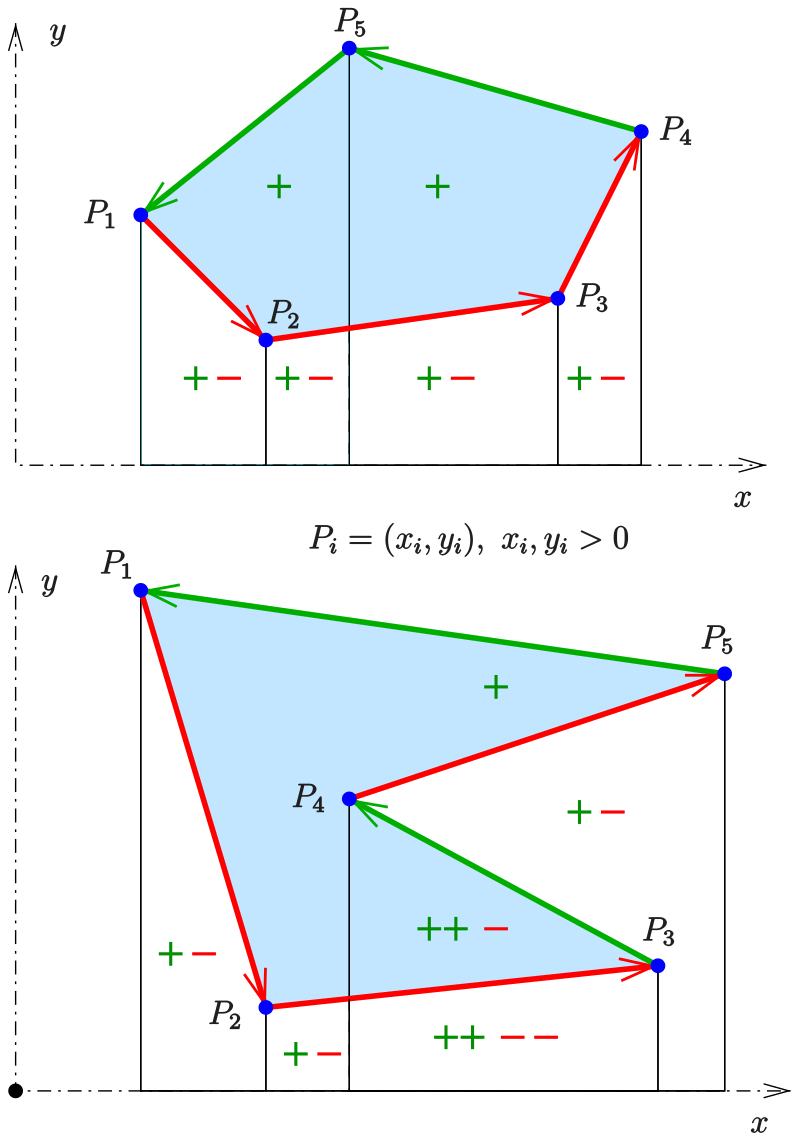
\includegraphics[width=6cm]{shoelace}
    \caption{Deriving the trapezoid formula. Source: Wikipediat{\tt/}shoelace formula.}
\end{figure}
In the 1st case the trapezoid is called {\it negative} in the 2nd case {\it positive}. The negative trapezoids delete those parts of positive trapezoids, which are outside the polygon. In case of a convex polygon (in the diagram the upper example) this is obvious: The polygon area is the sum of the areas of the positive trapezoids (green edges) minus the areas of the negative trapezoids (red edges). In the nonconvex case one has to consider the situation more carefully. In any case the result is 
\begin{equation*}
    A= \sum_{i=1}^n A_i = \frac{1}{2}\sum_{i=1}^n (y_i + y_{i+1})(x_i - x_{i+1}).
\end{equation*}

%------------------------------------------------------------------------------%

\subsubsection{Triangle formula, determinant form -- Công thức tam giác, dạng định thức}
The triangle formula sums up the oriented areas $A_i$ of triangles $OP_iP_{i+1}$:
\begin{equation*}
    A = \frac{1}{2}\sum_{i=1}^n (x_iy_{i+1} - x_{i+1}y_i) = \frac{1}{2}\sum_{i=1}^n \begin{vmatrix}
        x_i & x_{i+1}\\y_i & y_{i+1}
    \end{vmatrix} = \frac{1}{2}\sum_{i=1}^n \begin{vmatrix}
        x_i & y_i\\x_{i+1} & y_{i+1}
    \end{vmatrix} = \frac{1}{2}(x_1y_2 - x_2y_1 + x_2y_3 - x_3y_2 + \cdots + x_ny_1 - x_1y_n).
\end{equation*}
Eliminating the brackets \& using $\sum_{i=1}^n x_iy_i = \sum_{i=1}^n x_{i+1}y_{i+1}$ (convention $P_{n+1} = P_1$), one gets the {\it determinant form} of the area formula:
\begin{equation*}
    A = \frac{1}{2}\sum_{i=1}^n (x_iy_{i+1} - x_{i+1}y_i) = \frac{1}{2}\sum_{i=1}^n \begin{vmatrix}
        x_i & x_{i+1}\\y_i & y_{i+1}
    \end{vmatrix}.
\end{equation*}
Because 1 half of the $i$th determinant is the oriented \href{https://en.wikipedia.org/wiki/Triangle_area}{area of the triangle} $\Delta OP_iP_{i+1}$ this version of the area formula is called {\it triangle form}.

-- Công thức tam giác tổng hợp các diện tích định hướng $A_i$ của các tam giác $OP_iP_{i+1}$:
\begin{equation*}
    A = \frac{1}{2}\sum_{i=1}^n (x_iy_{i+1} - x_{i+1}y_i) = \frac{1}{2}\sum_{i=1}^n \begin{vmatrix}
        x_i & x_{i+1}\\y_i & y_{i+1}
    \end{vmatrix} = \frac{1}{2}\sum_{i=1}^n \begin{vmatrix}
        x_i & y_i\\x_{i+1} & y_{i+1}
    \end{vmatrix} = \frac{1}{2}(x_1y_2 - x_2y_1 + x_2y_3 - x_3y_2 + \cdots + x_ny_1 - x_1y_n).
\end{equation*}
Loại bỏ dấu ngoặc \& sử dụng $\sum_{i=1}^n x_iy_i = \sum_{i=1}^n x_{i+1}y_{i+1}$ (quy ước $P_{n+1} = P_1$), ta sẽ có được {\it dạng định thức} của công thức diện tích:
\begin{equation*}
    A = \frac{1}{2}\sum_{i=1}^n (x_iy_{i+1} - x_{i+1}y_i) = \frac{1}{2}\sum_{i=1}^n \begin{vmatrix}
        x_i & x_{i+1}\\y_i & y_{i+1}
    \end{vmatrix}.    
\end{equation*}
Vì 1 nửa của định thức $i$ là diện tích định hướng của tam giác $OP_iP_{i+1}$ nên phiên bản này của công thức diện tích được gọi là {\it dạng tam giác}.

%------------------------------------------------------------------------------%

\subsubsection{Shoelace formula -- Công thức dây giày}
The triangle formula is the base of the popular {\it shoelace formula}, which is a scheme that optimizes the calculation of the sum of the $2\times2$-determinants by hand:
\begin{equation*}
    2A = \begin{vmatrix}
        x_1 & x_2\\y_1 & y_2
    \end{vmatrix} + \begin{vmatrix}
        x_2 & x_3\\y_2 & y_3
    \end{vmatrix} + \cdots + \begin{vmatrix}
        x_n & x_1\\y_n & y_1
    \end{vmatrix} = \begin{vmatrix}
        x_1 & x_2 & x_3 & \cdots & x_n & x_1\\y_1 & y_2 & y_3 & \cdots & y_n & y_1\\
    \end{vmatrix}
\end{equation*}
Sometimes this determinant is transposed (written vertically, in 2 columns).

%------------------------------------------------------------------------------%

\subsubsection{Other formulas}

\begin{equation*}
    A = \frac{1}{2}\sum_{i=1}^n y_i(x_{i-1} - x_{i+1}) = \frac{1}{2}\left(y_1(x_n - x_2) + y_2(x_1 - x_3) + \cdots + y_n(x_{n-1} - x_1)\right) = \frac{1}{2}\sum_{i=1}^n x_i(y_{i+1} - y_{i-1}).
\end{equation*}
With $\sum_{i=1}^n x_iy_{i+1} = \sum_{i=1}^n x_{i-1}y_i$ (convention $P_0 = P_n,P_{n+1} = P_1$) one gets
\begin{equation*}
    2A = \sum_{i=1}^n (x_iy_{i+1} - x_{i+1}y_i) = \sum_{i=1}^n x_iy_{i+1} - \sum_{i=1}^n x_{i+1}y_i = \sum_{i=1}^n x_{i-1}y_i - \sum_{i=1}^n x_{i+1}y_i.
\end{equation*}
Combining both sums \& excluding $y_i$ leads to
\begin{equation*}
    A = \frac{1}{2}\sum_{i=1}^n y_i(x_{i-1} - x_{i+1}).
\end{equation*}
With the identity $\sum_{i=1}^n x_{i+1}y_i = \sum_{i=1}^n x_iy_{i-1}$ one gets
\begin{equation*}
    A = \frac{1}{2}\sum_{i=1}^n x_i(y_{i+1} - y_{i-1}).
\end{equation*}
Alternatively, this is a special case of Green's theorem with 1 function set to 0 \& the other set to $x$, s.t. the area is the integral of $x\,{\rm d}y$ along the boundary.

-- Với $\sum_{i=1}^n x_iy_{i+1} = \sum_{i=1}^n x_{i-1}y_i$ (quy ước $P_0 = P_n,P_{n+1} = P_1$) ta có
\begin{equation*}
    2A = \sum_{i=1}^n (x_iy_{i+1} - x_{i+1}y_i) = \sum_{i=1}^n x_iy_{i+1} - \sum_{i=1}^n x_{i+1}y_i = \sum_{i=1}^n x_{i-1}y_i - \sum_{i=1}^n x_{i+1}y_i.
\end{equation*}
Kết hợp cả 2 tổng \& loại trừ $y_i$ dẫn đến
\begin{equation*}
    A = \frac{1}{2}\sum_{i=1}^n y_i(x_{i-1} - x_{i+1}).
\end{equation*}
Với hằng đẳng thức $\sum_{i=1}^n x_{i+1}y_i = \sum_{i=1}^n x_iy_{i-1}$ ta có
\begin{equation*}
    A = \frac{1}{2}\sum_{i=1}^n x_i(y_{i+1} - y_{i-1}).
\end{equation*}
Ngoài ra, đây là trường hợp đặc biệt của định lý Green với 1 hàm được đặt thành 0 \& hàm còn lại được đặt thành $x$, s.t. diện tích là tích phân của $x\,{\rm d}y$ dọc theo biên.

%------------------------------------------------------------------------------%

\subsubsection{Exterior algebra -- Đại số ngoài}
A particularly concise statement of the formula can be given in terms of the exterior algebra. Let ${\bf v}_1,{\bf v}_2,\ldots,{\bf v}_n$ be the consecutive vertices of the polygon. The Cartesian coordinate expansion of the outer product w.r.t. the standard ordered orthonormal plane basis $({\bf x},{\bf y})$ gives ${\bf v}_i\land{\bf v}_{i+1} = (x_iy_{i+1} - x_{i+1}y_i){\bf x}\land{\bf y}$ \& the oriented area is given as follows:
\begin{equation*}
    A = \frac{1}{2}\sum_{i=1}^n {\bf v}_i\land{\bf v}_{i+1} = \frac{1}{2}\sum_{i=1}^n (x_iy_{i+1} - x_{i+1}y_i){\bf x}\land{\bf y}.
\end{equation*}
The area is given as a multiple of the unit area ${\bf x}\land{\bf y}$.

-- 1 phát biểu đặc biệt ngắn gọn về công thức có thể được đưa ra dưới dạng đại số ngoài. Giả sử ${\bf v}_1,{\bf v}_2,\ldots,{\bf v}_n$ là các đỉnh liên tiếp của đa giác. Khai triển tọa độ Descartes của tích ngoài w.r.t. cơ sở mặt phẳng chuẩn trực chuẩn sắp xếp $({\bf x},{\bf y})$ cho ${\bf v}_i\land{\bf v}_{i+1} = (x_iy_{i+1} - x_{i+1}y_i){\bf x}\land{\bf y}$ \& diện tích định hướng được đưa ra như sau:
\begin{equation*}
    A = \frac{1}{2}\sum_{i=1}^n {\bf v}_i\land{\bf v}_{i+1} = \frac{1}{2}\sum_{i=1}^n (x_iy_{i+1} - x_{i+1}y_i){\bf x}\land{\bf y}.
\end{equation*}
Diện tích được đưa ra dưới dạng bội số của diện tích đơn vị ${\bf x}\land{\bf y}$.

\begin{baitoan}[Area of polygon -- Diện tích đa giác]
    Viết thuật toán \& chương trình {\sf C{\tt/}C++, Pascal, Python} để tính diện tích của đa giác $n\in\mathbb{N},n\ge3$ đỉnh $A_1A_2\ldots A_n$ với tọa độ $n$ đỉnh $A_i(x_i,y_i)\in\mathbb{R}^2$ cho trước, $\forall i\in[n]$c.
    \item {\sf Input.} Dòng 1 chứa 1 số nguyên $n\in\mathbb{N},n\ge3$. Mỗi dòng trong $n$ dòng tiếp theo chứa 2 số thực $x_i,y_i\in\mathbb{R}$, $\forall i\in[n]$.
    \item {\sf Output.} In ra 1 số thực dương là diện tích của đa giác $A_1A_2\ldots A_n$.
\end{baitoan}

%------------------------------------------------------------------------------%

\subsection{Manipulations of a polygon -- Các thao tác trên 1 đa giác}
$A(P_1,\ldots,P_n)$ indicates the oriented area of the simple polygon $P_1,\ldots,P_n$ with $n\in\mathbb{N},n\ge4$. $A$ is positive{\tt/}negative if the orientation of the polygon is positive{\tt/}negative. From the triangle form of the area formula or the diagram below one observes for $i\in\overline{2,n-1}$:
\begin{equation*}
    A(P_1,\ldots,P_n) = A(P_1,\ldots,P_{i-1},P_{i+1},\ldots,P_n) + A(P_{i-1},P_i,P_{i+1}).
\end{equation*}
In case of $i = 1$ or $i = n$ one should 1st shift the indices. Hence:
\begin{enumerate}
    \item Moving $P_i$ affects only $A(P_{i-1},P_i,P_{i+1})$ \& leaves $A(P_1,\ldots,P_{i-1},P_{i+1},\ldots,P_n)$ unchanged. There is no change of the area if $P_i$ is moved parallel to $\overline{P_{i-1}P_{i+1}}$.
    \item Purging $P_i$ changes the total area by $A(P_{i-1},P_i,P_{i+1})$, which can be positive or negative.
    \item Inserting point $Q$ between $P_i,P_{i+1}$ changes the total area by $A(P_i,Q,P_{i+1})$, which can be positive or negative.
\end{enumerate}
-- $A(P_1,\ldots,P_n)$ biểu thị diện tích định hướng của đa giác đơn $P_1,\ldots,P_n$ với $n\in\mathbb{N},n\ge4$. $A$ là dương{\tt/}âm nếu định hướng của đa giác là dương{\tt/}âm. Từ dạng tam giác của công thức diện tích hoặc sơ đồ bên dưới, người ta quan sát thấy đối với $i\in\overline{2,n-1}$:
\begin{equation*}
    A(P_1,\ldots,P_n) = A(P_1,\ldots,P_{i-1},P_{i+1},\ldots,P_n) + A(P_{i-1},P_i,P_{i+1}).
\end{equation*}
Trong trường hợp $i = 1$ hoặc $i = n$, trước tiên người ta phải dịch chuyển các chỉ số. Do đó:
\begin{enumerate}
    \item Di chuyển $P_i$ chỉ ảnh hưởng đến $A(P_{i-1},P_i,P_{i+1})$ \& giữ nguyên $A(P_1,\ldots,P_{i-1},P_{i+1},\ldots,P_n)$. Không có thay đổi nào về diện tích nếu $P_i$ được di chuyển song song với $\overline{P_{i-1}P_{i+1}}$.
    \item Xóa $P_i$ làm thay đổi tổng diện tích theo $A(P_{i-1},P_i,P_{i+1})$, có thể dương hoặc âm.
    \item Chèn điểm $Q$ giữa $P_i,P_{i+1}$ làm thay đổi tổng diện tích theo $A(P_i,Q,P_{i+1})$, có thể dương hoặc âm.
\end{enumerate}


%------------------------------------------------------------------------------%

\subsection{Generalization of shoelace formula}
In higher dimensions the area of a polygon can be calculated from its vertices using the exterior algebra form of the Shoelace formula (e.g., in 3D, the sum of successive \href{https://en.wikipedia.org/wiki/Cross_product}{cross products}):
\begin{equation*}
    A = \frac{1}{2}\left\|\sum_{i=1}^n v_i\land v_{i+1}\right\|
\end{equation*}
(when the vertices are not \href{https://en.wikipedia.org/wiki/Coplanarity}{coplanar} this computes the \href{https://en.wikipedia.org/wiki/Vector_area}{vector area} enclosed by the loop, i.e., the \href{https://en.wikipedia.org/wiki/Projected_area}{projected area} or ``shadow'' in the plane in which it is greatest).

-- Ở các chiều cao hơn, diện tích của 1 đa giác có thể được tính từ các đỉnh của nó bằng cách sử dụng dạng đại số ngoài của công thức Shoelace (ví dụ, trong 3D, tổng của các tích có hướng liên tiếp):
\begin{equation*}
    A = \frac{1}{2}\left\|\sum_{i=1}^n v_i\land v_{i+1}\right\|
\end{equation*}
(khi các đỉnh không đồng phẳng, công thức này sẽ tính diện tích vectơ được bao quanh bởi vòng lặp, tức là diện tích chiếu hoặc ``bóng'' trên mặt phẳng mà diện tích đó lớn nhất).

This formulation can also be generalized to calculate the volume of an $n$-dimensional polytope from the coordinates of its vertices, or more accurately, from its hypersurface mesh. E.g., the volume of a 3D polyhedron can be found by triangulating its surface mesh \& summing the signed volumes of the tetrahedra formed by each surface triangle \& the origin:
\begin{equation*}
    V = \frac{1}{6}\left\|\sum_F v_a\land v_b\land v_c\right\|
\end{equation*}
where the sum is over the faces \& care has to be taken to order the vertices consistently (all clockwise or anticlockwise viewed from outside the polyhedron). Alternatively, an expression in terms of the face areas \& surface normals may be derived using the divergence theorem.

-- Công thức này cũng có thể được khái quát hóa để tính thể tích của 1 đa diện $n$ chiều từ tọa độ các đỉnh của nó, hoặc chính xác hơn, từ lưới siêu bề mặt của nó. E.g., thể tích của 1 đa diện 3D có thể được tìm thấy bằng cách tam giác hóa lưới bề mặt của nó \& cộng các thể tích có dấu của tứ diện được tạo thành bởi mỗi tam giác bề mặt \& gốc:
\begin{equation*}
    V = \frac{1}{6}\left\|\sum_F v_a\land v_b\land v_c\right\|
\end{equation*}
trong đó tổng nằm trên các mặt \& phải cẩn thận để sắp xếp các đỉnh 1 cách nhất quán (tất cả theo chiều kim đồng hồ hoặc ngược chiều kim đồng hồ khi nhìn từ bên ngoài đa diện). Ngoài ra, 1 biểu thức theo diện tích mặt \& pháp tuyến bề mặt có thể được suy ra bằng cách sử dụng định lý phân kỳ.

%------------------------------------------------------------------------------%

\section{Problems: Computational elementary geometry}

\begin{baitoan}[Bao phủ hình chữ nhật nguyên 2D nhỏ nhất]
    {\rm(2.5 điểm)} Viết chương trình Python để tính chu vi, diện tích, \& độ dài đường chéo hình chữ nhật nhỏ nhất ``chứa trọn'' $n\in\mathbb{N}^\star$ điểm $A_1(x_1,y_1),A_2(x_2,y_2)$, $\ldots,A_n(x_n,y_n)\in\mathbb{R}^2$ với tọa độ nguyên $x_i,y_i\in\mathbb{Z}$, $\forall i = 1,\ldots,n$, cho trước trong mặt phẳng 2 chiều, ``chứa trọn'' ở đây nghĩa là các điểm chỉ được nằm bên trong hình chữ nhật, không được nằm trên cạnh hình chữ nhật.
    \item {\sf Input.} Dòng 1 chứa số nguyên $n\in\mathbb{N}^\star$:  * số điểm trong mặt phẳng 2 chiều. $n$ dòng tiếp theo, mỗi dòng chứa 2 số nguyên $x_i,y_i\in\mathbb{Z}$: hoành độ \& tung độ của điểm thứ $i$ $A_i(x_i,y_i)$.
    \item {\sf Output.} In ra chu vi, diện tích, \& đường chéo của hình chữ nhật thỏa mãn nhờ gọi lại hàm của Bài 1 (hoặc tự viết lại nếu muốn).
    \item {\sf Sample.}
    \begin{table}[H]
        \centering
        \begin{tabular}{|l|l|}
            \hline
            \verb|min_rectangle.inp| & \verb|min_rectangle.out| \\
            \hline
            4 & $P = 26$ \\
            1 0 & $S = 40$ \\
            -2 2 & $d = 9.43398113206$ \\
            -1 3 & \\
            4 2 & \\
            \hline
        \end{tabular}
    \end{table}
\end{baitoan}

\begin{proof}[Solution]
    Python:
    \begin{Verbatim}[numbers=left,xleftmargin=5mm]
        n = int(input()) # number of 2D points -- số điểm trên mặt phẳng
        x_min = y_min = 1e9
        x_max = y_max = -1e9
        for i in range(n):
        x, y = map(int, input().split())
        if x < x_min:
        x_min = x
        if x > x_max:
        x_max = x
        if y < y_min:
        y_min = y
        if y > y_max:
        y_max = y
        a, b = x_max - x_min + 2, y_max - y_min + 2
        print('P =', 2 * (a + b))
        print('S =', a * b)
        print('d =', sqrt(a * a + b * b))
    \end{Verbatim}
\end{proof}

\begin{baitoan}[Bao phủ hình hộp chữ nhật nguyên 3D nhỏ nhất]
    {\rm(3.5 điểm)} Viết chương trình Python để tính diện tích toàn phần, thể tích, \& độ dài đường chéo hình hộp chữ nhật nhỏ nhất chứa $n\in\mathbb{N}^\star$ điểm $A_1(x_1,y_1,z_1),A_2(x_2,y_2,z_2)$, $\ldots,A_n(x_n,y_n,z_n)\in\mathbb{R}^3$ với tọa độ nguyên $x_i,y_i\in\mathbb{Z}$, $\forall i = 1,\ldots,n$, cho trước trong không gian 3 chiều, ở đây các điểm có thể nằm bên trong hoặc nằm trên cạnh hình hộp chữ nhật.
    \item {\sf Input.} Dòng 1 chứa số nguyên $n\in\mathbb{N}^\star$: số điểm trong không gian 3 chiều. $n$ dòng tiếp theo, mỗi dòng chứa 3 số nguyên $x_i,y_i,z_i\in\mathbb{Z}$: hoành độ, tung độ, \& cao độ của điểm thứ $i$ $A_i(x_i,y_i,z_i)$.
    \item {\sf Output.} In ra diện tích toàn phần, thể tích, \& độ dài đường chéo hình hộp chữ nhật thỏa mãn, biết với hình hộp chữ nhật có kích thước $a\times b\times c$ thì $S_{\rm tp} = 2(ab + bc + ca),V = abc,d = \sqrt{a^2 + b^2 + c^2}$.
    \item {\sf Sample.}
    \begin{table}[H]
        \centering
        \begin{tabular}{|l|l|}
            \hline
            \verb|min_rectangular_cuboid.inp| & \verb|min_rectangular_cuboid.out| \\
            \hline
            4 & $S_{\rm tp} = 22$ \\
            1 0 0& $V = 6$ \\
            0 1 0 & $d = 3.74165738677 $ \\
            -1 0 2 & \\
            2 0 1 & \\
            \hline
        \end{tabular}
    \end{table}
\end{baitoan}

\begin{proof}[Solution]
    Python:
    \begin{Verbatim}[numbers=left,xleftmargin=5mm]
        n = int(input()) # number of 3D points
        x_min = y_min = z_min = 1e9
        x_max = y_max = z_max = -1e9
        for i in range(n):
        x, y, z = map(int, input().split())
        if x < x_min:
        x_min = x
        if x > x_max:
        x_max = x
        if y < y_min:
        y_min = y
        if y > y_max:
        y_max = y
        if z < z_min:
        z_min = z
        if z > z_max:
        z_max = z
        a, b, c = x_max - x_min, y_max - y_min, z_max - z_min
        print('S_tp =', 2 * (a * b + b * c + c * a))
        print('V =', a * b * c)
        print('d =', sqrt(a * a + b * b + c * c))
    \end{Verbatim}
\end{proof}

\begin{baitoan}[\cite{TL_chuyen_Tin_quyen_3}, 8.1, segment in triangle -- tìm độ dài đoạn thẳng nằm trong tam giác]
    Trên mặt phẳng cho $\Delta ABC$ \& đoạn thẳng $DE$. Tính độ dài của phần đoạn thẳng $DE$ nằm trong $\Delta ABC$.
    \item {\sf Input.} Dòng 1 có $6$ số thực $x_A,y_A,x_B,y_B,x_C,y_C$ lần lượt từng cặp là tọa độ tương ứng của 3 đỉnh $A,B,C$. Dòng 2 là $4$ số thực $x_D,y_D,x_E,y_E$ lần lượt từng cặp là tọa độ 2 điểm $D,E$.
    \item {\sf Output.} In 1 số thực duy nhất là độ dài phần đoạn thẳng $DE$ nằm trong $\Delta ABC$.
    \item {\sf Sample.}
    \begin{table}[H]
        \centering
        \begin{tabular}{|l|l|}
            \hline
            \verb|segment_in_triangle.inp| & \verb|segment_in_triangle.out| \\
            \hline
            0 2 2 4 4 2 & 3.16228 \\
            0 2 3 3 & \\
            \hline
        \end{tabular}
    \end{table}
\end{baitoan}

\begin{baitoan}[\cite{TL_chuyen_Tin_quyen_3}, 8.2, common area of 2 triangles -- tìm diện tích phần chung của 2 tam giác]
    Trên mặt phẳng cho $2$ tam giác. Tìm diện tích phần chung của $2$ tam giác.
    \item {\sf Input.} Gồm 2 dòng, mỗi dòng có $6$ số thực lần lượt từng cặp là tọa độ tương ứng của $3$ đỉnh của 1 tam giác. Các tọa độ có giá trị tuyệt đối $\le10^3$.
    \item {\sf Output.} In ra duy nhất 1 số thực là diện tích phần chung của 2 tam gaics này.  
    \item {\sf Constraints.} $n\in[2\cdot10^5],m\in[100],x_i\in\{0,1,\ldots,m\}$.
    \item {\sf Sample.}
    \begin{table}[H]
        \centering
        \begin{tabular}{|l|l|}
            \hline
            \verb|common_area_triangle.inp| & \verb|common_area_triangle.out| \\
            \hline
            0 6 8 6 4 0 & 16 \\
            4 8 8 2 0 2 & \\
            \hline
        \end{tabular}
    \end{table}
\end{baitoan}

\begin{problem}[\href{https://cses.fi/problemset/task/2189}{CSES Problem Set{\tt/}point location test}]
    There is a line that goes through the points $p_1 = (x_1,y_2),p_2(x_2,y_2)$. There is also a point $p_3 = (x_3,y_3)$. Determine whether $p_3$ is located on the left or right side of the line or if it touches the line when we are looking from $p_1$ to $p_2$.
    \item {\sf Input.} The 1st input line has an integer $t\in\mathbb{N}^\star$: the number of tests. After this, there are $t$ lines that describe the tests. Each line has $6$ integers $x_1,y_1,x_2,y_2,x_3,y_3\in\mathbb{Z}$.
    \item {\sf Output.} For each test, print {\tt LEFT, RIGHT} or {\tt TOUCH}.
    \item {\sf Constraints.} $t\in[10^5],x_i,y_i\in\overline{-10^9,10^9}$, $\forall i\in[3]$, $x_1\ne x_2$ or $y_1\ne y_2$ (i.e., $(x_1,x_1)\ne(x_2,y_2)$).
    \item {\sf Sample.}
    \begin{table}[H]
        \centering
        \begin{tabular}{|l|l|}
            \hline
            \verb|point_location_test.inp| & \verb|point_location_test.out| \\
            \hline
            3 & LEFT \\
            1 1 5 3 2 3 0 2 & RIGHT \\
            1 1 5 3 4 1 & TOUCH \\
            1 1 5 3 3 2 & \\
            \hline
        \end{tabular}
    \end{table}
\end{problem}

\begin{proof}[Solution]
    C++:
    \begin{enumerate}
        \item PVT's C++: point location test
        \begin{Verbatim}[numbers=left,xleftmargin=5mm]
#include <bits/stdc++.h>
using namespace std;
#define ll long long

void solve() {
    ll x1, y1, x2, y2, x3, y3;
    cin >> x1 >> y1 >> x2 >> y2 >> x3 >> y3;
    ll dot = (x2 - x1) * (x3 - x1) + (y2 - y1) * (y3 - y1);
    ll det = (x2 - x1) * (y3 - y1) - (x3 - x1) * (y2 - y1);
    double angle = atan2(det, dot);
    if (angle == 0 || angle == M_PI || angle == -M_PI) cout << "TOUCH\n";
    else if (angle > 0) cout << "LEFT\n";
    else cout << "RIGHT\n";
}

int main() {
    ios_base::sync_with_stdio(false); cin.tie(NULL);
    ll t; cin >> t;
    while (t--)
    solve();
}
        \end{Verbatim}
        \item NHT's C++: point location test
        \begin{Verbatim}[numbers=left,xleftmargin=5mm]
#include <bits/stdc++.h>
#define ll long long
using namespace std;

int t;

int main() {
    ios_base::sync_with_stdio(false);
    cin.tie(nullptr);
    
    cin >> t;
    while (t--) {
        ll x1, y1, x2, y2, x3, y3;
        cin >> x1 >> y1 >> x2 >> y2 >> x3 >> y3;
        ll area = (x2 - x1) * (y3 - y1) - (y2 - y1) * (x3 - x1);
        if (area > 0)
        cout << "LEFT\n";
        else if (area < 0)
        cout << "RIGHT\n";
        else
        cout << "TOUCH\n";
    }
}
        \end{Verbatim}
    \end{enumerate}
\end{proof}

\begin{problem}[\href{https://cses.fi/problemset/task/2190}{CSES Problem Set{\tt/}line segment intersection}]
    There are $2$ line segments: the 1st goes through the points $(x_1,y_1),(x_2,y_2)$, \& the 2nd goes through the points $(x_3,y_3),(x_4,y_4)$. Determine if the line segments intersect, i.e., they have at least $1$ common point.
    \item {\sf Input.} The 1st input line has an integer $t\in\mathbb{N}^\star$: the number of tests. After this, there are $t$ lines that describe the tests. Each line has $8$ integers $x_1,y_1,x_2,y_2,x_3,y_3,x_4,y_4\in\mathbb{Z}$.
    \item {\sf Output.} For each test, print {\tt TEST} if the line segments intersect \& {\tt NO} otherwise.
    \item {\sf Constraints.} $t\in[10^5],x_i,y_i\in\overline{-10^9,10^9}$, $\forall i\in[4]$, $(x_1,x_1)\ne(x_2,y_2)$, $(x_3,x_3)\ne(x_4,y_4)$.
    \item {\sf Sample.}
    \begin{table}[H]
        \centering
        \begin{tabular}{|l|l|}
            \hline
            \verb|line_segment_intersection.inp| & \verb|line_segment_intersection.out| \\
            \hline
            5 & NO \\
            1 1 5 3 1 2 4 3 & YES \\
            1 1 5 3 1 1 4 3 & YES \\
            1 1 5 3 2 3 4 1 & YES \\
            1 1 5 3 2 4 4 1 & YES \\
            1 1 5 3 3 2 7 4 & \\
            \hline
        \end{tabular}
    \end{table}
\end{problem}

\begin{proof}[Solution]
    C++:
    \begin{enumerate}
        \item VNTA's C++: line segment intersection: \url{https://github.com/NQBH/advanced_STEM_beyond/blob/main/OLP_ICPC/C%2B%2B/VNTA_line_segment_intersection.cpp}.
        \begin{Verbatim}[numbers=left,xleftmargin=5mm]
#include <bits/stdc++.h>
using namespace std;
#define ll long long

struct P {
    ll x;
    ll y;
};

int ori(P a, P b, P c) {
    ll v = (b.y - a.y) * (c.x - b.x) - (b.x - a.x) * (c.y - b.y);
    if (v == 0) return 0;
    return (v > 0) ? 1 : 2;
}

bool onSeg(P a, P b, P c) {
    return (b.x <= max(a.x, c.x) &&
    b.x >= min(a.x, c.x) &&
    b.y <= max(a.y, c.y) &&
    b.y >= min(a.y, c.y));
}

bool check(P a, P b, P c, P d) {
    int o1 = ori(a, b, c);
    int o2 = ori(a, b, d);
    int o3 = ori(c, d, a);
    int o4 = ori(c, d, b);
    
    if (o1 != o2 && o3 != o4) return true;
    
    if (o1 == 0 && onSeg(a, c, b)) return true;
    if (o2 == 0 && onSeg(a, d, b)) return true;
    if (o3 == 0 && onSeg(c, a, d)) return true;
    if (o4 == 0 && onSeg(c, b, d)) return true;
    
    return false;
}

int main() {
    ios::sync_with_stdio(0);
    cin.tie(0);
    
    int t; cin >> t;
    while (t--) {
        P p1, p2, p3, p4;
        cin >> p1.x >> p1.y >> p2.x >> p2.y >> p3.x >> p3.y >> p4.x >> p4.y;
        if (check(p1, p2, p3, p4)) cout << "YES\n";
        else cout << "NO\n";
    }
}
        \end{Verbatim}
    \end{enumerate}
\end{proof}

\begin{problem}[\href{https://cses.fi/problemset/task/2191}{CSES Problem Set{\tt/}polygon area}]
    Calculate the area of a given polygon. The polygon consists of $n$ vertices $(x_i,y_i)$, $\forall i\in[n]$. The vertices $(x_i,y_i)$ \& $(x_{i+1},y_{i+1})$ are adjacent for $i\in[n - 1]$, \& the vertices $(x_1,y_1)$ \& $(x_n,y_n)$ are also adjacent.
    \item {\sf Input.} The 1st input line has an integer $n\in\mathbb{N}^\star$: the number of vertices. After this, there are $n$ lines that describe the vertices. The $i$th such line has $2$ integers $x_i,y_i\in\mathbb{Z}$. You may assume that the polygon is simple, i.e., it does not intersect itself.
    \item {\sf Output.} Print $1$ integer: $2a\in\mathbb{Z}$ where the area of the polygon is $a$ (is ensures that the result is an integer).
    \item {\sf Constraints.} $n\in\overline{3,1000},x_i,y_i\in\overline{-10^9,10^9}$, $\forall i\in[n]$.
    \item {\sf Sample.}
    \begin{table}[H]
        \centering
        \begin{tabular}{|l|l|}
            \hline
            \verb|polygon_area.inp| & \verb|polygon_area.out| \\
            \hline
            4 & 16 \\
            1 1 & \\
            4 2 & \\
            3 5 & \\
            1 4 & \\
            \hline
        \end{tabular}
    \end{table}
\end{problem}

\begin{problem}[\href{https://cses.fi/problemset/task/2192}{CSES Problem Set{\tt/}point in polygon}]
    You are given a polygon of $n\in\mathbb{N}^\star$ vertices \& a list of $m\in\mathbb{N}^\star$ points. Determine for each point if it is inside, outside or on the boundary of the polygon. The polygon consists of $n$ vertices $(x_i,y_i)$, $\forall i\in[n]$. The vertices $(x_i,y_i)$ \& $(x_{i+1},y_{i+1})$ are adjacent for $i\in[n - 1]$, \& the vertices $(x_1,y_1)$ \& $(x_n,y_n)$ are also adjacent.
    \item {\sf Input.} The 1st input line has $2$ integer $n,m\in\mathbb{N}^\star$: the number of vertices in the polygon \& the number of points. After this, there are $n$ lines that describe the polygon. The $i$th such line has $2$ integers $x_i,y_i$. You may assume that the polygon is simple, i.e., it does not intersect itself. Finally, there are $m$ lines that describe the points. Each line has $2$ integers $x,y\in\mathbb{Z}$.
    \item {\sf Output.} For each point, print {\tt INSIDE, OUTSIDE} or {\tt BOUNDARY}.
    \item {\sf Constraints.} $M,n\in\overline{3,1000},m\in[1000],x,y,x_i,y_i\in\overline{-10^9,10^9}$, $\forall i\in[n]$.
    \item {\sf Sample.}
    \begin{table}[H]
        \centering
        \begin{tabular}{|l|l|}
            \hline
            \verb|point_in_polygon.inp| & \verb|point_in_polygon.out| \\
            \hline
            4 3 & INSIDE \\
            1 1 & OUTSIDE \\
            4 2 & BOUNDARY \\
            3 5 & \\
            1 4 & \\
            2 3 & \\
            3 1 & \\
            1 3 & \\
            \hline
        \end{tabular}
    \end{table}
\end{problem}

\begin{problem}[\href{https://cses.fi/problemset/task/2193}{CSES Problem Set{\tt/}polygon lattice points}]
    Given a polygon , calculate the number of lattice points inside the polygon \& on its boundary. A {\rm lattice point} is a point whose coordinates are integers. The polygon consists of $n\in\mathbb{N}^\star$ vertices $(x_i,y_i)$, $\forall i\in[n]$. The vertices $(x_i,y_i)$ \& $(x_{i+1},y_{i+1})$ are adjacent for $i\in[n - 1]$, \& the vertices $(x_1,y_1)$ \& $(x_n,y_n)$ are also adjacent.
    \item {\sf Input.} The 1st input line has an integer $n\in\mathbb{N}^\star$:  the number of vertices. After this, there are $n$ lines that describe the vertices. The $i$th such line has $2$ integers $x_i,y_i$. You may assume that the polygon is simple, i.e., it does not intersect itself.
    \item {\sf Output.} Print $2$ integers: the number of lattice points inside the polygon \& on its boundary.
    \item {\sf Constraints.} $n\in\overline{3,10^5},x_i,y_i\in\overline{-10^9,10^9}$, $\forall i\in[n]$.
    \item {\sf Sample.}
    \begin{table}[H]
        \centering
        \begin{tabular}{|l|l|}
            \hline
            \verb|polygon_lattice_point.inp| & \verb|polygon_lattice_point.out| \\
            \hline
            4 & 6 8 \\
            1 1 & \\
            5 3 & \\
            3 5 & \\
            1 4 & \\
            \hline
        \end{tabular}
    \end{table}
\end{problem}

\begin{problem}[\href{https://cses.fi/problemset/task/2194}{CSES Problem Set{\tt/}minimum Euclidean distance}]
    Given a set of points in 2D plane, find the minimum Euclidean distance between $2$ distinct points. The Euclidean distance of points $(x_1,y_1),(x_2,y_2)$ is $d((x_1,y_1),(x_2,y_2)) = \sqrt{(x_1 - x_2)^2 + (y_1 - y_2)^2}$.
    \item {\sf Input.} The 1st input line has an integer $n\in\mathbb{N}^\star$: the number of points. After this, there are $n$ lines that describe the points. Each line has $2$ integers $x,y\in\mathbb{Z}$: the coordinates of a point. You may assume that each point is distinct.
    \item {\sf Output.} Print $1$ integer: $d^2$ where $d$ is the minimum Euclidean distance (this ensures that the result is an integer).
    \item {\sf Constraints.} $n\in\overline{2,2\cdot10^5},x,y\in\overline{-10^9,10^9}$.
    \item {\sf Sample.}
    \begin{table}[H]
        \centering
        \begin{tabular}{|l|l|}
            \hline
            \verb|minimum_Euclidean_distance.inp| & \verb|minimum_Euclidean_distance.out| \\
            \hline
            4 & 2 \\
            2 1 & \\
            4 4 & \\
            1 2 & \\
            6 3 & \\
            \hline
        \end{tabular}
    \end{table}
\end{problem}

\begin{problem}[\href{https://cses.fi/problemset/task/2195}{CSES Problem Set{\tt/}convex hull}]
    Given a set of $n\in\mathbb{N}^\star$ points in the 2D plane, determine the convex hull of the points.
    \item {\sf Input.} The 1st input line has an integer $n\in\mathbb{N}^\star$: the number of points.  After this, there are $n$ lines that describe the points. Each line has $2$ integers $x,y\in\mathbb{Z}$: the coordinates of a point. You may assume that each point is distinct, \& the area of the hull is positive.
    \item {\sf Output.} 1st print an integer $k\in\mathbb{N}$: the number of points in the convex hull. After this, print $k$ lines that describe the points. You can print the points in any order. Print all points that lie on the convex hull.
    \item {\sf Constraints.} $n\in\overline{3,2\cdot10^5},x,y\in\overline{-10^9,10^9}$.
    \item {\sf Sample.}
    \begin{table}[H]
        \centering
        \begin{tabular}{|l|l|}
            \hline
            \verb|.inp| & \verb|.out| \\
            \hline
            6 & 4 \\
            2 1 & 2 1 \\
            2 5 & 2 5 \\
            3 3 & 4 4 \\
            4 3 & 6 3 \\
            4 4 & \\
            6 3 & \\
            \hline
        \end{tabular}
    \end{table}
\end{problem}

\begin{problem}[\href{https://cses.fi/problemset/task/3410}{CSES Problem Set{\tt/}maximum Manhattan distance}]
    A set is initially empty \& $n\in\mathbb{N}^\star$ points are added to it. Calculate the maximum Manhattan distance of $2$ points after each addition.
    \item {\sf Input.} The 1st input line has an integer $n\in\mathbb{N}^\star$: the number of points. The following $n$ lines describe the points. Each line has $2$ integers $x,y\in\mathbb{Z}$. You can assume that each point is distinct.
    \item {\sf Output.} After each addition, print the maximum distance.
    \item {\sf Constraints.} $n\in\overline{2,2\cdot10^5},x,y\in\overline{-10^9,10^9}$.
    \item {\sf Sample.}
    \begin{table}[H]
        \centering
        \begin{tabular}{|l|l|}
            \hline
            \verb|maximum_Manhattan_distance.inp| & \verb|maximum_Manhattan_distance.out| \\
            \hline
            5 & 0 \\
            1 1 & 3 \\
            3 2 & 4 \\
            2 4 & 4 \\
            2 1 & 7 \\
            4 5 & \\
            \hline
        \end{tabular}
    \end{table}
\end{problem}

\begin{problem}[\href{https://cses.fi/problemset/task/3411}{CSES Problem Set{\tt/}all Manhattan distances}]
    Given a set of points, calculate the sum of all Manhattan distances between $2$ point pairs.
    \item {\sf Input.} The 1st input line has an integer $n\in\mathbb{N}^\star$: the number of points. The following $n$ lines describe the points. Each line has $2$ integers $x,y\in\mathbb{Z}$. You can assume that each point is distinct.
    \item {\sf Output.} Print the sum of all Manhattan distances.
    \item {\sf Constraints.} $n\in\overline{2,2\cdot10^5},x,y\in\overline{-10^9,10^9}$.
    \item {\sf Sample.}
    \begin{table}[H]
        \centering
        \begin{tabular}{|l|l|}
            \hline
            \verb|all_Manhattan_distance.inp| & \verb|all_Manhattan_distance.out| \\
            \hline
            5 & 36 \\
            1 1 & \\
            3 2 & \\
            2 4 & \\
            2 1 & \\
            4 5 & \\
            \hline
        \end{tabular}
    \end{table}
\end{problem}

\begin{problem}[\href{https://cses.fi/problemset/task/1740}{CSES Problem Set{\tt/}intersection points}]
    Given $n\in\mathbb{N}^\star$ horizontal \& vertical line segments, calculate the number of their intersection points. You can assume that no parallel line segments intersect, \& no endpoint of a line segment is an intersection point.
    \item {\sf Input.} The 1st input line has an integer $n\in\mathbb{N}^\star$: the number of line segments. Then there are $n$ lines describing the line segments. Each line has $4$ integers: $x_1,y_1,x_2,y_2$: a line segment begins at point $(x_1,y_1)$ \& ends at point $(x_2,y_2)$.
    \item {\sf Output.} Print the number of intersection points.
    \item {\sf Constraints.} $n\in[10^5],x_1,x_2,y_1,y_2\in\overline{-10^6,10^6}$, $(x_1,y_1)\ne(x_2,y_2)$.
    \item {\sf Sample.}
    \begin{table}[H]
        \centering
        \begin{tabular}{|l|l|}
            \hline
            \verb|intersection_point.inp| & \verb|intersection_point.out| \\
            \hline
            3 & 2 \\
            2 3 7 3 & \\
            3 1 3 5 & \\
            6 2 6 6 & \\
            \hline
        \end{tabular}
    \end{table}
\end{problem}

\begin{problem}[\href{https://cses.fi/problemset/task/3427}{CSES Problem Set{\tt/}line segments trace I}]
    There are $n\in\mathbb{N}^\star$ line segments whose endpoints have integer coordinates. The left $x$-coordinate of each segment is $0$ \& the right $x$-coordinate is $m\in\mathbb{N}^\star$. The slope of each segment is an integer. For each $x$-coordinate $0,1,\ldots,m$, find the maximum point in any line segment.
    \item {\sf Input.} The 1st input line has $2$ integer $n,m\in\mathbb{N}^\star$: the number of line segments \& the maximum $x$-coordinate. The next $n$ lines describe the line segments. Each line has $2$ integers $y_1,y_2$: there is a line segment between points $(0,y_1)$ \& $(m,y_2)$.
    \item {\sf Output.} Print $m + 1$ integers: the maximum points for $x = 0,1,\ldots,m$.
    \item {\sf Constraints.} $m,n\in[10^5],m\in[100],y_1,y_2\in\overline{0,10^9}$.
    \item {\sf Sample.}
    \begin{table}[H]
        \centering
        \begin{tabular}{|l|l|}
            \hline
            \verb|line_segment_trace_I.inp| & \verb|line_segment_trace_I.out| \\
            \hline
            4 5 & 10 8 6 5 5 6 \\
            1 6 & \\
            7 2 & \\
            5 5 & \\
            10 0 & \\
            \hline
        \end{tabular}
    \end{table}
\end{problem}

\begin{problem}[\href{https://cses.fi/problemset/task/3428}{CSES Problem Set{\tt/}line segments trace II}]
    There are $n\in\mathbb{N}^\star$ line segments whose endpoints have integer coordinates. Each $x$-coordinate is between $0$ \& $m$. The slope of each segment is an integer. For each $x$-coordinate $0,1,\ldots,m$, find the maximum point in any line segment. If there is no segment at some point, the maximum is $-1$.
    \item {\sf Input.} The 1st input line has $2$ integers $n,m\in\mathbb{N}^\star$: the number  of line segments \& the maximum $x$-coordinate. The next $n$ lines describe the line segments. Each line has $4$ integers $x_1,y_1,x_2,y_2$: there is a line segment between points $(x_1,y_1),(x_2,y_2)$.
    \item {\sf Output.} Print $m + 1$ integers: the maximum points for $x = 0,1,\ldots,m$.
    \item {\sf Constraints.} $m,n\in[10^5],0\le x_1 < x_2\le m,y_1,y_2\in\overline{0,10^9}$.
    \item {\sf Sample.}
    \begin{table}[H]
        \centering
        \begin{tabular}{|l|l|}
            \hline
            \verb|line_segment_trace_II.inp| & \verb|line_segment_trace_II.out| \\
            \hline
            4 5 & -1 2 8 6 6 7 \\
            1 1 3 3 & \\
            1 2 4 2 & \\
            2 4 5 7 & \\
            2 8 5 2 & \\
            \hline
        \end{tabular}
    \end{table}
\end{problem}

\begin{problem}[\href{https://cses.fi/problemset/task/3429}{CSES Problem Set{\tt/}lines \& queries I}]
    Efficiently process the following types of queries:
    \begin{enumerate}
        \item Add a line $ax + b$.
        \item Find the maximum point in any line at position $x$.
    \end{enumerate}
    \item {\sf Input.} The 1st input line has an integer $n\in\mathbb{N}^\star$: the number of queries. The following $n$ lines describe the queries. The format of each line is either {\tt1 a b} or {\tt2 x}. You may assume that the 1st query is of type 1.
    \item {\sf Output.} Print the answer for each query of type 2.
    \item {\sf Constraints.} $n\in[2\cdot10^5],a,b\in\overline{-10^9,10^9},x\in\overline{0,10^5}$.
    \item {\sf Sample.}
    \begin{table}[H]
        \centering
        \begin{tabular}{|l|l|}
            \hline
            \verb|line_query_I.inp| & \verb|line_query_I.out| \\
            \hline
            6 & 3 \\
            1 1 2 & 5 \\
            2 1 & 4 \\
            2 3 & 5 \\
            1 0 4 & \\
            2 1 & \\
            2 3 & \\
            \hline
        \end{tabular}
    \end{table}
\end{problem}

\begin{problem}[\href{https://cses.fi/problemset/task/3430}{CSES Problem Set{\tt/}lines \& queries II}]
    Efficiently process the following types of queries:
    \begin{enumerate}
        \item Add a line $ax + b$ that is active in range $[l,r]$.
        \item Find the maximum point in any active line at position $x$.
    \end{enumerate}
    \item {\sf Input.} The 1st input line has an integer $n\in\mathbb{N}^\star$: the number of queries. The following $n$ lines describe the queries. The format of each line is either {\tt1 a b l r} or {\tt2 x}.
    \item {\sf Output.} Print the answer for each query of type 2. If no line is active, print {\tt NO}.
    \item {\sf Constraints.} $n\in[2\cdot10^5],a,b\in\overline{-10^9,10^9},x,l,r\in\overline{0,10^5}$.
    \item {\sf Sample.}
    \begin{table}[H]
        \centering
        \begin{tabular}{|l|l|}
            \hline
            \verb|line_query_II.inp| & \verb|line_query_II.out| \\
            \hline
            6 & 5 \\
            1 1 2 1 3 & NO \\
            2 3 & 5 \\
            2 4 & 4 \\
            1 0 4 1 5 & \\
            2 3 & \\
            2 4 & \\
            \hline
        \end{tabular}
    \end{table}
\end{problem}

\begin{problem}[\href{https://cses.fi/problemset/task/1741}{CSES Problem Set{\tt/}area of rectangles}]
    Given $n\in\mathbb{N}^\star$, determine the total area of their union.
    \item {\sf Input.} The 1st input line has an integer $n\in\mathbb{N}^\star$: the number of rectangles. After that, there are $n$ lines describing the rectangles. Each line has $4$ integers $x_1,y_1,x_2,y_2$: a rectangle begins at point $(x_1,y_1)$ \& ends at point $(x_2,y_2)$.
    \item {\sf Output.} Print the total area covered by the rectangles.
    \item {\sf Constraints.} $n\in[10^5],m\in[100],x_1,x_2,y_1,y_2\in\overline{-10^6,10^6}$.
    \item {\sf Sample.}
    \begin{table}[H]
        \centering
        \begin{tabular}{|l|l|}
            \hline
            \verb|area_rectangle.inp| & \verb|area_rectangle.out| \\
            \hline
            3 & 24 \\
            1 3 4 5 & \\
            3 1 7 4 & \\
            5 3 8 6 & \\
            \hline
        \end{tabular}
    \end{table}
\end{problem}

\begin{problem}[\href{https://cses.fi/problemset/task/1742}{CSES Problem Set{\tt/}robot path}]
    You are given a description of a robot's path. The robot begins at point $(0,0)$ \& performs $n\in\mathbb{N}^\star$ commands. Each command moves the robot some distance up, down, left, or right. The robot will stop when it has performed all commands, or immediately when it returns to a point that it has already visited. Calculate the total distance the robot moves.
    \item {\sf Input.} The 1st input line has an integer $n\in\mathbb{N}^\star$: the number of commands. After that, there are $n$ lines describing the commands. each line has a character $d$ \& an integer $x\in\mathbb{N}^\star$: the robot moves the distance $x$ to the direction $d$. Each direction is {\tt U, D, L, R} (up, down, left, right).
    \item {\sf Output.} Print the total distance the robot moves.
    \item {\sf Constraints.} $n\in[10^5],x\in[10^6]$.
    \item {\sf Sample.}
    \begin{table}[H]
        \centering
        \begin{tabular}{|l|l|}
            \hline
            \verb|robot_path.inp| & \verb|robot_path.out| \\
            \hline
            5 & 9 \\
            U 2 & \\
            R 3 & \\
            D 1 & \\
            L 5 & \\
            U 2 & \\
            \hline
        \end{tabular}
    \end{table}
\end{problem}

\begin{problem}[IMO2007P6]
    Let $n\in\mathbb{N}^\star$. Consider $S = \{(x,y,z);x,y,z\in\overline{0,n},\ x + y + z > 0\}$ as a set of $(n + 1)^3 - 1$ points in 3D space. Determine the smallest possible number of planes, the union of which contains $S$ but does not include $(0,0,0)$.
\end{problem}

\begin{baitoan}[\cite{Vinh_Lu_Olympic_Toan}, 6., p. 10, IMO2007P6]
    Cho $n\in\mathbb{N}^\star$. Xét $S = \{(x,y,z);x,y,z\in\overline{0,n},\ x + y + z > 0\}$ là 1 tập hợp gồm $(n + 1)^3 - 1$ điểm trong không gian $3$-chiều. Xác định số nhỏ nhất có thể các mặt phẳng mà hợp của chúng chứa tất cả các điểm của $S$ nhưng không chứa điểm $(0,0,0)$.
\end{baitoan}

%------------------------------------------------------------------------------%

\chapter{Number Theory -- Lý Thuyết Số}
\minitoc

%------------------------------------------------------------------------------%

\section{Divisor -- Ước Số}

\begin{problem}[IMO2007P5]
    Let $a,b\in\mathbb{N}^\star$. Show that if $4ab - 1|(4a^2 - 1)^2$, then $a = b$.
\end{problem}

\begin{baitoan}[CP version of IMO2007P5]
    Cho $m,n\in\mathbb{N}^\star$. Đếm số phần tử của tập hợp
    \begin{equation*}
        S = \{(a,b)\in[m]\times[n];4ab - 1|(4a^2 - 1)^2\} = \{(a,b)\in[m]\times[n];(4a^2 - 1)^2\divby4ab - 1\}.
    \end{equation*}
    \item {\sf Input.} Chỉ 1 dòng chứa $m,n\in\mathbb{N}^\star$.
    \item {\sf Output}. $|S|$.
    \item {\sf Sample.}
    \begin{table}[H]
        \centering
        \begin{tabular}{|l|l|}
            \hline
            \verb|IMO2007_P5.inp| & \verb|IMO2007_P5.out| \\
            \hline
            5 3 & 3 \\
            \hline
            10 15 & 10 \\
            \hline
        \end{tabular}
    \end{table} 
\end{baitoan}

\begin{proof}[Solution]
    Theo lời giải bài toán IMO2007P5 trước đó, đáp số bài toán này đơn giản chỉ là $\min\{m,n\}$. Nhưng đó là về mặt chứng minh toán học, sau đây ta sẽ dùng vòng lặp để kiểm tra.
    
    C++:
    \begin{enumerate}
        \item DPAK's C++: IMO2007P5:
        \begin{Verbatim}[numbers=left,xleftmargin=5mm]
#include <iostream>
using namespace std;
int m, n;
const double oo = 1e9 + 7;

int main() {
    cin >> m >> n;
    int cnt = 0;
    for (int a = 1; a <= m; ++a) {
        int num = 4 * a * a - 1;
        num = num * num;
        for (int b = 1; b <= n; ++b) {
            int divisor = 4 * a * b - 1;
            if (num % divisor == 0) ++cnt;
        }
    }
    cout << cnt;
}
        \end{Verbatim}
        
        \item TQS's \& DNDK's C++: IMO2007P5:
        \begin{Verbatim}[numbers=left,xleftmargin=5mm]
#include <iostream>
using namespace std;

int main() {
    int m, n, count = 0;
    cin >> m >> n;
    for (int i = 1; i <= m; ++i)
        for (int j = 1; j <= n; ++j)
            if (((4 * i * i - 1) * (4 * i * i - 1)) % (4 * i * j - 1) == 0) ++count;
    cout << count;
}
        \end{Verbatim}
        
        \begin{remark}
            Dù code này không cần dùng tới 2 biến phụ {\tt num, divisor} như code của DPAK, nhưng sẽ tính nhiều lần hơn do đoạn code {\tt(4 * i * i - 1) * (4 * i * i - 1)} lặp lại phép tính {\tt(4 * i * i - 1)} 2 lần (unnecessary duplication).
        \end{remark}
        
        
    \end{enumerate}
    
\end{proof}

\begin{problem}[IMO2008P3]
    Prove that there exists infinitely many positive integers $n$ s.t. $n^2 + 1$ has a prime divisor which is $> 2n + \sqrt{2n}$.
\end{problem}

\begin{baitoan}[\cite{Vinh_Lu_Olympic_Toan}, p. 12, IMO2008P3]
    Chứng minh tồn tại vô hạn $n\in\mathbb{N}^\star$ sao cho $n^2 + 1$ có ước nguyên tố lớn hơn $2n + \sqrt{2n}$.
\end{baitoan}

\begin{baitoan}[CP version of IMO2008P3]
    Đếm số số $n\in\mathbb{N}^\star$ sao cho $n^2 + 1$ có ước nguyên tố lớn hơn $2n + \sqrt{2n}$ trong phạm vi $n\in[a,b]$ với $a,b\in\mathbb{N}^\star$ cho trước.
    \item {\sf Input.} 2 số $a,b\in\mathbb{N}^\star$.
    \item {\sf Output.} Số số $n\in[a,b]$ thỏa mãn.
\end{baitoan}

\begin{proof}[Solution]
    
    
    C++:
    \begin{enumerate}
        \item DPAK's C++: IMO2008P3:
        \begin{Verbatim}[numbers=left,xleftmargin=5mm]
#include <iostream>
#include <cmath>
using namespace std;
long long a, b;
const double oo = 1e9 + 7;

int main() {
    long long cnt = 0;
    cin >> a >> b;
    for (long long i = a; i <= b; ++i) {
        long long new_num = i * i + 1;
        double limit = 2.0 * i + sqrt(2 * i);
        long long temp = new_num;
        bool ok = false;
        for (long long j = 2; j * j <= new_num; ++j)
        if (temp % j == 0) {
            while (temp % j == 0) temp /= j;
            if (j > limit) {
                ok = true;
                break;
            }
        }
        if (!ok && temp > 1 && temp > limit) ok = true;
        if (ok) ++cnt;
    }
    cout << cnt;
}
        \end{Verbatim}
        
        \item DNDK's C++: IMO2008P3:
        \begin{Verbatim}[numbers=left,xleftmargin=5mm]
#include <iostream>
#include <cmath>
using namespace std;

bool check(long long n) {
    long long x = n * n + 1, X = x;
    long long y = 2 * n + sqrtl(2 * n);
    for (long long i = 2; i * i <= X; ++i)
        if (x % i == 0) {
            while (x % i == 0) x /= i;
            if (i > y) return true;
        }
    if (x > 1 and x > y) return true;
    return false;
}

int main() {
    long long a, b;
    cin >> a >> b;
    long long count = 0;
    for (long long i = a; i <= b; ++i)
        if (check(i)) ++count;
    cout << count;
}
        \end{Verbatim}        
    \end{enumerate}
\end{proof}

\begin{problem}[IMO2011P1]
    Given any set $A = \{a_1,a_2,a_3,a_4\}$ of $4$ distinct positive integers, we denote $s_A\coloneqq a_1 + a_2 + a_3 + a_4$. Let $n_A$ denote the number of pairs $(i,j)$ with $1\le i < j\le4$ for which $a_i + a_j|s_A$. Find all sets $A$ of $4$ distinct positive integers which achieve the largest possible value of $n_A$.
\end{problem}

\begin{baitoan}[\cite{Vinh_Lu_Olympic_Toan}, 1., p. 17, IMO2011P1]
    Cho tập hợp $A = \{a_1,a_2,a_3,a_4\}$ gồm $4$ số nguyên phân biệt, ta ký hiệu tổng $a_1 + a_2 + a_3 + a_4$ bởi $s_A$. Giả sử $n_A$ là số các cặp $(i,j)$ với $1\le i < j\le4$ sao cho $a_i + a_j\divby s_A$. Tìm tất cả các tập hợp $A$ gồm $4$ số nguyên dương phân biệt mà với chúng $n_A$ đạt được {\rm GTLN} có thể.
\end{baitoan}

\begin{baitoan}
    Viết thuật toán \& chương trình {\sf C{\tt/}C++, Pascal, Python} để minh hoạ IMO2011P1.
\end{baitoan}

%------------------------------------------------------------------------------%

\section{Primorial}
In mathematics, \& more particular in number theory, {\it primorial}, denoted by $p_n\#:\mathbb{N}\to\mathbb{N}$ similar to the \href{https://en.wikipedia.org/wiki/Factorial}{factorial} function, but rather than successively multiplying positive integers, the function only multiplies prime numbers. The name ``primorial'', coined by \href{https://en.wikipedia.org/wiki/Harvey_Dubner}{\sc Harvey Dubner}, draws an analogy to {\it primes} similar to the way the name ``factorial'' relates to {\it factors}.

-- Trong toán học, \& cụ thể hơn trong lý thuyết số, {\it primorial}, được ký hiệu là $p_n\#:\mathbb{N}\to\mathbb{N}$ tương tự như hàm giai thừa, nhưng thay vì nhân liên tiếp các số nguyên dương, hàm này chỉ nhân các số nguyên tố. Tên ``primorial'', do {\sc Harvey Dubner} đặt ra, có sự tương tự với {\it primes} tương tự như cách tên ``factorial'' liên quan đến các thừa số.

\begin{definition}[Primorial for prime numbers]
	For the $n$th prime number $p_n$, the primorial $p_n\#$ is defined as the product of the 1st $n$ primes: $p_n\# = \prod_{i=1}^n p_i$, where $p_i$ is the $i$th prime number.
\end{definition}
The 1st few primorials $p_n\#$ are $1, 2, 6, 30, 210, 2310, 30030, 510510, 9699690,\ldots$ (sequence A002110 in the OEIS). Asymptotically, primorials $p_n\#$ grow according to $p_n\# = e^{(1 + o(1))n\log n}$.

\begin{definition}
	The primorial $n\#$ for $n\in\mathbb{N}^\star$ is the product of the primes that are not greater than $n$, i.e.,
	\begin{equation*}
		n\# = \prod_{p\le n,\,p\ {\rm prime}} p = \prod_{i=1}^{\pi(n)} p_i = p_{\pi(n)}\#,
	\end{equation*}
	where $\pi(n)$ is the \href{https://en.wikipedia.org/wiki/Prime-counting_function}{prime-counting function} (sequence A000720 in the OEIS), which gives the number of primes $\le n$. This is equivalent to:
	\begin{equation*}
		n\# = \left\{\begin{split}
			&1&&\mbox{if } n = 0,1,\\
			&(n - 1)\#\times n&&\mbox{if } n\mbox{ is prime},\\
			&(n - 1)\#&&\mbox{if } n\mbox{ is composite}.
		\end{split}\right.
	\end{equation*}
\end{definition}

\begin{example}
	$12\# = 2\cdot3\cdot5\cdot7\cdot11 = 2310$. Since $\pi(12) = 5$, this can be calculated as $12\# = p_{\pi(12)}\# = p_5\# = 2310$.
\end{example}
Consider the 1st 12 values of $n\#$: $1, 2, 6, 6, 30, 30, 210, 210, 210, 210, 2310, 2310$. We see that for composite $n$ every term $n\#$ simply duplicates the preceding term $(n - 1)\#$, as given in the definition. Since $12$ is a composite number, $12\# = p_5\# = 11\#$.

Primorials are related to the 1st \href{https://en.wikipedia.org/wiki/Chebyshev_function}{Chebyshev function}, written $\vartheta(n)$ or $\theta(n)$ according to $\ln(n\#) = \vartheta(n)$. Since $\vartheta(n)$ asymptotically approaches $n$ for large values of $n$, primorials therefore grow according to $n\# = e^{(1 + o(1))n}$. The idea of multiplying all known primes occur in some proofs of the \href{https://en.wikipedia.org/wiki/Infinitude_of_the_prime_numbers}{infinitude of the prime numbers}, where it is used to derive the existence of another prime.

\begin{theorem}[Characteristics of primorials]
	(a) Let $p,q$ be 2 adjacent prime numbers. Given any $n\in\mathbb{N}$, where $p\le n < q$, $n\# = p\#$.
	\item(b) The fact that the binomial coefficient $\binom{2n}{n}$ is divisible by every prime between $n + 1$ \& $2n$, together with the inequality $\binom{2n}{n}\le2^n$, allows to derive the upper bound $n\#\le4^n$.
\end{theorem}

%------------------------------------------------------------------------------%

\section{Divisor function -- Hàm ước số}
\textbf{\textsf{Resources -- Tài nguyên.}}
\begin{enumerate}
	\item \href{https://en.wikipedia.org/wiki/Divisor_function}{Wikipedia{\tt/}divisor function}.
\end{enumerate}
In mathematics, \& specifically in \href{https://en.wikipedia.org/wiki/Number_theory}{number theory}, a {\it divisor function} is an \href{https://en.wikipedia.org/wiki/Arithmetic_function}{arithmetic function} related to the \href{https://en.wikipedia.org/wiki/Divisor}{divisors} of an integer. When referred to as {\it the} divisor function, it counts the {\it number of divisors of an integer} (including 1 \& the number itself). It appears in a number of remarkable identities, including relationships on the \href{https://en.wikipedia.org/wiki/Riemann_zeta_function}{Riemann zeta function} \& the \href{https://en.wikipedia.org/wiki/Eisenstein_series}{Eisenstein series} of \href{https://en.wikipedia.org/wiki/Modular_form}{modular forms}. Divisor functions were studied by \href{https://en.wikipedia.org/wiki/Ramanujan}{\sc Ramanujan}, who gave a number of important \href{https://en.wikipedia.org/wiki/Modular_arithmetic}{congruences} \& \href{https://en.wikipedia.org/wiki/Identity_(mathematics)}{identities}; these are treated separately in \href{https://en.wikipedia.org/wiki/Ramanujan%27s_sum}{Wikipedia{\tt/}Ramanujan's sum}.

\begin{definition}
	The {\rm sum of positive divisors function} $\sigma_z(n)$, for a real or complex number $z$, is defined as the sum of the $z$th powers of the positive divisors of $n$. It can be expressed in \href{https://en.wikipedia.org/wiki/Summation#Capital-sigma_notation}{sigma notation} as
	\begin{equation*}
		\sigma_z(n) = \sum_{d|n} d^z,\ \forall n\in\mathbb{N}^\star.
	\end{equation*}
\end{definition}
The notation $d(n),\nu(n),\tau(n)$ (for the German {\it Teiler} $=$ divisors) are also used to denote $\sigma_0(n)$, or the {\it number-of-divisors function} (OEIS: \href{https://oeis.org/A000005}{A000005}). When $z = 1$, the function is called the {\it sigma function} or {\it sum-of-divisors function}, \& the subscript is often omitted, so $\sigma(n)$ is the same as $\sigma_1(n)$ (OEIS: \href{https://oeis.org/A000203}{A000203}).

The \href{https://en.wikipedia.org/wiki/Aliquot_sum}{aliquot sum} $s(n)$ of $n$ is the sum of the \href{https://en.wikipedia.org/wiki/Proper_divisor}{proper divisors} (i.e., the divisors excluding $n$ itself, OEIS: \href{https://oeis.org/A001065}{A001065}), \& equals $\sigma_1(n) - n$; the \href{https://en.wikipedia.org/wiki/Aliquot_sequence}{aliquot sequence} of $n$ is formed by repeatedly applying the aliquot sum function.

\begin{example}
	The number of divisors of 12 is $\sigma_0(12) = 6$, the sum of all the divisors of $12$ is $\sigma_1(12) = 1 + 2 + 3 + 4 + 6 + 12 = 28$, \& the aliquot sum $s(12) = 1 + 2 + 3 + 4 + 6 = 16$. $\sigma_{-1}(n)$ is sometimes called the \href{https://en.wikipedia.org/wiki/Abundancy_index}{abundancy index} of $n$, \& we have $\sigma_{-1}
	(12) = 1^{-1} + 2^{-1} + 3^{-1} + 4^{-1} + 6^{-1} + 12^{-1} = \frac{1}{1} + \frac{1}{2} + \frac{1}{4} + \frac{1}{6} + \frac{1}{12} = \frac{12 + 6 + 4 + 3 + 2 + 1}{12} = \frac{28}{12} = \frac{7}{3} = \frac{\sigma_1(12)}{12}$. 
\end{example}

\begin{theorem}
	For any prime number $p$: (a) $\sigma_0(p) = 2,\sigma_1(p) = p + 1$. (b) $\sigma_0(p^n) = n + 1,,\sigma_1(p^n) = \sum_{i=0}^n p^i = \dfrac{p^{n+1} - 1}{p - 1}$, $\forall n\in\mathbb{N}$. (c) $\sigma_0(p_n\#) = 2^n$ where $p_n\#$ denotes the \href{https://en.wikipedia.org/wiki/Primorial}{primorial}
\end{theorem}

%------------------------------------------------------------------------------%

\chapter{Advanced Techniques -- Các Kỹ Thuật Nâng Cao}
\minitoc

%------------------------------------------------------------------------------%

\begin{problem}[\href{https://cses.fi/problemset/task/1628}{CSES Problem Set{\tt/}meet in the middle}]
    You are given an array of $n\in\mathbb{N}^\star$ numbers. In how many ways can you choose a subset of the numbers with sum $x\in\mathbb{N}^\star$?
    \item {\sf Input.} The 1st input line has 2 integers $n,x\in\mathbb{N}^\star$: the array size \& the required sum. The 2nd line has $n$ integers $t_1,\ldots,t_n$: the numbers in the array.
    \item {\sf Output.} Print the number of ways you can create the sum $x$.
    \item {\sf Constraints.} $n\in[40],x\in[10^9],t_i\in[10^9]$, $\forall i\in[n]$.
    \item {\sf Sample.}
    \begin{table}[H]
        \centering
        \begin{tabular}{|l|l|}
            \hline
            \verb|meet_middle.inp| & \verb|meet_middle.out| \\
            \hline
            4 5 & 3 \\
            1 2 3 2 & \\
            \hline
        \end{tabular}
    \end{table}
\end{problem}

\begin{problem}[\href{https://cses.fi/problemset/task/2136}{CSES Problem Set{\tt/}Hamming distance}]
    The Hamming distance between 2 strings $a,b$ of equal length is the number of positions where the strings differ. You are given $n\in\mathbb{N}^\star$ bit strings, each of length $k\in\mathbb{N}^\star$ \& your task is to calculate the minimum Hamming distance between 2 strings.
    \item {\sf Input.} The 1st input line has 2  integer $n\in\mathbb{N}^\star$: the number of bit strings \& their length. Then there are $n$ lines each consisting of 1 bit string of length $k$.
    \item {\sf Output.} Print the minimum Hamming distance between 2 strings.
    \item {\sf Constraints.} $2\le n\le2\cdot10^4,k\in[30]$.
    \item {\sf Sample.}
    \begin{table}[H]
        \centering
        \begin{tabular}{|l|l|}
            \hline
            \verb|Hamming_distance.inp| & \verb|Hamming_distance.out| \\
            \hline
            3 5 & 3 \\
            2 0 2 & \\
            \hline
        \end{tabular}
    \end{table}
\end{problem}
C++:
\begin{enumerate}
    \item NHT's C++: Hamming distance.
    \begin{Verbatim}[numbers=left,xleftmargin=5mm]
#include <bits/stdc++.h>
using namespace std;

const int maxN = 2e4;
int N, ans, b[maxN];

int scanBinary() {
    char c;
    int res = 0;
    while ((c = getchar()) != '\n') {
        res <<= 1;
        res += (c - '0') & 1;
    }
    return res;
}

int main() {
    scanf("%d %d ", &N, &ans);
    for (int i = 0; i < N; i++)
    b[i] = scanBinary();
    
    for (int i = 0; i < N; i++)
    for (int j = i + 1; j < N; j++)
    ans = min(ans, __builtin_popcount(b[i] ^ b[j]));
    
    printf("%d\n", ans);
}
    \end{Verbatim}
\end{enumerate}

\begin{problem}[\href{https://cses.fi/problemset/task/3360}{CSES Problem Set{\tt/}corner subgrid check}]
    You are given a grid of letters. Find subgrids whose height \& width is at least $2$ \& all the corners have the same letter. For each letter, check if there is a valid subgrid whose corners have that letter.
    \item {\sf Input.} The 1st input line has $2$ integers $n,k\in\mathbb{N}^\star$: the size of the grid \& the number of letters. The letters are the 1st $k$ uppercase letters. After this, there are $n$ lines that describe the grid. Each line has $n$ letters.
    \item {\sf Output.} Print $k$ lines: for each letter, {\tt YES} if there is a valid subgrid \& {\tt NO} otherwise.
    \item {\sf Constraints.} $n\in[3000],k\in[26]$.
    \item {\sf Sample.}
    \begin{table}[H]
        \centering
        \begin{tabular}{|l|l|}
            \hline
            \verb|corner_subgrid_check.inp| & \verb|corner_subgrid_check.out| \\
            \hline
            4 5 & YES \\
            AAAA & YES \\
            CBBC & NO \\
            CBBE & NO \\
            AAAA & NO \\            
            \hline
        \end{tabular}
    \end{table}
\end{problem}

\begin{problem}[\href{https://cses.fi/problemset/task/2137}{CSES Problem Set{\tt/}corner subgrid count}]
    You are given an $n\times n$ grid whose each square is either black or white. A subgrid is called {\rm beautiful} if its height \& width is at least $2$ \& all of its corners are black. How many beautiful subgrids are there within the given grid?
    \item {\sf Input.} The 1st input line has an integer $n\in\mathbb{N}^\star$: the size of the grid. Then there are $n$ lines describing the grid: $1$ means that a square is black \& $0$ means it is white.
    \item {\sf Output.} Print the number of beautiful subgrids.
    \item {\sf Constraints.} $n\in[3000]$.
    \item {\sf Sample.}
    \begin{table}[H]
        \centering
        \begin{tabular}{|l|l|}
            \hline
            \verb|corner_subgrid_count.inp| & \verb|corner_subgrid_count.out| \\
            \hline
            5 & 4 \\
            00010 & \\
            11111 & \\
            00110 & \\
            11001 & \\
            00010 & \\
            \hline
        \end{tabular}
    \end{table}
\end{problem}

\begin{problem}[\href{https://cses.fi/problemset/task/2138}{CSES Problem Set{\tt/}reachable nodes}]
    A directed acyclic graph consists of $n\in\mathbb{N}^\star$ nodes \& $m\in\mathbb{N}^\star$ edges. The nodes are numbered $1,2,\ldots,n$. Calculate for each node the number of nodes you can reach from that node (including the node itself).
    \item {\sf Input.} The 1st input line has $2$ integers $n,m\in\mathbb{N}^\star$: the number of nodes \& edges. Then there are $m$ lines describing the edges. Each line has $2$ distinct integers $a,b\in\mathbb{N}^\star$: there is an edge from node $a$ to node $b$.
    \item {\sf Output.} Print $n$ integers: for each node the number of reachable nodes.
    \item {\sf Constraints.} $n\in[5\cdot10^4],m\in[10^5]$.
    \item {\sf Sample.}
    \begin{table}[H]
        \centering
        \begin{tabular}{|l|l|}
            \hline
            \verb|reachable_node.inp| & \verb|reachable_node.out| \\
            \hline
            5 6 & 5 3 2 2 1 \\
            1 2 & \\
            1 3 & \\
            1 4 & \\
            2 3 & \\
            3 5 & \\
            4 5 & \\
            \hline
        \end{tabular}
    \end{table}
\end{problem}

\begin{problem}[\href{https://cses.fi/problemset/task/2143}{CSES Problem Set{\tt/}reachability queries}]
    A directed graph consists of $n\in\mathbb{N}^\star$ nodes \& $m\in\mathbb{N}^\star$ edges. The edges are numbered $1,2,\ldots,n$. Answer $q$ queries of the form ``can you reach node $b$ from node $a$?''
    \item {\sf Input.} The 1st input line has $3$ integers $n,m,q\in\mathbb{N}^\star$: the number of nodes, edges, \& queries. Then there are $m$ lines describing the edges. Each line has $2$ distinct integers $a,b$: there is an edge from node $a$ to node $b$. Finally there are $q$ lines describing the queries. Each line consists of $2$ integers $a,b$: ``can you reach node $b$ from node $a$?''
    \item {\sf Output.} Print the answer for each query: either {\tt YES} or {\tt NO}.
    \item {\sf Constraints.} $n\in[5\cdot10^4],m\in[100],m,q\in[10^5]$.
    \item {\sf Sample.}
    \begin{table}[H]
        \centering
        \begin{tabular}{|l|l|}
            \hline
            \verb|reachability_query.inp| & \verb|reachability_query.out| \\
            \hline
            4 4 3 & YES \\
            1 2 & NO \\
            2 3 & YES \\
            3 1 & \\
            4 3 & \\
            1 3 & \\
            1 4 & \\
            4 1 & \\
            \hline
        \end{tabular}
    \end{table}
\end{problem}

\begin{problem}[\href{https://cses.fi/problemset/task/2072}{CSES Problem Set{\tt/}cut \& paste}]
    Given a string, process operations where you cut a substring \& paste it to the end of the string. What is the final string after all the operations?
    \item {\sf Input.} The 1st input line has $2$ integers $n.m\in\mathbb{N}^\star$: the length of the string \& the number of operations. The characters of the string are numbered $1,2,\ldots,n$. The next line has a string of length $n$ that consists of characters {\tt A--Z}. Finally, there are $m$ lines that describe the operations. Each line has $2$ integers $a,b\in\mathbb{N}^\star$: you cut a substring from position $a$ to position $b$.
    \item {\sf Output.} Print the final string after all the operations.
    \item {\sf Constraints.} $m,n\in[2\cdot10^5],1\le a\le b\le n$.
    \item {\sf Sample.}
    \begin{table}[H]
        \centering
        \begin{tabular}{|l|l|}
            \hline
            \verb|cut_paste.inp| & \verb|cut_paste.out| \\
            \hline
            7 2 & AYABTUB \\
            AYBABTU & \\
            3 5 & \\
            3 5 & \\
            \hline
        \end{tabular}
    \end{table}
\end{problem}

\begin{problem}[\href{https://cses.fi/problemset/task/2073}{CSES Problem Set{\tt/}substring reversals}]
    Given a string, process operations where you reverse a substring of the string. What is the final string after all the operations?
    \item {\sf Input.} The 1st input line has $2$ integers $n,m\in\mathbb{N}^\star$: the length of the string \& the number of operations. The characters of the string are numbered $1,2,\ldots,n$. The next line has a string of length $n$ that consists of characters {\tt A--Z}. Finally, there are $m$ lines that describe the operations. Each line has $2$ integers $a,b$: you reverse a substring from position $a$ to position $b$.
    \item {\sf Output.} Print the final string after all the operations.
    \item {\sf Constraints.} $m,n\in[2\cdot10^5],1\le a\le b\le n$.
    \item {\sf Sample.}
    \begin{table}[H]
        \centering
        \begin{tabular}{|l|l|}
            \hline
            \verb|substring_reversal.inp| & \verb|substring_reversal.out| \\
            \hline
            7 2 & AYAUTBB \\
            AYBABTU & \\
            3 4 & \\
            4 7 & \\
            \hline
        \end{tabular}
    \end{table}
\end{problem}

\begin{problem}[\href{https://cses.fi/problemset/task/2074}{CSES Problem Set{\tt/}reversals \& sums}]
    Given an array of $n\in\mathbb{N}^\star$ integers, you have to process following operations:
    \begin{enumerate}
        \item Reverse a subarray
        \item Calculate the sum of values in a subarray.
    \end{enumerate}
    \item {\sf Input.} The 1st input line has $2$ integer $n,m\in\mathbb{N}^\star$: the size of the array \& the number of operations. The array elements are numbered $1,2,\ldots,n$. The next line as $n$ integers $x_1,x_2,\ldots,x_n$: the contents of the array. Finally, there are $m$ lines that describe the operations. Each line has $3$ integers $t,a,b$. If $t = 1$, you should reverse a subarray from $a$ to $b$. If $t = 2$, you should calculate the sum of values from $a$ to $b$.
    \item {\sf Output.} Print the answer to each operation where $t = 2$.
    \item {\sf Constraints.} $n\in[2\cdot10^5],m\in[10^5],x_i\in\overline{0,10^9},1\le a\le b\le n$.
    \item {\sf Sample.}
    \begin{table}[H]
        \centering
        \begin{tabular}{|l|l|}
            \hline
            \verb|reversal_sum.inp| & \verb|reversal_sum.out| \\
            \hline
            8 3 & 8 \\
            2 1 3 4 5 3 4 4 & 9 \\
            2 2 4 & \\
            1 3 6 & \\
            2 2 4 & \\
            \hline
        \end{tabular}
    \end{table}
\end{problem}

\begin{problem}[\href{https://cses.fi/problemset/task/2076}{CSES Problem Set{\tt/}necessary roads}]
    There are $n\in\mathbb{N}^\star$ cities \& $m\in\mathbb{N}^\star$ roads between them. There is a route between any $2$ cities. A road is called {\rm necessary} if there is no route between some $2$ cities after removing that road. Find all necessary roads.
    \item {\sf Input.} The 1st input line has $2$ integers $n,m\in\mathbb{N}^\star$: the number of cities \& roads. The cities are numbered $1,2,\ldots,n$. After this, there are $m$ lines that describe the roads. Each line has $2$ integers $a,b\in\mathbb{N}^\star$: there is a road between cities $a$ \& $b$. There is at most $1$ road between $2$ cities, \& every road connects $2$ distinct cities.
    \item {\sf Output.} 1st print an integer: the number of necessary roads. After that, print $k$ lines that describe the roads. You may print the roads in any order.
    \item {\sf Constraints.} $n\in\overline{2,10^5},m\in[2\cdot10^5],a,b\in[n]$.
    \item {\sf Sample.}
    \begin{table}[H]
        \centering
        \begin{tabular}{|l|l|}
            \hline
            \verb|necessary_road.inp| & \verb|necessary_road.out| \\
            \hline
            5 5 & 2 \\
            1 2 & 3 5 \\
            1 4 & 4 5 \\
            2 4 & \\
            3 5 & \\
            4 5 & \\
            \hline
        \end{tabular}
    \end{table}
\end{problem}

\begin{problem}[\href{https://cses.fi/problemset/task/2077}{CSES Problem Set{\tt/}necessary cities}]
    There are $n\in\mathbb{N}^\star$ cities \& $m\in\mathbb{N}^\star$ roads between them. There is a route between any $2$ cities. A city is called {\rm necessary} if there is no route between some other $2$ cities after removing that city (\& adjacent roads). Find all necessary cities.
    \item {\sf Input.} The 1st input line has $2$ integers $n,m\in\mathbb{N}^\star$: the number of cities \& roads. The cities are numbered $1,2,\ldots,n$. After this, there are $m$ lines that describe the roads. Each line has $2$ integers $a,b\in\mathbb{N}^\star$: there is a road between cities $a$ \& $b$. There is at most $1$ road between $2$ cities, \& every road connects $2$ distinct cities.
    \item {\sf Output.} 1st print an integer: the number of necessary cities. After that, print a list of $k$ cities. You may print the cities in any order.
    \item {\sf Constraints.} $n\in\overline{2,10^5},m\in[2\cdot10^5],a,b\in[n]$.
    \item {\sf Sample.}
    \begin{table}[H]
        \centering
        \begin{tabular}{|l|l|}
            \hline
            \verb|necessary_city.inp| & \verb|necessary_city.out| \\
            \hline
            5 5 & 2 \\
            1 2 & 4 5 \\
            1 4 & \\
            2 4 & \\
            3 5 & \\
            4 5 & \\
            \hline
        \end{tabular}
    \end{table}
\end{problem}

\begin{problem}[\href{https://cses.fi/problemset/task/2078}{CSES Problem Set{\tt/}Eulerian subgraphs}]
    You are given an undirected graph that has $n\in\mathbb{N}^\star$ nodes \& $m\in\mathbb{N}^\star$ edges. We consider subgraphs that have all nodes of the original graph \& some of its edges. A subgraph is called {\it Eulerian} if each node has even degree. Count the number of Eulerian subgraphs modulo $10^9 + 7$.
    \item {\sf Input.} The 1st input line has $2$ integers $n,m\in\mathbb{N}^\star$: the number of nodes \& edges. The nodes are numbered $1,2,\ldots,n$. After this, there are $m$ lines that describe the edges. Each line has $2$ integers $a,b\in\mathbb{N}^\star$: there is an edge between nodes $a$ \& $b$. There is at most $1$ edge between $2$ nodes, \& each edge connects $2$ distinct nodes.
    \item {\sf Output.} Print the  number of Eulerian subgraphs modulo $10^9 + 7$.
    \item {\sf Constraints.} $n\in[10^5],m\in[100],x_i\in\{0,1,\ldots,m\}$.
    \item {\sf Sample.}
    \begin{table}[H]
        \centering
        \begin{tabular}{|l|l|}
            \hline
            \verb|Eulerian_subgraph.inp| & \verb|Eulerian_subgraph.out| \\
            \hline
            4 3 & 2 \\
            1 2 & \\
            1 3 & \\
            2 3 & \\
            \hline
        \end{tabular}
    \end{table}
    \item {\sf Explanation.} You can either keep or remove all edges, so there are $2$ possible Eulerian subgraphs.
\end{problem}

\begin{problem}[\href{https://cses.fi/problemset/task/2084}{CSES Problem Set{\tt/}monster game I}]
    You are playing a game that consists of $n\in\mathbb{N}^\star$ levels. Each level has a monster. On levels $1,2,\ldots,n - 1$, you can either kill or escape the monster. However, on level $n$ you must kill the final monster to win the game. Killing a monster takes $sf$ time where $s$ is the monster's strength \& $f$ is your skill factor (lower skill factor is better). After killing a monster, you get a new skill factor. What is the minimum total time in which you can win the game?
    \item {\sf Input.} The 1st input line has $2$ integers $n,x\in\mathbb{N}^\star$: the number of levels \& your initial skill factor. The 2nd line has $n$ integers $s_1,s_2,\ldots,s_n\in\mathbb{N}^\star$: each monster's strength. The 3rd line has $n$ integers $f_1,f_2,\ldots,f_nn\in\mathbb{N}^\star$: your new skill factor after killing a monster.
    \item {\sf Output.} Print $1$ integer: the minimum total time to win the game.
    \item {\sf Constraints.} $n\in[2\cdot10^5],x\in[10^6],1\le s_1\le s_2\le\cdots\le s_n\le10^6,x\ge f_1\ge f_2\ge\cdots\ge f_n\ge1$.
    \item {\sf Sample.}
    \begin{table}[H]
        \centering
        \begin{tabular}{|l|l|}
            \hline
            \verb|monster_game_I.inp| & \verb|monster_game_I.out| \\
            \hline
            5 100 & 4800 \\
            20 30 30 50 90 & \\
            90 60 20 20 10 & \\
            \hline
        \end{tabular}
    \end{table}
    \item {\sf Explanation.} The best way to play is to kill the 3rd \& 5th monsters.
\end{problem}

\begin{problem}[CSES Problem Set{\tt/}monster game II]
    You are playing a game that consists of $n\in\mathbb{N}^\star$ levels. Each level has a monster. On levels $1,2,\ldots,n - 1$, you can either kill or escape the monster. However, on level $n$ you must kill the final monster to win the game. Killing a monster takes $sf$ time where $s$ is the monster's strength \& $f$ is your skill facto. After killing a monster, you get a new skill factor (lower skill factor is better). What is the minimum total time in which you can win the game?
    \item {\sf Input.} The 1st input line has $2$ integers $n,x\in\mathbb{N}^\star$: the number of levels \& your initial skill factor. The 2nd line has $n$ integers $s_1,s_2,\ldots,s_n\in\mathbb{N}^\star$: each monster's strength. The 3rd line has $n$ integers $f_1,f_2,\ldots,f_nn\in\mathbb{N}^\star$: your new skill factor after killing a monster.
    \item {\sf Output.} Print $1$ integer: the minimum total time to win the game.
    \item {\sf Constraints.} $n\in[2\cdot10^5],x\in[10^6],x\in[10^6],s_i,f_i\in[10^6]$.
    \item {\sf Sample.}
    \begin{table}[H]
        \centering
        \begin{tabular}{|l|l|}
            \hline
            \verb|monster_game_II.inp| & \verb|monster_game_II.out| \\
            \hline
            5 100 & 2600 \\
            50 20 30 90 30 & \\
            60 20 20 10 90 & \\
            \hline
        \end{tabular}
    \end{table}
    \item {\sf Explanation.} The best way to play is to kill the 2nd \& 5th monsters.
\end{problem}

\begin{problem}[\href{https://cses.fi/problemset/task/2086}{CSES Problem Set{\tt/}subarray squares}]
    Given an array of $n\in\mathbb{N}^\star$ elements, divide into $k\in\mathbb{N}^\star$ subarrays. The cost of each subarray is the square of the sum of the values in the subarray. What is the minimum total cost if you act optimally?
    \item {\sf Input.} The 1st input line has $2$ integers $n,k\in\mathbb{N}^\star$: the array elements \& the number of subarrays. The array elements are numbered $1,2,\ldots,n$. The 2nd line has $n$ integers $x_1,x_2,\ldots,x_n$: the contents of the array.
    \item {\sf Output.} Print $1$ integer: the minimum total cost.
    \item {\sf Constraints.} $1\le k\le n\le3000,x_i\in[1o^5]$, $\forall i\in[n]$.
    \item {\sf Sample.}
    \begin{table}[H]
        \centering
        \begin{tabular}{|l|l|}
            \hline
            \verb|subarray_square.inp| & \verb|subarray_square.out| \\
            \hline
            8 3 & 110 \\
            2 3 1 2 2 3 4 1 & \\
            \hline
        \end{tabular}
    \end{table}
    \item {\sf Explanation.} An optimal solution is $[2,3,1],[2,2,3],[4,1]$, whose cost is $(2 + 3 + 1)^2 + (2 + 2 + 3)^2 + (4 + 1)^2 = 110$.
\end{problem}

\begin{problem}[\href{https://cses.fi/problemset/task/2087}{CSES Problem Set{\tt/}houses \& schools}]
    There are $n\in\mathbb{N}^\star$ houses on a street, numbered $1,2,\ldots,n$. The distance of houses $a,b$ is $|a - b|$. You know the number of children in each house. Establish $k$ schools in such a way that each school is in some house. Then, each child goes to the nearest school. What is the minimum total walking distance of the children if you act optimally?
    \item {\sf Input.} The 1st input line has $2$ integers $n,k\in\mathbb{N}^\star$: the number of houses \& the number of schools. The houses are numbered $1,2,\ldots,n$. After this, there are $n$ integers $c_1,c_2,\ldots,c_n$: the number of children in each house.
    \item {\sf Output.} Print the minimum total distance.
    \item {\sf Constraints.} $1\le k\le n\le3000,c_i\in[10^9]$, $\forall i\in[n]$.
    \item {\sf Sample.}
    \begin{table}[H]
        \centering
        \begin{tabular}{|l|l|}
            \hline
            \verb|house_school.inp| & \verb|house_school.out| \\
            \hline
            6 2 & 11 \\
            2 7 1 4 6 4 & \\
            \hline
        \end{tabular}
    \end{table}
    \item {\sf Explanation.} Houses $2,5$ will have schools.
\end{problem}

\begin{problem}[\href{https://cses.fi/problemset/task/2088}{CSES Problem Set{\tt/}Knuth division}]
    Given an array of $n$ numbers, divide it into $n$ subarrays, each of which has a single element. On each move, you may choose any subarray \& split it into $2$ subarrays. The cost of such a move is the sum of values in the chosen subarray. What is the minium total cost if you act optimally?
    \item {\sf Input.} The 1st input line has an integers $n\in\mathbb{N}^\star$: the array size. The array elements are numbered $1,2,\ldots,n$. The 2nd line has $n$ integers $x_1,x_2,\ldots,x_n$: the contents of the array.
    \item {\sf Output.} Print $1$ integer: the minimum total cost.
    \item {\sf Constraints.} $n\in[5000],x_i\in[10^9]$.
    \item {\sf Sample.}
    \begin{table}[H]
        \centering
        \begin{tabular}{|l|l|}
            \hline
            \verb|Knuth_division.inp| & \verb|Knuth_division.out| \\
            \hline
            5 & 43 \\
            2 7 3 2 5 & \\
            \hline
        \end{tabular}
    \end{table}
\end{problem}

\begin{problem}[CSES Problem Set{\tt/}apples \& bananas]
    There are $n\in\mathbb{N}^\star$ apples \& $m\in\mathbb{N}^\star$ bananas, \& each of them has an integer weight between $1,\ldots,k$. Calculate, for each weight $w$ between $2,\ldots,2k$, the number of ways we can choose an apple \& a banana whose combined weight is $w$.
    \item {\sf Input.} The 1st input line contains $3$ integers $k,n,m\in\mathbb{N}^\star$: the number $K$, the number of apples \& the number of bananas. The next line contains $n$ integers $a_1,a_2,\ldots,a_n$: weight of each apple. The last line contains $m$ integers $b_1,b_2,\ldots,b_m$: weight of each banana.
    \item {\sf Output.} For each integer $w$ between $2,\ldots,2k$, print the number of ways to choose an apple \& a banana whose combined weight is $w$.
    \item {\sf Constraints.} $m,n,k\in[2\cdot10^5],a_i,b_j\in[k]$, $\forall i\in[n],\forall j\in[m]$.
    \item {\sf Sample.}
    \begin{table}[H]
        \centering
        \begin{tabular}{|l|l|}
            \hline
            \verb|apple_banana.inp| & \verb|apple_banana.out| \\
            \hline
            5 3 4 & 0 0 1 2 1 2 4 2 0 \\
            5 2 5 & \\
            4 3 2 3 & \\
            \hline
        \end{tabular}
    \end{table}
    \item {\sf Explanation.} E.g., for $w = 8$ there are $4$ different ways: we can pick an apple of weight $5$ into $2$ different ways \& a banana of weight $3$ in $2$ different ways.
\end{problem}

\begin{problem}[\href{https://cses.fi/problemset/task/2112}{CSES Problem Set{\tt/}1 bit positions}]
    You are given a binary string of length $n$. Calculate, for every $k$ between $1,\ldots,n - 1$, the number of ways we can choose $2$ positions $i,j$ s.t. $i - j = k$ \& there is a $1$-bit at both positions.
    \item {\sf Input.} The only input line has a string that consists only of characters $0,1$.
    \item {\sf Output.} For every distance $k$ between $1,\ldots,n - 1$ print the number of ways we can choose $2$ such positions.
    \item {\sf Constraints.} $n\in\overline{2,2\cdot10^5}$.
    \item {\sf Sample.}
    \begin{table}[H]
        \centering
        \begin{tabular}{|l|l|}
            \hline
            \verb|one_bit_position.inp| & \verb|one_bit_position.out| \\
            \hline
            1001011010 & 1 2 3 0 2 1 0 1 0 \\
            \hline
        \end{tabular}
    \end{table}
\end{problem}

\begin{problem}[\href{https://cses.fi/problemset/task/2113}{CSES Problem Set{\tt/}signal processing}]
    You are given $2$ integer sequences: a signal \& a mask. Process the signal by moving the mask through the signal from left to right. At each mask position calculate the sum of products of aligned signal \& mask values in the part where the signal \& the mask overlap.
    \item {\sf Input.} The 1st input line consists of $2$ integers $n,m\in\mathbb{N}^\star$: the length of the signal \& the length of the mask. The next line consists of $n$ integers $a_1,a_2,\ldots,a_n$ defining the signal. The last line consists of $m$ integers $b_1,b_2,\ldots,b_m$ defining the mask.
    \item {\sf Output.} Print $n + m - 1$ integer: the sum of products of aligned values at each mask position from left to right.
    \item {\sf Constraints.} $m,n\in[2\cdot10^5],a_i,b_i\in[100]$.
    \item {\sf Sample.}
    \begin{table}[H]
        \centering
        \begin{tabular}{|l|l|}
            \hline
            \verb|signal_processing.inp| & \verb|signal_processing.out| \\
            \hline
            5 3 & 3 11 13 10 16 9 4 \\
            1 3 2 1 4 & \\
            1 2 3 & \\
            \hline
        \end{tabular}
    \end{table}
    \item {\sf Explanation.} E.g., at the 2nd mask position the sum of aligned products is $2\cdot1 + 3\cdot3 = 11$.
\end{problem}

\begin{problem}[\href{https://cses.fi/problemset/task/2101}{CSES Problem Set{\tt/}new roads queries}]
    There are $n\in\mathbb{N}^\star$ cities in Byteland but no roads between them. However, each day, a new road will be built. There will be a total of $m\in\mathbb{N}^\star$ roads. Process $q\in\mathbb{N}^\star$ queries of the form: ``after how many days can we travel from city $a$ to city $b$ for the 1st time?''
    \item {\sf Input.} The 1st input line has $3$ integers $n,m,q\in\mathbb{N}^\star$: the number of cities, roads, \& queries. The cities are numbered $1,2,\ldots,n$. After this, there are $m$ lines that describe the roads in the order they are built. Each line has $2$ integers $a,b$: there will be a road between cities $a$ \& $b$. Finally, there are $q$ lines that describe the queries. Each line has $2$ integers $a,b$: we want to travel from city $a$ to city $b$.
    \item {\sf Output.} For each query, print the number of days, or $-1$ if it is never possible.
    \item {\sf Constraints.} $m,n,q\in[2\cdot10^5],a,b\in[n]$.
    \item {\sf Sample.}
    \begin{table}[H]
        \centering
        \begin{tabular}{|l|l|}
            \hline
            \verb|new_roads_query.inp| & \verb|new_roads_query.out| \\
            \hline
            5 4 3 & 2 \\
            1 2 & $-1$ \\
            2 3 & 4 \\
            1 3 & \\
            2 5 & \\
            1 3 & \\
            3 4 & \\
            3 5 & \\
            \hline
        \end{tabular}
    \end{table}
\end{problem}

\begin{problem}[\href{https://cses.fi/problemset/task/2133}{CSES Problem Set{\tt/}dynamic connectivity}]
    Consider an undirected graph that consists of $n\in\mathbb{N}^\star$ nodes \& $m\in\mathbb{N}^\star$ edges. There are $2$ types of events that can happen:
    \begin{enumerate}
        \item A new edge is created between nodes $a,b$.
        \item An existing edge between nodes $a,b$ is removed.
    \end{enumerate}
    Report the number of components after every event.
    \item {\sf Input.} The 1st input line has $3$ integers $n,m,k\in\mathbb{N}^\star$: the number of nodes, edges, \& events. After this there are $m$ lines describing the edges. Each line has $2$ integers $a,b$: there is an edge between nodes $a,b$. There is at most $1$ edge between any pair of nodes. Then there are $k$ lines describing the events. Each line has the form {\tt t a b} where $t = 1$ (create a new edge) or $t = 2$ (remove an edge). A new edge is always created between $2$ nodes that do not already have an edge between them, \& only existing edges can get removed.
    \item {\sf Output.} Print $k + 1$ integers: 1st the number of components before the 1st event, \& after this the new number of components after each event.
    \item {\sf Constraints.} $n\in\overline{2,10^5},m,k\in[10^5],a,b\in[n]$.
    \item {\sf Sample.}
    \begin{table}[H]
        \centering
        \begin{tabular}{|l|l|}
            \hline
            \verb|dynamic_connectivity.inp| & \verb|dynamic_connectivity.out| \\
            \hline
            5 3 3 & 2 2 2 1 \\
            1 4 & \\
            2 3 & \\
            3 5 & \\
            1 2 5 & \\
            2 3 5 & \\
            1 1 2 & \\
            \hline
        \end{tabular}
    \end{table}
\end{problem}

\begin{problem}[\href{https://cses.fi/problemset/task/2121}{CSES Problem Set{\tt/}parcel delivery}]
    There are $n\in\mathbb{N}^\star$ cities \& $m\in\mathbb{N}^\star$ routes through which parcels can be carried from $1$ city to another city. For each route, you know the maximum number of parcels \& the cost of a single parcel. You want to send $k$ parcels from Syrjälä to Lehmälä. What is the cheapest way to do that?
    \item {\sf Input.} The 1st input line has $3$ integers $n,m,k\in\mathbb{N}^\star$: the number of cities, routes, \& parcels. The cities are numbered $1,2,\ldots,n$. City $1$ is Syrjälä \& city $n$ is Lehmälä. After this, there are $m$ lines that describe the routes. Each line has $4$ integers $a,b,r,c$: there is a route from city $a$ to city $b$, at most $r$ parcels can be carried through the route, \& the cost of each parcel is $c$.
    \item {\sf Output.} Print $1$ integer: the minimum total cost or $-1$ if there are no solutions.
    \item {\sf Constraints.} $2\le n\le500,m\in[1000],k\in[100],a,b\in[n],r,c\in[1000]$.
    \item {\sf Sample.}
    \begin{table}[H]
        \centering
        \begin{tabular}{|l|l|}
            \hline
            \verb|parcel_delivery.inp| & \verb|parcel_delivery.out| \\
            \hline
            4 5 3 & 750 \\
            1 2 5 100 & \\
            1 3 10 50 & \\
            1 4 7 500 & \\
            2 4 8 350 & \\
            3 4 2 100 & \\
            \hline
        \end{tabular}
    \end{table}
    \item {\sf Explanation.} 1 parcel is delivered through route $1\to2\to4$ (cost $1\cdot450 = 450$) \& $2$ parcels are delivered through route $1\to3\to4$ (cost $2\cdot150 = 300$).
\end{problem}

\begin{problem}[\href{https://cses.fi/problemset/task/2129}{CSES Problem Set{\tt/}task assignement}]
    A company has $n\in\mathbb{N}^\star$ employees \& there are $n$ tasks that need to be done. We know for each employee the cost of carrying out each task. Every employee should be assigned to exactly $1$ task. What is the minium total cost if we assign the task's optimally \& how could they be assigned?
    \item {\sf Input.} The 1st input line has $1$ integer $n\in\mathbb{N}^\star$: the number of employees \& the number of tasks that need to be done. After this, there are $n$ lines each consisting of $n$ integers. The $i$th line consists of integers $c_{i1},c_{i2},\ldots,c_{in}$: the cost of each task when it is assigned to the $i$th employee.
    \item {\sf Output.} 1st print the minimum total cost. Then print $n$ lines each consisting of $2$ integers $a,b$: you assign the $b$th task to the $a$th employee. If there are multiple solutions you can print any of them.
    \item {\sf Constraints.} $n\in[200],c_{ij}\in[1000]$.
    \item {\sf Sample.}
    \begin{table}[H]
        \centering
        \begin{tabular}{|l|l|}
            \hline
            \verb|task_assignement.inp| & \verb|task_assignement.out| \\
            \hline
            4 & 33 \\
            17 8 16 9 & 1 4 \\
            7 15 12 19 & 2 1 \\
            6 9 10 11 & 3 3 \\
            14 7 13 10 & 4 2 \\
            \hline
        \end{tabular}
    \end{table}
    \item {\sf Explanation.} The minium total cost is $33$. We can reach this by assigning employee 1 task 4, employee 2 task 1, employee 3 task 3, \& employee 4 task 2. This will cost $9 + 7 + 10 + 7 = 33$.
\end{problem}

\begin{problem}[\href{https://cses.fi/problemset/task/2130}{CSES Problem Set{\tt/}distinct routes II}]
    A game consists of $n\in\mathbb{N}^\star$ rooms \& $m\in\mathbb{N}^\star$ teleporters. At the beginning of each day, you start in room $1$ \& you have to reach room $n$. You can use each teleporter at most once during the game. You want to play the game for exactly $k$ days. Every time you use any teleporter you have to pay $1$ coin. What is the minimum number of coins you have to pay during $k$ days if you play optimally?
    \item {\sf Input.} The 1st input line has $3$ integers $n,m,k\in\mathbb{N}^\star$: the number of rooms, the number of teleporters \& the number of days you play the game. The rooms are numbered $1,2,\ldots,n$. After this, there are $m$ lines describing the teleporters. Each line has $2$ integers $a,b$: there is a teleporter from room $a$ to room $b$. There are no $2$ teleporters whose starting \& ending room are the same.
    \item {\sf Output.} 1st print $1$ integer: the minimum number of coins you have to pay if you pay optimally. Then, print $k$ route descriptions according to the example. You can print any valid solution. If it is not possible to play the game for $k$ days, print only $-1$.
    \item {\sf Constraints.} $2\le n\le500,m\in[1000],1\le k\le n - 1,1\le a,b\le n$.
    \item {\sf Sample.}
    \begin{table}[H]
        \centering
        \begin{tabular}{|l|l|}
            \hline
            \verb|distinct_routes_II.inp| & \verb|distinct_routes_II.out| \\
            \hline
            8 10 2 & 6 \\
            1 2 & 4 \\
            1 3 & 1 2 4 8 \\
            2 5 & 4 \\
            2 4 & 1 3 5 8 \\
            3 5 & \\
            3 6 & \\
            4 8 & \\
            5 8 & \\
            6 7  & \\
            7 8 & \\
            \hline
        \end{tabular}
    \end{table}
\end{problem}

%------------------------------------------------------------------------------%

\chapter{Sliding Window Problems -- Các Bài Toán Về Cửa Sổ Trượt}
\minitoc

%------------------------------------------------------------------------------%
The sliding window technique is 1 of common techniques in digital image processing \& Computer Vision.

%------------------------------------------------------------------------------%

\chapter{Interactive Problems -- Các Bài Toán Tương Tác}
\minitoc

%------------------------------------------------------------------------------%

%------------------------------------------------------------------------------%

\chapter{Bitwise Operations -- Các Phép Toán Bitwise}
\minitoc

\begin{problem}[\href{https://cses.fi/problemset/task/1146}{CSES Problem Set{\tt/}counting bits}]
    Count the number of $1$ bits in the binary representations of integers between $1$ \& $n\in\mathbb{N}^\star$.
    \item {\sf Input.} The  only input line has an integer $n\in\mathbb{N}^\star$.
    \item {\sf Output.} Print the number of one bits in the binary representations of integers between $1$ \& $n$.
    \item {\sf Constraints.} $n\in[10^{15}]$.
    \item {\sf Sample.}
    \begin{table}[H]
        \centering
        \begin{tabular}{|l|l|}
            \hline
            \verb|counting_bit.inp| & \verb|counting_bit.out| \\
            \hline
            7 & 12 \\
            \hline
        \end{tabular}
    \end{table}
    \item {\sf Explanation.} The binary representations of $1,2,\ldots,7$ are $1,10,11,100,101,110,111$, so there are a total of $12$ $1$ bits.
\end{problem}

\begin{proof}[Solution]
    C++:
    \begin{enumerate}
        \item VNTA's C++: count bits
        \begin{Verbatim}[numbers=left,xleftmargin=5mm]
#include <bits/stdc++.h>
using namespace std;
typedef long long ll;

long long solve(long long n) {
    long long res = 0;
    for (int i = 0; i <= 50; i++) {
        long long s = 1LL << (i + 1); //2^(i+1)
        long long fs = (n + 1) / s;
        long long r = (n + 1) % s;
        res += fs * (s / 2);
        res += max(0LL, r - (s / 2));
    }
    return res;
}

int main() {
    ios::sync_with_stdio(0);
    cin.tie(0); cout.tie(0);
    long long n;
    cin >> n;
    cout << solve(n);
}
        \end{Verbatim}
        \item DAK's C++: count bits
        \begin{Verbatim}[numbers=left,xleftmargin=5mm]
#include <iostream>
using namespace std;
using ll = long long;

int main() {
    ll n;
    cin >> n;
    
    ll sum = 0;
    for (int j = 60; j >= 0; --j) {
        ll bit = 1ll << j; // 2^j
        sum += n / (bit * 2) * bit;
        sum += max(0ll, n % (bit * 2) - (bit - 1));
    }
    cout << sum << '\n';
}
    \end{Verbatim}
    \end{enumerate}
\end{proof}

\begin{problem}[\href{https://cses.fi/problemset/task/1655}{CSES Problem Set{\tt/}maximum xor subarray}]
    Given an array of $n\in\mathbb{N}^\star$ integers, find the maximum xor sum of a subarray.
    \item {\sf Input.} The 1st input line has an integer $n\in\mathbb{N}^\star$: the size of the array. The next line has $n$ integers $x_1,x_2,\ldots,x_n$: the contents of the array.
    \item {\sf Output.} Print $1$ integer: the maximum xor sum in a subarray.
    \item {\sf Constraints.} $n\in[2\cdot10^5],x_i\in\overline{0,10^9}$, $\forall i\in[n]$.
    \item {\sf Sample.}
    \begin{table}[H]
        \centering
        \begin{tabular}{|l|l|}
            \hline
            \verb|max_xor_subarray.inp| & \verb|max_xor_subarray.out| \\
            \hline
            4 & 13 \\
            5 1 5 9 & \\
            \hline
        \end{tabular}
    \end{table}
\end{problem}

\begin{proof}[Solution]
    C++:
    \begin{enumerate}
        \item DXH's C++: maximum xor subarray (pass 9{\tt/}14 CSES test cases):
        \begin{Verbatim}[numbers=left,xleftmargin=5mm]
#include <iostream>
#include <vector>
using namespace std;
// Sử dụng O(n^2) để tìm max XOR
int main() {
    int n;
    cin >> n;
    vector<int> a(n);
    
    // Nhập mảng đầu vào
    for (int i = 0; i < n; ++i) cin >> a[i];
    
    // Tạo mảng prefix XOR: prefix[i] = a[0] ^ a[1] ^ ... ^ a[i-1]
    vector<int> prefix(n + 1, 0);
    for (int i = 0; i < n; ++i)
    prefix[i + 1] = prefix[i] ^ a[i];
    
    // Duyệt tất cả các subarray: [i, j)
    int maxXOR = 0;
    for (int i = 0; i < n; ++i) {
        for (int j = i + 1; j <= n; ++j) {
            int subXOR = prefix[j] ^ prefix[i];
            maxXOR = max(maxXOR, subXOR);
        }
    }
    
    cout << maxXOR << '\n';
    return 0;
}
        \end{Verbatim}
    \end{enumerate}
\end{proof}

\begin{problem}[\href{https://cses.fi/problemset/task/3191}{CSES Problem Set{\tt/}maximum xor subset}]
    Given an array of $n\in\mathbb{N}^\star$ integers, find the maximum xor sum of a subset.
    \item {\sf Input.} The 1st input line has an integer $n\in\mathbb{N}^\star$: the size of the array. The next line has $n$ integers $x_1,x_2,\ldots,x_n$: the contents of the array.
    \item {\sf Output.} Print $1$ integer: the maximum xor sum of a subset.
    \item {\sf Constraints.} $n\in[2\cdot10^5],x_i\in\overline{0,10^9}$, $\forall i\in[n]$.
    \item {\sf Sample.}
    \begin{table}[H]
        \centering
        \begin{tabular}{|l|l|}
            \hline
            \verb|maximum_xor_subset.inp| & \verb|maximum_xor_subset.out| \\
            \hline
            4 & 13 \\
            1 6 12 6 & \\
            \hline
        \end{tabular}
    \end{table}
\end{problem}

\begin{problem}[\href{https://cses.fi/problemset/task/3211}{CSES Problem Set{\tt/}number of subset xors}]
    Given an array of $n\in\mathbb{N}^\star$ integers, find the number of different subset xors.
    \item {\sf Input.} The 1st input line has an integer $n\in\mathbb{N}^\star$: the size of the array. The next line has $n$ integers $x_1,x_2,\ldots,x_n$: the contents of the array.
    \item {\sf Output.} Print $1$ integer: the number of different subset xors.
    \item {\sf Constraints.} $n\in[2\cdot10^5],x_i\in\overline{0,10^9}$, $\forall i\in[n]$.
    \item {\sf Sample.}
    \begin{table}[H]
        \centering
        \begin{tabular}{|l|l|}
            \hline
            \verb|number_subset_xor.inp| & \verb|number_subset_xor.out| \\
            \hline
            3 & 4 \\
            3 6 5 & \\
            \hline
        \end{tabular}
    \end{table}
    \item {\sf Explanation.} The following values can be the xor of a subset: $0 =$ xor of the empty set, $3 = 3,5 = 3\oplus6,6 = 3\oplus5$. In this case, no other values can be the xor of a subset.
\end{problem}

\begin{problem}[\href{https://cses.fi/problemset/task/3192}{CSES Problem Set{\tt/}$k$ subset xors}]
    Given an array of $n\in\mathbb{N}^\star$ integers. Consider the xors of all $2^n$ subsets of the array (including the empty subset with xor equal to zero). Find the $k$ smallest subset xors.
    \item {\sf Input.} The 1st input line has $2$ integers $n,k\in\mathbb{N}^\star$: the size of the array \& the number of subset xors $k$. The next line has $n$ integers $x_1,x_2,\ldots,x_n$: the contents of the array.
    \item {\sf Output.} Print $k$ integers: the $k$ smallest subset xors in increasing order.
    \item {\sf Constraints.} $n\in[2\cdot10^5],k\in[\min\{2^n,2\cdot10^5\}],x_i\in\{0,1,\ldots,m\}$.
    \item {\sf Sample.}
    \begin{table}[H]
        \centering
        \begin{tabular}{|l|l|}
            \hline
            \verb|k_subset_xor.inp| & \verb|k_subset_xor.out| \\
            \hline
            4 9 & 0 0 3 3 5 5 6 6 8 \\
            3 5 14 8 & \\
            \hline
        \end{tabular}
    \end{table}
\end{problem}

\begin{problem}[CSES Problem Set{\tt/}all subarray xors]
    Given an array of $n\in\mathbb{N}^\star$ integers, find all integers that are the xor sum in some subarray.
    \item {\sf Input.} The 1st input line has an integer $n\in\mathbb{N}^\star$: the size of the array. The next line has $n$ integers $x_1,x_2,\ldots,x_n$: the contents of the array.
    \item {\sf Output.} 1st print an integer $k$: the number of distinct integers that are the xor sum in some subarray. After this print $k$ integers: the xor sums in increasing order.
    \item {\sf Constraints.} $n\in[2\cdot10^5],x_i\in\{0,1,\ldots,m\}$.
    \item {\sf Sample.}
    \begin{table}[H]
        \centering
        \begin{tabular}{|l|l|}
            \hline
            \verb|all_subarray_xor.inp| & \verb|all_subarray_xor.out| \\
            \hline
            4 & 7 \\
            5 1 5 9 & 1 4 5 8 9 12 13 \\
            \hline
        \end{tabular}
    \end{table}
\end{problem}

\begin{problem}[\href{https://cses.fi/problemset/task/2419}{CSES Problem Set{\tt/}xor pyramid peak}]
    Consider a xor pyramid where each number is the xor of lower-left and lower-right numbers. Given the bottom row of the pyramid, find the topmost number.
    \item {\sf Input.} The 1st input line has an integer $n\in\mathbb{N}^\star$: the size of the pyramid. The next line has $n$ integers $a_1,a_2,\ldots,a_n$: the bottom row of the pyramid.
    \item {\sf Output.} Print $1$ integer: the topmost number.
    \item {\sf Constraints.} $n\in[2\cdot10^5],a_i\in[10^9]$, $\forall i\in[n]$.
    \item {\sf Sample.}
    \begin{table}[H]
        \centering
        \begin{tabular}{|l|l|}
            \hline
            \verb|xor_pyramid_peak.inp| & \verb|xor_pyramid_peak.out| \\
            \hline
            8 & 9 \\
            2 10 5 12 9 5 1 5 & \\
            \hline
        \end{tabular}
    \end{table}
\end{problem}

\begin{problem}[\href{https://cses.fi/problemset/task/3194}{CSES Problem Set{\tt/}xor pyramid diagonal}]
    Consider a xor pyramid where each number is the xor of lower-left and lower-right numbers. Given the bottom row of the pyramid, find the leftmost number of each row.
    \item {\sf Input.} The 1st input line has an integer $n\in\mathbb{N}^\star$: the size of the pyramid. The next line has $n$ integers $a_1,a_2,\ldots,a_n$: the bottom row of the pyramid.
    \item {\sf Output.} Print $n$ integers: the leftmost numbers of the rows from bottom to top.
    \item {\sf Constraints.} $n\in[2\cdot10^5],a_i\in[10^9]$, $\forall i\in[n]$.
    \item {\sf Sample.}
    \begin{table}[H]
        \centering
        \begin{tabular}{|l|l|}
            \hline
            \verb|xor_pyramid_diagonal.inp| & \verb|xor_pyramid_diagonal.out| \\
            \hline
            8 & 2 8 7 1 11 4 15 9 \\
            2 10 5 12 9 5 1 5 & \\
            \hline
        \end{tabular}
    \end{table}
\end{problem}

\begin{problem}[\href{https://cses.fi/problemset/task/3195}{CSES Problem Set{\tt/}xor pyramid row}]
    Consider a xor pyramid where each number is the xor of lower-left and lower-right numbers. Given the bottom row of the pyramid, find the numbers on the $k$th row from the top.
    \item {\sf Input.} The 1st input line has $2$ integers $n,k\in\mathbb{N}^\star$: the size of the pyramid \& the given row. The next line has $n$ integers $a_1,a_2,\ldots,a_n$: the bottom row of the pyramid.
    \item {\sf Output.} Print $k$ integers: the numbers on the $k$th row from the top.
    \item {\sf Constraints.} $1\le k\le n\le2\cdot10^5,a_i\in[10^9]$, $\forall i\in[n]$.
    \item {\sf Sample.}
    \begin{table}[H]
        \centering
        \begin{tabular}{|l|l|}
            \hline
            \verb|xor_pyramid_row.inp| & \verb|xor_pyramid_row.out| \\
            \hline
            8 5 & 1 10 5 1 8 \\
            2 10 5 12 9 5 1 5 & \\
            \hline
        \end{tabular}
    \end{table}
\end{problem}

\begin{problem}[\href{https://cses.fi/problemset/task/1654}{CSES Problem Set{\tt/}SOS bit problem}]
    Given a list of $n\in\mathbb{N}^\star$, calculate for each element $x$:
    \begin{enumerate}
        \item the number of elements $y$ s.t. $x|y = x$
        \item the number of elements $y$ s.t. $x\&y = x$
        \item the number of elements $y$ s.t. $x\&y\ne0$.
    \end{enumerate}
    \item {\sf Input.} The 1st input line has an integer $n\in\mathbb{N}^\star$: the size of the list. The next line has $n$ integers $x_1,x_2,\ldots,x_n$: the elements of the list.
    \item {\sf Output.} Print $n$ integers: for each element the required values.
    \item {\sf Constraints.} $n\in[2\cdot10^5],x_i\in[10^6]$, $\forall i\in[n]$.
    \item {\sf Sample.}
    \begin{table}[H]
        \centering
        \begin{tabular}{|l|l|}
            \hline
            \verb|SOS_bit.inp| & \verb|SOS_bit.out| \\
            \hline
            5 & 3 2 5 \\
            3 7 2 9 2 & 4 1 5 \\
            & 2 4 4 \\
            & 1 1 3 \\
            & 2 4 4 \\
            \hline
        \end{tabular}
    \end{table}
\end{problem}

\begin{problem}[\href{https://cses.fi/problemset/task/3141}{CSES Problem Set{\tt/}\& subset count}]
    Given an array of $n\in\mathbb{N}^\star$ integers, calculate the number of non-empty subsets whose elements' {\rm bitwise \&} is equal to $k$ for each $k\in\overline{0,n}$.
    \item {\sf Input.} The 1st input line has an integer $n\in\mathbb{N}^\star$: the size of the array. The next line has $n$ integers $a_1,a_2,\ldots,a_n$: the contents of the array.
    \item {\sf Output.} Print $n + 1$ integers as specified above modulo $10^9 + 7$.
    \item {\sf Constraints.} $n\in[2\cdot10^5],a_i\in\overline{0,n}$, $\forall i\in[n]$.
    \item {\sf Sample.}
    \begin{table}[H]
        \centering
        \begin{tabular}{|l|l|}
            \hline
            \verb|and_subset_count.inp| & \verb|and_subset_count.out| \\
            \hline
            4 & 7 4 0 3 1 \\
            3 1 3 4 & \\
            \hline
        \end{tabular}
    \end{table}
\end{problem}

%------------------------------------------------------------------------------%

\chapter{Construction Problems -- Các Bài Toán Xây Dựng}
\minitoc

\begin{problem}[\href{https://cses.fi/problemset/task/2214}{CSES Problem Set{\tt/}inverse inversions}]
    Create a permutation of $[n]$ that has exactly $k$ inversions. An {\rm inversion} is a pair $(a,b)$ where $a < b$ \& $p_a > p_b$ where $p_i$ denotes the number at position $i$ in the permutation.
    \item {\sf Input.} The only input line has $2$ integers $n,k\in\mathbb{N}^\star$.
    \item {\sf Output.} Print a line that contains the permutation. You can print any valid solution.
    \item {\sf Constraints.} $n\in[10^6],k\in\overline{0,\frac{n(n - 1)}{2}}$.
    \item {\sf Sample.}
    \begin{table}[H]
        \centering
        \begin{tabular}{|l|l|}
            \hline
            \verb|inverse_inversion.inp| & \verb|inverse_inversion.out| \\
            \hline
            5 4 & 1 5 2 4 3 \\
            \hline
        \end{tabular}
    \end{table}
\end{problem}

\begin{problem}[\href{https://cses.fi/problemset/task/2215}{CSES Problem Set{\tt/}monotone subsequences}]
    Create a permutation of $[n]$ whose longest monotone subsequence has exactly $k\in\mathbb{N}^\star$ elements. A {\rm monotone subsequence} is either increasing or decreasing, e.g., some monotone subsequences in $[2,1,4,5,3]$ are $[2,4,5],[4,3]$.
    \item {\sf Input.} The 1st input line has an integer $t\in\mathbb{N}^\star$: the number of tests. After this, there are $t$ lines. Each line has $2$ integers $n,k\in\mathbb{N}^\star$.
    \item {\sf Output.} For each test, print a line that contains the permutation. You can print any valid solution. If there are no solutions, print {\tt IMPOSSIBLE}.
    \item {\sf Constraints.} $t\in[10^3],1\le k\le n\le100$.
    \item {\sf Sample.}
    \begin{table}[H]
        \centering
        \begin{tabular}{|l|l|}
            \hline
            \verb|monotone_subsequence.inp| & \verb|monotone_subsequence.out| \\
            \hline
            3 & 2 1 4 5 3 \\
            5 3 & IMPOSSIBLE \\
            5 2 &1 2 3 4 5 6 7 \\
            7 7 & \\
            \hline
        \end{tabular}
    \end{table}
\end{problem}

\begin{problem}[\href{https://cses.fi/problemset/task/3422}{CSES Problem Set{\tt/}3rd permutation}]
    Given $2$ permutations $a,b$ s.t. $a_i\ne b_i$ in every position. Create a 3rd permutation $c$ s.t. $a_i\ne c_i,b_i\ne c_i$ in every position.
    \item {\sf Input.} The 1st input line has an integer $n\in\mathbb{N}^\star$: the permutation size. The 2nd line has $n$ integers $a_1,a_2,\ldots,a_n$. The 3rd line has $n$ integers $b_1,b_2,\ldots,b_n$.
    \item {\sf Output.} Print $n$ integers $c_1,c_2,\ldots,c_n$. You can print any valid solution. If there are no solutions, print {\tt IMPOSSIBLE}.
    \item {\sf Constraints.} $n\in\overline{2,10^5}$.
    \item {\sf Sample.}
    \begin{table}[H]
        \centering
        \begin{tabular}{|l|l|}
            \hline
            \verb|third_permutation.inp| & \verb|third_permutation.out| \\
            \hline
            5 & 3 2 5 4 1 \\
            1 3 2 5 4 & \\
            4 1 3 2 5 & \\
            \hline
        \end{tabular}
    \end{table}
\end{problem}

\begin{problem}[\href{https://cses.fi/problemset/task/3423}{CSES Problem Set{\tt/}permutation prime sums}]
    Given $n\in\mathbb{N}^\star$, create $2$ permutations $a,b$ of size $n$ s.t. $a_i + b_i$ is prime for $i\in[n]$.
    \item {\sf Input.} The only input line has an integer $n$.
    \item {\sf Output.} Print $2$ permutations. You can print any valid solution. If there are no solutions, print {\tt IMPOSSIBLE}.
    \item {\sf Constraints.} $n\in[10^5]$.
    \item {\sf Sample.}
    \begin{table}[H]
        \centering
        \begin{tabular}{|l|l|}
            \hline
            \verb|permutation_prime_sum.inp| & \verb|permutation_prime_sum.out| \\
            \hline
            5 & 2 1 3 5 4 \\
            & 5 1 4 2 3 \\
            \hline
        \end{tabular}
    \end{table}
    \item {\sf Explanation.} The sums are $2 + 5 = 7,1 + 1 = 2,3 + 4 = 7,5 + 2 = 7,4 + 3 = 7$ which are all primes.
\end{problem}

\begin{problem}[\href{https://cses.fi/problemset/task/1697}{CSES Problem Set{\tt/}chess tournament}]
    There will be a chess tournament of $n\in\mathbb{N}^\star$ players. Each player has announced the number of games they want to play. Each pair of players can play at most one game. Your task is to determine which games will be played so that everybody will be happy.
    \item {\sf Input.} The 1st input line has an integer $n\in\mathbb{N}^\star$: the number of players. The players are numbered $1,2,\ldots,n$.The next line has $n$ integers $x_1,x_2,\ldots,x_n$: for each player, the number of games they want to play.
    \item {\sf Output.} 1st print an integer $k$: the number of games. Then, print $k$ lines describing the games. You can print any valid solution. If there are no solutions, print {\tt IMPOSSIBLE}.
    \item {\sf Constraints.} $n\in[10^5],\sum_{i=1}^n x_i\in[2\cdot10^5]$.
    \item {\sf Sample.}
    \begin{table}[H]
        \centering
        \begin{tabular}{|l|l|}
            \hline
            \verb|chess_tournament.inp| & \verb|chess_tournament.out| \\
            \hline
            5 & \\
            1 3 2 0 2 & 4 \\
            & 1 2 \\
            & 2 3 \\
            & 2 5 \\
            & 3 5 \\
            \hline
        \end{tabular}
    \end{table}
\end{problem}

\begin{problem}[\href{https://cses.fi/problemset/task/3424}{CSES Problem Set{\tt/}distinct sums grid}]
    Create an $n\times n$ grid that fulfills the following requirements:
    \begin{enumerate}
        \item Each integer $1,\ldots,n$ appears $n$ times in the grid.
        \item If we create a set that consists of all sums in rows \& columns, there are $2n$ distinct values.
    \end{enumerate}
    \item {\sf Input.} The only input line has an integer $n\in\mathbb{N}^\star$.
    \item {\sf Output.} Print a grid that fulfills the requirements. You can print any valid solution. If there are no solutions, print {\tt IMPOSSIBLE}.
    \item {\sf Constraints.} $n\in[10^3]$.
    \item {\sf Sample.}
    \begin{table}[H]
        \centering
        \begin{tabular}{|l|l|}
            \hline
            \verb|.inp| & \verb|.out| \\
            \hline
            5 & 2 3 1 1 1 \\
            & 21 5 5 3 3 \\
            & 22 3 5 2 4 \\
            & 25 4 5 4 1 \\
            & 22 3 4 4 2 \\
            \hline
        \end{tabular}
    \end{table}
    \item {\sf Explanation.} Each integer $1,2,3,4,5$ appears $5$ times, \& the sums in rows \& columns are $\{8,11,12,14,15,16,17,18,19,20\}$.
\end{problem}

\begin{problem}[\href{https://cses.fi/problemset/task/2423}{CSES Problem Set{\tt/}filling trominos}]
    Fill an $n\times m$ grid using L-trominos ($3$ squares that have an L-shape).
    \item {\sf Input.} The 1st input line has an integer $t\in\mathbb{N}^\star$: the number of tests. After that, there are $t$ lines that describe the tests. Each line has $2$ integers $n,m\in\mathbb{N}^\star$.
    \item {\sf Output.} For each test, print {\tt YES} if there is a solution, \& {\tt NO} otherwise. If there is a solution, also print $n$ lines that each contain $m$ letters between {\tt A--Z}. Adjacent squares must have the same letter exactly when they belong to the same tromino. You can print any valid solution.
    \item {\sf Constraints.} $t,m,n\in[100]$.
    \item {\sf Sample.}
    \begin{table}[H]
        \centering
        \begin{tabular}{|l|l|}
            \hline
            \verb|filling_tromino.inp| & \verb|filling_tromino.out| \\
            \hline
            2 & YES \\
            4 6 & AADDBB \\
            4 7 & ACCDEB \\
            & BCAEEC \\
            & BBAACC \\
            & NO \\
            \hline
        \end{tabular}
    \end{table}
\end{problem}

\begin{problem}[\href{https://cses.fi/problemset/task/2418}{CSES Problem Set{\tt/}grid path construction}]
    Given an $n\times m$ grid \& $2$ squares $a = (y_1,x_1),b = (y_2,x_2)$, create a path from $a$ to $b$ that visits each square exactly once.
    \item {\sf Input.} The 1st input line has an integer $t\in\mathbb{N}^\star$: the number of tests. After this, there are $t$ lines that describe the tests. Each line has $6$ integers $n,m,y_1,x_1,y_2,x_2$. In all tests $y_1,y_2\in[n],x_1,x_2\in[m]$. In addition, $y_1\ne y_2$ or $x_1\ne x_2$.
    \item {\sf Output.} Print {\tt YES}, if it is possible to construct a path, \& {\tt NO} otherwise. If there is a path, also print its description which consists of characters {\tt U, D, L, R} (up), down, left, right). If there are several paths, you can print any of them.
    \item {\sf Constraints.} $t\in[100],m,n\in[50]$.
    \item {\sf Sample.}
    \begin{table}[H]
        \centering
        \begin{tabular}{|l|l|}
            \hline
            \verb|grid_path_construction.inp| & \verb|grid_path_construction.out| \\
            \hline
            5 & YES \\
            1 3 1 1 1 3 & RR \\
            1 3 1 2 1 3 & NO \\
            2 2 1 1 2 2 & NO \\
            2 2 1 1 2 1 & YES \\
            4 7 1 3 3 6 & RDL \\
            & YES \\
            & RRRRDDDLLLLLLUUURDDRURDRURD \\
            \hline
        \end{tabular}
    \end{table}
\end{problem}

%------------------------------------------------------------------------------%

\chapter{Advanced Graph Problems -- Các Bài Toán Đồ Thị Nâng Cao}
\minitoc

\begin{problem}[\href{https://cses.fi/problemset/task/3303}{CSES Problem Set{\tt/}nearest shops}]
    There are $n\in\mathbb{N}^\star$ cities \& $m\in\mathbb{N}^\star$ roads. Each road is bidirectional \& connects $2$ cities. It is also known that $k\in\mathbb{N}^\star$ cities have an anime\footnote{NQBH: ordinary types, not hentai ones.} shop. If you live in a city, you of course know the local anime shop well if there is one. You would like to find the nearest anime shop that is not in your city. For each city, determine the minimum distance to another city that has an anime shop.
    \item {\sf Input.} The 1st input line has $3$ integers $n,m,k\in\mathbb{N}^\star$: the number of cities, roads, \& anime shops. The cities are numbered $1,2,\ldots,n$. The next line contains $k$ integers: the cities that have an anime shop. Finally, there are $m$ lines that describe the roads. Each line has $2$ integers $a,b\in\mathbb{N}^\star$: there is a road between cities $a$ \& $b$.
    \item {\sf Output.} Print $n$ integers: for each city, the minimum distance to another city with an anime shop. If there is no such city, print $-1$ instead.
    \item {\sf Constraints.} $1\le k\le n\le10^5,m\in\overline{0,2\cdot10^5}$.
    \item {\sf Sample.}
    \begin{table}[H]
        \centering
        \begin{tabular}{|l|l|}
            \hline
            \verb|nearest_shop.inp| & \verb|nearest_shop.out| \\
            \hline
            9 6 4 & 1 1 1 1 -1 1 -1 2 -1 \\
            2 4 5 7 & \\
            1 2 & \\
            1 3 & \\
            1 8 & \\
            2 4 & \\
            3 4 & \\
            5 6 & \\
            \hline
        \end{tabular}
    \end{table}
\end{problem}

\begin{problem}[\href{https://cses.fi/problemset/task/1134}{CSES Problem Set{\tt/}Pr\"ufer code}]
    A {\rm Pr\"ufer code} of a tree of $n\in\mathbb{N}^\star$ nodes is a sequence of $n - 2$ integers that uniquely specifies the structure of the tree. The code is constructed as follows: As long as there are at least $3$ nodes left, find a leaf with the smallest label, add the label of its only neighbor to the code, \& remove the leaf from the tree. Given a Pr\"ufer code of a tree, your task is to construct the original tree.
    \item {\sf Input.} The 1st input line contains an integer $n\in\mathbb{N}^\star$: the number of nodes. The nodes are numbered $1,2,\ldots,n$. The 2nd line contains $n - 2$ integers: the Pr\"ufer code.
    \item {\sf Output.} Print $n - 1$ lines describing the edges of the tree. Each line has to contain $2$ integers $a,b\in\mathbb{N}^\star$: there is an edge between nodes $a$ \& $b$. You can print the edges in any order.
    \item {\sf Constraints.} $n\in\overline{3,2\cdot10^5},a,b\in[n]$.
    \item {\sf Sample.}
    \begin{table}[H]
        \centering
        \begin{tabular}{|l|l|}
            \hline
            \verb|Prufer_code.inp| & \verb|Prufer_code.out| \\
            \hline
            5 & 1 2 \\
            2 2 4 & 2 3 \\
            & 2 4 \\
            & 4 5 \\
            \hline
        \end{tabular}
    \end{table}
\end{problem}

\begin{problem}[\href{https://cses.fi/problemset/task/1702}{CSES Problem Set{\tt/}tree traversals}]
    There are $3$ common ways to traverse the nodes of a binary node:
    \begin{enumerate}
        \item {\rm Preorder:} 1st process the root, then the left subtree, \& finally the right subtree.
        \item {\rm Inorder:} 1st process the left subtree, then the root, \& finally the right subtree.
        \item {\rm Postorder:} 1st process the left subtree, then the right subtree, \& finally the root.
    \end{enumerate}
    There is a binary tree of $n\in\mathbb{N}^\star$ nodes with distinct labels. You are given the preorder \& inorder traversals of the tree, determine its postorder traversal.
    \item {\sf Input.} The 1st input line has an integer $n\in\mathbb{N}^\star$: the number of nodes. The nodes are numbered $1,2,\ldots,n$. After this, here are $2$ lines describing the preorder \& inorder traversals of the tree. Both lines consist of $n$ integers. You can assume that the input corresponds to a binary tree.
    \item {\sf Output.} Print the postorder traversal of the tree.
    \item {\sf Constraints.} $n\in[10^5]$.
    \item {\sf Sample.}
    \begin{table}[H]
        \centering
        \begin{tabular}{|l|l|}
            \hline
            \verb|tree_traversal.inp| & \verb|tree_traversal.out| \\
            \hline
            5 & 3 1 4 2 5 \\
            5 3 2 1 4 & \\
            3 5 1 2 4 & \\
            \hline
        \end{tabular}
    \end{table}
\end{problem}

\begin{problem}[\href{https://cses.fi/problemset/task/1757}{CSES Problem Set{\tt/}course schedule II}]
    You want to complete $n\in\mathbb{N}^\star$ courses that have requirements of the form ``course $a$ has to be completed before course $b$''. You want to complete course 1 as soon as possible. If there are several ways to do this, you want then to complete course 2 as soon as possible, \& so on. Determine the order in which you complete the courses.
    \item {\sf Input.} The 1st input line has $2$ integers $n,m\in\mathbb{N}^\star$: the number of courses \& requirements. The courses are numbered $1,2,\ldots,n$. Then, there are $m$ lines describing the requirements. Each line has $2$ integers $a,b\in\mathbb{N}^\star$: course $a$ has to be completed before course $b$. You can assume that there is at least $1$ valid schedule.
    \item {\sf Output.} Print $1$ line having $n$ integers: the order in which you complete the courses.
    \item {\sf Constraints.} $n\in[10^5],m\in[2\cdot10^5],a,b\in[n]$.
    \item {\sf Sample.}
    \begin{table}[H]
        \centering
        \begin{tabular}{|l|l|}
            \hline
            \verb|course_schedule_II.inp| & \verb|course_schedule_II.out| \\
            \hline
            4 2 & 2 1 3 4 \\
            2 1 & \\
            2 3 & \\
            \hline
        \end{tabular}
    \end{table}
\end{problem}

\begin{problem}[\href{https://cses.fi/problemset/task/1756}{CSES Problem Set{\tt/}acyclic graph edges}]
    Given an undirected graph, choose a direction for each edge so that the resulting directed graph is acyclic.
    \item {\sf Input.} The 1st input line has $2$ integers $n,m\in\mathbb{N}^\star$: the number of nodes \& edges. The nodes are numbered $1,2,\ldots,n$. After this, there are $m$ lines describing the edges. Each line has $2$ distinct integers $a,b$: there is an edge between nodes $a$ \& $b$.
    \item {\sf Output.} Print $m$ lines describing the directions of the edges. Each line has $2$ integers $a,b\in\mathbb{N}^\star$: there is an edge from node $a$ to node $b$. You can print any valid solution.    
    \item {\sf Constraints.} $n\in[10^5],m\in[2\cdot10^5],a,b\in[n]$.
    \item {\sf Sample.}
    \begin{table}[H]
        \centering
        \begin{tabular}{|l|l|}
            \hline
            \verb|acyclic_graph_edge.inp| & \verb|acyclic_graph_edge.out| \\
            \hline
            3 3 & 1 2 \\
            1 2 & 3 2 \\
            2 3 & 3 1 \\
            3 1 & \\
            \hline
        \end{tabular}
    \end{table}
\end{problem}

\begin{problem}[\href{https://cses.fi/problemset/task/2177}{CSES Problem Set{\tt/}strongly connected edges}]
    Given an undirected graph, choose a direction for each edge so that the resulting directed graph is strongly connected.
    \item {\sf Input.} The 1st input line has $2$ integers $n,m\in\mathbb{N}^\star$: the number of nodes \& edges. The nodes are numbered $1,2,\ldots,n$. After this, there are $m$ lines describing the edges. Each line has $2$ integers $a,b\in\mathbb{N}^\star$: there is an edge between nodes $a$ \& $b$. You may assume that the graph is simple, i.e., there are at most $1$ edge between $2$ nodes \& every edge connects $2$ distinct nodes.
    \item {\sf Output.} Print $m$ lines describing the directions of the edges. Each line has $2$ integers $a,b\in\mathbb{N}^\star$: there is an edge from node $a$ to node $b$. You can print any valid solution. If there are no solutions, only print {\tt IMPOSSIBLE}.
    \item {\sf Constraints.} $n\in[10^5],m\in[2\cdot10^5],a,b\in[n]$.
    \item {\sf Sample.}
    \begin{table}[H]
        \centering
        \begin{tabular}{|l|l|}
            \hline
            \verb|strongly_connected_edge.inp| & \verb|strongly_connected_edge.out| \\
            \hline
            3 3 & 1 2 \\
            1 2 & 2 3 \\
            1 3 & 3 1 \\
            2 3 & \\
            \hline
        \end{tabular}
    \end{table}
\end{problem}

\begin{problem}[\href{https://cses.fi/problemset/task/2179}{CSES Problem Set{\tt/}even outdegree edges}]
    Given an undirected graph, choose a direction for each edge so that in the resulting directed graph each node has an even outdegree. The outdegree of a node is the number of edges coming out of that node.
    \item {\sf Input.} The 1st input line has $2$ integers $n,m\in\mathbb{N}^\star$: the number of nodes \& edges. The nodes are numbered $1,2,\ldots,n$. After this, there are $m$ lines describing the edges. Each line has $2$ integers $a,b\in\mathbb{N}^\star$: there is an edge between nodes $a$ \& $b$. You may assume that the graph is simple, i.e., there are at most $1$ edge between $2$ nodes \& every edge connects $2$ distinct nodes.
    \item {\sf Output.} Print $m$ lines describing the directions of the edges. Each line has $2$ integers $a,b\in\mathbb{N}^\star$: there is an edge from node $a$ to node $b$. You can print any valid solution. If there are no solutions, only print {\tt IMPOSSIBLE}.
    \item {\sf Constraints.} $n\in[10^5],m\in[2\cdot10^5],a,b\in[n]$.
    \item {\sf Sample.}
    \begin{table}[H]
        \centering
        \begin{tabular}{|l|l|}
            \hline
            \verb|even_outdegree_edge.inp| & \verb|even_outdegree_edge.out| \\
            \hline
            4 4 & 1 2 \\
            1 2 & 3 2 \\
            2 3 & 3 4 \\
            3 4 & 1 4 \\
            1 4 & \\
            \hline
        \end{tabular}
    \end{table}
\end{problem}

\begin{problem}[\href{https://cses.fi/problemset/task/1707}{CSES Problem Set{\tt/}graph girth}]
    Given an undirected graph, determine its {\rm girth}, i.e., the length of its shortest cycle.
    \item {\sf Input.} The 1st input line has $2$ integers $n,m\in\mathbb{N}^\star$: the number of nodes \& edges. The nodes are numbered $1,2,\ldots,n$. After this, there are $m$ lines describing the edges. Each line has $2$ integers $a,b\in\mathbb{N}^\star$: there is an edge between nodes $a$ \& $b$. You may assume that there is at most $1$ edge between each $2$ nodes.
    \item {\sf Output.} Print $1$ integer: the girth of the graph. If there are no cycles, print $-1$.
    \item {\sf Constraints.} $n\in[2500],m\in[5000]$.
    \item {\sf Sample.}
    \begin{table}[H]
        \centering
        \begin{tabular}{|l|l|}
            \hline
            \verb|graph_girth.inp| & \verb|graph_girth.out| \\
            \hline
            5 6 & 3 \\
            1 2 & \\
            1 3 & \\
            2 4 & \\
            2 5 & \\
            3 4 & \\
            4 5 & \\
            \hline
        \end{tabular}
    \end{table}
\end{problem}

\begin{problem}[\href{https://cses.fi/problemset/task/3357}{CSES Problem Set{\tt/}fixed length walk queries}]
    You are given an undirected graph with $n\in\mathbb{N}^\star$ \& $m\in\mathbb{N}^\star$ edges. The graph is simple and connected. You start at a specific node, \& on each turn you must move through an edge to another node. Answer $q\in\mathbb{N}^\star$ queries of the form: ``is it possible to start at node $a$ \& end up on node $b$ after exactly $x$ turns?''
    \item {\sf Input.} The 1st input line has $2$ integers $n,m\in\mathbb{N}^\star$: the number of nodes \& edges. The nodes are numbered $1,2,\ldots,n$. After this, there are $m$ lines describing the edges. Each line has $2$ integers $a,b\in\mathbb{N}^\star$: there is an edge between nodes $a$ \& $b$. Finally, there are $q$ lines, each describing a query. Each line contains $3$ integers $a,b,x\in\mathbb{N}^\star$.
    \item {\sf Output.} For each query, print the answer ({\tt YES} or {\tt NO}) on its own line.
    \item {\sf Constraints.} $n\in\overline{2,2500},m\in[5000],q\in[10^5],x\in\overline{0,10^9}$.
    \item {\sf Sample.}
    \begin{table}[H]
        \centering
        \begin{tabular}{|l|l|}
            \hline
            \verb|fixed_length_walk_query.inp| & \verb|fixed_length_walk_query.out| \\
            \hline
            4 5 6 & YES \\
            1 2 & NO \\
            2 3 & YES \\
            1 3 & NO \\
            2 4 & YES \\
            3 4 & YES \\
            1 2 2 & \\
            1 4 1 & \\
            1 4 5 & \\
            2 2 1 & \\
            2 2 2 & \\
            3 4 8 & \\
            \hline
        \end{tabular}
    \end{table}
    \item {\sf Explanation.} In query 1, a possible route is $1\to3\to2$. In query 3, a possible route is $1\to3\to2\to1\to3\to4$. In query 6, a possible route is $3\to4\to2\to3\to4\to2\to1\to3\to4$.
\end{problem}

\begin{problem}[\href{https://cses.fi/problemset/task/3111}{CSES Problem Set{\tt/}transfer speeds sum}]
    A computer network has $n\in\mathbb{N}^\star$ computers \& $n - 1$ connections between $2$ computers. Information can be exchanged between every pair of computers using the connections. Each connection has a certain transfer speed. Let $d(a,b)$ denote transfer speed between computers $a$ \& $b$, which is the speed of the slowest connection on the route between $a$ \& $b$. Compute the sum of transfer speeds between all pairs of computers. 
    \item {\sf Input.} The 1st input line contain an integer $n,m\in\mathbb{N}^\star$: the number of computers. The computers are numbered $1,2,\ldots, n$. After this, there are $n - 1$ lines, which describe the connections. Each line has $3$ integers $a,b,x\in\mathbb{N}^\star$: there is a connection between computers $a$ \& $b$ with transfer speed $x$.
    \item {\sf Output.} Print $1$ integer: the sum of transfer speeds.
    \item {\sf Constraints.} $n\in[2\cdot10^5],x\in[10^6]$.
    \item {\sf Sample.}
    \begin{table}[H]
        \centering
        \begin{tabular}{|l|l|}
            \hline
            \verb|transfer_speed_sum.inp| & \verb|transfer_speed_sum.out| \\
            \hline
            4 & 12 \\
            1 2 5 & \\
            2 3 1 & \\
            2 4 2 & \\
            \hline
        \end{tabular}
    \end{table}
\end{problem}

\begin{problem}[\href{https://cses.fi/problemset/task/3407}{CSES Problem Set{\tt/}MST edge check}]
    Given an undirected weighted graph, determine for each edge if it can be included in a minimum spanning tree.
    \item {\sf Input.} The 1st input line has $2$ integers $n,m\in\mathbb{N}^\star$: the number of nodes \& edges. The nodes are numbered $1,2,\ldots,n$. The following $m$ lines describe the edges. Each line has $3$ integers $a,b,w\in\mathbb{N}^\star$: there is an edge between nodes $a$ \& $b$ with weight $w$. You can assume that the graph is connected and simple \& each edge appears at most once in the graph.
    \item {\sf Output.} For each edge in the input order, print {\tt YES} if it can be included in the minimum spanning tree \& {\tt NO} otherwise.
    \item {\sf Constraints.} $n\in[10^5],m\in[2\cdot10^5],a,b\in[n],w\in[10^9]$.
    \item {\sf Sample.}
    \begin{table}[H]
        \centering
        \begin{tabular}{|l|l|}
            \hline
            \verb|MST_edge_check.inp| & \verb|MST_edge_check.out| \\
            \hline
            5 6 & NO \\
            1 2 4 & YES \\
            1 3 2 & YES \\
            2 4 2 & YES \\
            3 4 1 & YES \\
            3 5 3 & YES \\
            4 5 3 & \\
            \hline
        \end{tabular}
    \end{table}
\end{problem}

\begin{problem}[\href{https://cses.fi/problemset/task/3408}{CSES Problem Set{\tt/}MST edge set check}]
    Given an undirected weighted graph \& edge sets, determine for each set if the edges can be included in a minimum spanning tree.
    \item {\sf Input.} The 1st input line has $3$ integers $n,m,q\in\mathbb{N}^\star$: the number of nodes, edges, \& edge sets. The nodes are numbered $1,2,\ldots,n$. The following $m$ lines describe the edges. Each line has $3$ integers $a,b,w\in\mathbb{N}^\star$: there is an edge between nodes $a$ \& $b$ with weight $w$. The edges are numbered $1,2,\ldots,m$ in the input order. The following $2q$ lines describe the edge sets. For each set, the 1ts line contains its size \& the 2nd line contains its edges. The total number of edges in all sets is at most $m$. You can assume that the graph is connected and simple \& each edge appears at most once in the graph.
    \item {\sf Output.} For each edge in the input order, print {\tt YES} if it can be included in the minimum spanning tree \& {\tt NO} otherwise.
    \item {\sf Constraints.} $n\in[10^5],m,q\in[2\cdot10^5],a,b\in[n],w\in[10^9]$.
    \item {\sf Sample.}
    \begin{table}[H]
        \centering
        \begin{tabular}{|l|l|}
            \hline
            \verb|MST_edge_set_check.inp| & \verb|MST_edge_set_check.out| \\
            \hline
            5 6 4 & YES \\
            1 2 4 & NO \\
            1 3 2 & YES \\
            2 4 2 & NO \\
            3 4 1 & \\
            3 5 3 & \\
            4 5 3 & \\
            3 & \\
            2 3 4 & \\
            1 & \\
            1 & \\
            2 & \\
            2 6 & \\
            2 & \\
            5 6 & \\
            \hline
        \end{tabular}
    \end{table}
\end{problem}

\begin{problem}[\href{https://cses.fi/problemset/task/3409}{CSES Problem Set{\tt/}MST edge cost}]
    Given an undirected weighted graph, determine for each edge the minimum spanning tree cost if the edge must be included in the spanning tree.
    \item {\sf Input.} The 1st input line has $2$ integers $n,m\in\mathbb{N}^\star$: the number of nodes \& edges. The nodes are numbered $1,2,\ldots,n$. The following $m$ lines describe the edges. Each line has $3$ integers $a,b,w\in\mathbb{N}^\star$: there is an edge between nodes $a$ \& $b$ with weight $w$. You can assume that the graph is connected and simple \& each edge appears at most once in the graph.
    \item {\sf Output.} For each edge in the input order, print the minimum spanning tree cost when the edge is included.
    \item {\sf Constraints.} $n\in[10^5],m\in[2\cdot10^5],a,b\in[n],w\in[10^9]$
    \item {\sf Sample.}
    \begin{table}[H]
        \centering
        \begin{tabular}{|l|l|}
            \hline
            \verb|MST_edge_cost.inp| & \verb|MST_edge_cost.out| \\
            \hline
            5 6 & 10 \\
            1 2 4 & 8 \\
            1 3 2 & 8 \\
            2 4 2 & 8 \\
            3 4 1 & 9 \\
            3 5 4 & 8 \\
            4 5 3 & \\
            \hline
        \end{tabular}
    \end{table}
\end{problem}

\begin{problem}[\href{https://cses.fi/problemset/task/1677}{CSES Problem Set{\tt/}network breakdown}]
    Syrjälä's network has $n\in\mathbb{N}^\star$ computers \& $m\in\mathbb{N}^\star$ connections between them. The network consists of components of computers that can send messages to each other. Nobody in Syrjälä understands how the network works. For this reason, if a connection breaks down, nobody will repair it. In this situation a component may be divided into $2$ components. Calculate the number of components after each connection breakdown.
    \item {\sf Input.} The 1st input line has $3$ integers $n,m,k\in\mathbb{N}^\star$: the number of computers, connections, \& breakdowns. The computers are numbered $1,2,\ldots,n$. Then, there are $m$ lines describing the connections. Each line has $2$ integers $a,b\in\mathbb{N}^\star$: there is a connection between computers $a$ \& $b$: Each connection is between $2$ different computers, \& there is at most $1$ connection between $2$ computers. Finally, there are $k$ lines describing the breakdowns. Each line has two integers $a,b\in\mathbb{N}^\star$: the connection between computers $a$ \& $b$ breaks down.
    \item {\sf Output.} After each breakdown, print the number of components.
    \item {\sf Constraints.} $n\in[10^5],m\in[2\cdot10^5],k\in[m],a,b\in[n]$
    \item {\sf Sample.}
    \begin{table}[H]
        \centering
        \begin{tabular}{|l|l|}
            \hline
            \verb|network_breakdown.inp| & \verb|network_breakdown.out| \\
            \hline
            5 5 3 & 2 2 3 \\
            1 2 & \\
            1 3 & \\
            2 3 & \\
            3 4 & \\
            4 5 & \\
            3 4 & \\
            2 3 & \\
            4 5 & \\
            \hline
        \end{tabular}
    \end{table}
\end{problem}

\begin{problem}[\href{https://cses.fi/problemset/task/3114}{CSES Problem Set{\tt/}tree coin collecting I}]
    You are given a tree with $n\in\mathbb{N}^\star$ nodes. Some nodes contain a coin. Answer $q\in\mathbb{N}^\star$ queries of the form: what is the shortest length of a path from node $a$ to node $b$ that visits a node with a coin?
    \item {\sf Input.} The 1st input line has $2$ integers $n,q\in\mathbb{N}^\star$: the number of nodes \& queries. The nodes are numbered $1,2,\ldots,n$. The 2nd line contains $n$ integers $c_1,c_2,\ldots,c_n$. If $c_i = 1$, node $i$ has a coin. If $c_i = 0$, node $i$ doesn't have a coin. You can assume at least $1$ node has a coin. Then there are $n - 1$ lines describing the edges. Each line contains $2$ integers $a,b\in\mathbb{N}^\star$: there is an edge between nodes $a$ \& $b$. Finally, there are $q$ lines describing the queries. Each line contains $2$ integers $a,b$: the start \& end nodes.
    \item {\sf Output.} Print $q$ integers: the answers to the queries.
    \item {\sf Constraints.} $n,q\in[2\cdot10^5],a,b\in[n]$.
    \item {\sf Sample.}
    \begin{table}[H]
        \centering
        \begin{tabular}{|l|l|}
            \hline
            \verb|tree_coin_collecting_I.inp| & \verb|tree_coin_collecting_I.out| \\
            \hline
            5 4 & 2 \\
            1 0 0 1 0 & 3 \\
            2 4 & 0 \\
            2 3 & 4 \\
            1 3 & \\
            3 5 & \\
            1 5 & \\
            3 2 & \\
            4 4 & \\
            5 5 & \\
            \hline
        \end{tabular}
    \end{table}
\end{problem}

\begin{problem}[\href{https://cses.fi/problemset/task/3149}{CSES Problem Set{\tt/}tree coin collecting II}]
    You are given a tree with $n\in\mathbb{N}^\star$ nodes. Some nodes contain a coin. Answer $q\in\mathbb{N}^\star$ queries of the form: what is the shortest length of a path from node $a$ to node $b$ that visits all nodes with coins?
    \item {\sf Input.} The 1st input line has $2$ integers $n,q\in\mathbb{N}^\star$: the number of nodes \& queries. The nodes are numbered $1,2,\ldots,n$. The 2nd line contains $n$ integers $c_1,c_2,\ldots,c_n$. If $c_i = 1$, node $i$ has a coin. If $c_i = 0$, node $i$ doesn't have a coin. You can assume at least $1$ node has a coin. Then there are $n - 1$ lines describing the edges. Each line contains $2$ integers $a,b\in\mathbb{N}^\star$: there is an edge between nodes $a$ \& $b$. Finally, there are $q$ lines describing the queries. Each line contains $2$ integers $a,b$: the start \& end nodes.
    \item {\sf Output.} Print $q$ integers: the answers to the queries.
    \item {\sf Constraints.} $n,q\in[2\cdot10^5],a,b\in[n]$.
    \item {\sf Sample.}
    \begin{table}[H]
        \centering
        \begin{tabular}{|l|l|}
            \hline
            \verb|tree_coin_collecting_I.inp| & \verb|tree_coin_collecting_I.out| \\
            \hline
            5 4 & 6 \\
            1 0 0 1 0 & 5 \\
            2 4 & 6 \\
            2 3 & 8 \\
            1 3 & \\
            3 5 & \\
            1 5 & \\
            3 2 & \\
            4 4 & \\
            5 5 & \\
            \hline
        \end{tabular}
    \end{table}
\end{problem}

\begin{problem}[\href{https://cses.fi/problemset/task/1700}{CSES Problem Set{\tt/}tree isomorphism I}]
    Given $2$ rooted trees, find out if they are {\rm isomorphic}, i.e., it is possible to draw them so that they look the same.
    \item {\sf Input.} The 1st input line has an integer $t\in\mathbb{N}^\star$: the number of tests. Then, there are $t$ tests described as follows: The 1st line has an integer $n\in\mathbb{N}^\star$: the number of nodes in both trees. The nodes are numbered $1,2,\ldots,n$, \& node $1$ is the root. Then, there are $n - 1$ lines describing the edges of the 1st tree, \& finally $n - 1$ lines describing the edges of the 2nd tree.
    \item {\sf Output.} For each test, print {\tt YES}, if the trees are isomorphic, \& {\tt NO} otherwise.
    \item {\sf Constraints.} $t\in[10^3],n\in\overline{2,10^5}$, the sum of all values of $n$ is at most $10^5$.
    \item {\sf Sample.}
    \begin{table}[H]
        \centering
        \begin{tabular}{|l|l|}
            \hline
            \verb|tree_isomorphism_I.inp| & \verb|tree_isomorphism_I.out| \\
            \hline
            2 & NO \\
            3 & YES \\
            1 2 & \\
            2 3 & \\
            1 2 & \\
            1 3 & \\
            3 & \\
            1 2 & \\
            2 3 & \\
            1 3 & \\
            3 2 & \\
            \hline
        \end{tabular}
    \end{table}
\end{problem}

\begin{problem}[\href{https://cses.fi/problemset/task/1701}{CSES Problem Set{\tt/}tree isomorphism II}]
    Given $2$ (not rooted) trees, find out if they are {\rm isomorphic}, i.e., it is possible to draw them so that they look the same.
    \item {\sf Input.} The 1st input line has an integer $t\in\mathbb{N}^\star$: the number of tests. Then, there are $t$ tests described as follows: The 1st line has an integer $n\in\mathbb{N}^\star$: the number of nodes in both trees. The nodes are numbered $1,2,\ldots,n$, \& node $1$ is the root. Then, there are $n - 1$ lines describing the edges of the 1st tree, \& finally $n - 1$ lines describing the edges of the 2nd tree.
    \item {\sf Output.} For each test, print {\tt YES}, if the trees are isomorphic, \& {\tt NO} otherwise. 
    \item {\sf Constraints.} $t\in[10^3],n\in\overline{2,10^5}$, the sum of all values of $n$ is at most $10^5$.
    \item {\sf Sample.}
    \begin{table}[H]
        \centering
        \begin{tabular}{|l|l|}
            \hline
            \verb|tree_isomorphism_II.inp| & \verb|tree_isomorphism_II.out| \\
            \hline
            2 & YES \\
            3 & YES \\
            1 2 & \\
            2 3 & \\
            1 2 & \\
            1 3 & \\
            3 & \\
            1 2 & \\
            2 3 & \\
            1 3 & \\
            3 2 & \\
            \hline
        \end{tabular}
    \end{table}
\end{problem}

\begin{problem}[\href{https://cses.fi/problemset/task/1699}{CSES Problem Set{\tt/}flight route requests}]
    There are $n\in\mathbb{N}^\star$ cities with airports but no flight connections. You are given $m\in\mathbb{N}^\star$ requests which routes should be possible to travel. Determine the minimum number of $1$-way flight connections which makes it possible to fulfil all requests.
    \item {\sf Input.} The 1st input line has $2$ integers $n,m\in\mathbb{N}^\star$: the number of cities \& requests. The cities are numbered $1,2,\ldots,n$. After this, there are $m$ lines describing the requests. Each line has $2$ integers $a,b\in\mathbb{N}^\star$: there has to be a route from city $a$ to city $b$. Each request is unique.
    \item {\sf Output.} Print $1$ integer: the minimum number of flight connections.
    \item {\sf Constraints.} $n\in[10^5],m\in[2\cdot10^5],a,b\in[n]$.
    \item {\sf Sample.}
    \begin{table}[H]
        \centering
        \begin{tabular}{|l|l|}
            \hline
            \verb|flight_route_request.inp| & \verb|flight_route_request.out| \\
            \hline
            4 5 & 4 \\
            1 2 & \\
            2 3 & \\
            2 4 & \\
            3 1 & \\
            3 4 & \\
            \hline
        \end{tabular}
    \end{table}
    \item {\sf Explanation.} You can create the connections $1\to2,2\to3,2\to4,3\to1$. Then you can also fly from city $3$ to city $4$ using the route $3\to1\to2\to4$.
\end{problem}

\begin{problem}[\href{https://cses.fi/problemset/task/1703}{CSES Problem Set{\tt/}critical cities}]
    There are $n\in\mathbb{N}^\star$ cities \& $m\in\mathbb{N}^\star$ flight connections between them. A city is called a {\rm critical city} if it appears on every route from a city to another city. Find all critical cities from Syrjälä to Lehmälä.
    \item {\sf Input.} The 1st input line has $2$ integers $n,m\in\mathbb{N}^\star$: the number of cities \& flights. The cities are numbered $1,2,\ldots,n$. City $1$ is Syrjälä, \& city $n$ is Lehmälä. Then, there are $m$ lines describing the connections. Each line has $2$ integers $a,b\in\mathbb{N}^\star$: there is a flight from city $a$ to city $b$. All flights are $1$-way. You may assume that there is a route from Syrjälä to Lehmälä.
    \item {\sf Output.} 1st print an integer $k$: the number of critical cities. After this, print $k$ integers: the critical cities in increasing order.
    \item {\sf Constraints.} $n\in\overline{2,10^5},m\in[2\cdot10^5],a,b\in[n]$.
    \item {\sf Sample.}
    \begin{table}[H]
        \centering
        \begin{tabular}{|l|l|}
            \hline
            \verb|critical_city.inp| & \verb|critical_city.out| \\
            \hline
            5 5 & 3 \\
            1 2 & 1 2 5 \\
            2 3 & \\
            2 4 & \\
            3 5 & \\
            4 5 & \\
            \hline
        \end{tabular}
    \end{table}
\end{problem}

\begin{problem}[\href{https://cses.fi/problemset/task/1203}{CSES Problem Set{\tt/}visting cities}]
    You want to travel from Syrjälä to Lehmälä by plane using a minimum-price route. Which cities will you certainly visit?
    \item {\sf Input.} The 1st input line has $2$ integers $n,m\in\mathbb{N}^\star$: the number of cities \& flights. The cities are numbered $1,2,\ldots,n$. City $1$ is Syrjälä, \& city $n$ is Lehmälä. Then, there are $m$ lines describing the flights. Each line has $3$ integers $a,b,c\in\mathbb{N}^\star$: there is a flight from city $a$ to city $b$ with price $c$. All flights are $1$-way. You may assume that there is a route from Syrjälä to Lehmälä.
    \item {\sf Output.} 1st print an integer $k$: the number of cities that are certainly in the route. After this, print the $k$ cities sorted in increasing order.
    \item {\sf Constraints.} $n\in[10^5],m\in[2\cdot10^5],a,b\in[n],c\in[10^9]$.
    \item {\sf Sample.}
    \begin{table}[H]
        \centering
        \begin{tabular}{|l|l|}
            \hline
            \verb|visit_city.inp| & \verb|visit_city.out| \\
            \hline
            5 6 & 4 \\
            1 2 3 & 1 3 4 5 \\
            1 3 4 & \\
            2 3 1 & \\
            2 4 5 & \\
            3 4 1 & \\
            4 5 8 & \\
            \hline
        \end{tabular}
    \end{table}
\end{problem}

\begin{problem}[\href{https://cses.fi/problemset/task/3308}{CSES Problem Set{\tt/}graph coloring}]
    You are given a simple graph with $n\in\mathbb{N}^\star$ nodes \& $m\in\mathbb{N}^\star$ edges. Use the minimum possible number of colors to color each node such that no edge connects $2$ nodes of the same color.
    \item {\sf Input.} The 1st input line has $2$ integers $n,m\in\mathbb{N}^\star$: the number of nodes \& edges. The nodes are numbered $1,2,\ldots,n$. Then there are $m$ lines describing the edges. Each line has $2$ integers $a,b\in\mathbb{N}^\star$: there is an edge connecting nodes $a$ \& $b$.
    \item {\sf Output.} 1st print an integer $k$: the minimum number of colors. After this, print $n$ integers $c_1,c_2,\ldots,c_n$: the colors of the nodes. The colors should satisfy $c_i\in[k]$. You may print any valid solution.
    \item {\sf Constraints.} $n\in[16],m\in[100],m\in\overline{0,\frac{n(n - 1)}{2}}$.
    \item {\sf Sample.}
    \begin{table}[H]
        \centering
        \begin{tabular}{|l|l|}
            \hline
            \verb|graph_coloring.inp| & \verb|graph_coloring.out| \\
            \hline
            4 4 & 2 \\
            1 2 & 1 2 1 2 \\
            2 3 & \\
            3 4 & \\
            4 1 & \\
            \hline
        \end{tabular}
    \end{table}
\end{problem}

\begin{problem}[\href{https://cses.fi/problemset/task/3158}{CSES Problem Set{\tt/}bus companies}]
    There are $n\in\mathbb{N}^\star$ cities \& $m\in\mathbb{N}^\star$ bus companies. Each bus company operates in specific cities \& sells tickets for a specific price. Buying a ticket from a bus company allows you to travel between any $2$ cities that the company operates in. Determine the cost of the cheapest route from Syrjälä to every city.
    \item {\sf Input.} The 1st input line has $2$ integers $n,m\in\mathbb{N}^\star$: the number of cities \& bus companies. The cities are numbered $1,2,\ldots,n$, \& city $1$ is Syrjälä. The next line has $m$ integers $c_1,c_2,\ldots,c_m$: the ticket costs for each bus company. After that, there are $m$ pairs of lines describing the cities for each bus company. The 1st line of each pair has a single integer $k$: the number of cities the bus company operates in. The 2nd line of each pair has $k$ distinct integers $a_1,a_2,\ldots,a_k$: the cities \& bus company operates in. You can assume that it is possible to travel from Syrjälä to all other cities.
    \item {\sf Output.} Print $n$ integers: the cheapest route costs from Syrjälä to cities $1,2,\ldots,n$.
    \item {\sf Constraints.} $m,n\in[10^5],c\in[10^9],k\in\overline{2,n},a\in[n]$, the sum of all $k$ is at most $2\cdot10^5$.
    \item {\sf Sample.}
    \begin{table}[H]
        \centering
        \begin{tabular}{|l|l|}
            \hline
            \verb|bus_company.inp| & \verb|bus_company.out| \\
            \hline
            5 3 & 0 5 4 4 3 \\
            4 3 2 & \\
            3 & \\
            1 4 3 & \\
            2 & \\
            5 1 & \\
            4 & \\
            2 3 4 5 & \\
            \hline
        \end{tabular}
    \end{table}
\end{problem}

\begin{problem}[\href{https://cses.fi/problemset/task/3358}{CSES Problem Set{\tt/}split into 2 paths}]
    You are given an acyclic directed graph with $n\in\mathbb{N}^\star$ nodes \& $m\in\mathbb{N}^\star$ edges. Determine whether $2$ paths can be formed in the graph s.t. each node of the graph appears in exactly $1$ of the paths. Note that all edges of the graph do not need to appear in the paths.
    \item {\sf Input.} The 1st input line has $2$ integers $n,m\in\mathbb{N}^\star$: the number of nodes \& the number of edges. The nodes are numbered $1,2,\ldots,n$. After this, there are $m$ lines which describe the edges. Each line has $2$ integers $a,b\in\mathbb{N}^\star$: there is an edge in the graph from node $a$ to node $b$. 
    \item {\sf Output.} 1st print the line {\tt YES} if the paths can be formed, or {\tt NO} otherwise. If the paths can be formed, print them on the following $2$ lines. At the beginning of both lines, print the amount of nodes in the path \& then the nodes of the path in order. There must be an edge in the graph between subsequent nodes. $1$ of the paths may contain zero nodes. If there exist multiple solutions, you can print any solution.
    \item {\sf Constraints.} $n\in\overline{2,2\cdot10^5},m\in\overline{0,5\cdot10^5}$.
    \item {\sf Sample.}
    \begin{table}[H]
        \centering
        \begin{tabular}{|l|l|}
            \hline
            \verb|split_into_2_path.inp| & \verb|split_into_2_path.out| \\
            \hline
            5 4 & YES \\
            1 2 & 2 1 2 \\
            1 4 & 3 3 4 5 \\
            3 4 & \\
            4 5 & \\
            \hline
            5 4 & NO \\
            1 2 & \\
            1 3 & \\
            1 4 & \\
            1 5 & \\           
            \hline
        \end{tabular}
    \end{table}
\end{problem}

\begin{problem}[\href{https://cses.fi/problemset/task/1704}{CSES Problem Set{\tt/}network renovation}]
    Syrjälä's network consists of $n\in\mathbb{N}^\star$ computers \& $n - 1$ connections between them. It is possible to send data between any $2$ computers. However, if any connection breaks down, it will no longer be possible to send data between some computers. Add the minimum number of new connections in such a way that you can still send data between any $2$ computers even if any single connection breaks down.
    \item {\sf Input.} The 1st input line has $2$ integers $n,m\in\mathbb{N}^\star$: the number of computers. The computers are numbered $1,2,\ldots,n$. After this, there are $n - 1$ lines describing the connections. Each line has $2$ integers $a,b\in\mathbb{N}^\star$: there is a connection between computers $a$ \& $b$.
    \item {\sf Output.} 1st print an integer $k$: the minimum number of new connections. After this, print $k$ lines describing the connections. You can print any valid solution.    
    \item {\sf Constraints.} $n\in\overline{3,10^5},a,b\in[n]$.
    \item {\sf Sample.}
    \begin{table}[H]
        \centering
        \begin{tabular}{|l|l|}
            \hline
            \verb|network_renovation.inp| & \verb|network_renovation.out| \\
            \hline
            5 & 2 \\
            1 2 & 2 4 \\
            1 3 & 4 5 \\
            3 4 & \\
            3 5 & \\
            \hline
        \end{tabular}
    \end{table}
\end{problem}

\begin{problem}[\href{https://cses.fi/problemset/task/1705}{CSES Problem Set{\tt/}forbidden cities}]
    There are $n\in\mathbb{N}^\star$ cities \& $m\in\mathbb{N}^\star$ roads between them. Kaaleppi is currently in city $a$ \& wants to travel to city $b$. However, there is a problem: Kaaleppi has recently robbed a bank in city $c$ \& can't enter the city, because the local police would catch him. Find out if there is a route from city $a$ to city $b$ that does not visit city $c$. As an additional challenge, you have to process $q$ queries where $a,b,c$ vary.
    \item {\sf Input.} The 1st input line has $3$ integers $n,m,q\in\mathbb{N}^\star$: the number of cities, roads, \& queries. The cities are numbered $1,2,\ldots,n$. Then, there are $m$ lines describing the roads. Each line has $2$ integers $a,b\in\mathbb{N}^\star$: there is a road between cities $a$ \& $b$. Each road is bidirectional. Finally, there are $q$ lines describing the queries. Each line has $3$ integers $a,b,c\in\mathbb{N}^\star$: is there a route from city $a$ to city $b$ that does not visit city $c$? You can assume that there is a route between any $2$ cities.
    \item {\sf Output.} For each query, print {\tt YES}, if there is such a route, and {\tt NO} otherwise.
    \item {\sf Constraints.} $n,q\in[10^5],m\in[2\cdot10^5],a,b,c\in[n]$
    \item {\sf Sample.}
    \begin{table}[H]
        \centering
        \begin{tabular}{|l|l|}
            \hline
            \verb|forbidden_city.inp| & \verb|forbidden_city.out| \\
            \hline
            5 6 3 & YES \\
            1 2 & NO \\
            1 3 & YES \\
            2 3 & \\
            2 4 & \\
            3 4 & \\
            4 5 & \\
            1 4 2 & \\
            3 5 4 & \\
            3 5 2 & \\
            \hline
        \end{tabular}
    \end{table}
\end{problem}

\begin{problem}[\href{https://cses.fi/problemset/task/1752}{CSES Problem Set{\tt/}creating offices}]
    There are $n\in\mathbb{N}^\star$ cities \& $n - 1$ roads between them. There is a unique route between any $2$ cities, \& their distance is the number of roads on that route. A company wants to have offices in some cities, but the distance between any $2$ offices has to be at least $d$. What is the maximum number of offices they can have?
    \item {\sf Input.} The 1st input line has $2$ integers $n,d\in\mathbb{N}^\star$: the number of cities \& the minimum distance. The cities are numbered $1,2,\ldots,n$. After this, there are $n - 1$ lines describing the roads. Each line has $2$ integers $a,b\in\mathbb{N}^\star$: there is a road between cities $a$ \& $b$.
    \item {\sf Output.} 1st print an integer $k$: the maximum number of offices. After that, print the cities which will have offices. You can print any valid solution.
    \item {\sf Constraints.} $n,d\in[2\cdot10^5],a,b\in[n]$.
    \item {\sf Sample.}
    \begin{table}[H]
        \centering
        \begin{tabular}{|l|l|}
            \hline
            \verb|creating_office.inp| & \verb|creating_office.out| \\
            \hline
            5 3 & 2 \\
            1 2 & 1 4 \\
            2 3 & \\
            3 4 & \\
            3 5 & \\
            \hline
        \end{tabular}
    \end{table}
\end{problem}

\begin{problem}[\href{https://cses.fi/problemset/task/1685}{CSES Problem Set{\tt/}new flight routes}]
    There are $n\in\mathbb{N}^\star$ cities \& $m\in\mathbb{N}^\star$ flight connections between them. Add new flights so that it will be possible to travel from any city to any other city. What is the minimum number of new flights required?
    \item {\sf Input.} The 1st input line has $2$ integers $n,m\in\mathbb{N}^\star$: the number of cities \& flights. The cities are numbered $1,2,\ldots,n$. After this, there are $n - 1$ lines describing the roads. Each line has $2$ integers $a,b\in\mathbb{N}^\star$: there is a road between cities $a$ \& $b$. All flights are $1$-way flights.
    \item {\sf Output.} 1st print an integer $k$: the required number of new flights. After that, print $k$ lines describing the new flights. You can print any valid solution.
    \item {\sf Constraints.} $n\in[10^5],m\in[2\cdot10^5],a,b\in[n]$.
    \item {\sf Sample.}
    \begin{table}[H]
        \centering
        \begin{tabular}{|l|l|}
            \hline
            \verb|new_flight_route.inp| & \verb|new_flight_route.out| \\
            \hline
            4 5 & 1 \\
            1 2 & 4 2 \\
            2 3 & \\
            3 1 & \\
            1 4 & \\
            3 4 & \\
            \hline
        \end{tabular}
    \end{table}
\end{problem}

%------------------------------------------------------------------------------%

\chapter{Counting Problems -- Các Bài Toán Đếm}
\minitoc

%------------------------------------------------------------------------------%

\begin{problem}[\href{https://cses.fi/problemset/task/3413}{CSES Problem Set{\tt/}filled subgrid count I}]
    You are given a grid of letters. Calculate, for each letter, the number of square subgrids whose each letter is the same.
    \item {\sf Input.} The 1st input line has $2$ integers $n,k\in\mathbb{N}^\star$: the size of the grid \& the number of letters. The letters are the 1st $k$ uppercase letters. After this, there are $n$ lines that describe the grid. Each line has $n$ letters.
    \item {\sf Output.} Print $k$ integer: for each letter, the number of subgrids.
    \item {\sf Constraints.} $n\in[3000],k\in[26]$.
    \item {\sf Sample.}
    \begin{table}[H]
        \centering
        \begin{tabular}{|l|l|}
            \hline
            \verb|filled_subgrid_count_I.inp| & \verb|filled_subgrid_count_I.out| \\
            \hline
            5 3 & 21 \\
            ABBBC & 10 \\
            BBBBC & 3 \\
            BCAAA & \\
            AAAAA & \\
            AAAAA & \\
            \hline
        \end{tabular}
    \end{table}
\end{problem}

\begin{proof}[Solution]
    C++:
    \begin{enumerate}
        \item VNTA's C++: filled subgrid count I
        \begin{Verbatim}[numbers=left,xleftmargin=5mm]
#include <bits/stdc++.h>
using namespace std;

int main() {
    ios_base::sync_with_stdio(0);
    cin.tie(0); cout.tie(0);
    int n, k;
    cin >> n >> k;
    vector<string> g(n);
    for (int i = 0; i < n; ++i) cin >> g[i];
    vector<long long> res(k, 0);
    vector<vector<int>> dp(n, vector<int>(n, 0));
    for (char c = 'A'; c < 'A' + k; ++c) {
        for (int i = 0; i < n; ++i)
        fill(dp[i].begin(), dp[i].end(), 0);
        long long d = 0;
        for (int i = 0; i < n; ++i) {
            for (int j = 0; j < n; ++j) {
                if (g[i][j] == c) {
                    if (i == 0 || j == 0) dp[i][j] = 1;
                    else dp[i][j] = min({dp[i - 1][j], dp[i][j - 1], dp[i - 1][j - 1]}) + 1;
                    d += dp[i][j];
                }
            }
        }
        res[c - 'A'] = d;
    }
    for (int i = 0; i < k; ++i) cout << res[i] << "\n";
    return 0;
}
        \end{Verbatim}
        \item DPAK's C++: filled subgrid count I
        \begin{Verbatim}[numbers=left,xleftmargin=5mm]
#include <bits/stdc++.h>
#define ll long long
using namespace std;

int main() {
    ios_base::sync_with_stdio(0);
    cin.tie(0);
    ll n, k; cin >> n >> k;
    vector<vector<char>> a(n + 1, vector<char>(n + 1));
    for (ll i = 1; i <= n; ++i) {
        for (ll j = 1; j <= n; ++j) cin >> a[i][j];
    }
    vector<ll> ans(k, 0);
    vector<vector<ll>> dp(n + 1, vector<ll>(n + 1, 0));
    
    for (ll c = 0; c < k; ++c) {
        char CHAR = c + 'A';
        dp.resize(n + 1, vector<ll>(n + 1, 0)); // reset value
        for (ll i = 1; i <= n; ++i)
        for (ll j = 1; j <= n; ++j)
        ans[c] += dp[i][j] = (a[i][j] == CHAR ? min({dp[i - 1][j], dp[i][j - 1], dp[i - 1][j - 1]}) + 1 : 0);
    }
    
    for (ll c = 0; c < k; ++c) cout << ans[c] << '\n';
}
        \end{Verbatim}
        \item NLDK's C++: filled subgrid count I
        \begin{Verbatim}[numbers=left,xleftmargin=5mm]
#include <bits/stdc++.h>
#pragma GCC optimize ("O3")
#pragma GCC optimize ("unroll-loops")
#define Sanic_speed ios_base::sync_with_stdio(false);cin.tie(NULL);cout.tie(NULL);
#define Ret return 0;
#define ret return;
#define all(x) x.begin(), x.end()
#define el "\n";
#define elif else if
#define ll long long
#define fi first
#define se second
#define pb push_back
#define pops pop_back
#define cYES cout << "YES" << "\n";
#define cNO cout << "NO" << "\n";
#define cYes cout << "Yes" << "\n";
#define cNo cout << "No" << "\n";
#define cel cout << "\n";
#define frs(i, a, b) for(int i = a; i < b; ++i)
#define fre(i, a, b) for(int i = a; i <= b; ++i)
#define wh(t) while (t--)
#define SORAI int main()
using namespace std;
typedef unsigned long long ull;

void solve() {
    int n, k;
    cin >> n >> k;
    string s[n];
    vector<vector<int>> dp(n, vector<int> (n, 0));
    vector<ll> a(k, 0);
    frs(i, 0, n) cin >> s[i];
    frs(i, 0, k) {
        char c = i + 'A';
        dp = vector<vector<int>>(n, vector<int>(n, 0));
        frs(j, 0, n) {if (s[0][j] == c) dp[0][j] = 1;  a[i] += dp[0][j];}
        frs(j, 1, n) {
            if (s[j][0] == c) {dp[j][0] = 1; a[i] += dp[j][0];}
            frs(m, 1, n) {
                if (s[j][m] == c) {
                    dp[j][m] = 1 + min({dp[j - 1][m], dp[j][m - 1], dp[j - 1][m - 1]});
                    a[i] += dp[j][m];
                } 
            }
        }
    }
    // answer
    frs(i, 0, k) cout << a[i] << el
}

SORAI {
    Sanic_speed
    int t = 1; //cin >> t;
    wh(t) {solve();}
}
        \end{Verbatim}
        \item PPP's C++: filled subgrid count I
        \begin{Verbatim}[numbers=left,xleftmargin=5mm]
#include <iostream>
#include <vector>
using namespace std;
using ll = long long;

int main() {
    ll n, k; cin >> n >> k;
    
    vector<string> luoi(n); // vector lưu trữ lưới 
    for (ll i = 0; i < n; ++i) cin >> luoi[i];
    
    // Đếm số hình vuông cho từng chữ cái A-Z
    vector<ll> result(26, 0);
    
    // Kích thước lớn nhất của hình vuông kết thúc ở (i, j)
    vector<vector<ll>> dp(n, vector<ll>(n, 1));
    
    // Tính số lượng hình vuông con có các ô giống nhau
    for (ll i = 0; i < n; ++i) {  // Duyệt từng hàng của lưới grid
        for (ll j = 0; j < n; ++j) {  // Duyệt từng cột trong hàng i.
            if (i > 0 && j > 0 &&
            luoi[i][j] == luoi[i - 1][j] &&     // Chỉ xét những ô không nằm ở biên
            luoi[i][j] == luoi[i][j - 1] &&     // Lý do: Vì các ô ở hàng đầu và cột đầu không có đủ 3 ô bên trái, 
            luoi[i][j] == luoi[i - 1][j - 1])   // trên và chéo trái trên để so sánh.
            dp[i][j] = min(dp[i - 1][j], min(dp[i][j - 1], dp[i - 1][j - 1])) + 1;
            // Với mỗi ô (i,j), ta cộng dp[i][j] vào tổng số hình vuông của chữ cái đó.
            result[luoi[i][j] - 'A'] += dp[i][j];
        }
    }
    
    for (int i = 0; i < k; ++i) cout << result[i] << '\n';
    return 0;
}
        \end{Verbatim}
        \item NHT's C++: filled subgrid count I
        \begin{Verbatim}[numbers=left,xleftmargin=5mm]
#include <bits/stdc++.h>
#define ll long long
using namespace std;

const int N = 3005;
string grid[N];
int dp[N][N];
ll result[30];
int n, m;

int main() {
    ios_base::sync_with_stdio(false);
    cin.tie(NULL);
    cout.tie(NULL);
    
    cin >> n >> m;
    for (int i = 0; i < n; ++i)
    cin >> grid[i];
    for (int i = 1; i <= n; ++i) {
        vector<pair<int, int>> monotone;
        ll rects = 0;
        for (int j = 1; j <= n; ++j) {
            dp[i][j] = 1;
            if (i > 1 and grid[i - 1][j - 1] == grid[i - 2][j - 1])
            dp[i][j] += dp[i - 1][j];
            
            if (j > 1 and grid[i - 1][j - 1] != grid[i - 1][j - 2]) {
                monotone.clear();
                rects = 0;
            }
            int cnt = 1;
            while (monotone.size() and monotone.back().first >= dp[i][j]) {
                cnt += monotone.back().second;
                rects -= 1LL * monotone.back().first * monotone.back().second;
                monotone.pop_back();
            }
            monotone.push_back({dp[i][j], cnt});
            rects += 1LL * dp[i][j] * cnt;
            result[grid[i - 1][j - 1] - 'A'] += rects;
        }
    }
    for (int i = 0; i < m; ++i)
    cout << result[i] << '\n';
    
    return 0;
}
        \end{Verbatim}
    \end{enumerate}
\end{proof}

\begin{problem}[\href{https://cses.fi/problemset/task/3414}{CSES Problem Set{\tt/}filled subgrid count II}]
    You are given a grid of letters. Calculate, for each letter, the number of rectangular subgrids whose each letter is the same.
    \item {\sf Input.} The 1st input line has $2$ integers $n,k\in\mathbb{N}^\star$: the size of the grid \& the number of letters. The letters are the 1st $k$ uppercase letters. After this, there are $n$ lines that describe the grid. Each line has $n$ letters.
    \item {\sf Output.} Print $k$ integer: for each letter, the number of subgrids.
    \item {\sf Constraints.} $n\in[3000],k\in[26]$.
    \item {\sf Sample.}
    \begin{table}[H]
        \centering
        \begin{tabular}{|l|l|}
            \hline
            \verb|filled_subgrid_count_II.inp| & \verb|filled_subgrid_count_II.out| \\
            \hline
            5 3 & 64 \\
            ABBBC & 24 \\
            BBBBC & 4 \\
            BCAAA & \\
            AAAAA & \\
            AAAAA & \\
            \hline
        \end{tabular}
    \end{table}
\end{problem}

\begin{problem}[\href{https://cses.fi/problemset/task/3415}{CSES Problem Set{\tt/}all letter subgrid count I}]
    You are given a grid of letters. Calculate the number of square subgrids that contain all the letters.
    \item {\sf Input.} The 1st input line has $2$ integers $n,m\in\mathbb{N}^\star$: the size of the grid \& the number of letters. The letters are the 1st $k$ uppercase letters. After this, there are $n$ lines that describe the grid. Each line has $n$ letters.
    \item {\sf Output.} Print the number of subgrids.
    \item {\sf Constraints.} $n\in[3000],k\in[26]$.
    \item {\sf Sample.}
    \begin{table}[H]
        \centering
        \begin{tabular}{|l|l|}
            \hline
            \verb|all_letter_subgrid_count_I.inp| & \verb|all_letter_subgrid_count_I.out| \\
            \hline
            5 3 & 15 \\
            ABBBC & \\
            BBBBC & \\
            BCAAA & \\
            AAAAA & \\
            AAAAA & \\
            \hline
        \end{tabular}
    \end{table}
\end{problem}

\begin{problem}[\href{https://cses.fi/problemset/task/3415}{CSES Problem Set{\tt/}all letter subgrid count II}]
    You are given a grid of letters. Calculate the number of rectangular subgrids that contain all the letters.
    \item {\sf Input.} The 1st input line has $2$ integers $n,m\in\mathbb{N}^\star$: the size of the grid \& the number of letters. The letters are the 1st $k$ uppercase letters. After this, there are $n$ lines that describe the grid. Each line has $n$ letters.
    \item {\sf Output.} Print the number of subgrids.
    \item {\sf Constraints.} $n\in[500],k\in[26]$.
    \item {\sf Sample.}
    \begin{table}[H]
        \centering
        \begin{tabular}{|l|l|}
            \hline
            \verb|all_letter_subgrid_count_II.inp| & \verb|all_letter_subgrid_count_II.out| \\
            \hline
            5 3 & 70 \\
            ABBBC & \\
            BBBBC & \\
            BCAAA & \\
            AAAAA & \\
            AAAAA & \\
            \hline
        \end{tabular}
    \end{table}
\end{problem}

\begin{problem}[IMO2008P5]
    Let $n,k\in\mathbb{N}^\star$, $k\ge n$, $k - n\divby2$. Let $2n$ lamps labeled $1,2,\ldots,2n$ be given, each of which can be either on or off. Initially all the lamps are off. We consider sequences of {\rm steps}: at each step $1$ of the lamps is switched (from on to off or from off to on). Let $N$ be the number of such sequences consisting of $k$ steps \& resulting in the state where lamps $1$ through $n$ are all on, \& laps $n + 1$ through $2n$ are all off. Let $M$ be the number of such sequences consisting of $k$ steps, resulting in the state where lamps $1$ through $n$ are all on, \& lamps $n + 1$ through $2n$ are all off, but where none of the lamps $n + 1$ through $2n$ is ever switched on. Determine the ratio $\frac{M}{N}$.
\end{problem}

\begin{baitoan}[\cite{Vinh_Lu_Olympic_Toan}, p. 12, IMO2008P5]
    Giả sử $n,k\in\mathbb{N}^\star$, $k\ge n$, $k - n\divby2$.  Cho $2n$ bóng đèn được đánh số từ $1$ đến $2n$; mỗi bóng có thể sáng hoặc tắt. Tại thời điểm ban đầu mỗi bóng đều tắt. Xét các dãy gồm các bước: tại mỗi bước, công tắc của 1 trong các bóng đèn được bật (từ sáng chuyển thành tắt hoặc từ tắt chuyển thành sáng). Giả sử $N$ là số các dãy mà mỗi dãy gồm $k$ bước \& kết thúc ở trạng thái: các bóng đèn từ $1$ đến $n$ sáng, các bóng từ $n + 1$ đến $2n$ tắt. Giả sử $M$ là số các dãy mà mỗi dãy gồm $k$ bước \& cũng kết thúc ở trạng thái: các bóng đèn từ $1$ đến $n$ sáng, các bóng từ $n + 1$ đến $2n$ tắt, nhưng trong quá trình đó không 1 công tắc nào của các bóng từ $n + 1$ đến $2n$ được bật. Tính tỷ số $\frac{M}{N}$.
    \item {\sf Input.} Chỉ chứa 1 dòng gồm 2 số $n,k\in\mathbb{N}^\star$, $k\ge n$, $k - n\divby2$ (viết {\tt if else} để kiểm tra điều kiện này).
    \item {\sf Output.} Tỷ số $\frac{M}{N}$.
\end{baitoan}

%------------------------------------------------------------------------------%

%------------------------------------------------------------------------------%

\chapter{Additional Problems}
\minitoc

%------------------------------------------------------------------------------%

%------------------------------------------------------------------------------%

\chapter{Combinatorial Optimization -- Tối Ưu Tổ Hợp}
\minitoc

%------------------------------------------------------------------------------%

\section{Some combinatorics problems in Mathematical Olympiads -- Vài bài toán tổ hợp trong các kỳ thi Olympic Toán}

\begin{problem}[IMO2009P6]
    Let $a_1,a_2,\ldots,a_n$ be distinct positive integers \& let $M$ be a set of $n - 1$ positive integers not containing $s = \sum_{i=1}^n a_i$. A grasshopper is to jump along the real axis, starting at the point $0$ \& making $n$ jumps to the right with lengths $a_1,a_2,\ldots,a_n$ in some order. Prove that the order can be chosen in such a way that the grasshopper never lands on any point in $M$.
\end{problem}

\begin{baitoan}[\cite{Vinh_Lu_Olympic_Toan}, 6., p. 14, IMO2009P6]
    Giả sử $a_1,a_2,\ldots,a_n$ là $n\in\mathbb{N}^\star$ số nguyên dương khác nhau từng cặp \& $M$ là tập hợp gồm $n - 1$ số nguyên dương không chứa số $s = \sum_{i=1}^n a_i$. 1 con châu chấu nhảy dọc theo trục thực, xuất phát từ điểm $0$ \& tiến hành $n$ bước nhảy về bên phải với độ dài $n$ bước nhảy là $a_1,a_2,\ldots,a_n$ theo 1 thứ tự nào đó. Chứng minh con châu chấu có thể chọn thứ tự các bước nhảy sao cho nó không bao giờ nhảy lên bất kỳ điểm nào thuộc $M$.
\end{baitoan}

\begin{baitoan}[CP version of IMO2009P6]
    Giả sử $a_1,a_2,\ldots,a_n$ là $n\in\mathbb{N}^\star$ số nguyên dương khác nhau từng cặp \& $M$ là tập hợp gồm $n - 1$ số nguyên dương $b_1,b_2,\ldots,b_{n-1}\mathbb{N}^\star$ không chứa số $s = \sum_{i=1}^n a_i$. 1 con châu chấu nhảy dọc theo trục thực, xuất phát từ điểm $0$ \& tiến hành $n$ bước nhảy về bên phải với độ dài $n$ bước nhảy là $a_1,a_2,\ldots,a_n$ theo 1 thứ tự nào đó. Đếm số cách để con châu chấu có thể chọn thứ tự các bước nhảy sao cho nó không bao giờ nhảy lên bất kỳ điểm nào thuộc $M$ \& liệt kê cụ thể các bước nhảy của từng cách đó.
    \item {\sf Input.} Dòng 1 chứa 1 số nguyên dương $n\in\mathbb{N}^\star$. Dòng 2 chứa $n$ số nguyên dương khác nhau từng cặp $a_1,a_2,\ldots,a_n\in\mathbb{N}^\star$. Dòng 3 chứa $n - 1$ số nguyên dương $b_1,b_2,\ldots,b_{n-1}\mathbb{N}^\star$ là $n - 1$ phần tử của tập $M$ (dùng lệnh {\tt if else} để kiểm tra xem số $s = \sum_{i=1}^n a_i$ có thuộc $M$ hay không).
    \item {\sf Output.} Dòng 1 chứa số cách $N$ nhảy thỏa mãn. $N$ dòng tiếp theo liệt kê cụ thể các bước nhảy của từng cách đó.
\end{baitoan}

\begin{note}
    Hình như bài IMO2009P6 là 1 trong các bài IMO khó nhất về mặt Toán học. Thư xem CP version coi khó tương đương không.
\end{note}

\begin{problem}[IMO2010P5]
    In each of $6$ boxes $B_1,B_2,B_3,B_4,B_5,B_6$ there is initially $1$ coin. There are $2$ types of operation allowed:
    \begin{enumerate}
        \item Type 1: Choose a nonempty box $B_i$ with $i\in[5]$. Remove $1$ coin from $B_i$ \& add $2$ coins to $B_{i+1}$.
        \item Type 2: Choose a nonempty box $B_i$ with $i\in[4]$. Remove $1$ coin from $B_i$ \& exchange the contents of (possibly empty) boxes $B_{i+1}$ \& $B_{i+2}$.
    \end{enumerate}
    Determine whether there is a finite sequence of such operations that results in boxes $$B_1,B_2,B_3,B_4,B_5$$ being empty \& box $B_6$ containing exactly $2010^{2010^{2010}}$ coins. (Note that $a^{b^c} = a^{(b^c)}$.)
\end{problem}

\begin{baitoan}[\cite{Vinh_Lu_Olympic_Toan}, 5., p. 16, IMO2010P5]
    Mỗi 1 hộp trong $6$ hộp $B_1,B_2,B_3,B_4,B_5$ ban đầu chứa $1$ đồng xu. Cho phép tiến hành $2$ loại thao tác:
    \begin{enumerate}
        \item Chọn 1 hộp không rỗng $B_i$ với $i\in[5]$. Lấy $1$ đồng xu ra khỏi $B_i$ \& bỏ thêm $2$ đồng xu vào $B_{i+1}$.
        \item Chọn 1 hộp không rỗng $B_i$ với $i\in[4]$. Lấy $1$ đồng xu ra khỏi $B_i$ \& tráo đổi số đồng xu đựng trong các hộp (có thể rỗng) $B_{i+1},B_{i+2}$ cho nhau.
    \end{enumerate}
    Tồn tại hay không $1$ dãy hữu hạn thao tác như trên sao cho đi đến kết quả cuối cùng là $5$ hộp $B_1,B_2,B_3,B_4,B_5$ đều rỗng, còn hộp $B_6$ đựng đúng $2010^{2010^{2010}}$ đồng xu?
\end{baitoan}

\begin{baitoan}[CP version of IMO2010P5]
    Mỗi 1 hộp trong $6$ hộp $B_1,B_2,B_3,B_4,B_5,B_6$ ban đầu chứa $1$ đồng xu. Cho phép tiến hành $2$ loại thao tác:
    \begin{enumerate}
        \item Chọn 1 hộp không rỗng $B_i$ với $i\in[5]$. Lấy $1$ đồng xu ra khỏi $B_i$ \& bỏ thêm $2$ đồng xu vào $B_{i+1}$.
        \item Chọn 1 hộp không rỗng $B_i$ với $i\in[4]$. Lấy $1$ đồng xu ra khỏi $B_i$ \& tráo đổi số đồng xu đựng trong các hộp (có thể rỗng) $B_{i+1},B_{i+2}$ cho nhau.
    \end{enumerate}
    Tồn tại hay không $1$ dãy hữu hạn thao tác như trên sao cho đi đến kết quả cuối cùng là trạng thái $B_i$ chứa $a_i$ đồng xu, $\forall i\in[6]$.
    \item {\sf Input.} $6$ số nguyên $a_1,a_2,a_3,a_4,a_5,a_6$.
    \item {\sf Output}. {\sf NO} nếu không thể đi đến trạng thái cuối $\{|B_i|\}_{i=1}^6 = \{a_i\}_{i=1}^6$. {\sf YES} nếu có thể đi đến trạng thái cuối $\{|B_i|\}_{i=1}^6 = \{a_i\}_{i=1}^6$, sau đó in ra 1 dãy hữu hạn thao tác thỏa mãn (bất cứ dãy thao tác thỏa mãn nào cũng được, tính duy nhất không{\tt/}chưa (?) được đảm bảo ở đây).
\end{baitoan}

\begin{baitoan}[Generalized CP version of IMO2010P5]
    (a) Mỗi 1 hộp trong $n\in\mathbb{N}^\star$ hộp $B_i$ ban đầu chứa $a_i\in\mathbb{N}$ đồng xu, $\forall i\in[n]$. Cho phép tiến hành $2$ loại thao tác:
    \begin{enumerate}
        \item Chọn 1 hộp không rỗng $B_i$ với $i\in[n - 1]$. Lấy $1$ đồng xu ra khỏi $B_i$ \& bỏ thêm $b_i$ đồng xu vào $B_{i+1}$.
        \item Chọn 1 hộp không rỗng $B_i$ với $i\in[n - 2]$. Lấy $1$ đồng xu ra khỏi $B_i$ \& tráo đổi số đồng xu đựng trong các hộp (có thể rỗng) $B_{i+1},B_{i+2}$ cho nhau.
    \end{enumerate}
    Tồn tại hay không $1$ dãy hữu hạn thao tác như trên sao cho đi đến kết quả cuối cùng là trạng thái $B_i$ chứa $c_i$ đồng xu, $\forall i\in[n]$.
    \item {\sf Input.} Dòng 1 chứa 1 số nguyên dương $n\in\mathbb{N}^\star$. Dòng 2 chứa $n$ số nguyên $a_1,a_2,\ldots,a_n$. Dòng 3 chứa $n - 1$ số nguyên dương $c_1,c_2,\ldots,c_{n-1}$.
    \item {\sf Output}. In ra {\sf NO} nếu không thể đi đến trạng thái cuối $\{|B_i|\}_{i=1}^n = \{c_i\}_{i=1}^n$. In ra {\sf YES} nếu có thể đi đến trạng thái cuối $\{|B_i|\}_{i=1}^6 = \{c_i\}_{i=1}^n$, sau đó in ra 1 dãy hữu hạn thao tác thỏa mãn (bất cứ dãy thao tác thỏa mãn nào cũng được, tính duy nhất không{\tt/}chưa (?) được đảm bảo ở đây). (b) Có thể mở rộng từ $2$ thao tác đã mô tả cho vài thao tác khác phức tạp hơn được không?
\end{baitoan}

\begin{problem}[IMO2011P4]
    Let $n\in\mathbb{N}^\star$. We are given a balance \& $n$ weights of weight $2^0,2^1,\ldots,2^{n-1}$. We are to place each of the $n$ weights on the balance, 1 after another, in such a way that the right pan is never heavier than the left pan. At each step we choose $1$ of the weights that has not yet been placed on the balance, \& place it on either the left pan or the right pan, until all of the weights have been placed. Determine the number of ways in which this can be done.
\end{problem}

\begin{baitoan}[\cite{Vinh_Lu_Olympic_Toan}, 5., p. 16, IMO2010P5]
    Cho $n\in\mathbb{N}^\star$. Cho 1 cái cân $2$ đĩa \& $n$ quả cân với trọng lượng là $2^0,2^1,\ldots,2^{n-1}$. Ta muốn đặt lên cái cân mỗi $1$ trong $n$ quả cân, lần lượt từng quả 1, theo cách để đảm bảo đĩa cân bên phải không bao giờ nặng hơn đĩa cân bên trái. Ở mỗi bước ta chọn $1$ trong các quả cân chưa được đặt lên cân, rồi đặt nó hoặc vào đĩa bên trái, hoặc vào đĩa bên phải, cho đến khi tất cả các quả cân đều đã được đặt trên cân. Đếm số cách để thực hiện được mục tiêu.
\end{baitoan}

\begin{problem}[IMO2012P3]
    The {\rm liar's guessing game} is a game played between $2$ players $A,B$. The rules of the game depend on $2$ positive integers $k,n\in\mathbb{N}^\star$ which are known to both players. At the start of the game A chooses integers $x,N$ with $x\in[N]$. Player A keeps $x$ secret, \& truthfully tells $N$ to player B. Player B now tries to obtain information about $x$ by asking player A questions as follows: each question consists of B specifying an arbitrary set $S$ of positive integers (possibly one specified in some previous question), \& asking A whether $x$ belongs to $S$. Player B may asks as many such questions as he wishes. After each question, player A must immediately it with {\rm yes} or {\rm no}, but is allowed to lie as many times as she wants; the only restriction is that, among any $k + 1$ consecutive answers, at least $1$ answer must be truthful. After B has asked as many questions as he wants, he must specify a set $X$ of at most $n$ positive integers. If $x\in X$, then $B$ wins; otherwise, he loses. Prove: (a) If $n\ge2^k$, then B can guarantee a win. (b) For all sufficiently large $k$, there exists an integer $n\ge1.99^k$ s.t. B cannot guarantee a win.
\end{problem}

\begin{baitoan}[\cite{Vinh_Lu_Olympic_Toan}, IMO2012P3]
    Trò chơi {\rm nói dối \& đoán} là 1 trò chơi giữa $2$ người chơi A \& B. Luật chơi dựa trên số số nguyên dương $k,n\in\mathbb{N}^\star$ mà cả $2$ người chơi đều được biết trước. Khi bắt đầu trò chơi, A chọn các số nguyên $x,N$ với $x\in[N]$. Người chơi A giữ bí mật số $x$, \& thông báo số $N$ 1 cách trung thực cho người chơi B. Bây giờ B tìm cách nhận thông tin về số $x$ bằng cách hỏi người chơi A các câu hỏi: B xác định 1 tập hợp $S$ các số nguyên dương tùy ý \& hỏi A liệu $x$ có thuộc $S$. Người chơi B có thể hỏi bao nhiêu câu hỏi cũng được, \& cũng có thể hỏi lại $1$ câu hỏi nhiều lần, vào bất cứ lúc nào mà anh ta muốn. Người chơi A phải trả lời mỗi câu hỏi của B ngay lập tức bằng {\rm đúng} hoặc {\rm sai}, nhưng anh ta được phép nói dối nhiều lần 1 cách tùy ý. Sự hạn chế duy nhất ở đây là trong bất kỳ $k + 1$ câu trả lời liên tiếp nào cũng phải có ít nhất $1$ câu trả lời thật. Sau khi B đã đặt nhiều câu hỏi như anh ta muốn, anh ta phải xác định 1 tập hợp $X$ có không quá $n$ số nguyên dương. Nếu $x\in X$ thì B thắng cuộc; còn nếu ngược lại, anh ta thua cuộc. Chứng minh: (a) Nếu $n\ge2^k$, thì B có thể đảm bảo thắng cuộc. (b) Với tất cả số $k$ đủ lớn, tồn tại $n\ge1.99^k$ sao cho B không thể thắng cuộc.
\end{baitoan}

\begin{remark}
    For this kind of lie-\&-guess game, watch, e.g., \href{https://www.imdb.com/title/tt15830678/}{Tomodachi Game (2022}.
\end{remark}

%------------------------------------------------------------------------------%

\section{Knapsack problem -- Bài toán xếp balô}
\textbf{\textsf{Resources -- Tài nguyên.}}
\begin{enumerate}
    \item \href{https://en.wikipedia.org/wiki/Knapsack_problem}{Wikipedia{\tt/}knapsack problem}.
    
    \item \href{https://en.wikipedia.org/wiki/List_of_knapsack_problems}{Wikipedia{\tt/}list of knapsack problem}.
\end{enumerate}
The {\it knapsack problem} is the following problem in combinatorial optimization:

\begin{problem}
    Given a set of items, each with a weight \& a value, determine which items to include in the collection so that the total weight is less than or equal to a given limit \& the total value is as large as possible.
    
    -- Cho 1 tập hợp các mục, mỗi mục có 1 trọng số \& 1 giá trị, hãy xác định những mục nào sẽ đưa vào bộ sưu tập sao cho tổng trọng số nhỏ hơn hoặc bằng 1 giới hạn nhất định \& tổng giá trị lớn nhất có thể.
\end{problem}
It derives its name from the problem faced by someone who is constrained by a fixed-size knapsack \& must fill it with the most valuable items. The problem often arises in \href{https://en.wikipedia.org/wiki/Resource_allocation}{resource allocation} where the decision-makers have to choose from a set of non-divisible projects or tasks under a fixed budget or time constraint, resp.

-- Nó có tên bắt nguồn từ vấn đề mà 1 người phải đối mặt khi bị hạn chế bởi 1 chiếc ba lô có kích thước cố định \& phải lấp đầy nó bằng những vật phẩm có giá trị nhất. Vấn đề thường phát sinh trong việc phân bổ nguồn lực, khi những người ra quyết định phải lựa chọn từ 1 tập hợp các dự án hoặc nhiệm vụ không thể chia nhỏ theo 1 ngân sách cố định hoặc hạn chế thời gian, tương ứng.

The knapsack problem has been studied for more than a century, with early works dating as far back as 1897.

-- Bài toán ba lô đã được nghiên cứu trong hơn 1 thế kỷ, với những tác phẩm đầu tiên có niên đại từ năm 1897.

The \href{https://en.wikipedia.org/wiki/Subset_sum_problem}{subset sum problem} is a special case of the decision \& 0-1 problems where each kind of item, the weight equals the value $w_i = v_i$. In the field of cryptography, the term {\it knapsack problem} is often used to refer specifically to the subset sum problem. The subset sum problem is 1 of \href{https://en.wikipedia.org/wiki/Karp%27s_21_NP-complete_problems}{Karp's 21 NP-complete problems}.

-- Bài toán tổng tập con là 1 trường hợp đặc biệt của bài toán quyết định \& 0-1 trong đó mỗi loại mục, trọng số bằng giá trị $w_i = v_i$. Trong lĩnh vực mật mã, thuật ngữ {\it knapsack problem} thường được sử dụng để chỉ cụ thể bài toán tổng tập con. Bài toán tổng tập con là 1 trong 21 bài toán NP-complete của Karp.

%------------------------------------------------------------------------------%

\subsection{Applications of knapsack problem -- Ứng dụng của bài toán xếp balô}
Knapsack problems appear in real-world decision-making processes in a wide variety of fields, e.g. finding the least wasteful way to cut raw materials, selection of investments \& portfolios, selection of assets for \href{https://en.wikipedia.org/wiki/Securitization}{asset-backed securitization}, \& generating keys for the \href{https://en.wikipedia.org/wiki/Merkle%E2%80%93Hellman_knapsack_cryptosystem}{Merkle--Hellman} \& other \href{https://en.wikipedia.org/wiki/Knapsack_cryptosystems}{knapsack cryptosystems}.

-- Các vấn đề về ba lô xuất hiện trong các quá trình ra quyết định thực tế ở nhiều lĩnh vực khác nhau, ví dụ như tìm cách ít lãng phí nhất để cắt giảm nguyên liệu thô, lựa chọn khoản đầu tư \& danh mục đầu tư, lựa chọn tài sản để chứng khoán hóa bằng tài sản, \& tạo khóa cho Merkle--Hellman \& các hệ thống mật mã ba lô khác.

1 early application of knapsack algorithms was in the construction \& scoring of tests in which the test-takers have a choice as to which questions they answer. For small examples, it is a fairly simple process to provide the test-takers with such a choice. E.g., if an exam contains 12 questions each worth 10 points, the test-taker need only answer 10 questions to achieve a maximum possible score of 100 points. However, on tests with a heterogeneous distribution of point values, it is more difficult to provide choices. {\sf Feuerman \& Weiss} proposed a system in which students are given a heterogeneous test with a total of 125 possible points. The students are asked to answer all of the questions to the best of their abilities. Of the possible subsets of problems whose total point values add up to 100, a knapsack algorithm would determine which subset gives each student the highest possible score.

-- 1 ứng dụng ban đầu của thuật toán ba lô là trong việc xây dựng \& chấm điểm các bài kiểm tra trong đó người làm bài kiểm tra có thể lựa chọn câu hỏi mà họ trả lời. Đối với các ví dụ nhỏ, đây là 1 quá trình khá đơn giản để cung cấp cho người làm bài kiểm tra sự lựa chọn như vậy. Ví dụ, nếu 1 bài kiểm tra có 12 câu hỏi, mỗi câu có giá trị 10 điểm, người làm bài kiểm tra chỉ cần trả lời 10 câu hỏi để đạt được số điểm tối đa có thể là 100 điểm. Tuy nhiên, đối với các bài kiểm tra có sự phân bố điểm không đồng nhất, việc cung cấp các lựa chọn sẽ khó khăn hơn. {\sf Feuerman \& Weiss} đã đề xuất 1 hệ thống trong đó học sinh được đưa ra 1 bài kiểm tra không đồng nhất với tổng số 125 điểm có thể. Học sinh được yêu cầu trả lời tất cả các câu hỏi theo khả năng tốt nhất của mình. Trong số các tập hợp con có thể có của các bài toán có tổng giá trị điểm bằng 100, thuật toán ba lô sẽ xác định tập hợp con nào mang lại cho mỗi học sinh điểm cao nhất có thể.

A 1999 study of the Stony Brook University Algorithm Repository showed that, out of 75 algorithmic problems related to the field of combinatorial algorithms \& algorithm engineering, the knapsack problem was the 19th most popular \& the 3rd most needed after \href{https://en.wikipedia.org/wiki/Suffix_tree}{suffix trees} \& the \href{https://en.wikipedia.org/wiki/Bin_packing_problem}{bin packing problem}.

%------------------------------------------------------------------------------%

\subsection{Definition of knapsack problem -- Định nghĩa bài toán xếp balô}
The most common problem being solved is the 0-1 knapsack problem, which restricts the number $x_i$ of copies of each kind of item to 0 or 1. Given a set of $n$ items numbered from 1 up to $n$, each with a weight $w_i$ \& a value $v_i$, along with a maximum weight capacity $W$,
\begin{equation*}
    \mbox{maximize }\sum_{i=1}^n v_ix_i\mbox{ subject to }\sum_{i=1}^n w_ix_i\le W,\ x_i\in\{0,1\},\,\forall i\in[n].
\end{equation*}
Here $x_i$ represents the number of instances of item $i$ to include in the knapsack. Informally, the problem is to maximize the sum of the values of the items in the knapsack so that the sum of the weights is $\le$ the knapsack's capacity.

-- Bài toán phổ biến nhất đang được giải quyết là bài toán ba lô 0-1, bài toán này hạn chế số lượng $x_i$ bản sao của mỗi loại vật phẩm là 0 hoặc 1. Cho 1 tập hợp $n$ vật phẩm được đánh số từ 1 đến $n$, mỗi vật phẩm có trọng lượng $w_i$ \& giá trị $v_i$, cùng với sức chứa trọng lượng tối đa $W$,
\begin{equation*}
    \mbox{maximize }\sum_{i=1}^n v_ix_i\mbox{ theo }\sum_{i=1}^n w_ix_i\le W,\ x_i\in\{0,1\},\,\forall i\in[n].
\end{equation*}
Tại đây $x_i$ biểu thị số lượng các trường hợp của vật phẩm $i$ cần đưa vào ba lô. Nói 1 cách không chính thức, bài toán là phải tối đa hóa tổng giá trị của các vật phẩm trong ba lô sao cho tổng trọng lượng bằng $\le$ sức chứa của ba lô.

The {\it bounded knapsack problem} (BKP) removes the restriction that there is only 1 of each item, but restricts the number $x_i$ of copies of each kind of item to a maximum nonnegative integer value $c$:
\begin{equation*}
    \mbox{maximize }\sum_{i=1}^n v_ix_i\mbox{ theo }\sum_{i=1}^n w_ix_i\le W,\ x_i\in\overline{0,c},\,\forall i\in[n].
\end{equation*}
-- Bài toán ba lô bị giới hạn (BKP) loại bỏ hạn chế là chỉ có 1 cho mỗi mục, nhưng hạn chế số lượng $x_i$ bản sao của mỗi loại mục thành giá trị số nguyên không âm tối đa $c$:
\begin{equation*}
    \mbox{maximize }\sum_{i=1}^n v_ix_i\mbox{ theo }\sum_{i=1}^n w_ix_i\le W,\ x_i\in\overline{0,c},\,\forall i\in[n].
\end{equation*}
The {\it unbounded knapsack problem} (UKP) places no upper bound on the number of copies of each kind of item \& can be formulated as above except that the only restriction on $x_i$ is that it is a nonnegative integer.
\begin{equation*}
    \mbox{maximize }\sum_{i=1}^n v_ix_i\mbox{ theo }\sum_{i=1}^n w_ix_i\le W,\ x_i\in\mathbb{N},\,\forall i\in[n].
\end{equation*}
-- Bài toán ba lô không giới hạn (UKP) không đặt giới hạn trên cho số lượng bản sao của mỗi loại vật phẩm \& có thể được xây dựng như trên ngoại trừ hạn chế duy nhất đối với $x_i$ là nó là 1 số nguyên không âm.
\begin{equation*}
    \mbox{maximize }\sum_{i=1}^n v_ix_i\mbox{ theo }\sum_{i=1}^n w_ix_i\le W,\ x_i\in\mathbb{N},\,\forall i\in[n].
\end{equation*}

\begin{baitoan}[\cite{Thanh_computational_complexity_theory}, p. 25, xếp balô, MAX-KNAPSACK]
    Cho 1 lô hàng hóa gồm các gói hàng, mỗi gói đều có khối lượng cùng với giá trị cụ thể, \& cho 1 chiếc balô. Chọn từ lô này vài gói hàng nào đó \& xếp đầy vào balô, nhưng không được quá, sao cho thu được 1 {\rm GTLN} có thể.
\end{baitoan}
Đây là 1 bài toán tối ưu tổ hợp quen thuộc, được ký hiệu là MAX-KNAPSACK \& được phát biểu bằng ngôn ngữ Toán học dưới dạng tổng quát:
\begin{itemize}
    \item {\sf Input.} Cho 2 dãy số nguyên dương $\{s_i\}_{i=1}^N\cup\{S\} = s_1,\ldots,s_n,S\in\mathbb{N}^\star$ \& $\{\nu_i\}_{i=1}^n = \nu_1,\ldots,\nu_n$.
    \item {\sf Task.} Tìm 1 tập con $I\subset[n]$ thỏa
    \begin{equation*}
        \sum_{i\in I} s_i\le S,\ \sum_{i\in I} \nu_i\to\max.
    \end{equation*}
    \item {\sf Formulation of an optimization problem.}
    \begin{equation*}
        \max_{I\subset[n]}\sum_{i\in I} \nu_i\mbox{ subject to }\sum_{i\in I} s_i\le S.
    \end{equation*}
\end{itemize}

%------------------------------------------------------------------------------%

\subsection{Computational complexity of knapsack problem -- Độ phức tạp tính toán của bài toán xếp balô}
The knapsack problem is interesting from the perspective of computer science for many reasons:
\begin{itemize}
    \item The \href{https://en.wikipedia.org/wiki/Decision_problem}{decision problem} form of the knapsack problem ({\it Can a value of at least $V$ be achieved without exceeding the weight $W$?}) is \href{https://en.wikipedia.org/wiki/NP-complete}{NP-complete}, thus there is no known algorithm that is both correct \& fast (polynomial-time) in all cases.
    \item There is no known polynomial algorithm which can tell, given a solution, whether it is optimal (i.e., there is no solution with a larger $V$). This problem is \href{https://en.wikipedia.org/wiki/Co-NP-complete}{co-NP-complete}.
    \item There is a \href{https://en.wikipedia.org/wiki/Pseudo-polynomial_time}{pseudo-polynomial time} algorithm using dynamic programming.
    \item There is a pseudo-polynomial time algorithm using \href{https://en.wikipedia.org/wiki/Dynamic_programming}{dynamic programming}.
    \item There is a \href{https://en.wikipedia.org/wiki/Polynomial-time_approximation_scheme}{fully polynomial-time approximation scheme}, which uses the pseudo-polynomial time algorithm as a subroutine.
    \item Many cases that arise in practice, \& ``random instances'' from some distributions, can nonetheless be solved exactly.
\end{itemize}
-- Bài toán ba lô rất thú vị theo góc nhìn của khoa học máy tính vì nhiều lý do:
\begin{itemize}
    \item Dạng bài toán quyết định của bài toán ba lô ({\it Có thể đạt được giá trị ít nhất là $V$ mà không vượt quá trọng số $W$?}) là NP-complete, do đó không có thuật toán nào vừa đúng \& nhanh (thời gian đa thức) trong mọi trường hợp.
    \item Không có thuật toán đa thức nào có thể cho biết, với 1 giải pháp, liệu nó có tối ưu hay không (tức là không có giải pháp nào có $V$ lớn hơn). Bài toán này là đồng NP-complete.
    \item Có 1 thuật toán thời gian đa thức giả sử dụng lập trình động.
    \item Có 1 thuật toán thời gian đa thức giả sử dụng lập trình động.
    \item Có 1 lược đồ xấp xỉ thời gian đa thức hoàn toàn, sử dụng thuật toán thời gian đa thức giả làm chương trình con.
    
    \item Nhiều trường hợp phát sinh trong thực tế, \& ``các trường hợp ngẫu nhiên'' từ 1 số phân phối, tuy nhiên vẫn có thể được giải quyết chính xác.
\end{itemize}
There is a link between the ``decision'' \& ``optimization'' problems in that if there exists a polynomial algorithm that solves the ``decision'' problem, then one can find the maximum value for the optimization problem in polynomial time by apply this algorithm iteratively while increasing the value of $k$. On the other hand, if an algorithm finds the optimal value of the optimization problem in polynomial time, then the decision problem can be solved in polynomial time by comparing the value of the solution output by this algorithm with the value of $k$. Thus, both versions of the problem are of similar difficulty.

-- Có 1 mối liên hệ giữa các bài toán ``quyết định'' \& ``tối ưu hóa'' ở chỗ nếu tồn tại 1 thuật toán đa thức giải quyết được bài toán ``quyết định'', thì người ta có thể tìm giá trị cực đại cho bài toán tối ưu hóa trong thời gian đa thức bằng cách áp dụng thuật toán này theo cách lặp lại trong khi tăng giá trị của $k$. Mặt khác, nếu 1 thuật toán tìm thấy giá trị tối ưu của bài toán tối ưu hóa trong thời gian đa thức, thì bài toán quyết định có thể được giải quyết trong thời gian đa thức bằng cách so sánh giá trị của đầu ra giải pháp của thuật toán này với giá trị của $k$. Do đó, cả 2 phiên bản của bài toán đều có độ khó tương tự nhau.

1 theme in research literature is to identify what the ``hard'' instances of the knapsack problem look like, or viewed another way, to identify what properties of instances in practice might make them more amenable than their worst-case NP-complete behavior suggests. The goal in finding these ``hard'' instances is for their use in \href{https://en.wikipedia.org/wiki/Public-key_cryptography}{public-key cryptography systems}, e.g. the \href{https://en.wikipedia.org/wiki/Merkle%E2%80%93Hellman_knapsack_cryptosystem}{Merkle--Hellman knapsack cryptosystem}. More generally, better understanding of the structure of the space of instances of an optimization problem helps to advance the study of the particular problem \& can improve algorithm selection.

-- 1 chủ đề trong tài liệu nghiên cứu là xác định các trường hợp ``khó'' của bài toán ba lô trông như thế nào, hoặc xem xét theo cách khác, để xác định các thuộc tính nào của các trường hợp trong thực tế có thể khiến chúng dễ xử lý hơn so với hành vi NP-complete tệ nhất của chúng gợi ý. Mục tiêu trong việc tìm ra các trường hợp ``khó'' này là để sử dụng chúng trong các hệ thống mật mã khóa công khai, ví dụ như hệ thống mật mã ba lô Merkle-Hellman. Nói chung, hiểu rõ hơn về cấu trúc của không gian các trường hợp của 1 bài toán tối ưu hóa giúp thúc đẩy việc nghiên cứu bài toán cụ thể \& có thể cải thiện việc lựa chọn thuật toán.

Furthermore, notable is the fact that the hardness of the knapsack problem depends on the form of the input. If the weights \& profits are given as integers, it is \href{https://en.wikipedia.org/wiki/Weakly_NP-complete}{weakly NP-complete}, while it is \href{https://en.wikipedia.org/wiki/Strongly_NP-complete}{strongly NP-complete} if the weights \& profits are given as rational numbers. However, in the case of rational weights \& profits is still admits a \href{https://en.wikipedia.org/wiki/Polynomial-time_approximation_scheme}{fully polynomial-time approximation scheme}.

-- Hơn nữa, đáng chú ý là thực tế rằng độ khó của bài toán ba lô phụ thuộc vào dạng đầu vào. Nếu trọng số \& lợi nhuận được đưa ra dưới dạng số nguyên, thì nó là NP-hoàn chỉnh yếu, trong khi nó là NP-hoàn chỉnh mạnh nếu trọng số \& lợi nhuận được đưa ra dưới dạng số hữu tỉ. Tuy nhiên, trong trường hợp trọng số \& lợi nhuận hữu tỉ, nó vẫn thừa nhận 1 lược đồ xấp xỉ thời gian đa thức đầy đủ.
%------------------------------------------------------------------------------%

\subsubsection{Unit-cost models -- Mô hình chi phí đơn vị}
The NP-hardness of the Knapsack problem relates to computational models in which the size of integers matters (e.g. the \href{https://en.wikipedia.org/wiki/Turing_machine}{Turing machine}). In contrast, \href{https://en.wikipedia.org/wiki/Decision_tree_model}{decision trees} count each decision as a single step. {\sc Dobkin \& Lipton} show an $\frac{1}{2}n^2$ lower bound on linear decision trees for the knapsack problem, i.e., trees where decision nodes test the sign of \href{https://en.wikipedia.org/wiki/Affine_function}{affine functions}. This was generalized to algebraic decision trees by {\sc Steele \& Yao}. If the elements in the problem are real numbers or rationals, the decision-tree lower bound extends to the \href{https://en.wikipedia.org/wiki/Real_RAM}{real random-access machine} model with an instruction set that includes addition, subtraction, \& multiplication of real numbers, as well as comparison \& either division or remaindering (``floor''). This model covers more algorithms than the algebraic decision-tree model, as its encompasses algorithms that use indexing into tables. However, in this model all program steps are counted, not just decisions. An {\it upper bound} for a decision-tree model was given by {\sc Meyer auf der Heide} who showed that for every $n$ there exists an $O(n^4)$-deep linear decision tree that solves the subset-sum problem with $n$ items. Note that this does not imply an upper bound for an algorithm that should solve the problem for {\it any given} $n$.

-- Độ khó NP của bài toán Knapsack liên quan đến các mô hình tính toán trong đó kích thước của các số nguyên là quan trọng (ví dụ: máy Turing). Ngược lại, cây quyết định tính mỗi quyết định là 1 bước duy nhất. {\sc Dobkin \& Lipton} cho thấy giới hạn dưới $\frac{1}{2}n^2$ trên các cây quyết định tuyến tính cho bài toán knapsack, tức là các cây mà các nút quyết định kiểm tra dấu của các hàm affine. Điều này đã được {\sc Steele \& Yao} tổng quát hóa thành các cây quyết định đại số. Nếu các phần tử trong bài toán là số thực hoặc số hữu tỉ, giới hạn dưới của cây quyết định mở rộng thành mô hình máy truy cập ngẫu nhiên thực với 1 tập lệnh bao gồm phép cộng, phép trừ, \& phép nhân các số thực, cũng như phép so sánh \& phép chia hoặc phép chia lấy phần dư (``floor''). Mô hình này bao gồm nhiều thuật toán hơn mô hình cây quyết định đại số, vì nó bao gồm các thuật toán sử dụng chỉ mục vào các bảng. Tuy nhiên, trong mô hình này, tất cả các bước chương trình đều được tính, không chỉ các quyết định. {\it giới hạn trên} cho mô hình cây quyết định được đưa ra bởi {\sc Meyer auf der Heide}, người đã chỉ ra rằng với mọi $n$ thì tồn tại 1 cây quyết định tuyến tính sâu $O(n^4)$ giải quyết được bài toán tổng tập con với $n$ phần tử. Lưu ý rằng điều này không ngụ ý giới hạn trên cho 1 thuật toán có thể giải quyết được bài toán cho {\it bất kỳ} $n$ nào.

%------------------------------------------------------------------------------%

\subsection{Solving knapsack problem -- Giải bài toán xếp balô}
Several algorithms are available to solve knapsack problems, based on the dynamic programming approach, the \href{https://en.wikipedia.org/wiki/Branch_and_bound}{branch \& bound} approach or \href{https://en.wikipedia.org/wiki/Hybrid_algorithm}{hybridizations} of both approaches.

-- Có một số thuật toán có thể giải quyết các bài toán ba lô, dựa trên phương pháp lập trình động, phương pháp nhánh \& cận hoặc lai ghép cả 2 phương pháp.

%------------------------------------------------------------------------------%

\subsubsection{Dynamic programming in-advance algorithm -- Thuật toán lập trình động nâng cao}
The {\it unbounded knapsack problem} (UKP) places no restriction on the number of copies of each kind of item. Besides, here we assume that $x_i > 0$
\begin{equation*}
    m[v'] = \max\sum_{i=1}^n v_ix_i\mbox{ subject to }\max\sum_{i=1}^n w_ix_i\le w',\ x_i > 0,\ \forall i\in[n].
\end{equation*}
Observe that $m[w]$ has the following properties:
\begin{enumerate}
    \item $m[0] = 0$ (the sum of zero items, i.e., the summation of the empty set).
    \item $m[w] = \max_{i\in[n]} (v_i + m[w - w_i]) = \max(v_1 + m[w - w_1],v_2 + m[w - w_2],\ldots,v_n + m[w - w_n])$, $w_i\le w$, where $v_i$ is the value of the $i$th kind of item.
\end{enumerate}
-- Bài toán ba lô không giới hạn (UKP) không đặt ra giới hạn nào về số lượng bản sao của mỗi loại mục. Bên cạnh đó, ở đây chúng ta giả sử rằng $x_i > 0$
\begin{equation*}
    m[v'] = \max\sum_{i=1}^n v_ix_i\mbox{ tùy thuộc vào }\max\sum_{i=1}^n w_ix_i\le w',\ x_i > 0,\ \forall i\in[n].
\end{equation*}
Lưu ý rằng $m[w]$ có các thuộc tính sau:
\begin{enumerate}
    \item $m[0] = 0$ (tổng của các mục không, tức là tổng của tập rỗng).
    \item $m[w] = \max_{i\in[n]} (v_i + m[w - w_i]) = \max(v_1 + m[w - w_1],v_2 + m[w - w_2],\ldots,v_n + m[w - w_n])$, $w_i\le w$, trong đó $v_i$ là giá trị của loại mục thứ $i$.
\end{enumerate}
The 2nd property needs to be explained in detail. During the process of the running of this method, how do we get the weight $w$? There are only $i$ ways \& the previous weights are $w - w_1,w - w_2,\ldots,w - w_i$ where there are total $i$ kinds of different item (i.e., the weight \& the value are not completely the same). If we know each value of these $i$ items \& the related maximum value previously, we just compare them to each other \& get the maximum value ultimately \& we are done.

-- Tính chất thứ 2 cần được giải thích chi tiết. Trong quá trình chạy phương pháp này, làm thế nào để chúng ta có được trọng số $w$? Chỉ có $i$ cách \& các trọng số trước đó là $w - w_1,w - w_2,\ldots,w - w_i$ trong đó có tổng cộng $i$ loại mục khác nhau (tức là trọng số \& giá trị không hoàn toàn giống nhau). Nếu chúng ta biết từng giá trị của $i$ mục này \& giá trị tối đa liên quan trước đó, chúng ta chỉ cần so sánh chúng với nhau \& cuối cùng nhận được giá trị tối đa \& chúng ta đã hoàn thành.

Here the maximum of the empty set is taken to be 0. Tabulating the results from $m[0]$ up through $m[W]$ gives the solution. Since the calculation of each $m[w]$ involves examining at most $n$ items, \& there are at most $W$ values of $m[w]$ to calculate, the running time of the dynamic programming solution is $O(nW)$. Dividing $w_1,w_2,\ldots,w_n,W$ by their greatest common divisor is a way to improve the running time.

-- Ở đây, GTLN của tập rỗng được lấy là 0. Việc lập bảng các kết quả từ $m[0]$ lên đến $m[W]$ sẽ cho ra giải pháp. Vì phép tính của mỗi $m[w]$ liên quan đến việc kiểm tra tối đa $n$ phần tử, \& có tối đa $W$ giá trị của $m[w]$ cần tính toán, nên thời gian chạy của giải pháp lập trình động là $O(nW)$. Chia $w_1,w_2,\ldots,w_n,W$ cho ước số chung lớn nhất của chúng là một cách để cải thiện thời gian chạy.

Even if \href{https://en.wikipedia.org/wiki/P_versus_NP_problem}{P$\ne$NP}, the $O(nW)$ complexity does not contradict the fact that the knapsack problem is NP-complete, since $W$, unlike $n$, is not polynomial in the length of the input to the problem. The length of the $W$ input to the problem is proportional to the number of bits in $W,\log W$, not to $W$ itself. However, since this runtime is \href{https://en.wikipedia.org/wiki/Pseudopolynomial}{pseudopolynomial}, this makes the (decision version of the) knapsack problem a \href{https://en.wikipedia.org/wiki/Weak_NP-completeness}{weakly NP-complete problem}.

-- Ngay cả khi P$\ne$NP, độ phức tạp $O(nW)$ không mâu thuẫn với thực tế là bài toán knapsack là NP-complete, vì $W$, không giống như $n$, không phải là đa thức theo độ dài của đầu vào cho bài toán. Độ dài của đầu vào $W$ cho bài toán tỷ lệ thuận với số bit trong $W,\log W$, không phải với chính $W$. Tuy nhiên, vì thời gian chạy này là giả đa thức, điều này làm cho (phiên bản quyết định của) bài toán knapsack trở thành một bài toán NP-complete yếu.

%------------------------------------------------------------------------------%

\subsubsection{$0$-$1$ knapsack problem -- Bài toán xếp balô $0$-$1$}
A similar dynamic programming solution for the 0-1 knapsack problem also runs in pseudo-polynomial time. Assume $\{w_i\}_{i=1}^n,W$ are strictly positive integers. Define $m[i,w]$ to be the maximum value that can be attained with weight $\le w$ using items up to $i$ (1st $i$ items).

-- 1 giải pháp lập trình động tương tự cho bài toán ba lô 0-1 cũng chạy trong thời gian giả đa thức. Giả sử $\{w_i\}_{i=1}^n,W$ là các số nguyên dương nghiêm ngặt. Xác định $m[i,w]$ là giá trị lớn nhất có thể đạt được với trọng số $\le w$ bằng cách sử dụng các mục lên đến $i$ ($i$ mục đầu tiên).

We can define $m[i,w]$ recursively as follows (Def. 1):
\begin{itemize}
    \item $m[0,w] = 0$.
    \item $m[i,w] = m[i - 1,w]$ if $w_i > w$ (the new item is more than the current weight limit)
    \item $m[i,w] = \max(m[i - 1,w],m[i - 1,w - w_i] + v_i)$ if $w_i\le w$.
\end{itemize}
The solution can then be found by calculating $m[n,W]$. To do this efficiently, we can use a table to store previous computations. The following is pseudocode for the dynamic program:

-- Chúng ta có thể định nghĩa $m[i,w]$ theo cách đệ quy như sau:
\begin{itemize}
    \item $m[0,w] = 0$.
    \item $m[i,w] = m[i - 1,w]$ nếu $w_i > w$ (phần tử mới lớn hơn giới hạn trọng lượng hiện tại)
    \item $m[i,w] = \max(m[i - 1,w],m[i - 1,w - w_i] + v_i)$ nếu $w_i\le w$.
\end{itemize}
Sau đó, có thể tìm ra giải pháp bằng cách tính $m[n,W]$. Để thực hiện việc này một cách hiệu quả, chúng ta có thể sử dụng bảng để lưu trữ các phép tính trước đó. Sau đây là mã giả cho chương trình động:
\begin{Verbatim}[numbers=left,xleftmargin=5mm]
// Input:
// values (stored in array v)
// weights (stored in array w)
// number of distinct items (n)
// knapsack capacity (W)
// Note: the array "v" & array "w" are assumed to store all relevant values starting at index 1.

array m[0..n, 0..W];
for j from 0 to W do:
    m[0, j] := 0
for i from 1 to n do:
    m[i, 0] := 0

for i from 1 to n do:
    for j from 1 to W do:
        if w[i] > j then:
            m[i, j] := m[i - 1, j]
        else:
            m[i, j] := max(m[i - 1, j], m[i - 1, j - w[i]] + v[i])
\end{Verbatim}
This solution will therefore run in $O(nW)$ time \& $O(nW)$ space. (If we only need the value $m[n,W]$, we can modify the code so that the amount of memory required is $O(W)$ which stores the recent 2 lines of the array $m$.)

-- Do đó, giải pháp này sẽ chạy trong thời gian $O(nW)$ \& không gian $O(nW)$. (Nếu chúng ta chỉ cần giá trị $m[n,W]$, chúng ta có thể sửa đổi mã để lượng bộ nhớ cần thiết là $O(W)$ lưu trữ 2 dòng gần đây của mảng $m$.)

However, if we take it a step or 2 further, we should know that the method will run in the time between $O(nW)$ \& $O(2^n)$. From Def. 1, we know that there is no need to compute all the weights when the number of items \& the items themselves that we chose are fixed. I.e., the program above computes more than necessary because the weight changes from 0 to $W$ often. From this perspective, we can program this method so that it runs recursively.

-- Tuy nhiên, nếu chúng ta tiến thêm 1 hoặc 2 bước nữa, chúng ta sẽ biết rằng phương pháp này sẽ chạy trong khoảng thời gian giữa $O(nW)$ \& $O(2^n)$. Từ Định nghĩa 1, chúng ta biết rằng không cần phải tính toán tất cả các trọng số khi số lượng mục \& chính các mục mà chúng ta chọn là cố định. I.e., chương trình trên tính toán nhiều hơn mức cần thiết vì trọng số thay đổi từ 0 đến $W$ thường xuyên. Theo quan điểm này, chúng ta có thể lập trình phương pháp này để nó chạy đệ quy.
\begin{Verbatim}[numbers=left,xleftmargin=5mm]
// Input:
// values (stored in array v)
// weights (stored in array w)
// number of distinct items (n)
// knapsack capacity (W)
// Note: the array "v" & array "w" are assumed to store all relevant values starting at index 1.

define value[n, W]
initialize all value[i, j] = -1

define m := (i, j) { // define function m so that it represents the maximum value we can get under the
    // condition: use 1st i items, total weight limit is j
    if i == 0 or j <= 0 then:
        value[i, j] = 0
        return
    
    if (value[i - 1, j] == -1) then: // m[i - 1, j] has not been calculated, we have to call function m
        m(i - 1, j)
    
    if w[i] > j then: // item cannot fit in the bag
        value[i, j] = value[i - 1, j]
    else:
        if (value[i - 1, j - w[i]] == -1) then: // m[i - 1, j - w[i]] has not been calculated, we have
            // to call function m
            m(i - 1, j - w[i])
        value[i, j] = max(value[i - 1, j], value[i - 1, j - w[i]] + v[i])
}

run m(n, W)
\end{Verbatim}
Besides, we can break the recursion \& convert it into a tree. Then we can cut some leaves \& use parallel computing to expedite the running of this method.

-- Ngoài ra, chúng ta có thể phá vỡ đệ quy \& chuyển đổi nó thành một cây. Sau đó, chúng ta có thể cắt một số lá \& sử dụng tính toán song song để đẩy nhanh quá trình chạy phương pháp này.

To find the actual subset of items, rather than just their total value, we can run this after running the function above:

-- Để tìm tập hợp con thực tế của các mục, thay vì chỉ tổng giá trị của chúng, chúng ta có thể chạy lệnh này sau khi chạy hàm trên:
\begin{Verbatim}[numbers=left,xleftmargin=5mm]
/**
 * Returns the indices of the items of the optimal knapsack.
 * i: We can include items 1 through i in the knapsack
 * j: maximum weight of the knapsack
 */
function knapsack(i: int, j: int): Set<int> {
    if i == 0 then:
        return {}
    if m[i, j] > m[i - 1, j] then:
        return {i} \cup knapsack(i - 1, j - w[i])
    else
        return knapsack(i - 1, j)
}

knapsack(n, W)
\end{Verbatim}

%------------------------------------------------------------------------------%

\subsubsection{Meet-in-the-middle -- Gặp nhau ở chính giữa}
Another algorithm for 0-1 knapsack, discovered in 1974 \& sometimes called ``meet-in-the-middle'' due to parallels to a similarly named algorithm in cryptography, is exponential in the number of different items but may be preferable to the DP algorithm when $W$ is large compared to $n$. In particular, if the $w_i$ are nonnegative but not integers, we could still use the dynamic programming algorithm by scaling \& rounding (i.e., using fixed-point arithmetic), but if the problem requires $d$ fractional digits of precision to arrive at the correct answer, $W$ will need to be scaled by $10^d$, \& the DP algorithm will require $O(W\cdot10^d)$ space \& $O(nW\cdot10^d)$ time.

-- 1 thuật toán khác cho ba lô 0-1, được phát hiện vào năm 1974 \& đôi khi được gọi là ``meet-in-the-middle'' do có điểm tương đồng với một thuật toán có tên tương tự trong mật mã học, là hàm mũ theo số lượng các mục khác nhau nhưng có thể được ưu tiên hơn thuật toán DP khi $W$ lớn so với $n$. Đặc biệt, nếu $w_i$ không âm nhưng không phải là số nguyên, chúng ta vẫn có thể sử dụng thuật toán lập trình động bằng cách chia tỷ lệ \& làm tròn (tức là sử dụng số học dấu phẩy cố định), nhưng nếu bài toán yêu cầu $d$ chữ số thập phân có độ chính xác để đi đến câu trả lời đúng, $W$ sẽ cần được chia tỷ lệ theo $10^d$, \& thuật toán DP sẽ yêu cầu $O(W10^d)$ không gian \& $O(nW10^d)$ thời gian.
\begin{Verbatim}[numbers=left,xleftmargin=5mm]
algorithm Meet-in-the-middle is
    input: A set of items with weights & values.
    output: The greatest combined value of a subset.
    
    partition the set [n] into 2 sets A & B of approximately equal size
    compute the weights & values of all subsets of each set
    
    for each subset of A do
        find the subset of B of greatest value s.t. the combined weight is less than W
        
    keep track of the greatest combined value seen so far
\end{Verbatim}

%------------------------------------------------------------------------------%

\section{Traveling salesman problem -- Bài toán người bán hàng du lịch}

%------------------------------------------------------------------------------%

\chapter{Miscellaneous}
\minitoc

%------------------------------------------------------------------------------%

%------------------------------------------------------------------------------%

\section{Contributors}
In alphabetical order:
\begin{enumerate}
	\item {\sc Võ Ngọc Trâm Anh [VNTA]}. C++ codes.
	\item {\sc Đặng Phúc An Khang [DPAK]}. C++ codes.
	\begin{itemize}
		\item {\sc Đặng Phúc An Khang}. {\it Combinatorics \& Number Theory in Competitive Programming -- Tổ Hợp \& Lý Thuyết Số trong Lập Trình Thi Đấu}.
		\item {\sc Đặng Phúc An Khang}. {\it Hướng Đến Kỳ Thi Olympic Tin học Sinh Viên Toàn Quốc \& ICPC 2025}.
		
		{\sc url}: \url{https://github.com/GrootTheDeveloper/OLP-ICPC/blob/master/2025/COMPETITIVE_REPORT.pdf}.
	\end{itemize}
	\item {\sc Nguyễn Lê Anh Khoa}. C++ codes.
    \item Anh{\tt/}thầy {\sc Lê Phúc Lữ}. Tặng NQBH quyển \cite{Vinh_Lu_Olympic_Toan} để tác giả có thể sáng tạo các bài toán với phiên bản lập trình thi đấu (Competitive Programming version) tương ứng các bài VMO, VN TST, IMO tương ứng.
	\item {\sc Phan Vĩnh Tiến}. C++ codes.
\end{enumerate}

\section{Donate or Buy Me Coffee}
Donate (but do not donut) or buy me some coffee via NQBH's bank account information at \url{https://github.com/NQBH/publication/blob/master/bank/NQBH_bank_account_information}.

\section{See also}

\begin{enumerate}
	\item {\it Vietnamese Mathematical Olympiad for High School- \& College Students (VMC) -- Olympic Toán Học Học Sinh \& Sinh Viên Toàn Quốc}.
	
	PDF: {\sc url}: \url{https://github.com/NQBH/advanced_STEM_beyond/blob/main/VMC/NQBH_VMC.pdf}.
	
	\TeX: {\sc url}: \url{https://github.com/NQBH/advanced_STEM_beyond/blob/main/VMC/NQBH_VMC.tex}.
	\begin{itemize}
		\item Codes:
		\begin{itemize}
			\item C++ code: \url{https://github.com/NQBH/advanced_STEM_beyond/tree/main/VMC/C++}.
			\item Python code: \url{https://github.com/NQBH/advanced_STEM_beyond/tree/main/VMC/Python}.
		\end{itemize}
		\item Resource: \url{https://github.com/NQBH/advanced_STEM_beyond/tree/main/VMC/resource}.
		\item Figures: \url{https://github.com/NQBH/advanced_STEM_beyond/tree/main/VMC/figure}.
	\end{itemize}
\end{enumerate}

%------------------------------------------------------------------------------%

\printbibliography[heading=bibintoc]
	
\end{document}